\section{Continuous random variables}

\mode<presentation>{
%---------------------------------------------------------------------slide----
\begin{frame}
\frametitle{Continuous random variables}

\tableofcontents[sectionstyle=show/hide,hideothersubsections]
\end{frame}
}


%---------------------------------------------------------------------slide----
\begin{frame}
\frametitle{Continuous random variables}
Continuous random variables, unlike discrete random variables, can take any value in a real interval. 
Thus the range of a continuous random variables is infinite and uncountable. 

Such a density of values makes impossible to compute the probability for each one of them, and therefore, it's not possible to define a probabilistic model trough a probability function like with discrete random variables.

Besides, usually the measurement of continuous random variable is limited by the precision of the measuring instrument.
For instance, when somebody says that is $1.68$ meters tall, his or her true height is no exactly $1.68$ meters, because the precision of the measuring instrument is only cm (two decimal places). 
This means that the true height of that person is between $1.675$ y $1.685$ meters.

Hence, for continuous variables, \alert{\emph{it makes no sense to calculate the probability of an isolated value, and we will calculate probabilities for intervals.}}
\end{frame}


\subsection{Probability distribution of a continuous random variable}

%---------------------------------------------------------------------slide----
\begin{frame}
\frametitle{Densidad de probabilidad function}
To model the probability distribution of a continuous random variable we use a Densidad de probabilidad function.

\begin{definition}[Densidad de probabilidad function]
The \emph{Densidad de probabilidad function} of a continuous random variable $X$ is a function $f(x)$ that meets the following conditions:
\begin {itemize}
\item It is non-negative: $f(x)\geq 0$ $\forall x\in \mathbb{R}$,
\item The area bounded by the curve of the density function and the x-axis is equal to 1, that is,
\[
\int_{-\infty}^{\infty} f(x)\; dx = 1.
\]
\item The probability that $X$ assumes a value between $a$ and $b$ is equal to the area under the density function
bounded by $a$ and $b$, that is,
\[
P(a\leq X\leq b) = \int_a^b f(x)\; dx
\]
\end{itemize}
\end{definition}

The Densidad de probabilidad function measures the relative likelihood of every value, but \alert{\emph{watch out!, $f(x)$ is not the probability of $x$}},because $P(X=x)=0$ for every $x$ value by definition.
\end{frame}


%---------------------------------------------------------------------slide----
\begin{frame}
\frametitle{Distribution function}
The same way that for discrete random variables, for continuous random variables it makes sense to calculate cumulative
probabilities.

\begin{definition}[Distribution function]
The \emph{distribution function} of a continuous random variable $X$ is a function $F(x)$ that maps every value $a$ to the probability that $X$ takes on a value less than or equal to $a$, that is,
\[
F(a) = P(X\leq a) = \int_{-\infty}^{a} f(x)\; dx.
\]
\end{definition}

\end{frame}


%---------------------------------------------------------------------slide----
\begin{frame}
\frametitle{Probabilities as areas}

\begin{center}
\tikzsetnextfilename{continuous_random_variables/density_function}
\mode<article>{\resizebox{0.7\textwidth}{!}{% Created by tikzDevice version 0.9 on 2016-04-28 16:54:50
% !TEX encoding = UTF-8 Unicode
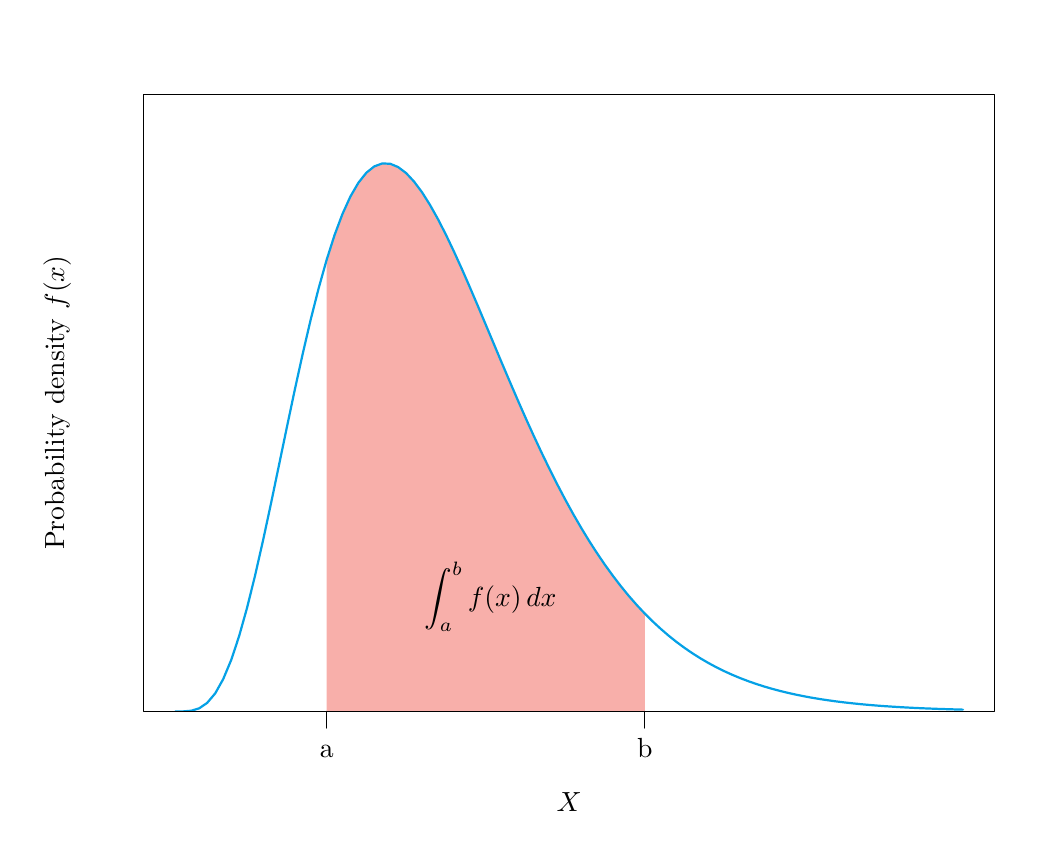
\begin{tikzpicture}[x=1pt,y=1pt]
\definecolor{fillColor}{RGB}{255,255,255}
\path[use as bounding box,fill=fillColor,fill opacity=0.00] (0,0) rectangle (361.35,289.08);
\begin{scope}
\path[clip] (  0.00,  0.00) rectangle (361.35,289.08);
\definecolor{drawColor}{RGB}{0,0,0}

\node[text=drawColor,anchor=base,inner sep=0pt, outer sep=0pt, scale=  1.00] at (195.67,  6.00) {$X$};

\node[text=drawColor,rotate= 90.00,anchor=base,inner sep=0pt, outer sep=0pt, scale=  1.00] at ( 13.20,153.54) {Probability density $f(x)$};
\end{scope}
\begin{scope}
\path[clip] (  0.00,  0.00) rectangle (361.35,289.08);
\definecolor{drawColor}{RGB}{0,0,0}

\path[draw=drawColor,line width= 0.4pt,line join=round,line cap=round] (108.00, 42.00) -- (222.98, 42.00);

\path[draw=drawColor,line width= 0.4pt,line join=round,line cap=round] (108.00, 42.00) -- (108.00, 36.00);

\path[draw=drawColor,line width= 0.4pt,line join=round,line cap=round] (222.98, 42.00) -- (222.98, 36.00);

\node[text=drawColor,anchor=base,inner sep=0pt, outer sep=0pt, scale=  1.00] at (108.00, 25.20) {a};

\node[text=drawColor,anchor=base,inner sep=0pt, outer sep=0pt, scale=  1.00] at (222.98, 25.20) {b};
\end{scope}
\begin{scope}
\path[clip] ( 42.00, 42.00) rectangle (349.35,265.08);
\definecolor{fillColor}{RGB}{238,50,36}

\path[fill=fillColor,fill opacity=0.39] (108.00, 42.00) --
	(108.00,205.09) --
	(110.87,214.08) --
	(113.75,221.76) --
	(116.62,228.08) --
	(119.50,233.03) --
	(122.37,236.65) --
	(125.25,238.95) --
	(128.12,240.01) --
	(131.00,239.90) --
	(133.87,238.71) --
	(136.75,236.53) --
	(139.62,233.46) --
	(142.50,229.60) --
	(145.37,225.05) --
	(148.24,219.92) --
	(151.12,214.30) --
	(153.99,208.28) --
	(156.87,201.95) --
	(159.74,195.38) --
	(162.62,188.66) --
	(165.49,181.84) --
	(168.37,174.99) --
	(171.24,168.15) --
	(174.12,161.39) --
	(176.99,154.73) --
	(179.86,148.21) --
	(182.74,141.86) --
	(185.61,135.71) --
	(188.49,129.77) --
	(191.36,124.06) --
	(194.24,118.58) --
	(197.11,113.35) --
	(199.99,108.38) --
	(202.86,103.65) --
	(205.74, 99.18) --
	(208.61, 94.96) --
	(211.49, 90.98) --
	(214.36, 87.24) --
	(217.23, 83.73) --
	(220.11, 80.44) --
	(222.98, 77.38) --
	(222.98, 42.00) --
	cycle;
\definecolor{drawColor}{RGB}{5,161,230}

\path[draw=drawColor,line width= 0.8pt,line join=round,line cap=round] ( 53.38, 42.00) --
	( 56.26, 42.02) --
	( 59.13, 42.26) --
	( 62.01, 43.14) --
	( 64.88, 45.11) --
	( 67.76, 48.52) --
	( 70.63, 53.63) --
	( 73.51, 60.51) --
	( 76.38, 69.14) --
	( 79.25, 79.36) --
	( 82.13, 90.94) --
	( 85.00,103.57) --
	( 87.88,116.95) --
	( 90.75,130.71) --
	( 93.63,144.55) --
	( 96.50,158.14) --
	( 99.38,171.21) --
	(102.25,183.52) --
	(105.13,194.86) --
	(108.00,205.09) --
	(110.87,214.08) --
	(113.75,221.76) --
	(116.62,228.08) --
	(119.50,233.03) --
	(122.37,236.65) --
	(125.25,238.95) --
	(128.12,240.01) --
	(131.00,239.90) --
	(133.87,238.71) --
	(136.75,236.53) --
	(139.62,233.46) --
	(142.50,229.60) --
	(145.37,225.05) --
	(148.24,219.92) --
	(151.12,214.30) --
	(153.99,208.28) --
	(156.87,201.95) --
	(159.74,195.38) --
	(162.62,188.66) --
	(165.49,181.84) --
	(168.37,174.99) --
	(171.24,168.15) --
	(174.12,161.39) --
	(176.99,154.73) --
	(179.86,148.21) --
	(182.74,141.86) --
	(185.61,135.71) --
	(188.49,129.77) --
	(191.36,124.06) --
	(194.24,118.58) --
	(197.11,113.35) --
	(199.99,108.38) --
	(202.86,103.65) --
	(205.74, 99.18) --
	(208.61, 94.96) --
	(211.49, 90.98) --
	(214.36, 87.24) --
	(217.23, 83.73) --
	(220.11, 80.44) --
	(222.98, 77.38) --
	(225.86, 74.52) --
	(228.73, 71.86) --
	(231.61, 69.38) --
	(234.48, 67.09) --
	(237.36, 64.96) --
	(240.23, 63.00) --
	(243.11, 61.18) --
	(245.98, 59.51) --
	(248.85, 57.96) --
	(251.73, 56.54) --
	(254.60, 55.24) --
	(257.48, 54.04) --
	(260.35, 52.95) --
	(263.23, 51.94) --
	(266.10, 51.02) --
	(268.98, 50.18) --
	(271.85, 49.41) --
	(274.73, 48.71) --
	(277.60, 48.07) --
	(280.48, 47.49) --
	(283.35, 46.96) --
	(286.22, 46.48) --
	(289.10, 46.05) --
	(291.97, 45.65) --
	(294.85, 45.29) --
	(297.72, 44.97) --
	(300.60, 44.67) --
	(303.47, 44.40) --
	(306.35, 44.16) --
	(309.22, 43.94) --
	(312.10, 43.75) --
	(314.97, 43.57) --
	(317.84, 43.41) --
	(320.72, 43.26) --
	(323.59, 43.13) --
	(326.47, 43.02) --
	(329.34, 42.91) --
	(332.22, 42.82) --
	(335.09, 42.73) --
	(337.97, 42.65);
\definecolor{drawColor}{RGB}{0,0,0}

\node[text=drawColor,anchor=base,inner sep=0pt, outer sep=0pt, scale=  1.00] at (167.22, 80.06) {$\displaystyle \int_a^b f(x)\,dx$};
\end{scope}
\begin{scope}
\path[clip] (  0.00,  0.00) rectangle (361.35,289.08);
\definecolor{drawColor}{RGB}{0,0,0}

\path[draw=drawColor,line width= 0.4pt,line join=round,line cap=round] ( 42.00, 42.00) --
	(349.35, 42.00) --
	(349.35,265.08) --
	( 42.00,265.08) --
	( 42.00, 42.00);
\end{scope}
\end{tikzpicture}
}}
\mode<presentation>{\resizebox{0.7\textwidth}{!}{% Created by tikzDevice version 0.9 on 2016-04-28 16:54:50
% !TEX encoding = UTF-8 Unicode
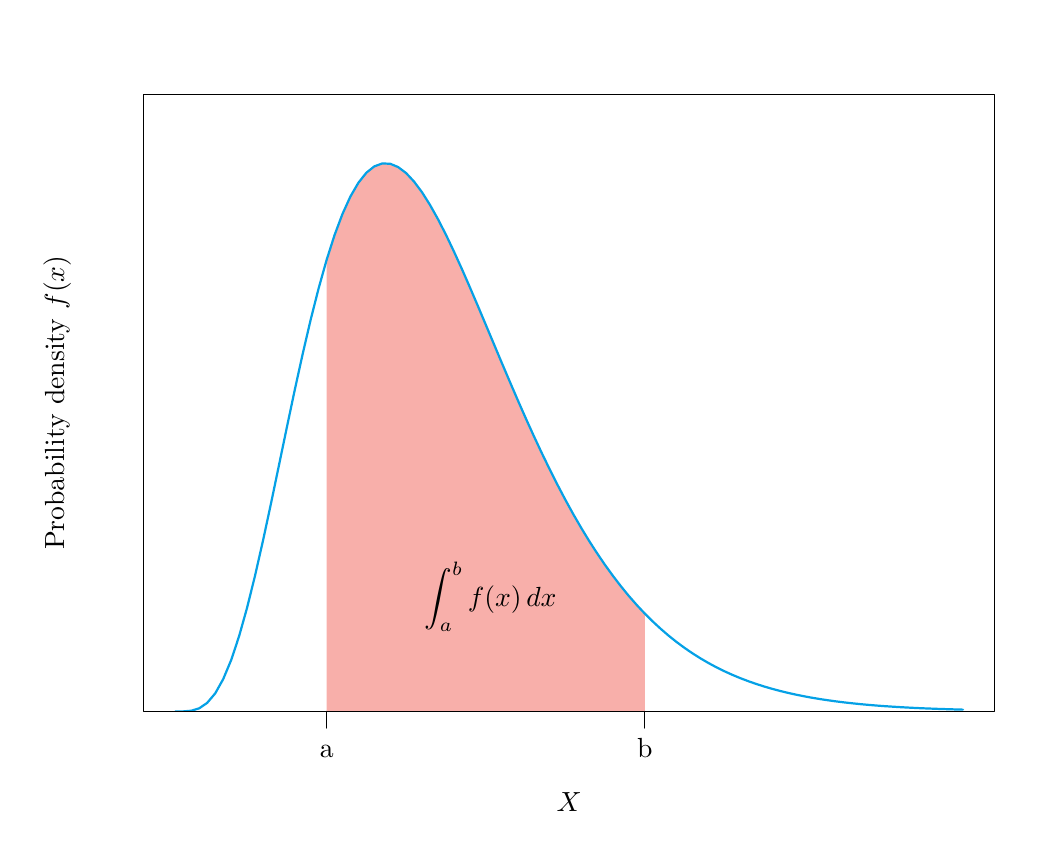
\begin{tikzpicture}[x=1pt,y=1pt]
\definecolor{fillColor}{RGB}{255,255,255}
\path[use as bounding box,fill=fillColor,fill opacity=0.00] (0,0) rectangle (361.35,289.08);
\begin{scope}
\path[clip] (  0.00,  0.00) rectangle (361.35,289.08);
\definecolor{drawColor}{RGB}{0,0,0}

\node[text=drawColor,anchor=base,inner sep=0pt, outer sep=0pt, scale=  1.00] at (195.67,  6.00) {$X$};

\node[text=drawColor,rotate= 90.00,anchor=base,inner sep=0pt, outer sep=0pt, scale=  1.00] at ( 13.20,153.54) {Probability density $f(x)$};
\end{scope}
\begin{scope}
\path[clip] (  0.00,  0.00) rectangle (361.35,289.08);
\definecolor{drawColor}{RGB}{0,0,0}

\path[draw=drawColor,line width= 0.4pt,line join=round,line cap=round] (108.00, 42.00) -- (222.98, 42.00);

\path[draw=drawColor,line width= 0.4pt,line join=round,line cap=round] (108.00, 42.00) -- (108.00, 36.00);

\path[draw=drawColor,line width= 0.4pt,line join=round,line cap=round] (222.98, 42.00) -- (222.98, 36.00);

\node[text=drawColor,anchor=base,inner sep=0pt, outer sep=0pt, scale=  1.00] at (108.00, 25.20) {a};

\node[text=drawColor,anchor=base,inner sep=0pt, outer sep=0pt, scale=  1.00] at (222.98, 25.20) {b};
\end{scope}
\begin{scope}
\path[clip] ( 42.00, 42.00) rectangle (349.35,265.08);
\definecolor{fillColor}{RGB}{238,50,36}

\path[fill=fillColor,fill opacity=0.39] (108.00, 42.00) --
	(108.00,205.09) --
	(110.87,214.08) --
	(113.75,221.76) --
	(116.62,228.08) --
	(119.50,233.03) --
	(122.37,236.65) --
	(125.25,238.95) --
	(128.12,240.01) --
	(131.00,239.90) --
	(133.87,238.71) --
	(136.75,236.53) --
	(139.62,233.46) --
	(142.50,229.60) --
	(145.37,225.05) --
	(148.24,219.92) --
	(151.12,214.30) --
	(153.99,208.28) --
	(156.87,201.95) --
	(159.74,195.38) --
	(162.62,188.66) --
	(165.49,181.84) --
	(168.37,174.99) --
	(171.24,168.15) --
	(174.12,161.39) --
	(176.99,154.73) --
	(179.86,148.21) --
	(182.74,141.86) --
	(185.61,135.71) --
	(188.49,129.77) --
	(191.36,124.06) --
	(194.24,118.58) --
	(197.11,113.35) --
	(199.99,108.38) --
	(202.86,103.65) --
	(205.74, 99.18) --
	(208.61, 94.96) --
	(211.49, 90.98) --
	(214.36, 87.24) --
	(217.23, 83.73) --
	(220.11, 80.44) --
	(222.98, 77.38) --
	(222.98, 42.00) --
	cycle;
\definecolor{drawColor}{RGB}{5,161,230}

\path[draw=drawColor,line width= 0.8pt,line join=round,line cap=round] ( 53.38, 42.00) --
	( 56.26, 42.02) --
	( 59.13, 42.26) --
	( 62.01, 43.14) --
	( 64.88, 45.11) --
	( 67.76, 48.52) --
	( 70.63, 53.63) --
	( 73.51, 60.51) --
	( 76.38, 69.14) --
	( 79.25, 79.36) --
	( 82.13, 90.94) --
	( 85.00,103.57) --
	( 87.88,116.95) --
	( 90.75,130.71) --
	( 93.63,144.55) --
	( 96.50,158.14) --
	( 99.38,171.21) --
	(102.25,183.52) --
	(105.13,194.86) --
	(108.00,205.09) --
	(110.87,214.08) --
	(113.75,221.76) --
	(116.62,228.08) --
	(119.50,233.03) --
	(122.37,236.65) --
	(125.25,238.95) --
	(128.12,240.01) --
	(131.00,239.90) --
	(133.87,238.71) --
	(136.75,236.53) --
	(139.62,233.46) --
	(142.50,229.60) --
	(145.37,225.05) --
	(148.24,219.92) --
	(151.12,214.30) --
	(153.99,208.28) --
	(156.87,201.95) --
	(159.74,195.38) --
	(162.62,188.66) --
	(165.49,181.84) --
	(168.37,174.99) --
	(171.24,168.15) --
	(174.12,161.39) --
	(176.99,154.73) --
	(179.86,148.21) --
	(182.74,141.86) --
	(185.61,135.71) --
	(188.49,129.77) --
	(191.36,124.06) --
	(194.24,118.58) --
	(197.11,113.35) --
	(199.99,108.38) --
	(202.86,103.65) --
	(205.74, 99.18) --
	(208.61, 94.96) --
	(211.49, 90.98) --
	(214.36, 87.24) --
	(217.23, 83.73) --
	(220.11, 80.44) --
	(222.98, 77.38) --
	(225.86, 74.52) --
	(228.73, 71.86) --
	(231.61, 69.38) --
	(234.48, 67.09) --
	(237.36, 64.96) --
	(240.23, 63.00) --
	(243.11, 61.18) --
	(245.98, 59.51) --
	(248.85, 57.96) --
	(251.73, 56.54) --
	(254.60, 55.24) --
	(257.48, 54.04) --
	(260.35, 52.95) --
	(263.23, 51.94) --
	(266.10, 51.02) --
	(268.98, 50.18) --
	(271.85, 49.41) --
	(274.73, 48.71) --
	(277.60, 48.07) --
	(280.48, 47.49) --
	(283.35, 46.96) --
	(286.22, 46.48) --
	(289.10, 46.05) --
	(291.97, 45.65) --
	(294.85, 45.29) --
	(297.72, 44.97) --
	(300.60, 44.67) --
	(303.47, 44.40) --
	(306.35, 44.16) --
	(309.22, 43.94) --
	(312.10, 43.75) --
	(314.97, 43.57) --
	(317.84, 43.41) --
	(320.72, 43.26) --
	(323.59, 43.13) --
	(326.47, 43.02) --
	(329.34, 42.91) --
	(332.22, 42.82) --
	(335.09, 42.73) --
	(337.97, 42.65);
\definecolor{drawColor}{RGB}{0,0,0}

\node[text=drawColor,anchor=base,inner sep=0pt, outer sep=0pt, scale=  1.00] at (167.22, 80.06) {$\displaystyle \int_a^b f(x)\,dx$};
\end{scope}
\begin{scope}
\path[clip] (  0.00,  0.00) rectangle (361.35,289.08);
\definecolor{drawColor}{RGB}{0,0,0}

\path[draw=drawColor,line width= 0.4pt,line join=round,line cap=round] ( 42.00, 42.00) --
	(349.35, 42.00) --
	(349.35,265.08) --
	( 42.00,265.08) --
	( 42.00, 42.00);
\end{scope}
\end{tikzpicture}
}}
$\displaystyle P(a\leq X\leq b) = \int_a^b f(x)\, dx = F(b)-F(a)$
\end{center}
\end{frame}



%---------------------------------------------------------------------slide----
\begin{frame}
\frametitle{Probabilities as areas}
\framesubtitle{Example}
Given the following function
\[
f(x) =
\begin{cases}
0 & \mbox{si $x<0$}\\
e^{-x} & \mbox{si $x\geq 0$},
\end{cases}
\]
let's check that is a density function. 

As this function is clearly non-negative, we have to check that total area bounded by the curve and the x-axis is 1.

\begin{align*}
\int_{-\infty}^\infty f(x)\;dx &= \int_{-\infty}^0 f(x)\;dx +\int_0^\infty f(x)\;dx = \int_{-\infty}^0 0\;dx +\int_0^\infty e^{-x}\;dx =\\
&= \left[-e^{-x}\right]_0^{\infty} = -e^{-\infty}+e^0 = 1.
\end{align*}

Now, let's calculate the probability of $X$ having a value between 0 and 2. 

\begin{align*}
P(0\leq X\leq 2) &= \int_0^2 f(x)\;dx = \int_0^2 e^{-x}\;dx = \left[-e^{-x}\right]_0^2 = -e^{-2}+e^0 = 0.8646.
\end{align*}
\end{frame}


%---------------------------------------------------------------------slide----
\begin{frame}
\frametitle{Population statistics}
The calculation of the population statistics is similar to the case of discrete variables, but using the density function instead of the probability function, and extending the discrete sum to the integral.

The most important are:
\begin{itemize}
\item \structure{Mean}:
\[
\mu = E(X) = \int_{-\infty}^\infty x f(x)\; dx
\]
\item \structure{Variance}:
\[
\sigma^2 = Var(X) = \int_{-\infty}^\infty x^2f(x)\; dx -\mu^2
\]
\item \structure{Standard deviation}:
\[
\sigma = +\sqrt{\sigma^2}
\]
\end{itemize}
\end{frame}


%---------------------------------------------------------------------slide----
\begin{frame}
\frametitle{Population statistics}
\framesubtitle{Example}
Let $X$ be a variable with the following Densidad de probabilidad function
\[
f(x) =
\begin{cases}
0 & \mbox{si $x<0$}\\
e^{-x} & \mbox{si $x\geq 0$}
\end{cases}
\]

The mean is 

\begin{align*}
\mu &= \int_{-\infty}^\infty xf(x)\;dx = \int_{-\infty}^0 xf(x)\;dx +\int_0^\infty xf(x)\;dx = \int_{-\infty}^0 0\;dx +\int_0^\infty xe^{-x}\;dx =\\
&= \left[-e^{-x}(1+x)\right]_0^{\infty} = 1.
\end{align*}

and the variance is

\begin{align*}
\sigma^2 &= \int_{-\infty}^\infty x^2f(x)\;dx -\mu^2 = \int_{-\infty}^0 x^2f(x)\;dx +\int_0^\infty x^2f(x)\;dx -\mu^2 = \\
&= \int_{-\infty}^0 0\;dx +\int_0^\infty x^2e^{-x}\;dx -\mu^2= \left[-e^{-x}(x^2+2x+2)\right]_0^{\infty} - 1^2= 2e^0-1 = 1.
\end{align*}

\end{frame}



%---------------------------------------------------------------------slide----
\begin{frame}
\frametitle{Continuous probability distribution models}
According to the type of experiment where the random variable is measured, there are different probability distributions models. 
The most common are:
\begin{itemize}
\item Continuous uniform.
\item Normal.
\item Student's T.
\item Chi-square.
\item Fisher-Snedecor's F.
\end{itemize}
\end{frame}


\subsection{Continuous uniform distribution}

%---------------------------------------------------------------------slide----
\begin{frame}
\frametitle{Continuous uniform probability distribution model $U(a,b)$}
When all the values of a random variable $X$ have equal probability, the probability distribution of $X$ is uniform.

\begin{definition}[Continuous uniform distribution $U(a,b)$]
A continuous random variable $X$ follows a probability distribution model \emph{uniform} of parameters $a$ and
$b$, noted $X\sim U(a,b)$, if its range is $\mbox{Ran}(X) = [a,b]$ and its density function is
\[
f(x)= \frac{1}{b-a}\quad \forall x\in [a,b]
\]
\end{definition}

Observe that $a$ and $b$ are the minimum and the maximum of the range respectively, and that the density function is constant. 

The mean and the variance are
\[
\mu = \frac{a+b}{2}\qquad \sigma^2=\frac{(b-a)^2}{12}.
\]
\end{frame}


%---------------------------------------------------------------------slide----
\begin{frame}
\frametitle{Continuous uniform Densidad de probabilidad function}
\framesubtitle{Example}

The generation of a random number between 0 and 1 is follows a continuous uniform distribution $U(0,1)$.
\begin{center}
\tikzsetnextfilename{continuous_random_variables/uniform_density_function}
\mode<article>{\resizebox{0.6\textwidth}{!}{% Created by tikzDevice version 0.9 on 2016-04-28 17:31:47
% !TEX encoding = UTF-8 Unicode
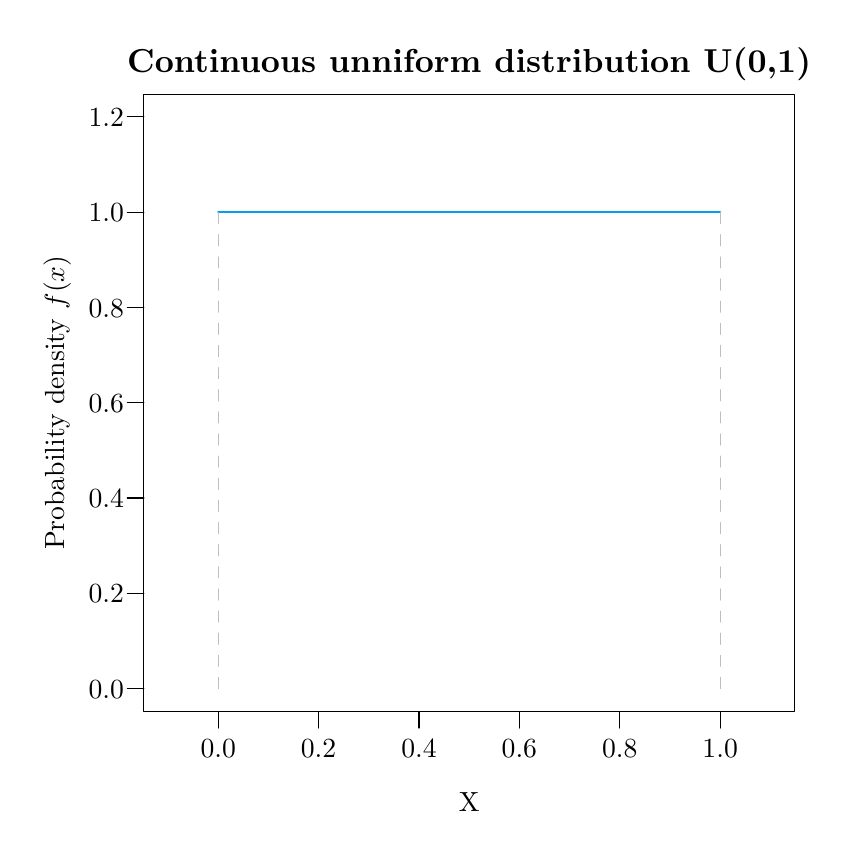
\begin{tikzpicture}[x=1pt,y=1pt]
\definecolor{fillColor}{RGB}{255,255,255}
\path[use as bounding box,fill=fillColor,fill opacity=0.00] (0,0) rectangle (289.08,289.08);
\begin{scope}
\path[clip] ( 42.00, 42.00) rectangle (277.08,265.08);
\definecolor{drawColor}{RGB}{5,161,230}

\path[draw=drawColor,line width= 0.8pt,line join=round,line cap=round] ( 68.85,222.39) --
	( 89.00,222.39) --
	(109.15,222.39) --
	(129.31,222.39) --
	(149.46,222.39) --
	(169.62,222.39) --
	(189.77,222.39) --
	(209.93,222.39) --
	(230.08,222.39) --
	(250.23,222.39);
\end{scope}
\begin{scope}
\path[clip] (  0.00,  0.00) rectangle (289.08,289.08);
\definecolor{drawColor}{RGB}{0,0,0}

\path[draw=drawColor,line width= 0.4pt,line join=round,line cap=round] ( 68.85, 42.00) -- (250.23, 42.00);

\path[draw=drawColor,line width= 0.4pt,line join=round,line cap=round] ( 68.85, 42.00) -- ( 68.85, 36.00);

\path[draw=drawColor,line width= 0.4pt,line join=round,line cap=round] (105.12, 42.00) -- (105.12, 36.00);

\path[draw=drawColor,line width= 0.4pt,line join=round,line cap=round] (141.40, 42.00) -- (141.40, 36.00);

\path[draw=drawColor,line width= 0.4pt,line join=round,line cap=round] (177.68, 42.00) -- (177.68, 36.00);

\path[draw=drawColor,line width= 0.4pt,line join=round,line cap=round] (213.96, 42.00) -- (213.96, 36.00);

\path[draw=drawColor,line width= 0.4pt,line join=round,line cap=round] (250.23, 42.00) -- (250.23, 36.00);

\node[text=drawColor,anchor=base,inner sep=0pt, outer sep=0pt, scale=  1.00] at ( 68.85, 25.20) {0.0};

\node[text=drawColor,anchor=base,inner sep=0pt, outer sep=0pt, scale=  1.00] at (105.12, 25.20) {0.2};

\node[text=drawColor,anchor=base,inner sep=0pt, outer sep=0pt, scale=  1.00] at (141.40, 25.20) {0.4};

\node[text=drawColor,anchor=base,inner sep=0pt, outer sep=0pt, scale=  1.00] at (177.68, 25.20) {0.6};

\node[text=drawColor,anchor=base,inner sep=0pt, outer sep=0pt, scale=  1.00] at (213.96, 25.20) {0.8};

\node[text=drawColor,anchor=base,inner sep=0pt, outer sep=0pt, scale=  1.00] at (250.23, 25.20) {1.0};

\path[draw=drawColor,line width= 0.4pt,line join=round,line cap=round] ( 42.00, 50.26) -- ( 42.00,256.82);

\path[draw=drawColor,line width= 0.4pt,line join=round,line cap=round] ( 42.00, 50.26) -- ( 36.00, 50.26);

\path[draw=drawColor,line width= 0.4pt,line join=round,line cap=round] ( 42.00, 84.69) -- ( 36.00, 84.69);

\path[draw=drawColor,line width= 0.4pt,line join=round,line cap=round] ( 42.00,119.11) -- ( 36.00,119.11);

\path[draw=drawColor,line width= 0.4pt,line join=round,line cap=round] ( 42.00,153.54) -- ( 36.00,153.54);

\path[draw=drawColor,line width= 0.4pt,line join=round,line cap=round] ( 42.00,187.97) -- ( 36.00,187.97);

\path[draw=drawColor,line width= 0.4pt,line join=round,line cap=round] ( 42.00,222.39) -- ( 36.00,222.39);

\path[draw=drawColor,line width= 0.4pt,line join=round,line cap=round] ( 42.00,256.82) -- ( 36.00,256.82);

\node[text=drawColor,anchor=base east,inner sep=0pt, outer sep=0pt, scale=  1.00] at ( 34.80, 46.82) {0.0};

\node[text=drawColor,anchor=base east,inner sep=0pt, outer sep=0pt, scale=  1.00] at ( 34.80, 81.24) {0.2};

\node[text=drawColor,anchor=base east,inner sep=0pt, outer sep=0pt, scale=  1.00] at ( 34.80,115.67) {0.4};

\node[text=drawColor,anchor=base east,inner sep=0pt, outer sep=0pt, scale=  1.00] at ( 34.80,150.10) {0.6};

\node[text=drawColor,anchor=base east,inner sep=0pt, outer sep=0pt, scale=  1.00] at ( 34.80,184.52) {0.8};

\node[text=drawColor,anchor=base east,inner sep=0pt, outer sep=0pt, scale=  1.00] at ( 34.80,218.95) {1.0};

\node[text=drawColor,anchor=base east,inner sep=0pt, outer sep=0pt, scale=  1.00] at ( 34.80,253.37) {1.2};

\path[draw=drawColor,line width= 0.4pt,line join=round,line cap=round] ( 42.00, 42.00) --
	(277.08, 42.00) --
	(277.08,265.08) --
	( 42.00,265.08) --
	( 42.00, 42.00);
\end{scope}
\begin{scope}
\path[clip] (  0.00,  0.00) rectangle (289.08,289.08);
\definecolor{drawColor}{RGB}{0,0,0}

\node[text=drawColor,anchor=base,inner sep=0pt, outer sep=0pt, scale=  1.20] at (159.54,272.89) {\bfseries Continuous unniform distribution U(0,1)};

\node[text=drawColor,anchor=base,inner sep=0pt, outer sep=0pt, scale=  1.00] at (159.54,  6.00) {X};

\node[text=drawColor,rotate= 90.00,anchor=base,inner sep=0pt, outer sep=0pt, scale=  1.00] at ( 13.20,153.54) {Probability density $f(x)$};
\end{scope}
\begin{scope}
\path[clip] ( 42.00, 42.00) rectangle (277.08,265.08);
\definecolor{drawColor}{RGB}{190,190,190}

\path[draw=drawColor,line width= 0.4pt,dash pattern=on 4pt off 4pt ,line join=round,line cap=round] ( 68.85, 50.26) -- ( 68.85,222.39);

\path[draw=drawColor,line width= 0.4pt,dash pattern=on 4pt off 4pt ,line join=round,line cap=round] (250.23, 50.26) -- (250.23,222.39);
\end{scope}
\end{tikzpicture}
}}
\mode<presentation>{\resizebox{0.6\textwidth}{!}{% Created by tikzDevice version 0.9 on 2016-04-28 17:31:47
% !TEX encoding = UTF-8 Unicode
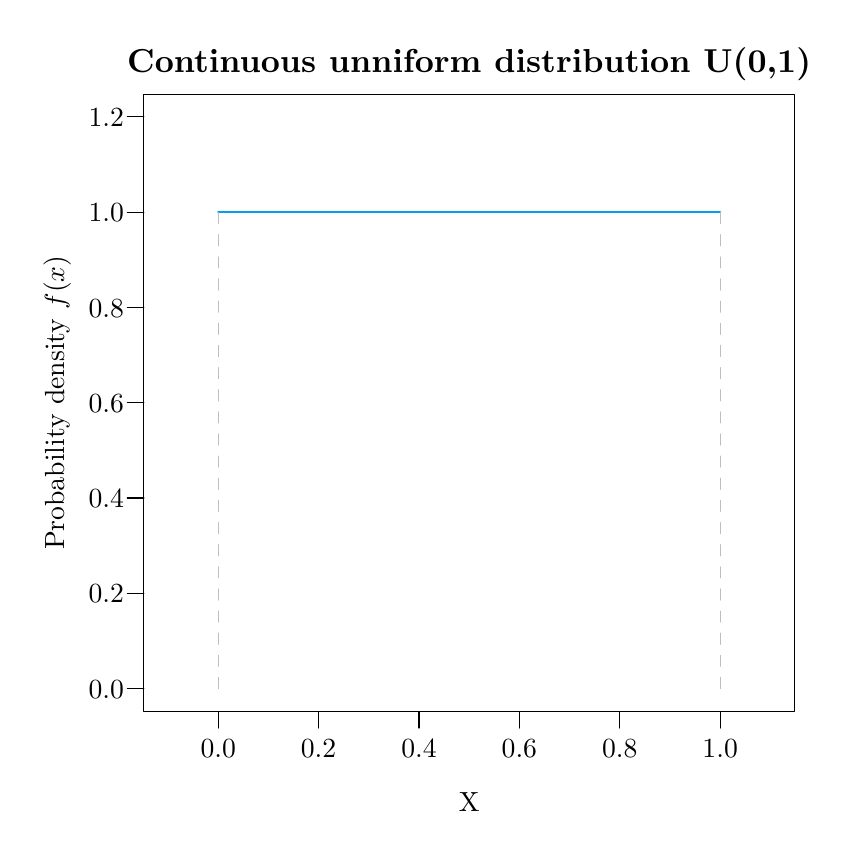
\begin{tikzpicture}[x=1pt,y=1pt]
\definecolor{fillColor}{RGB}{255,255,255}
\path[use as bounding box,fill=fillColor,fill opacity=0.00] (0,0) rectangle (289.08,289.08);
\begin{scope}
\path[clip] ( 42.00, 42.00) rectangle (277.08,265.08);
\definecolor{drawColor}{RGB}{5,161,230}

\path[draw=drawColor,line width= 0.8pt,line join=round,line cap=round] ( 68.85,222.39) --
	( 89.00,222.39) --
	(109.15,222.39) --
	(129.31,222.39) --
	(149.46,222.39) --
	(169.62,222.39) --
	(189.77,222.39) --
	(209.93,222.39) --
	(230.08,222.39) --
	(250.23,222.39);
\end{scope}
\begin{scope}
\path[clip] (  0.00,  0.00) rectangle (289.08,289.08);
\definecolor{drawColor}{RGB}{0,0,0}

\path[draw=drawColor,line width= 0.4pt,line join=round,line cap=round] ( 68.85, 42.00) -- (250.23, 42.00);

\path[draw=drawColor,line width= 0.4pt,line join=round,line cap=round] ( 68.85, 42.00) -- ( 68.85, 36.00);

\path[draw=drawColor,line width= 0.4pt,line join=round,line cap=round] (105.12, 42.00) -- (105.12, 36.00);

\path[draw=drawColor,line width= 0.4pt,line join=round,line cap=round] (141.40, 42.00) -- (141.40, 36.00);

\path[draw=drawColor,line width= 0.4pt,line join=round,line cap=round] (177.68, 42.00) -- (177.68, 36.00);

\path[draw=drawColor,line width= 0.4pt,line join=round,line cap=round] (213.96, 42.00) -- (213.96, 36.00);

\path[draw=drawColor,line width= 0.4pt,line join=round,line cap=round] (250.23, 42.00) -- (250.23, 36.00);

\node[text=drawColor,anchor=base,inner sep=0pt, outer sep=0pt, scale=  1.00] at ( 68.85, 25.20) {0.0};

\node[text=drawColor,anchor=base,inner sep=0pt, outer sep=0pt, scale=  1.00] at (105.12, 25.20) {0.2};

\node[text=drawColor,anchor=base,inner sep=0pt, outer sep=0pt, scale=  1.00] at (141.40, 25.20) {0.4};

\node[text=drawColor,anchor=base,inner sep=0pt, outer sep=0pt, scale=  1.00] at (177.68, 25.20) {0.6};

\node[text=drawColor,anchor=base,inner sep=0pt, outer sep=0pt, scale=  1.00] at (213.96, 25.20) {0.8};

\node[text=drawColor,anchor=base,inner sep=0pt, outer sep=0pt, scale=  1.00] at (250.23, 25.20) {1.0};

\path[draw=drawColor,line width= 0.4pt,line join=round,line cap=round] ( 42.00, 50.26) -- ( 42.00,256.82);

\path[draw=drawColor,line width= 0.4pt,line join=round,line cap=round] ( 42.00, 50.26) -- ( 36.00, 50.26);

\path[draw=drawColor,line width= 0.4pt,line join=round,line cap=round] ( 42.00, 84.69) -- ( 36.00, 84.69);

\path[draw=drawColor,line width= 0.4pt,line join=round,line cap=round] ( 42.00,119.11) -- ( 36.00,119.11);

\path[draw=drawColor,line width= 0.4pt,line join=round,line cap=round] ( 42.00,153.54) -- ( 36.00,153.54);

\path[draw=drawColor,line width= 0.4pt,line join=round,line cap=round] ( 42.00,187.97) -- ( 36.00,187.97);

\path[draw=drawColor,line width= 0.4pt,line join=round,line cap=round] ( 42.00,222.39) -- ( 36.00,222.39);

\path[draw=drawColor,line width= 0.4pt,line join=round,line cap=round] ( 42.00,256.82) -- ( 36.00,256.82);

\node[text=drawColor,anchor=base east,inner sep=0pt, outer sep=0pt, scale=  1.00] at ( 34.80, 46.82) {0.0};

\node[text=drawColor,anchor=base east,inner sep=0pt, outer sep=0pt, scale=  1.00] at ( 34.80, 81.24) {0.2};

\node[text=drawColor,anchor=base east,inner sep=0pt, outer sep=0pt, scale=  1.00] at ( 34.80,115.67) {0.4};

\node[text=drawColor,anchor=base east,inner sep=0pt, outer sep=0pt, scale=  1.00] at ( 34.80,150.10) {0.6};

\node[text=drawColor,anchor=base east,inner sep=0pt, outer sep=0pt, scale=  1.00] at ( 34.80,184.52) {0.8};

\node[text=drawColor,anchor=base east,inner sep=0pt, outer sep=0pt, scale=  1.00] at ( 34.80,218.95) {1.0};

\node[text=drawColor,anchor=base east,inner sep=0pt, outer sep=0pt, scale=  1.00] at ( 34.80,253.37) {1.2};

\path[draw=drawColor,line width= 0.4pt,line join=round,line cap=round] ( 42.00, 42.00) --
	(277.08, 42.00) --
	(277.08,265.08) --
	( 42.00,265.08) --
	( 42.00, 42.00);
\end{scope}
\begin{scope}
\path[clip] (  0.00,  0.00) rectangle (289.08,289.08);
\definecolor{drawColor}{RGB}{0,0,0}

\node[text=drawColor,anchor=base,inner sep=0pt, outer sep=0pt, scale=  1.20] at (159.54,272.89) {\bfseries Continuous unniform distribution U(0,1)};

\node[text=drawColor,anchor=base,inner sep=0pt, outer sep=0pt, scale=  1.00] at (159.54,  6.00) {X};

\node[text=drawColor,rotate= 90.00,anchor=base,inner sep=0pt, outer sep=0pt, scale=  1.00] at ( 13.20,153.54) {Probability density $f(x)$};
\end{scope}
\begin{scope}
\path[clip] ( 42.00, 42.00) rectangle (277.08,265.08);
\definecolor{drawColor}{RGB}{190,190,190}

\path[draw=drawColor,line width= 0.4pt,dash pattern=on 4pt off 4pt ,line join=round,line cap=round] ( 68.85, 50.26) -- ( 68.85,222.39);

\path[draw=drawColor,line width= 0.4pt,dash pattern=on 4pt off 4pt ,line join=round,line cap=round] (250.23, 50.26) -- (250.23,222.39);
\end{scope}
\end{tikzpicture}
}}
\end{center}
\end{frame}


%---------------------------------------------------------------------slide----
\begin{frame}
\frametitle{Continuous uniform distribution function}
\framesubtitle{Example}
As the density function is constant, the distribution function has a linear growth. 
\begin{center}
\tikzsetnextfilename{continuous_random_variables/uniform_distribution_function}
\mode<article>{\resizebox{0.6\textwidth}{!}{% Created by tikzDevice version 0.9 on 2016-04-28 17:47:04
% !TEX encoding = UTF-8 Unicode
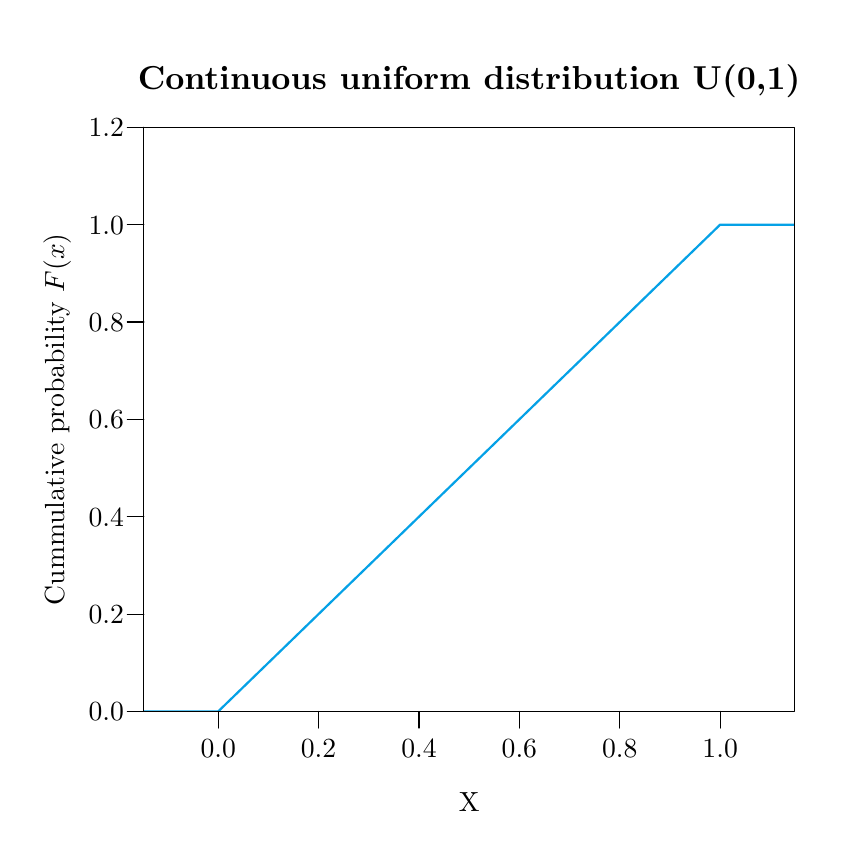
\begin{tikzpicture}[x=1pt,y=1pt]
\definecolor{fillColor}{RGB}{255,255,255}
\path[use as bounding box,fill=fillColor,fill opacity=0.00] (0,0) rectangle (289.08,289.08);
\begin{scope}
\path[clip] ( 42.00, 42.00) rectangle (277.08,253.08);
\definecolor{drawColor}{RGB}{5,161,230}

\path[draw=drawColor,line width= 0.8pt,line join=round,line cap=round] ( 32.57, 42.00) --
	( 68.85, 42.00) --
	( 89.00, 61.54) --
	(109.15, 81.09) --
	(129.31,100.63) --
	(149.46,120.18) --
	(169.62,139.72) --
	(189.77,159.27) --
	(209.93,178.81) --
	(230.08,198.36) --
	(250.23,217.90) --
	(286.51,217.90);
\end{scope}
\begin{scope}
\path[clip] (  0.00,  0.00) rectangle (289.08,289.08);
\definecolor{drawColor}{RGB}{0,0,0}

\path[draw=drawColor,line width= 0.4pt,line join=round,line cap=round] ( 68.85, 42.00) -- (250.23, 42.00);

\path[draw=drawColor,line width= 0.4pt,line join=round,line cap=round] ( 68.85, 42.00) -- ( 68.85, 36.00);

\path[draw=drawColor,line width= 0.4pt,line join=round,line cap=round] (105.12, 42.00) -- (105.12, 36.00);

\path[draw=drawColor,line width= 0.4pt,line join=round,line cap=round] (141.40, 42.00) -- (141.40, 36.00);

\path[draw=drawColor,line width= 0.4pt,line join=round,line cap=round] (177.68, 42.00) -- (177.68, 36.00);

\path[draw=drawColor,line width= 0.4pt,line join=round,line cap=round] (213.96, 42.00) -- (213.96, 36.00);

\path[draw=drawColor,line width= 0.4pt,line join=round,line cap=round] (250.23, 42.00) -- (250.23, 36.00);

\node[text=drawColor,anchor=base,inner sep=0pt, outer sep=0pt, scale=  1.00] at ( 68.85, 25.20) {0.0};

\node[text=drawColor,anchor=base,inner sep=0pt, outer sep=0pt, scale=  1.00] at (105.12, 25.20) {0.2};

\node[text=drawColor,anchor=base,inner sep=0pt, outer sep=0pt, scale=  1.00] at (141.40, 25.20) {0.4};

\node[text=drawColor,anchor=base,inner sep=0pt, outer sep=0pt, scale=  1.00] at (177.68, 25.20) {0.6};

\node[text=drawColor,anchor=base,inner sep=0pt, outer sep=0pt, scale=  1.00] at (213.96, 25.20) {0.8};

\node[text=drawColor,anchor=base,inner sep=0pt, outer sep=0pt, scale=  1.00] at (250.23, 25.20) {1.0};

\path[draw=drawColor,line width= 0.4pt,line join=round,line cap=round] ( 42.00, 42.00) -- ( 42.00,253.08);

\path[draw=drawColor,line width= 0.4pt,line join=round,line cap=round] ( 42.00, 42.00) -- ( 36.00, 42.00);

\path[draw=drawColor,line width= 0.4pt,line join=round,line cap=round] ( 42.00, 77.18) -- ( 36.00, 77.18);

\path[draw=drawColor,line width= 0.4pt,line join=round,line cap=round] ( 42.00,112.36) -- ( 36.00,112.36);

\path[draw=drawColor,line width= 0.4pt,line join=round,line cap=round] ( 42.00,147.54) -- ( 36.00,147.54);

\path[draw=drawColor,line width= 0.4pt,line join=round,line cap=round] ( 42.00,182.72) -- ( 36.00,182.72);

\path[draw=drawColor,line width= 0.4pt,line join=round,line cap=round] ( 42.00,217.90) -- ( 36.00,217.90);

\path[draw=drawColor,line width= 0.4pt,line join=round,line cap=round] ( 42.00,253.08) -- ( 36.00,253.08);

\node[text=drawColor,anchor=base east,inner sep=0pt, outer sep=0pt, scale=  1.00] at ( 34.80, 38.56) {0.0};

\node[text=drawColor,anchor=base east,inner sep=0pt, outer sep=0pt, scale=  1.00] at ( 34.80, 73.74) {0.2};

\node[text=drawColor,anchor=base east,inner sep=0pt, outer sep=0pt, scale=  1.00] at ( 34.80,108.92) {0.4};

\node[text=drawColor,anchor=base east,inner sep=0pt, outer sep=0pt, scale=  1.00] at ( 34.80,144.10) {0.6};

\node[text=drawColor,anchor=base east,inner sep=0pt, outer sep=0pt, scale=  1.00] at ( 34.80,179.28) {0.8};

\node[text=drawColor,anchor=base east,inner sep=0pt, outer sep=0pt, scale=  1.00] at ( 34.80,214.46) {1.0};

\node[text=drawColor,anchor=base east,inner sep=0pt, outer sep=0pt, scale=  1.00] at ( 34.80,249.64) {1.2};

\path[draw=drawColor,line width= 0.4pt,line join=round,line cap=round] ( 42.00, 42.00) --
	(277.08, 42.00) --
	(277.08,253.08) --
	( 42.00,253.08) --
	( 42.00, 42.00);
\end{scope}
\begin{scope}
\path[clip] (  0.00,  0.00) rectangle (289.08,289.08);
\definecolor{drawColor}{RGB}{0,0,0}

\node[text=drawColor,anchor=base,inner sep=0pt, outer sep=0pt, scale=  1.20] at (159.54,266.89) {\bfseries Continuous uniform distribution U(0,1)};

\node[text=drawColor,anchor=base,inner sep=0pt, outer sep=0pt, scale=  1.00] at (159.54,  6.00) {X};

\node[text=drawColor,rotate= 90.00,anchor=base,inner sep=0pt, outer sep=0pt, scale=  1.00] at ( 13.20,147.54) {Cummulative probability $F(x)$};
\end{scope}
\end{tikzpicture}
}}
\mode<presentation>{\resizebox{0.6\textwidth}{!}{% Created by tikzDevice version 0.9 on 2016-04-28 17:47:04
% !TEX encoding = UTF-8 Unicode
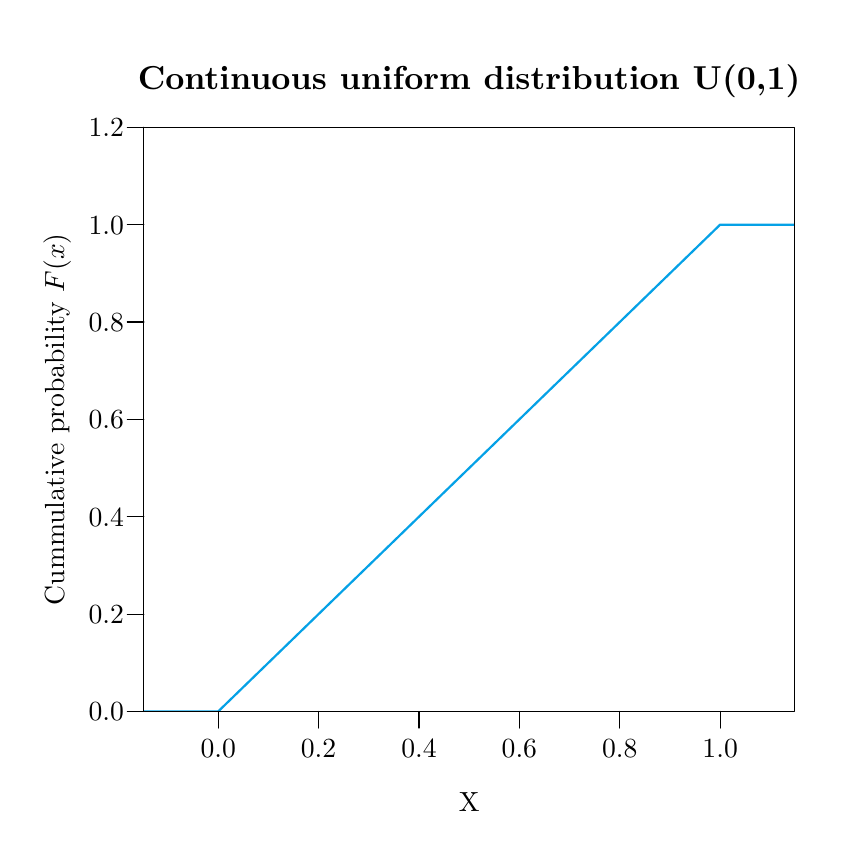
\begin{tikzpicture}[x=1pt,y=1pt]
\definecolor{fillColor}{RGB}{255,255,255}
\path[use as bounding box,fill=fillColor,fill opacity=0.00] (0,0) rectangle (289.08,289.08);
\begin{scope}
\path[clip] ( 42.00, 42.00) rectangle (277.08,253.08);
\definecolor{drawColor}{RGB}{5,161,230}

\path[draw=drawColor,line width= 0.8pt,line join=round,line cap=round] ( 32.57, 42.00) --
	( 68.85, 42.00) --
	( 89.00, 61.54) --
	(109.15, 81.09) --
	(129.31,100.63) --
	(149.46,120.18) --
	(169.62,139.72) --
	(189.77,159.27) --
	(209.93,178.81) --
	(230.08,198.36) --
	(250.23,217.90) --
	(286.51,217.90);
\end{scope}
\begin{scope}
\path[clip] (  0.00,  0.00) rectangle (289.08,289.08);
\definecolor{drawColor}{RGB}{0,0,0}

\path[draw=drawColor,line width= 0.4pt,line join=round,line cap=round] ( 68.85, 42.00) -- (250.23, 42.00);

\path[draw=drawColor,line width= 0.4pt,line join=round,line cap=round] ( 68.85, 42.00) -- ( 68.85, 36.00);

\path[draw=drawColor,line width= 0.4pt,line join=round,line cap=round] (105.12, 42.00) -- (105.12, 36.00);

\path[draw=drawColor,line width= 0.4pt,line join=round,line cap=round] (141.40, 42.00) -- (141.40, 36.00);

\path[draw=drawColor,line width= 0.4pt,line join=round,line cap=round] (177.68, 42.00) -- (177.68, 36.00);

\path[draw=drawColor,line width= 0.4pt,line join=round,line cap=round] (213.96, 42.00) -- (213.96, 36.00);

\path[draw=drawColor,line width= 0.4pt,line join=round,line cap=round] (250.23, 42.00) -- (250.23, 36.00);

\node[text=drawColor,anchor=base,inner sep=0pt, outer sep=0pt, scale=  1.00] at ( 68.85, 25.20) {0.0};

\node[text=drawColor,anchor=base,inner sep=0pt, outer sep=0pt, scale=  1.00] at (105.12, 25.20) {0.2};

\node[text=drawColor,anchor=base,inner sep=0pt, outer sep=0pt, scale=  1.00] at (141.40, 25.20) {0.4};

\node[text=drawColor,anchor=base,inner sep=0pt, outer sep=0pt, scale=  1.00] at (177.68, 25.20) {0.6};

\node[text=drawColor,anchor=base,inner sep=0pt, outer sep=0pt, scale=  1.00] at (213.96, 25.20) {0.8};

\node[text=drawColor,anchor=base,inner sep=0pt, outer sep=0pt, scale=  1.00] at (250.23, 25.20) {1.0};

\path[draw=drawColor,line width= 0.4pt,line join=round,line cap=round] ( 42.00, 42.00) -- ( 42.00,253.08);

\path[draw=drawColor,line width= 0.4pt,line join=round,line cap=round] ( 42.00, 42.00) -- ( 36.00, 42.00);

\path[draw=drawColor,line width= 0.4pt,line join=round,line cap=round] ( 42.00, 77.18) -- ( 36.00, 77.18);

\path[draw=drawColor,line width= 0.4pt,line join=round,line cap=round] ( 42.00,112.36) -- ( 36.00,112.36);

\path[draw=drawColor,line width= 0.4pt,line join=round,line cap=round] ( 42.00,147.54) -- ( 36.00,147.54);

\path[draw=drawColor,line width= 0.4pt,line join=round,line cap=round] ( 42.00,182.72) -- ( 36.00,182.72);

\path[draw=drawColor,line width= 0.4pt,line join=round,line cap=round] ( 42.00,217.90) -- ( 36.00,217.90);

\path[draw=drawColor,line width= 0.4pt,line join=round,line cap=round] ( 42.00,253.08) -- ( 36.00,253.08);

\node[text=drawColor,anchor=base east,inner sep=0pt, outer sep=0pt, scale=  1.00] at ( 34.80, 38.56) {0.0};

\node[text=drawColor,anchor=base east,inner sep=0pt, outer sep=0pt, scale=  1.00] at ( 34.80, 73.74) {0.2};

\node[text=drawColor,anchor=base east,inner sep=0pt, outer sep=0pt, scale=  1.00] at ( 34.80,108.92) {0.4};

\node[text=drawColor,anchor=base east,inner sep=0pt, outer sep=0pt, scale=  1.00] at ( 34.80,144.10) {0.6};

\node[text=drawColor,anchor=base east,inner sep=0pt, outer sep=0pt, scale=  1.00] at ( 34.80,179.28) {0.8};

\node[text=drawColor,anchor=base east,inner sep=0pt, outer sep=0pt, scale=  1.00] at ( 34.80,214.46) {1.0};

\node[text=drawColor,anchor=base east,inner sep=0pt, outer sep=0pt, scale=  1.00] at ( 34.80,249.64) {1.2};

\path[draw=drawColor,line width= 0.4pt,line join=round,line cap=round] ( 42.00, 42.00) --
	(277.08, 42.00) --
	(277.08,253.08) --
	( 42.00,253.08) --
	( 42.00, 42.00);
\end{scope}
\begin{scope}
\path[clip] (  0.00,  0.00) rectangle (289.08,289.08);
\definecolor{drawColor}{RGB}{0,0,0}

\node[text=drawColor,anchor=base,inner sep=0pt, outer sep=0pt, scale=  1.20] at (159.54,266.89) {\bfseries Continuous uniform distribution U(0,1)};

\node[text=drawColor,anchor=base,inner sep=0pt, outer sep=0pt, scale=  1.00] at (159.54,  6.00) {X};

\node[text=drawColor,rotate= 90.00,anchor=base,inner sep=0pt, outer sep=0pt, scale=  1.00] at ( 13.20,147.54) {Cummulative probability $F(x)$};
\end{scope}
\end{tikzpicture}
}}
\end{center}
\end{frame}


% ---------------------------------------------------------------------slide----
\begin{frame}
\frametitle{Continuous uniform probability calculation}
\framesubtitle{Example of waiting time for a bus}
A bus has a frequency of 15 minutes. 
Assuming that a person can arrive to the bus station in any time, \emph{what is the probability of waiting for the bus between 5 and 10 minutes?}
\begin{columns}
\begin{column}{0.52\textwidth}
In this case, the variable $X$ that measures the waiting time follows a continuous uniform distribution $U(0,15)$ as any waiting time between 0 and 15 is equally likely. 

Then, the probability of waiting between 5 and 10 minutes is
\begin{align*}
P(5\leq X\leq 10) &= \int_{5}^{10} \frac{1}{15}\;dx = \left[\frac{x}{15}\right]_5^{10} = \\
&= \frac{10}{15}-\frac{5}{15} =\frac{1}{3}.
\end{align*}
\end{column}
\begin{column}{0.43\textwidth}
\begin{center}
\tikzsetnextfilename{continuous_random_variables/uniform_probability_calculation}
\mode<article>{\resizebox{0.6\textwidth}{!}{% Created by tikzDevice version 0.9 on 2016-04-29 13:16:45
% !TEX encoding = UTF-8 Unicode
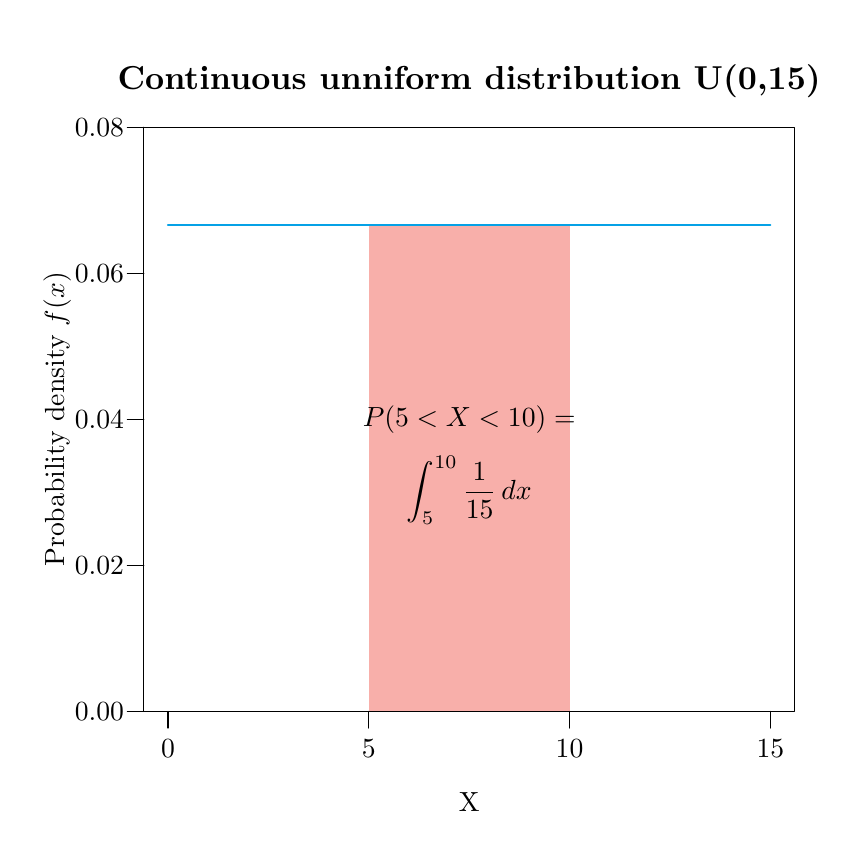
\begin{tikzpicture}[x=1pt,y=1pt]
\definecolor{fillColor}{RGB}{255,255,255}
\path[use as bounding box,fill=fillColor,fill opacity=0.00] (0,0) rectangle (289.08,289.08);
\begin{scope}
\path[clip] (  0.00,  0.00) rectangle (289.08,289.08);
\definecolor{drawColor}{RGB}{0,0,0}

\path[draw=drawColor,line width= 0.4pt,line join=round,line cap=round] ( 50.71, 42.00) -- (268.37, 42.00);

\path[draw=drawColor,line width= 0.4pt,line join=round,line cap=round] ( 50.71, 42.00) -- ( 50.71, 36.00);

\path[draw=drawColor,line width= 0.4pt,line join=round,line cap=round] (123.26, 42.00) -- (123.26, 36.00);

\path[draw=drawColor,line width= 0.4pt,line join=round,line cap=round] (195.82, 42.00) -- (195.82, 36.00);

\path[draw=drawColor,line width= 0.4pt,line join=round,line cap=round] (268.37, 42.00) -- (268.37, 36.00);

\node[text=drawColor,anchor=base,inner sep=0pt, outer sep=0pt, scale=  1.00] at ( 50.71, 25.20) {0};

\node[text=drawColor,anchor=base,inner sep=0pt, outer sep=0pt, scale=  1.00] at (123.26, 25.20) {5};

\node[text=drawColor,anchor=base,inner sep=0pt, outer sep=0pt, scale=  1.00] at (195.82, 25.20) {10};

\node[text=drawColor,anchor=base,inner sep=0pt, outer sep=0pt, scale=  1.00] at (268.37, 25.20) {15};

\path[draw=drawColor,line width= 0.4pt,line join=round,line cap=round] ( 42.00, 42.00) -- ( 42.00,253.08);

\path[draw=drawColor,line width= 0.4pt,line join=round,line cap=round] ( 42.00, 42.00) -- ( 36.00, 42.00);

\path[draw=drawColor,line width= 0.4pt,line join=round,line cap=round] ( 42.00, 94.77) -- ( 36.00, 94.77);

\path[draw=drawColor,line width= 0.4pt,line join=round,line cap=round] ( 42.00,147.54) -- ( 36.00,147.54);

\path[draw=drawColor,line width= 0.4pt,line join=round,line cap=round] ( 42.00,200.31) -- ( 36.00,200.31);

\path[draw=drawColor,line width= 0.4pt,line join=round,line cap=round] ( 42.00,253.08) -- ( 36.00,253.08);

\node[text=drawColor,anchor=base east,inner sep=0pt, outer sep=0pt, scale=  1.00] at ( 34.80, 38.56) {0.00};

\node[text=drawColor,anchor=base east,inner sep=0pt, outer sep=0pt, scale=  1.00] at ( 34.80, 91.33) {0.02};

\node[text=drawColor,anchor=base east,inner sep=0pt, outer sep=0pt, scale=  1.00] at ( 34.80,144.10) {0.04};

\node[text=drawColor,anchor=base east,inner sep=0pt, outer sep=0pt, scale=  1.00] at ( 34.80,196.87) {0.06};

\node[text=drawColor,anchor=base east,inner sep=0pt, outer sep=0pt, scale=  1.00] at ( 34.80,249.64) {0.08};

\path[draw=drawColor,line width= 0.4pt,line join=round,line cap=round] ( 42.00, 42.00) --
	(277.08, 42.00) --
	(277.08,253.08) --
	( 42.00,253.08) --
	( 42.00, 42.00);
\end{scope}
\begin{scope}
\path[clip] (  0.00,  0.00) rectangle (289.08,289.08);
\definecolor{drawColor}{RGB}{0,0,0}

\node[text=drawColor,anchor=base,inner sep=0pt, outer sep=0pt, scale=  1.20] at (159.54,266.89) {\bfseries Continuous unniform distribution U(0,15)};

\node[text=drawColor,anchor=base,inner sep=0pt, outer sep=0pt, scale=  1.00] at (159.54,  6.00) {X};

\node[text=drawColor,rotate= 90.00,anchor=base,inner sep=0pt, outer sep=0pt, scale=  1.00] at ( 13.20,147.54) {Probability density $f(x)$};
\end{scope}
\begin{scope}
\path[clip] ( 42.00, 42.00) rectangle (277.08,253.08);
\definecolor{fillColor}{RGB}{238,50,36}

\path[fill=fillColor,fill opacity=0.39] (123.26, 42.00) --
	(123.26,217.90) --
	(195.82,217.90) --
	(195.82, 42.00) --
	cycle;
\definecolor{drawColor}{RGB}{5,161,230}

\path[draw=drawColor,line width= 0.8pt,line join=round,line cap=round] ( 50.71,217.90) --
	(123.26,217.90) --
	(195.82,217.90) --
	(268.37,217.90);
\definecolor{drawColor}{RGB}{0,0,0}

\node[text=drawColor,anchor=base,inner sep=0pt, outer sep=0pt, scale=  1.00] at (159.54,145.04) {$P(5<X<10)=$};

\node[text=drawColor,anchor=base,inner sep=0pt, outer sep=0pt, scale=  1.00] at (159.54,118.65) {$\displaystyle \int_5^{10} \frac{1}{15}\,dx$};
\end{scope}
\end{tikzpicture}
}}
\mode<presentation>{\resizebox{1\textwidth}{!}{% Created by tikzDevice version 0.9 on 2016-04-29 13:16:45
% !TEX encoding = UTF-8 Unicode
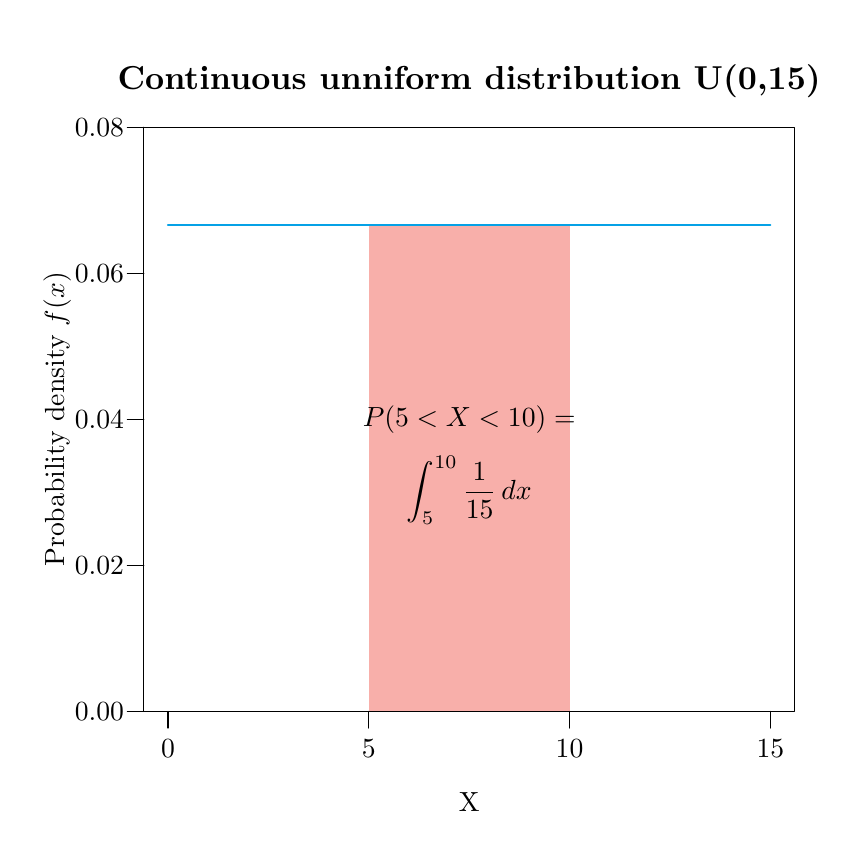
\begin{tikzpicture}[x=1pt,y=1pt]
\definecolor{fillColor}{RGB}{255,255,255}
\path[use as bounding box,fill=fillColor,fill opacity=0.00] (0,0) rectangle (289.08,289.08);
\begin{scope}
\path[clip] (  0.00,  0.00) rectangle (289.08,289.08);
\definecolor{drawColor}{RGB}{0,0,0}

\path[draw=drawColor,line width= 0.4pt,line join=round,line cap=round] ( 50.71, 42.00) -- (268.37, 42.00);

\path[draw=drawColor,line width= 0.4pt,line join=round,line cap=round] ( 50.71, 42.00) -- ( 50.71, 36.00);

\path[draw=drawColor,line width= 0.4pt,line join=round,line cap=round] (123.26, 42.00) -- (123.26, 36.00);

\path[draw=drawColor,line width= 0.4pt,line join=round,line cap=round] (195.82, 42.00) -- (195.82, 36.00);

\path[draw=drawColor,line width= 0.4pt,line join=round,line cap=round] (268.37, 42.00) -- (268.37, 36.00);

\node[text=drawColor,anchor=base,inner sep=0pt, outer sep=0pt, scale=  1.00] at ( 50.71, 25.20) {0};

\node[text=drawColor,anchor=base,inner sep=0pt, outer sep=0pt, scale=  1.00] at (123.26, 25.20) {5};

\node[text=drawColor,anchor=base,inner sep=0pt, outer sep=0pt, scale=  1.00] at (195.82, 25.20) {10};

\node[text=drawColor,anchor=base,inner sep=0pt, outer sep=0pt, scale=  1.00] at (268.37, 25.20) {15};

\path[draw=drawColor,line width= 0.4pt,line join=round,line cap=round] ( 42.00, 42.00) -- ( 42.00,253.08);

\path[draw=drawColor,line width= 0.4pt,line join=round,line cap=round] ( 42.00, 42.00) -- ( 36.00, 42.00);

\path[draw=drawColor,line width= 0.4pt,line join=round,line cap=round] ( 42.00, 94.77) -- ( 36.00, 94.77);

\path[draw=drawColor,line width= 0.4pt,line join=round,line cap=round] ( 42.00,147.54) -- ( 36.00,147.54);

\path[draw=drawColor,line width= 0.4pt,line join=round,line cap=round] ( 42.00,200.31) -- ( 36.00,200.31);

\path[draw=drawColor,line width= 0.4pt,line join=round,line cap=round] ( 42.00,253.08) -- ( 36.00,253.08);

\node[text=drawColor,anchor=base east,inner sep=0pt, outer sep=0pt, scale=  1.00] at ( 34.80, 38.56) {0.00};

\node[text=drawColor,anchor=base east,inner sep=0pt, outer sep=0pt, scale=  1.00] at ( 34.80, 91.33) {0.02};

\node[text=drawColor,anchor=base east,inner sep=0pt, outer sep=0pt, scale=  1.00] at ( 34.80,144.10) {0.04};

\node[text=drawColor,anchor=base east,inner sep=0pt, outer sep=0pt, scale=  1.00] at ( 34.80,196.87) {0.06};

\node[text=drawColor,anchor=base east,inner sep=0pt, outer sep=0pt, scale=  1.00] at ( 34.80,249.64) {0.08};

\path[draw=drawColor,line width= 0.4pt,line join=round,line cap=round] ( 42.00, 42.00) --
	(277.08, 42.00) --
	(277.08,253.08) --
	( 42.00,253.08) --
	( 42.00, 42.00);
\end{scope}
\begin{scope}
\path[clip] (  0.00,  0.00) rectangle (289.08,289.08);
\definecolor{drawColor}{RGB}{0,0,0}

\node[text=drawColor,anchor=base,inner sep=0pt, outer sep=0pt, scale=  1.20] at (159.54,266.89) {\bfseries Continuous unniform distribution U(0,15)};

\node[text=drawColor,anchor=base,inner sep=0pt, outer sep=0pt, scale=  1.00] at (159.54,  6.00) {X};

\node[text=drawColor,rotate= 90.00,anchor=base,inner sep=0pt, outer sep=0pt, scale=  1.00] at ( 13.20,147.54) {Probability density $f(x)$};
\end{scope}
\begin{scope}
\path[clip] ( 42.00, 42.00) rectangle (277.08,253.08);
\definecolor{fillColor}{RGB}{238,50,36}

\path[fill=fillColor,fill opacity=0.39] (123.26, 42.00) --
	(123.26,217.90) --
	(195.82,217.90) --
	(195.82, 42.00) --
	cycle;
\definecolor{drawColor}{RGB}{5,161,230}

\path[draw=drawColor,line width= 0.8pt,line join=round,line cap=round] ( 50.71,217.90) --
	(123.26,217.90) --
	(195.82,217.90) --
	(268.37,217.90);
\definecolor{drawColor}{RGB}{0,0,0}

\node[text=drawColor,anchor=base,inner sep=0pt, outer sep=0pt, scale=  1.00] at (159.54,145.04) {$P(5<X<10)=$};

\node[text=drawColor,anchor=base,inner sep=0pt, outer sep=0pt, scale=  1.00] at (159.54,118.65) {$\displaystyle \int_5^{10} \frac{1}{15}\,dx$};
\end{scope}
\end{tikzpicture}
}}
\end{center}
\end{column}
\end{columns}
And the expected waiting (the mean) time is $\mu=\frac{0+15}{2}=7.5$ minutes.
\end{frame}


\subsection{Normal distribution}

%---------------------------------------------------------------------slide----
\begin{frame}
\frametitle{Normal probability distribution model $N(\mu,\sigma)$}
The normal distribution model is, without a doubt, the most important continuous distribution model as it is the most common in Nature.

\begin{definition}[Normal distribution $N(\mu,\sigma)$]
A continuous random variable $X$ follows a probability distribution model \emph{normal} of parameters $\mu$ and
$\sigma$, noted $X\sim N(\mu,\sigma)$, if its range is $\mbox{Ran}(X) = (-\infty,\infty)$ and its density function is
\[
f(x)= \frac{1}{\sigma\sqrt{2\pi}}e^{-\frac{(x-\mu)^2}{2\sigma^2}}.
\]
\end{definition}

The two parameters $\mu$ and $\sigma$ are the mean and the standard deviation of the population respectively. 
\end{frame}


%---------------------------------------------------------------------slide----
\begin{frame}
\frametitle{Normal Densidad de probabilidad function}
The plot of the Densidad de probabilidad function of a normal distribution $N(\mu,\sigma)$ is bell shaped and it is known as a \emph{Gauss bell}.
\begin{center}
\tikzsetnextfilename{continuous_random_variables/normal_density_function}
\mode<article>{\resizebox{0.6\textwidth}{!}{\input{img/continuous_random_variables/normal_density_function}}}
\mode<presentation>{\resizebox{0.6\textwidth}{!}{\input{img/continuous_random_variables/normal_density_function}}}
\end{center}
\end{frame}


%---------------------------------------------------------------------slide----
\begin{frame}
\frametitle{Normal Densidad de probabilidad function}
The bell shape depends on the mean $\mu$ and the standard deviation $\sigma$,
\begin{itemize}
\item The mean $\mu$ sets the center of the bell.
\item The standard deviation sets $\sigma$ the width of the bell.
\end{itemize}
\medskip
\begin{columns}
\begin{column}{0.47\textwidth}

\mode<presentation>{\resizebox{\textwidth}{!}{% Created by tikzDevice version 0.10.1 on 2016-05-08 18:26:47
% !TEX encoding = UTF-8 Unicode
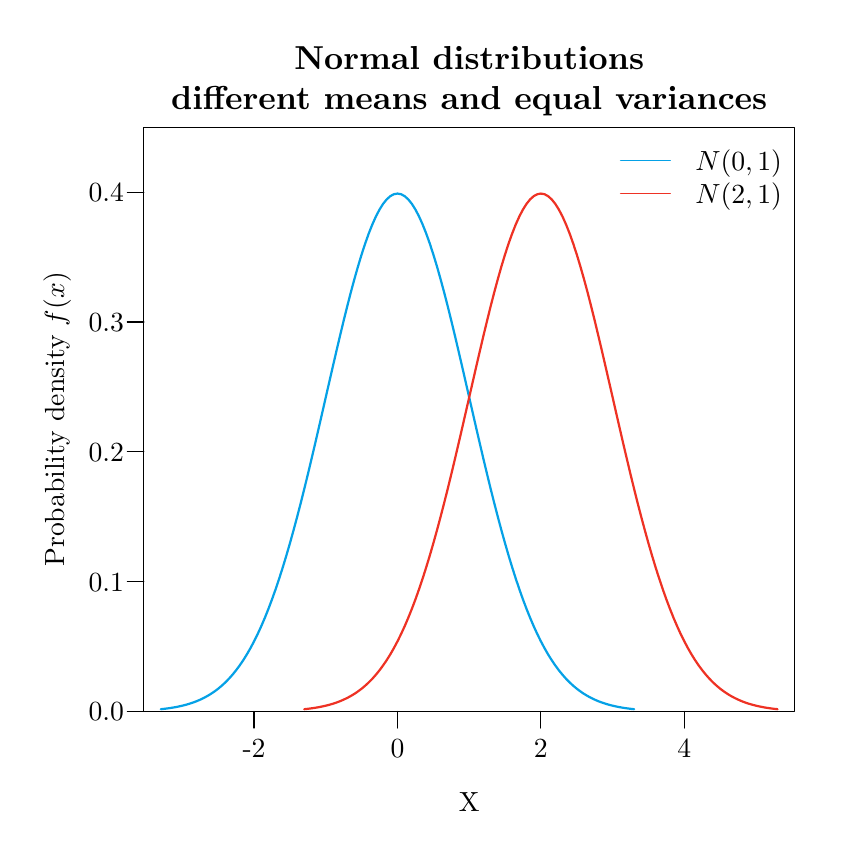
\begin{tikzpicture}[x=1pt,y=1pt]
\definecolor{fillColor}{RGB}{255,255,255}
\path[use as bounding box,fill=fillColor,fill opacity=0.00] (0,0) rectangle (289.08,289.08);
\begin{scope}
\path[clip] ( 42.00, 42.00) rectangle (277.08,253.08);
\definecolor{drawColor}{RGB}{5,161,230}

\path[draw=drawColor,line width= 0.8pt,line join=round,line cap=round] ( 48.12, 42.81) --
	( 49.41, 42.95) --
	( 50.71, 43.12) --
	( 52.00, 43.31) --
	( 53.30, 43.53) --
	( 54.59, 43.79) --
	( 55.89, 44.08) --
	( 57.18, 44.41) --
	( 58.48, 44.79) --
	( 59.78, 45.22) --
	( 61.07, 45.71) --
	( 62.37, 46.27) --
	( 63.66, 46.89) --
	( 64.96, 47.59) --
	( 66.25, 48.37) --
	( 67.55, 49.25) --
	( 68.85, 50.22) --
	( 70.14, 51.31) --
	( 71.44, 52.50) --
	( 72.73, 53.83) --
	( 74.03, 55.29) --
	( 75.32, 56.89) --
	( 76.62, 58.64) --
	( 77.92, 60.55) --
	( 79.21, 62.63) --
	( 80.51, 64.89) --
	( 81.80, 67.33) --
	( 83.10, 69.95) --
	( 84.39, 72.78) --
	( 85.69, 75.80) --
	( 86.98, 79.03) --
	( 88.28, 82.47) --
	( 89.58, 86.12) --
	( 90.87, 89.97) --
	( 92.17, 94.03) --
	( 93.46, 98.29) --
	( 94.76,102.75) --
	( 96.05,107.40) --
	( 97.35,112.23) --
	( 98.65,117.23) --
	( 99.94,122.38) --
	(101.24,127.67) --
	(102.53,133.09) --
	(103.83,138.60) --
	(105.12,144.19) --
	(106.42,149.83) --
	(107.71,155.50) --
	(109.01,161.17) --
	(110.31,166.81) --
	(111.60,172.39) --
	(112.90,177.88) --
	(114.19,183.25) --
	(115.49,188.47) --
	(116.78,193.50) --
	(118.08,198.30) --
	(119.38,202.86) --
	(120.67,207.14) --
	(121.97,211.11) --
	(123.26,214.74) --
	(124.56,218.01) --
	(125.85,220.90) --
	(127.15,223.37) --
	(128.44,225.43) --
	(129.74,227.04) --
	(131.04,228.20) --
	(132.33,228.90) --
	(133.63,229.13) --
	(134.92,228.90) --
	(136.22,228.20) --
	(137.51,227.04) --
	(138.81,225.43) --
	(140.11,223.37) --
	(141.40,220.90) --
	(142.70,218.01) --
	(143.99,214.74) --
	(145.29,211.11) --
	(146.58,207.14) --
	(147.88,202.86) --
	(149.17,198.30) --
	(150.47,193.50) --
	(151.77,188.47) --
	(153.06,183.25) --
	(154.36,177.88) --
	(155.65,172.39) --
	(156.95,166.81) --
	(158.24,161.17) --
	(159.54,155.50) --
	(160.84,149.83) --
	(162.13,144.19) --
	(163.43,138.60) --
	(164.72,133.09) --
	(166.02,127.67) --
	(167.31,122.38) --
	(168.61,117.23) --
	(169.91,112.23) --
	(171.20,107.40) --
	(172.50,102.75) --
	(173.79, 98.29) --
	(175.09, 94.03) --
	(176.38, 89.97) --
	(177.68, 86.12) --
	(178.97, 82.47) --
	(180.27, 79.03) --
	(181.57, 75.80) --
	(182.86, 72.78) --
	(184.16, 69.95) --
	(185.45, 67.33) --
	(186.75, 64.89) --
	(188.04, 62.63) --
	(189.34, 60.55) --
	(190.64, 58.64) --
	(191.93, 56.89) --
	(193.23, 55.29) --
	(194.52, 53.83) --
	(195.82, 52.50) --
	(197.11, 51.31) --
	(198.41, 50.22) --
	(199.70, 49.25) --
	(201.00, 48.37) --
	(202.30, 47.59) --
	(203.59, 46.89) --
	(204.89, 46.27) --
	(206.18, 45.71) --
	(207.48, 45.22) --
	(208.77, 44.79) --
	(210.07, 44.41) --
	(211.37, 44.08) --
	(212.66, 43.79) --
	(213.96, 43.53) --
	(215.25, 43.31) --
	(216.55, 43.12) --
	(217.84, 42.95) --
	(219.14, 42.81);
\end{scope}
\begin{scope}
\path[clip] (  0.00,  0.00) rectangle (289.08,289.08);
\definecolor{drawColor}{RGB}{0,0,0}

\path[draw=drawColor,line width= 0.4pt,line join=round,line cap=round] ( 81.80, 42.00) -- (237.28, 42.00);

\path[draw=drawColor,line width= 0.4pt,line join=round,line cap=round] ( 81.80, 42.00) -- ( 81.80, 36.00);

\path[draw=drawColor,line width= 0.4pt,line join=round,line cap=round] (133.63, 42.00) -- (133.63, 36.00);

\path[draw=drawColor,line width= 0.4pt,line join=round,line cap=round] (185.45, 42.00) -- (185.45, 36.00);

\path[draw=drawColor,line width= 0.4pt,line join=round,line cap=round] (237.28, 42.00) -- (237.28, 36.00);

\node[text=drawColor,anchor=base,inner sep=0pt, outer sep=0pt, scale=  1.00] at ( 81.80, 25.20) {-2};

\node[text=drawColor,anchor=base,inner sep=0pt, outer sep=0pt, scale=  1.00] at (133.63, 25.20) {0};

\node[text=drawColor,anchor=base,inner sep=0pt, outer sep=0pt, scale=  1.00] at (185.45, 25.20) {2};

\node[text=drawColor,anchor=base,inner sep=0pt, outer sep=0pt, scale=  1.00] at (237.28, 25.20) {4};

\path[draw=drawColor,line width= 0.4pt,line join=round,line cap=round] ( 42.00, 42.00) -- ( 42.00,229.63);

\path[draw=drawColor,line width= 0.4pt,line join=round,line cap=round] ( 42.00, 42.00) -- ( 36.00, 42.00);

\path[draw=drawColor,line width= 0.4pt,line join=round,line cap=round] ( 42.00, 88.91) -- ( 36.00, 88.91);

\path[draw=drawColor,line width= 0.4pt,line join=round,line cap=round] ( 42.00,135.81) -- ( 36.00,135.81);

\path[draw=drawColor,line width= 0.4pt,line join=round,line cap=round] ( 42.00,182.72) -- ( 36.00,182.72);

\path[draw=drawColor,line width= 0.4pt,line join=round,line cap=round] ( 42.00,229.63) -- ( 36.00,229.63);

\node[text=drawColor,anchor=base east,inner sep=0pt, outer sep=0pt, scale=  1.00] at ( 34.80, 38.56) {0.0};

\node[text=drawColor,anchor=base east,inner sep=0pt, outer sep=0pt, scale=  1.00] at ( 34.80, 85.46) {0.1};

\node[text=drawColor,anchor=base east,inner sep=0pt, outer sep=0pt, scale=  1.00] at ( 34.80,132.37) {0.2};

\node[text=drawColor,anchor=base east,inner sep=0pt, outer sep=0pt, scale=  1.00] at ( 34.80,179.28) {0.3};

\node[text=drawColor,anchor=base east,inner sep=0pt, outer sep=0pt, scale=  1.00] at ( 34.80,226.18) {0.4};

\path[draw=drawColor,line width= 0.4pt,line join=round,line cap=round] ( 42.00, 42.00) --
	(277.08, 42.00) --
	(277.08,253.08) --
	( 42.00,253.08) --
	( 42.00, 42.00);
\end{scope}
\begin{scope}
\path[clip] (  0.00,  0.00) rectangle (289.08,289.08);
\definecolor{drawColor}{RGB}{0,0,0}

\node[text=drawColor,anchor=base,inner sep=0pt, outer sep=0pt, scale=  1.20] at (159.54,274.09) {\bfseries Normal distributions};

\node[text=drawColor,anchor=base,inner sep=0pt, outer sep=0pt, scale=  1.20] at (159.54,259.69) {\bfseries  different means and equal variances};

\node[text=drawColor,anchor=base,inner sep=0pt, outer sep=0pt, scale=  1.00] at (159.54,  6.00) {X};

\node[text=drawColor,rotate= 90.00,anchor=base,inner sep=0pt, outer sep=0pt, scale=  1.00] at ( 13.20,147.54) {Probability density $f(x)$};
\end{scope}
\begin{scope}
\path[clip] ( 42.00, 42.00) rectangle (277.08,253.08);
\definecolor{drawColor}{RGB}{238,50,36}

\path[draw=drawColor,line width= 0.8pt,line join=round,line cap=round] ( 99.94, 42.81) --
	(101.24, 42.95) --
	(102.53, 43.12) --
	(103.83, 43.31) --
	(105.12, 43.53) --
	(106.42, 43.79) --
	(107.71, 44.08) --
	(109.01, 44.41) --
	(110.31, 44.79) --
	(111.60, 45.22) --
	(112.90, 45.71) --
	(114.19, 46.27) --
	(115.49, 46.89) --
	(116.78, 47.59) --
	(118.08, 48.37) --
	(119.38, 49.25) --
	(120.67, 50.22) --
	(121.97, 51.31) --
	(123.26, 52.50) --
	(124.56, 53.83) --
	(125.85, 55.29) --
	(127.15, 56.89) --
	(128.44, 58.64) --
	(129.74, 60.55) --
	(131.04, 62.63) --
	(132.33, 64.89) --
	(133.63, 67.33) --
	(134.92, 69.95) --
	(136.22, 72.78) --
	(137.51, 75.80) --
	(138.81, 79.03) --
	(140.11, 82.47) --
	(141.40, 86.12) --
	(142.70, 89.97) --
	(143.99, 94.03) --
	(145.29, 98.29) --
	(146.58,102.75) --
	(147.88,107.40) --
	(149.17,112.23) --
	(150.47,117.23) --
	(151.77,122.38) --
	(153.06,127.67) --
	(154.36,133.09) --
	(155.65,138.60) --
	(156.95,144.19) --
	(158.24,149.83) --
	(159.54,155.50) --
	(160.84,161.17) --
	(162.13,166.81) --
	(163.43,172.39) --
	(164.72,177.88) --
	(166.02,183.25) --
	(167.31,188.47) --
	(168.61,193.50) --
	(169.91,198.30) --
	(171.20,202.86) --
	(172.50,207.14) --
	(173.79,211.11) --
	(175.09,214.74) --
	(176.38,218.01) --
	(177.68,220.90) --
	(178.97,223.37) --
	(180.27,225.43) --
	(181.57,227.04) --
	(182.86,228.20) --
	(184.16,228.90) --
	(185.45,229.13) --
	(186.75,228.90) --
	(188.04,228.20) --
	(189.34,227.04) --
	(190.64,225.43) --
	(191.93,223.37) --
	(193.23,220.90) --
	(194.52,218.01) --
	(195.82,214.74) --
	(197.11,211.11) --
	(198.41,207.14) --
	(199.70,202.86) --
	(201.00,198.30) --
	(202.30,193.50) --
	(203.59,188.47) --
	(204.89,183.25) --
	(206.18,177.88) --
	(207.48,172.39) --
	(208.77,166.81) --
	(210.07,161.17) --
	(211.37,155.50) --
	(212.66,149.83) --
	(213.96,144.19) --
	(215.25,138.60) --
	(216.55,133.09) --
	(217.84,127.67) --
	(219.14,122.38) --
	(220.43,117.23) --
	(221.73,112.23) --
	(223.03,107.40) --
	(224.32,102.75) --
	(225.62, 98.29) --
	(226.91, 94.03) --
	(228.21, 89.97) --
	(229.50, 86.12) --
	(230.80, 82.47) --
	(232.10, 79.03) --
	(233.39, 75.80) --
	(234.69, 72.78) --
	(235.98, 69.95) --
	(237.28, 67.33) --
	(238.57, 64.89) --
	(239.87, 62.63) --
	(241.16, 60.55) --
	(242.46, 58.64) --
	(243.76, 56.89) --
	(245.05, 55.29) --
	(246.35, 53.83) --
	(247.64, 52.50) --
	(248.94, 51.31) --
	(250.23, 50.22) --
	(251.53, 49.25) --
	(252.83, 48.37) --
	(254.12, 47.59) --
	(255.42, 46.89) --
	(256.71, 46.27) --
	(258.01, 45.71) --
	(259.30, 45.22) --
	(260.60, 44.79) --
	(261.90, 44.41) --
	(263.19, 44.08) --
	(264.49, 43.79) --
	(265.78, 43.53) --
	(267.08, 43.31) --
	(268.37, 43.12) --
	(269.67, 42.95) --
	(270.96, 42.81);
\definecolor{drawColor}{RGB}{5,161,230}

\path[draw=drawColor,line width= 0.4pt,line join=round,line cap=round] (214.23,241.08) -- (232.23,241.08);
\definecolor{drawColor}{RGB}{238,50,36}

\path[draw=drawColor,line width= 0.4pt,line join=round,line cap=round] (214.23,229.08) -- (232.23,229.08);
\definecolor{drawColor}{RGB}{0,0,0}

\node[text=drawColor,anchor=base west,inner sep=0pt, outer sep=0pt, scale=  1.00] at (241.23,237.64) {$N(0,1)$};

\node[text=drawColor,anchor=base west,inner sep=0pt, outer sep=0pt, scale=  1.00] at (241.23,225.64) {$N(2,1)$};
\end{scope}
\end{tikzpicture}
}}
\end{column}
\begin{column}{0.47\textwidth}
\mode<article>{
\tikzsetnextfilename{continuous_random_variables/normal_density_function_different_means}
\resizebox{0.5\textwidth}{!}{% Created by tikzDevice version 0.10.1 on 2016-05-08 18:26:47
% !TEX encoding = UTF-8 Unicode
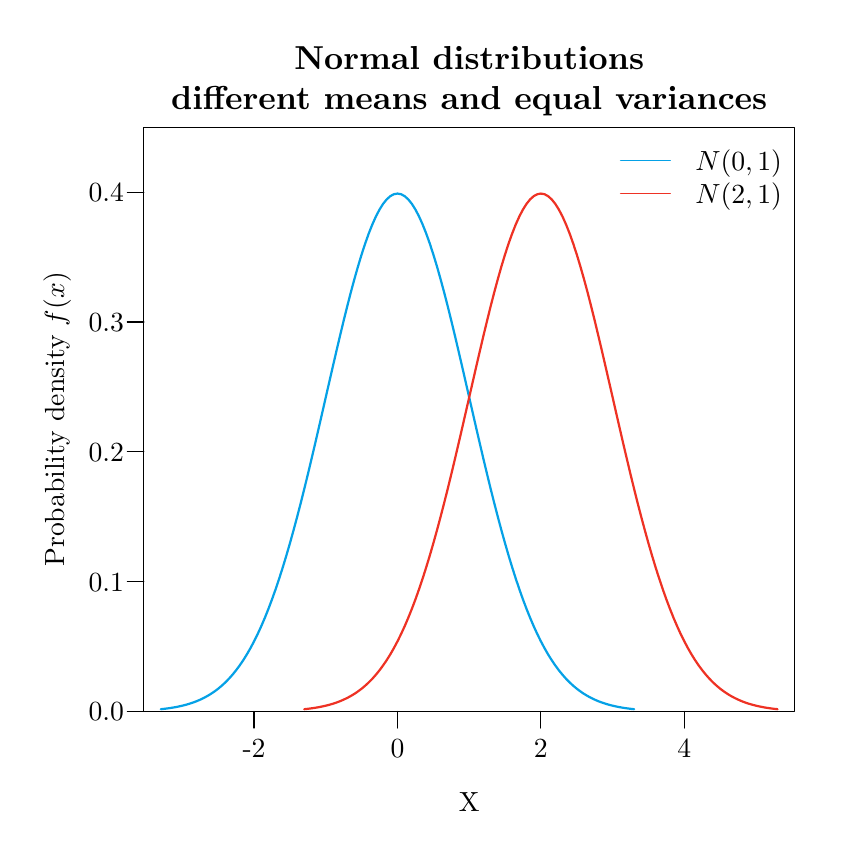
\begin{tikzpicture}[x=1pt,y=1pt]
\definecolor{fillColor}{RGB}{255,255,255}
\path[use as bounding box,fill=fillColor,fill opacity=0.00] (0,0) rectangle (289.08,289.08);
\begin{scope}
\path[clip] ( 42.00, 42.00) rectangle (277.08,253.08);
\definecolor{drawColor}{RGB}{5,161,230}

\path[draw=drawColor,line width= 0.8pt,line join=round,line cap=round] ( 48.12, 42.81) --
	( 49.41, 42.95) --
	( 50.71, 43.12) --
	( 52.00, 43.31) --
	( 53.30, 43.53) --
	( 54.59, 43.79) --
	( 55.89, 44.08) --
	( 57.18, 44.41) --
	( 58.48, 44.79) --
	( 59.78, 45.22) --
	( 61.07, 45.71) --
	( 62.37, 46.27) --
	( 63.66, 46.89) --
	( 64.96, 47.59) --
	( 66.25, 48.37) --
	( 67.55, 49.25) --
	( 68.85, 50.22) --
	( 70.14, 51.31) --
	( 71.44, 52.50) --
	( 72.73, 53.83) --
	( 74.03, 55.29) --
	( 75.32, 56.89) --
	( 76.62, 58.64) --
	( 77.92, 60.55) --
	( 79.21, 62.63) --
	( 80.51, 64.89) --
	( 81.80, 67.33) --
	( 83.10, 69.95) --
	( 84.39, 72.78) --
	( 85.69, 75.80) --
	( 86.98, 79.03) --
	( 88.28, 82.47) --
	( 89.58, 86.12) --
	( 90.87, 89.97) --
	( 92.17, 94.03) --
	( 93.46, 98.29) --
	( 94.76,102.75) --
	( 96.05,107.40) --
	( 97.35,112.23) --
	( 98.65,117.23) --
	( 99.94,122.38) --
	(101.24,127.67) --
	(102.53,133.09) --
	(103.83,138.60) --
	(105.12,144.19) --
	(106.42,149.83) --
	(107.71,155.50) --
	(109.01,161.17) --
	(110.31,166.81) --
	(111.60,172.39) --
	(112.90,177.88) --
	(114.19,183.25) --
	(115.49,188.47) --
	(116.78,193.50) --
	(118.08,198.30) --
	(119.38,202.86) --
	(120.67,207.14) --
	(121.97,211.11) --
	(123.26,214.74) --
	(124.56,218.01) --
	(125.85,220.90) --
	(127.15,223.37) --
	(128.44,225.43) --
	(129.74,227.04) --
	(131.04,228.20) --
	(132.33,228.90) --
	(133.63,229.13) --
	(134.92,228.90) --
	(136.22,228.20) --
	(137.51,227.04) --
	(138.81,225.43) --
	(140.11,223.37) --
	(141.40,220.90) --
	(142.70,218.01) --
	(143.99,214.74) --
	(145.29,211.11) --
	(146.58,207.14) --
	(147.88,202.86) --
	(149.17,198.30) --
	(150.47,193.50) --
	(151.77,188.47) --
	(153.06,183.25) --
	(154.36,177.88) --
	(155.65,172.39) --
	(156.95,166.81) --
	(158.24,161.17) --
	(159.54,155.50) --
	(160.84,149.83) --
	(162.13,144.19) --
	(163.43,138.60) --
	(164.72,133.09) --
	(166.02,127.67) --
	(167.31,122.38) --
	(168.61,117.23) --
	(169.91,112.23) --
	(171.20,107.40) --
	(172.50,102.75) --
	(173.79, 98.29) --
	(175.09, 94.03) --
	(176.38, 89.97) --
	(177.68, 86.12) --
	(178.97, 82.47) --
	(180.27, 79.03) --
	(181.57, 75.80) --
	(182.86, 72.78) --
	(184.16, 69.95) --
	(185.45, 67.33) --
	(186.75, 64.89) --
	(188.04, 62.63) --
	(189.34, 60.55) --
	(190.64, 58.64) --
	(191.93, 56.89) --
	(193.23, 55.29) --
	(194.52, 53.83) --
	(195.82, 52.50) --
	(197.11, 51.31) --
	(198.41, 50.22) --
	(199.70, 49.25) --
	(201.00, 48.37) --
	(202.30, 47.59) --
	(203.59, 46.89) --
	(204.89, 46.27) --
	(206.18, 45.71) --
	(207.48, 45.22) --
	(208.77, 44.79) --
	(210.07, 44.41) --
	(211.37, 44.08) --
	(212.66, 43.79) --
	(213.96, 43.53) --
	(215.25, 43.31) --
	(216.55, 43.12) --
	(217.84, 42.95) --
	(219.14, 42.81);
\end{scope}
\begin{scope}
\path[clip] (  0.00,  0.00) rectangle (289.08,289.08);
\definecolor{drawColor}{RGB}{0,0,0}

\path[draw=drawColor,line width= 0.4pt,line join=round,line cap=round] ( 81.80, 42.00) -- (237.28, 42.00);

\path[draw=drawColor,line width= 0.4pt,line join=round,line cap=round] ( 81.80, 42.00) -- ( 81.80, 36.00);

\path[draw=drawColor,line width= 0.4pt,line join=round,line cap=round] (133.63, 42.00) -- (133.63, 36.00);

\path[draw=drawColor,line width= 0.4pt,line join=round,line cap=round] (185.45, 42.00) -- (185.45, 36.00);

\path[draw=drawColor,line width= 0.4pt,line join=round,line cap=round] (237.28, 42.00) -- (237.28, 36.00);

\node[text=drawColor,anchor=base,inner sep=0pt, outer sep=0pt, scale=  1.00] at ( 81.80, 25.20) {-2};

\node[text=drawColor,anchor=base,inner sep=0pt, outer sep=0pt, scale=  1.00] at (133.63, 25.20) {0};

\node[text=drawColor,anchor=base,inner sep=0pt, outer sep=0pt, scale=  1.00] at (185.45, 25.20) {2};

\node[text=drawColor,anchor=base,inner sep=0pt, outer sep=0pt, scale=  1.00] at (237.28, 25.20) {4};

\path[draw=drawColor,line width= 0.4pt,line join=round,line cap=round] ( 42.00, 42.00) -- ( 42.00,229.63);

\path[draw=drawColor,line width= 0.4pt,line join=round,line cap=round] ( 42.00, 42.00) -- ( 36.00, 42.00);

\path[draw=drawColor,line width= 0.4pt,line join=round,line cap=round] ( 42.00, 88.91) -- ( 36.00, 88.91);

\path[draw=drawColor,line width= 0.4pt,line join=round,line cap=round] ( 42.00,135.81) -- ( 36.00,135.81);

\path[draw=drawColor,line width= 0.4pt,line join=round,line cap=round] ( 42.00,182.72) -- ( 36.00,182.72);

\path[draw=drawColor,line width= 0.4pt,line join=round,line cap=round] ( 42.00,229.63) -- ( 36.00,229.63);

\node[text=drawColor,anchor=base east,inner sep=0pt, outer sep=0pt, scale=  1.00] at ( 34.80, 38.56) {0.0};

\node[text=drawColor,anchor=base east,inner sep=0pt, outer sep=0pt, scale=  1.00] at ( 34.80, 85.46) {0.1};

\node[text=drawColor,anchor=base east,inner sep=0pt, outer sep=0pt, scale=  1.00] at ( 34.80,132.37) {0.2};

\node[text=drawColor,anchor=base east,inner sep=0pt, outer sep=0pt, scale=  1.00] at ( 34.80,179.28) {0.3};

\node[text=drawColor,anchor=base east,inner sep=0pt, outer sep=0pt, scale=  1.00] at ( 34.80,226.18) {0.4};

\path[draw=drawColor,line width= 0.4pt,line join=round,line cap=round] ( 42.00, 42.00) --
	(277.08, 42.00) --
	(277.08,253.08) --
	( 42.00,253.08) --
	( 42.00, 42.00);
\end{scope}
\begin{scope}
\path[clip] (  0.00,  0.00) rectangle (289.08,289.08);
\definecolor{drawColor}{RGB}{0,0,0}

\node[text=drawColor,anchor=base,inner sep=0pt, outer sep=0pt, scale=  1.20] at (159.54,274.09) {\bfseries Normal distributions};

\node[text=drawColor,anchor=base,inner sep=0pt, outer sep=0pt, scale=  1.20] at (159.54,259.69) {\bfseries  different means and equal variances};

\node[text=drawColor,anchor=base,inner sep=0pt, outer sep=0pt, scale=  1.00] at (159.54,  6.00) {X};

\node[text=drawColor,rotate= 90.00,anchor=base,inner sep=0pt, outer sep=0pt, scale=  1.00] at ( 13.20,147.54) {Probability density $f(x)$};
\end{scope}
\begin{scope}
\path[clip] ( 42.00, 42.00) rectangle (277.08,253.08);
\definecolor{drawColor}{RGB}{238,50,36}

\path[draw=drawColor,line width= 0.8pt,line join=round,line cap=round] ( 99.94, 42.81) --
	(101.24, 42.95) --
	(102.53, 43.12) --
	(103.83, 43.31) --
	(105.12, 43.53) --
	(106.42, 43.79) --
	(107.71, 44.08) --
	(109.01, 44.41) --
	(110.31, 44.79) --
	(111.60, 45.22) --
	(112.90, 45.71) --
	(114.19, 46.27) --
	(115.49, 46.89) --
	(116.78, 47.59) --
	(118.08, 48.37) --
	(119.38, 49.25) --
	(120.67, 50.22) --
	(121.97, 51.31) --
	(123.26, 52.50) --
	(124.56, 53.83) --
	(125.85, 55.29) --
	(127.15, 56.89) --
	(128.44, 58.64) --
	(129.74, 60.55) --
	(131.04, 62.63) --
	(132.33, 64.89) --
	(133.63, 67.33) --
	(134.92, 69.95) --
	(136.22, 72.78) --
	(137.51, 75.80) --
	(138.81, 79.03) --
	(140.11, 82.47) --
	(141.40, 86.12) --
	(142.70, 89.97) --
	(143.99, 94.03) --
	(145.29, 98.29) --
	(146.58,102.75) --
	(147.88,107.40) --
	(149.17,112.23) --
	(150.47,117.23) --
	(151.77,122.38) --
	(153.06,127.67) --
	(154.36,133.09) --
	(155.65,138.60) --
	(156.95,144.19) --
	(158.24,149.83) --
	(159.54,155.50) --
	(160.84,161.17) --
	(162.13,166.81) --
	(163.43,172.39) --
	(164.72,177.88) --
	(166.02,183.25) --
	(167.31,188.47) --
	(168.61,193.50) --
	(169.91,198.30) --
	(171.20,202.86) --
	(172.50,207.14) --
	(173.79,211.11) --
	(175.09,214.74) --
	(176.38,218.01) --
	(177.68,220.90) --
	(178.97,223.37) --
	(180.27,225.43) --
	(181.57,227.04) --
	(182.86,228.20) --
	(184.16,228.90) --
	(185.45,229.13) --
	(186.75,228.90) --
	(188.04,228.20) --
	(189.34,227.04) --
	(190.64,225.43) --
	(191.93,223.37) --
	(193.23,220.90) --
	(194.52,218.01) --
	(195.82,214.74) --
	(197.11,211.11) --
	(198.41,207.14) --
	(199.70,202.86) --
	(201.00,198.30) --
	(202.30,193.50) --
	(203.59,188.47) --
	(204.89,183.25) --
	(206.18,177.88) --
	(207.48,172.39) --
	(208.77,166.81) --
	(210.07,161.17) --
	(211.37,155.50) --
	(212.66,149.83) --
	(213.96,144.19) --
	(215.25,138.60) --
	(216.55,133.09) --
	(217.84,127.67) --
	(219.14,122.38) --
	(220.43,117.23) --
	(221.73,112.23) --
	(223.03,107.40) --
	(224.32,102.75) --
	(225.62, 98.29) --
	(226.91, 94.03) --
	(228.21, 89.97) --
	(229.50, 86.12) --
	(230.80, 82.47) --
	(232.10, 79.03) --
	(233.39, 75.80) --
	(234.69, 72.78) --
	(235.98, 69.95) --
	(237.28, 67.33) --
	(238.57, 64.89) --
	(239.87, 62.63) --
	(241.16, 60.55) --
	(242.46, 58.64) --
	(243.76, 56.89) --
	(245.05, 55.29) --
	(246.35, 53.83) --
	(247.64, 52.50) --
	(248.94, 51.31) --
	(250.23, 50.22) --
	(251.53, 49.25) --
	(252.83, 48.37) --
	(254.12, 47.59) --
	(255.42, 46.89) --
	(256.71, 46.27) --
	(258.01, 45.71) --
	(259.30, 45.22) --
	(260.60, 44.79) --
	(261.90, 44.41) --
	(263.19, 44.08) --
	(264.49, 43.79) --
	(265.78, 43.53) --
	(267.08, 43.31) --
	(268.37, 43.12) --
	(269.67, 42.95) --
	(270.96, 42.81);
\definecolor{drawColor}{RGB}{5,161,230}

\path[draw=drawColor,line width= 0.4pt,line join=round,line cap=round] (214.23,241.08) -- (232.23,241.08);
\definecolor{drawColor}{RGB}{238,50,36}

\path[draw=drawColor,line width= 0.4pt,line join=round,line cap=round] (214.23,229.08) -- (232.23,229.08);
\definecolor{drawColor}{RGB}{0,0,0}

\node[text=drawColor,anchor=base west,inner sep=0pt, outer sep=0pt, scale=  1.00] at (241.23,237.64) {$N(0,1)$};

\node[text=drawColor,anchor=base west,inner sep=0pt, outer sep=0pt, scale=  1.00] at (241.23,225.64) {$N(2,1)$};
\end{scope}
\end{tikzpicture}
}
\tikzsetnextfilename{continuous_random_variables/normal_density_function_different_variances}
\resizebox{0.5\textwidth}{!}{% Created by tikzDevice version 0.10.1 on 2016-05-08 18:26:50
% !TEX encoding = UTF-8 Unicode
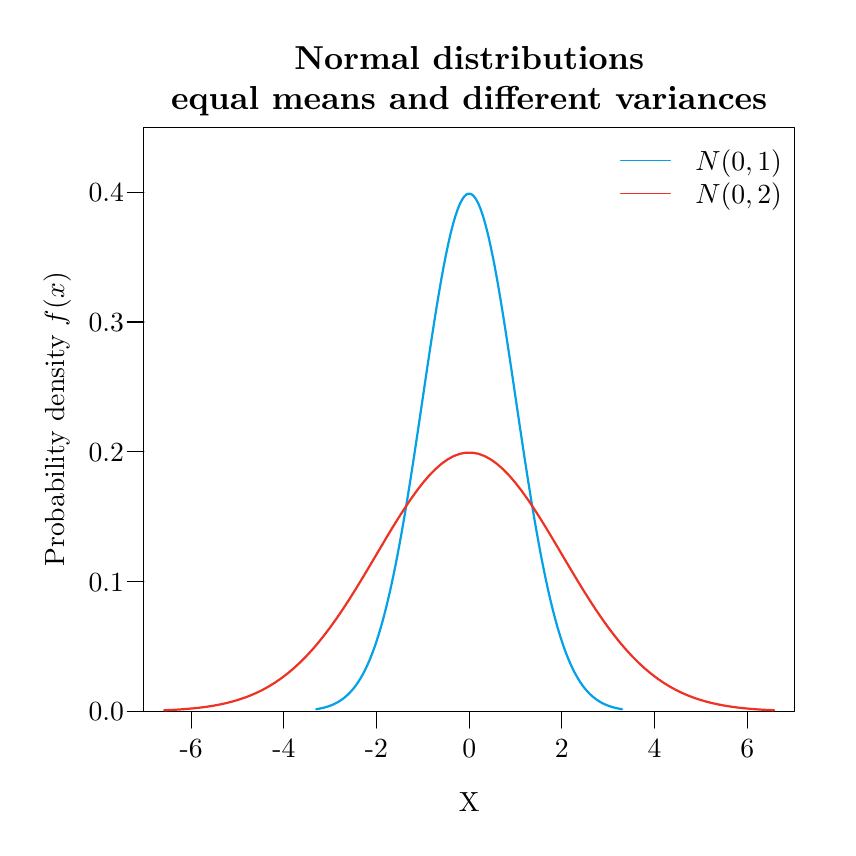
\begin{tikzpicture}[x=1pt,y=1pt]
\definecolor{fillColor}{RGB}{255,255,255}
\path[use as bounding box,fill=fillColor,fill opacity=0.00] (0,0) rectangle (289.08,289.08);
\begin{scope}
\path[clip] ( 42.00, 42.00) rectangle (277.08,253.08);
\definecolor{drawColor}{RGB}{5,161,230}

\path[draw=drawColor,line width= 0.8pt,line join=round,line cap=round] (104.29, 42.81) --
	(105.12, 42.95) --
	(105.96, 43.12) --
	(106.80, 43.31) --
	(107.63, 43.53) --
	(108.47, 43.79) --
	(109.31, 44.08) --
	(110.15, 44.41) --
	(110.98, 44.79) --
	(111.82, 45.22) --
	(112.66, 45.71) --
	(113.50, 46.27) --
	(114.33, 46.89) --
	(115.17, 47.59) --
	(116.01, 48.37) --
	(116.84, 49.25) --
	(117.68, 50.22) --
	(118.52, 51.31) --
	(119.36, 52.50) --
	(120.19, 53.83) --
	(121.03, 55.29) --
	(121.87, 56.89) --
	(122.70, 58.64) --
	(123.54, 60.55) --
	(124.38, 62.63) --
	(125.22, 64.89) --
	(126.05, 67.33) --
	(126.89, 69.95) --
	(127.73, 72.78) --
	(128.56, 75.80) --
	(129.40, 79.03) --
	(130.24, 82.47) --
	(131.08, 86.12) --
	(131.91, 89.97) --
	(132.75, 94.03) --
	(133.59, 98.29) --
	(134.42,102.75) --
	(135.26,107.40) --
	(136.10,112.23) --
	(136.94,117.23) --
	(137.77,122.38) --
	(138.61,127.67) --
	(139.45,133.09) --
	(140.28,138.60) --
	(141.12,144.19) --
	(141.96,149.83) --
	(142.80,155.50) --
	(143.63,161.17) --
	(144.47,166.81) --
	(145.31,172.39) --
	(146.15,177.88) --
	(146.98,183.25) --
	(147.82,188.47) --
	(148.66,193.50) --
	(149.49,198.30) --
	(150.33,202.86) --
	(151.17,207.14) --
	(152.01,211.11) --
	(152.84,214.74) --
	(153.68,218.01) --
	(154.52,220.90) --
	(155.35,223.37) --
	(156.19,225.43) --
	(157.03,227.04) --
	(157.87,228.20) --
	(158.70,228.90) --
	(159.54,229.13) --
	(160.38,228.90) --
	(161.21,228.20) --
	(162.05,227.04) --
	(162.89,225.43) --
	(163.73,223.37) --
	(164.56,220.90) --
	(165.40,218.01) --
	(166.24,214.74) --
	(167.07,211.11) --
	(167.91,207.14) --
	(168.75,202.86) --
	(169.59,198.30) --
	(170.42,193.50) --
	(171.26,188.47) --
	(172.10,183.25) --
	(172.93,177.88) --
	(173.77,172.39) --
	(174.61,166.81) --
	(175.45,161.17) --
	(176.28,155.50) --
	(177.12,149.83) --
	(177.96,144.19) --
	(178.80,138.60) --
	(179.63,133.09) --
	(180.47,127.67) --
	(181.31,122.38) --
	(182.14,117.23) --
	(182.98,112.23) --
	(183.82,107.40) --
	(184.66,102.75) --
	(185.49, 98.29) --
	(186.33, 94.03) --
	(187.17, 89.97) --
	(188.00, 86.12) --
	(188.84, 82.47) --
	(189.68, 79.03) --
	(190.52, 75.80) --
	(191.35, 72.78) --
	(192.19, 69.95) --
	(193.03, 67.33) --
	(193.86, 64.89) --
	(194.70, 62.63) --
	(195.54, 60.55) --
	(196.38, 58.64) --
	(197.21, 56.89) --
	(198.05, 55.29) --
	(198.89, 53.83) --
	(199.72, 52.50) --
	(200.56, 51.31) --
	(201.40, 50.22) --
	(202.24, 49.25) --
	(203.07, 48.37) --
	(203.91, 47.59) --
	(204.75, 46.89) --
	(205.58, 46.27) --
	(206.42, 45.71) --
	(207.26, 45.22) --
	(208.10, 44.79) --
	(208.93, 44.41) --
	(209.77, 44.08) --
	(210.61, 43.79) --
	(211.45, 43.53) --
	(212.28, 43.31) --
	(213.12, 43.12) --
	(213.96, 42.95) --
	(214.79, 42.81);
\end{scope}
\begin{scope}
\path[clip] (  0.00,  0.00) rectangle (289.08,289.08);
\definecolor{drawColor}{RGB}{0,0,0}

\path[draw=drawColor,line width= 0.4pt,line join=round,line cap=round] ( 59.08, 42.00) -- (260.00, 42.00);

\path[draw=drawColor,line width= 0.4pt,line join=round,line cap=round] ( 59.08, 42.00) -- ( 59.08, 36.00);

\path[draw=drawColor,line width= 0.4pt,line join=round,line cap=round] ( 92.57, 42.00) -- ( 92.57, 36.00);

\path[draw=drawColor,line width= 0.4pt,line join=round,line cap=round] (126.05, 42.00) -- (126.05, 36.00);

\path[draw=drawColor,line width= 0.4pt,line join=round,line cap=round] (159.54, 42.00) -- (159.54, 36.00);

\path[draw=drawColor,line width= 0.4pt,line join=round,line cap=round] (193.03, 42.00) -- (193.03, 36.00);

\path[draw=drawColor,line width= 0.4pt,line join=round,line cap=round] (226.51, 42.00) -- (226.51, 36.00);

\path[draw=drawColor,line width= 0.4pt,line join=round,line cap=round] (260.00, 42.00) -- (260.00, 36.00);

\node[text=drawColor,anchor=base,inner sep=0pt, outer sep=0pt, scale=  1.00] at ( 59.08, 25.20) {-6};

\node[text=drawColor,anchor=base,inner sep=0pt, outer sep=0pt, scale=  1.00] at ( 92.57, 25.20) {-4};

\node[text=drawColor,anchor=base,inner sep=0pt, outer sep=0pt, scale=  1.00] at (126.05, 25.20) {-2};

\node[text=drawColor,anchor=base,inner sep=0pt, outer sep=0pt, scale=  1.00] at (159.54, 25.20) {0};

\node[text=drawColor,anchor=base,inner sep=0pt, outer sep=0pt, scale=  1.00] at (193.03, 25.20) {2};

\node[text=drawColor,anchor=base,inner sep=0pt, outer sep=0pt, scale=  1.00] at (226.51, 25.20) {4};

\node[text=drawColor,anchor=base,inner sep=0pt, outer sep=0pt, scale=  1.00] at (260.00, 25.20) {6};

\path[draw=drawColor,line width= 0.4pt,line join=round,line cap=round] ( 42.00, 42.00) -- ( 42.00,229.63);

\path[draw=drawColor,line width= 0.4pt,line join=round,line cap=round] ( 42.00, 42.00) -- ( 36.00, 42.00);

\path[draw=drawColor,line width= 0.4pt,line join=round,line cap=round] ( 42.00, 88.91) -- ( 36.00, 88.91);

\path[draw=drawColor,line width= 0.4pt,line join=round,line cap=round] ( 42.00,135.81) -- ( 36.00,135.81);

\path[draw=drawColor,line width= 0.4pt,line join=round,line cap=round] ( 42.00,182.72) -- ( 36.00,182.72);

\path[draw=drawColor,line width= 0.4pt,line join=round,line cap=round] ( 42.00,229.63) -- ( 36.00,229.63);

\node[text=drawColor,anchor=base east,inner sep=0pt, outer sep=0pt, scale=  1.00] at ( 34.80, 38.56) {0.0};

\node[text=drawColor,anchor=base east,inner sep=0pt, outer sep=0pt, scale=  1.00] at ( 34.80, 85.46) {0.1};

\node[text=drawColor,anchor=base east,inner sep=0pt, outer sep=0pt, scale=  1.00] at ( 34.80,132.37) {0.2};

\node[text=drawColor,anchor=base east,inner sep=0pt, outer sep=0pt, scale=  1.00] at ( 34.80,179.28) {0.3};

\node[text=drawColor,anchor=base east,inner sep=0pt, outer sep=0pt, scale=  1.00] at ( 34.80,226.18) {0.4};

\path[draw=drawColor,line width= 0.4pt,line join=round,line cap=round] ( 42.00, 42.00) --
	(277.08, 42.00) --
	(277.08,253.08) --
	( 42.00,253.08) --
	( 42.00, 42.00);
\end{scope}
\begin{scope}
\path[clip] (  0.00,  0.00) rectangle (289.08,289.08);
\definecolor{drawColor}{RGB}{0,0,0}

\node[text=drawColor,anchor=base,inner sep=0pt, outer sep=0pt, scale=  1.20] at (159.54,274.09) {\bfseries Normal distributions};

\node[text=drawColor,anchor=base,inner sep=0pt, outer sep=0pt, scale=  1.20] at (159.54,259.69) {\bfseries  equal means and different variances};

\node[text=drawColor,anchor=base,inner sep=0pt, outer sep=0pt, scale=  1.00] at (159.54,  6.00) {X};

\node[text=drawColor,rotate= 90.00,anchor=base,inner sep=0pt, outer sep=0pt, scale=  1.00] at ( 13.20,147.54) {Probability density $f(x)$};
\end{scope}
\begin{scope}
\path[clip] ( 42.00, 42.00) rectangle (277.08,253.08);
\definecolor{drawColor}{RGB}{238,50,36}

\path[draw=drawColor,line width= 0.8pt,line join=round,line cap=round] ( 49.35, 42.42) --
	( 51.58, 42.52) --
	( 53.80, 42.64) --
	( 56.03, 42.79) --
	( 58.25, 42.97) --
	( 60.48, 43.18) --
	( 62.71, 43.43) --
	( 64.93, 43.73) --
	( 67.16, 44.08) --
	( 69.38, 44.50) --
	( 71.61, 44.98) --
	( 73.84, 45.54) --
	( 76.06, 46.19) --
	( 78.29, 46.93) --
	( 80.52, 47.78) --
	( 82.74, 48.75) --
	( 84.97, 49.84) --
	( 87.19, 51.07) --
	( 89.42, 52.45) --
	( 91.65, 53.98) --
	( 93.87, 55.68) --
	( 96.10, 57.55) --
	( 98.32, 59.60) --
	(100.55, 61.83) --
	(102.78, 64.24) --
	(105.00, 66.84) --
	(107.23, 69.62) --
	(109.45, 72.57) --
	(111.68, 75.69) --
	(113.91, 78.97) --
	(116.13, 82.39) --
	(118.36, 85.92) --
	(120.58, 89.56) --
	(122.81, 93.27) --
	(125.04, 97.03) --
	(127.26,100.80) --
	(129.49,104.55) --
	(131.71,108.25) --
	(133.94,111.86) --
	(136.17,115.34) --
	(138.39,118.65) --
	(140.62,121.76) --
	(142.84,124.63) --
	(145.07,127.23) --
	(147.30,129.52) --
	(149.52,131.47) --
	(151.75,133.07) --
	(153.97,134.28) --
	(156.20,135.10) --
	(158.43,135.51) --
	(160.65,135.51) --
	(162.88,135.10) --
	(165.11,134.28) --
	(167.33,133.07) --
	(169.56,131.47) --
	(171.78,129.52) --
	(174.01,127.23) --
	(176.24,124.63) --
	(178.46,121.76) --
	(180.69,118.65) --
	(182.91,115.34) --
	(185.14,111.86) --
	(187.37,108.25) --
	(189.59,104.55) --
	(191.82,100.80) --
	(194.04, 97.03) --
	(196.27, 93.27) --
	(198.50, 89.56) --
	(200.72, 85.92) --
	(202.95, 82.39) --
	(205.17, 78.97) --
	(207.40, 75.69) --
	(209.63, 72.57) --
	(211.85, 69.62) --
	(214.08, 66.84) --
	(216.30, 64.24) --
	(218.53, 61.83) --
	(220.76, 59.60) --
	(222.98, 57.55) --
	(225.21, 55.68) --
	(227.43, 53.98) --
	(229.66, 52.45) --
	(231.89, 51.07) --
	(234.11, 49.84) --
	(236.34, 48.75) --
	(238.56, 47.78) --
	(240.79, 46.93) --
	(243.02, 46.19) --
	(245.24, 45.54) --
	(247.47, 44.98) --
	(249.70, 44.50) --
	(251.92, 44.08) --
	(254.15, 43.73) --
	(256.37, 43.43) --
	(258.60, 43.18) --
	(260.83, 42.97) --
	(263.05, 42.79) --
	(265.28, 42.64) --
	(267.50, 42.52) --
	(269.73, 42.42);
\definecolor{drawColor}{RGB}{5,161,230}

\path[draw=drawColor,line width= 0.4pt,line join=round,line cap=round] (214.23,241.08) -- (232.23,241.08);
\definecolor{drawColor}{RGB}{238,50,36}

\path[draw=drawColor,line width= 0.4pt,line join=round,line cap=round] (214.23,229.08) -- (232.23,229.08);
\definecolor{drawColor}{RGB}{0,0,0}

\node[text=drawColor,anchor=base west,inner sep=0pt, outer sep=0pt, scale=  1.00] at (241.23,237.64) {$N(0,1)$};

\node[text=drawColor,anchor=base west,inner sep=0pt, outer sep=0pt, scale=  1.00] at (241.23,225.64) {$N(0,2)$};
\end{scope}
\end{tikzpicture}
}
}
\mode<presentation>{\resizebox{\textwidth}{!}{% Created by tikzDevice version 0.10.1 on 2016-05-08 18:26:50
% !TEX encoding = UTF-8 Unicode
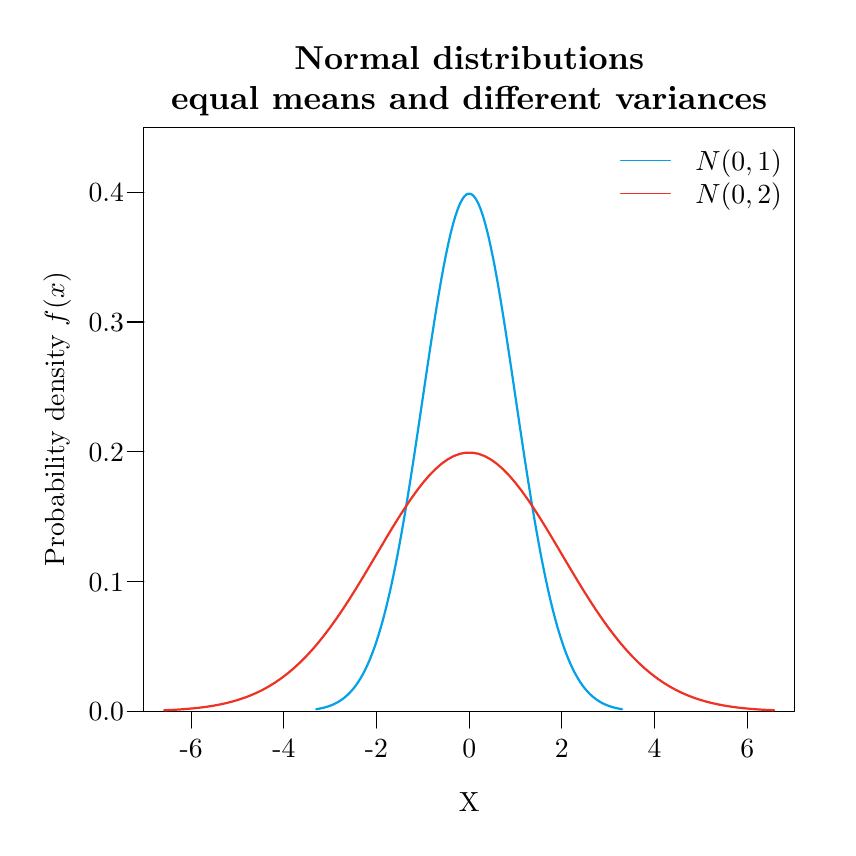
\begin{tikzpicture}[x=1pt,y=1pt]
\definecolor{fillColor}{RGB}{255,255,255}
\path[use as bounding box,fill=fillColor,fill opacity=0.00] (0,0) rectangle (289.08,289.08);
\begin{scope}
\path[clip] ( 42.00, 42.00) rectangle (277.08,253.08);
\definecolor{drawColor}{RGB}{5,161,230}

\path[draw=drawColor,line width= 0.8pt,line join=round,line cap=round] (104.29, 42.81) --
	(105.12, 42.95) --
	(105.96, 43.12) --
	(106.80, 43.31) --
	(107.63, 43.53) --
	(108.47, 43.79) --
	(109.31, 44.08) --
	(110.15, 44.41) --
	(110.98, 44.79) --
	(111.82, 45.22) --
	(112.66, 45.71) --
	(113.50, 46.27) --
	(114.33, 46.89) --
	(115.17, 47.59) --
	(116.01, 48.37) --
	(116.84, 49.25) --
	(117.68, 50.22) --
	(118.52, 51.31) --
	(119.36, 52.50) --
	(120.19, 53.83) --
	(121.03, 55.29) --
	(121.87, 56.89) --
	(122.70, 58.64) --
	(123.54, 60.55) --
	(124.38, 62.63) --
	(125.22, 64.89) --
	(126.05, 67.33) --
	(126.89, 69.95) --
	(127.73, 72.78) --
	(128.56, 75.80) --
	(129.40, 79.03) --
	(130.24, 82.47) --
	(131.08, 86.12) --
	(131.91, 89.97) --
	(132.75, 94.03) --
	(133.59, 98.29) --
	(134.42,102.75) --
	(135.26,107.40) --
	(136.10,112.23) --
	(136.94,117.23) --
	(137.77,122.38) --
	(138.61,127.67) --
	(139.45,133.09) --
	(140.28,138.60) --
	(141.12,144.19) --
	(141.96,149.83) --
	(142.80,155.50) --
	(143.63,161.17) --
	(144.47,166.81) --
	(145.31,172.39) --
	(146.15,177.88) --
	(146.98,183.25) --
	(147.82,188.47) --
	(148.66,193.50) --
	(149.49,198.30) --
	(150.33,202.86) --
	(151.17,207.14) --
	(152.01,211.11) --
	(152.84,214.74) --
	(153.68,218.01) --
	(154.52,220.90) --
	(155.35,223.37) --
	(156.19,225.43) --
	(157.03,227.04) --
	(157.87,228.20) --
	(158.70,228.90) --
	(159.54,229.13) --
	(160.38,228.90) --
	(161.21,228.20) --
	(162.05,227.04) --
	(162.89,225.43) --
	(163.73,223.37) --
	(164.56,220.90) --
	(165.40,218.01) --
	(166.24,214.74) --
	(167.07,211.11) --
	(167.91,207.14) --
	(168.75,202.86) --
	(169.59,198.30) --
	(170.42,193.50) --
	(171.26,188.47) --
	(172.10,183.25) --
	(172.93,177.88) --
	(173.77,172.39) --
	(174.61,166.81) --
	(175.45,161.17) --
	(176.28,155.50) --
	(177.12,149.83) --
	(177.96,144.19) --
	(178.80,138.60) --
	(179.63,133.09) --
	(180.47,127.67) --
	(181.31,122.38) --
	(182.14,117.23) --
	(182.98,112.23) --
	(183.82,107.40) --
	(184.66,102.75) --
	(185.49, 98.29) --
	(186.33, 94.03) --
	(187.17, 89.97) --
	(188.00, 86.12) --
	(188.84, 82.47) --
	(189.68, 79.03) --
	(190.52, 75.80) --
	(191.35, 72.78) --
	(192.19, 69.95) --
	(193.03, 67.33) --
	(193.86, 64.89) --
	(194.70, 62.63) --
	(195.54, 60.55) --
	(196.38, 58.64) --
	(197.21, 56.89) --
	(198.05, 55.29) --
	(198.89, 53.83) --
	(199.72, 52.50) --
	(200.56, 51.31) --
	(201.40, 50.22) --
	(202.24, 49.25) --
	(203.07, 48.37) --
	(203.91, 47.59) --
	(204.75, 46.89) --
	(205.58, 46.27) --
	(206.42, 45.71) --
	(207.26, 45.22) --
	(208.10, 44.79) --
	(208.93, 44.41) --
	(209.77, 44.08) --
	(210.61, 43.79) --
	(211.45, 43.53) --
	(212.28, 43.31) --
	(213.12, 43.12) --
	(213.96, 42.95) --
	(214.79, 42.81);
\end{scope}
\begin{scope}
\path[clip] (  0.00,  0.00) rectangle (289.08,289.08);
\definecolor{drawColor}{RGB}{0,0,0}

\path[draw=drawColor,line width= 0.4pt,line join=round,line cap=round] ( 59.08, 42.00) -- (260.00, 42.00);

\path[draw=drawColor,line width= 0.4pt,line join=round,line cap=round] ( 59.08, 42.00) -- ( 59.08, 36.00);

\path[draw=drawColor,line width= 0.4pt,line join=round,line cap=round] ( 92.57, 42.00) -- ( 92.57, 36.00);

\path[draw=drawColor,line width= 0.4pt,line join=round,line cap=round] (126.05, 42.00) -- (126.05, 36.00);

\path[draw=drawColor,line width= 0.4pt,line join=round,line cap=round] (159.54, 42.00) -- (159.54, 36.00);

\path[draw=drawColor,line width= 0.4pt,line join=round,line cap=round] (193.03, 42.00) -- (193.03, 36.00);

\path[draw=drawColor,line width= 0.4pt,line join=round,line cap=round] (226.51, 42.00) -- (226.51, 36.00);

\path[draw=drawColor,line width= 0.4pt,line join=round,line cap=round] (260.00, 42.00) -- (260.00, 36.00);

\node[text=drawColor,anchor=base,inner sep=0pt, outer sep=0pt, scale=  1.00] at ( 59.08, 25.20) {-6};

\node[text=drawColor,anchor=base,inner sep=0pt, outer sep=0pt, scale=  1.00] at ( 92.57, 25.20) {-4};

\node[text=drawColor,anchor=base,inner sep=0pt, outer sep=0pt, scale=  1.00] at (126.05, 25.20) {-2};

\node[text=drawColor,anchor=base,inner sep=0pt, outer sep=0pt, scale=  1.00] at (159.54, 25.20) {0};

\node[text=drawColor,anchor=base,inner sep=0pt, outer sep=0pt, scale=  1.00] at (193.03, 25.20) {2};

\node[text=drawColor,anchor=base,inner sep=0pt, outer sep=0pt, scale=  1.00] at (226.51, 25.20) {4};

\node[text=drawColor,anchor=base,inner sep=0pt, outer sep=0pt, scale=  1.00] at (260.00, 25.20) {6};

\path[draw=drawColor,line width= 0.4pt,line join=round,line cap=round] ( 42.00, 42.00) -- ( 42.00,229.63);

\path[draw=drawColor,line width= 0.4pt,line join=round,line cap=round] ( 42.00, 42.00) -- ( 36.00, 42.00);

\path[draw=drawColor,line width= 0.4pt,line join=round,line cap=round] ( 42.00, 88.91) -- ( 36.00, 88.91);

\path[draw=drawColor,line width= 0.4pt,line join=round,line cap=round] ( 42.00,135.81) -- ( 36.00,135.81);

\path[draw=drawColor,line width= 0.4pt,line join=round,line cap=round] ( 42.00,182.72) -- ( 36.00,182.72);

\path[draw=drawColor,line width= 0.4pt,line join=round,line cap=round] ( 42.00,229.63) -- ( 36.00,229.63);

\node[text=drawColor,anchor=base east,inner sep=0pt, outer sep=0pt, scale=  1.00] at ( 34.80, 38.56) {0.0};

\node[text=drawColor,anchor=base east,inner sep=0pt, outer sep=0pt, scale=  1.00] at ( 34.80, 85.46) {0.1};

\node[text=drawColor,anchor=base east,inner sep=0pt, outer sep=0pt, scale=  1.00] at ( 34.80,132.37) {0.2};

\node[text=drawColor,anchor=base east,inner sep=0pt, outer sep=0pt, scale=  1.00] at ( 34.80,179.28) {0.3};

\node[text=drawColor,anchor=base east,inner sep=0pt, outer sep=0pt, scale=  1.00] at ( 34.80,226.18) {0.4};

\path[draw=drawColor,line width= 0.4pt,line join=round,line cap=round] ( 42.00, 42.00) --
	(277.08, 42.00) --
	(277.08,253.08) --
	( 42.00,253.08) --
	( 42.00, 42.00);
\end{scope}
\begin{scope}
\path[clip] (  0.00,  0.00) rectangle (289.08,289.08);
\definecolor{drawColor}{RGB}{0,0,0}

\node[text=drawColor,anchor=base,inner sep=0pt, outer sep=0pt, scale=  1.20] at (159.54,274.09) {\bfseries Normal distributions};

\node[text=drawColor,anchor=base,inner sep=0pt, outer sep=0pt, scale=  1.20] at (159.54,259.69) {\bfseries  equal means and different variances};

\node[text=drawColor,anchor=base,inner sep=0pt, outer sep=0pt, scale=  1.00] at (159.54,  6.00) {X};

\node[text=drawColor,rotate= 90.00,anchor=base,inner sep=0pt, outer sep=0pt, scale=  1.00] at ( 13.20,147.54) {Probability density $f(x)$};
\end{scope}
\begin{scope}
\path[clip] ( 42.00, 42.00) rectangle (277.08,253.08);
\definecolor{drawColor}{RGB}{238,50,36}

\path[draw=drawColor,line width= 0.8pt,line join=round,line cap=round] ( 49.35, 42.42) --
	( 51.58, 42.52) --
	( 53.80, 42.64) --
	( 56.03, 42.79) --
	( 58.25, 42.97) --
	( 60.48, 43.18) --
	( 62.71, 43.43) --
	( 64.93, 43.73) --
	( 67.16, 44.08) --
	( 69.38, 44.50) --
	( 71.61, 44.98) --
	( 73.84, 45.54) --
	( 76.06, 46.19) --
	( 78.29, 46.93) --
	( 80.52, 47.78) --
	( 82.74, 48.75) --
	( 84.97, 49.84) --
	( 87.19, 51.07) --
	( 89.42, 52.45) --
	( 91.65, 53.98) --
	( 93.87, 55.68) --
	( 96.10, 57.55) --
	( 98.32, 59.60) --
	(100.55, 61.83) --
	(102.78, 64.24) --
	(105.00, 66.84) --
	(107.23, 69.62) --
	(109.45, 72.57) --
	(111.68, 75.69) --
	(113.91, 78.97) --
	(116.13, 82.39) --
	(118.36, 85.92) --
	(120.58, 89.56) --
	(122.81, 93.27) --
	(125.04, 97.03) --
	(127.26,100.80) --
	(129.49,104.55) --
	(131.71,108.25) --
	(133.94,111.86) --
	(136.17,115.34) --
	(138.39,118.65) --
	(140.62,121.76) --
	(142.84,124.63) --
	(145.07,127.23) --
	(147.30,129.52) --
	(149.52,131.47) --
	(151.75,133.07) --
	(153.97,134.28) --
	(156.20,135.10) --
	(158.43,135.51) --
	(160.65,135.51) --
	(162.88,135.10) --
	(165.11,134.28) --
	(167.33,133.07) --
	(169.56,131.47) --
	(171.78,129.52) --
	(174.01,127.23) --
	(176.24,124.63) --
	(178.46,121.76) --
	(180.69,118.65) --
	(182.91,115.34) --
	(185.14,111.86) --
	(187.37,108.25) --
	(189.59,104.55) --
	(191.82,100.80) --
	(194.04, 97.03) --
	(196.27, 93.27) --
	(198.50, 89.56) --
	(200.72, 85.92) --
	(202.95, 82.39) --
	(205.17, 78.97) --
	(207.40, 75.69) --
	(209.63, 72.57) --
	(211.85, 69.62) --
	(214.08, 66.84) --
	(216.30, 64.24) --
	(218.53, 61.83) --
	(220.76, 59.60) --
	(222.98, 57.55) --
	(225.21, 55.68) --
	(227.43, 53.98) --
	(229.66, 52.45) --
	(231.89, 51.07) --
	(234.11, 49.84) --
	(236.34, 48.75) --
	(238.56, 47.78) --
	(240.79, 46.93) --
	(243.02, 46.19) --
	(245.24, 45.54) --
	(247.47, 44.98) --
	(249.70, 44.50) --
	(251.92, 44.08) --
	(254.15, 43.73) --
	(256.37, 43.43) --
	(258.60, 43.18) --
	(260.83, 42.97) --
	(263.05, 42.79) --
	(265.28, 42.64) --
	(267.50, 42.52) --
	(269.73, 42.42);
\definecolor{drawColor}{RGB}{5,161,230}

\path[draw=drawColor,line width= 0.4pt,line join=round,line cap=round] (214.23,241.08) -- (232.23,241.08);
\definecolor{drawColor}{RGB}{238,50,36}

\path[draw=drawColor,line width= 0.4pt,line join=round,line cap=round] (214.23,229.08) -- (232.23,229.08);
\definecolor{drawColor}{RGB}{0,0,0}

\node[text=drawColor,anchor=base west,inner sep=0pt, outer sep=0pt, scale=  1.00] at (241.23,237.64) {$N(0,1)$};

\node[text=drawColor,anchor=base west,inner sep=0pt, outer sep=0pt, scale=  1.00] at (241.23,225.64) {$N(0,2)$};
\end{scope}
\end{tikzpicture}
}}
\end{column}
\end{columns}
\end{frame}


%---------------------------------------------------------------------slide----
\begin{frame}
\frametitle{Normal distribution function}
The plot of the distribution function of a normal distribution is S shaped. 
\begin{center}
\tikzsetnextfilename{continuous_random_variables/normal_distribution_function}
\mode<article>{\resizebox{0.6\textwidth}{!}{% Created by tikzDevice version 0.10.1 on 2016-05-08 18:26:53
% !TEX encoding = UTF-8 Unicode
\begin{tikzpicture}[x=1pt,y=1pt]
\definecolor{fillColor}{RGB}{255,255,255}
\path[use as bounding box,fill=fillColor,fill opacity=0.00] (0,0) rectangle (289.08,289.08);
\begin{scope}
\path[clip] ( 42.00, 42.00) rectangle (277.08,253.08);
\definecolor{drawColor}{RGB}{5,161,230}

\path[draw=drawColor,line width= 0.8pt,line join=round,line cap=round] ( 50.71, 42.00) --
	( 52.36, 42.02) --
	( 54.00, 42.04) --
	( 55.65, 42.07) --
	( 57.30, 42.10) --
	( 58.95, 42.14) --
	( 60.60, 42.18) --
	( 62.25, 42.23) --
	( 63.90, 42.29) --
	( 65.55, 42.36) --
	( 67.20, 42.44) --
	( 68.85, 42.53) --
	( 70.49, 42.63) --
	( 72.14, 42.75) --
	( 73.79, 42.88) --
	( 75.44, 43.04) --
	( 77.09, 43.21) --
	( 78.74, 43.41) --
	( 80.39, 43.63) --
	( 82.04, 43.88) --
	( 83.69, 44.16) --
	( 85.34, 44.48) --
	( 86.98, 44.84) --
	( 88.63, 45.23) --
	( 90.28, 45.67) --
	( 91.93, 46.16) --
	( 93.58, 46.70) --
	( 95.23, 47.30) --
	( 96.88, 47.97) --
	( 98.53, 48.69) --
	(100.18, 49.49) --
	(101.83, 50.36) --
	(103.47, 51.31) --
	(105.12, 52.35) --
	(106.77, 53.48) --
	(108.42, 54.70) --
	(110.07, 56.01) --
	(111.72, 57.43) --
	(113.37, 58.96) --
	(115.02, 60.60) --
	(116.67, 62.35) --
	(118.32, 64.22) --
	(119.96, 66.21) --
	(121.61, 68.32) --
	(123.26, 70.56) --
	(124.91, 72.93) --
	(126.56, 75.42) --
	(128.21, 78.04) --
	(129.86, 80.79) --
	(131.51, 83.66) --
	(133.16, 86.66) --
	(134.81, 89.78) --
	(136.45, 93.02) --
	(138.10, 96.38) --
	(139.75, 99.84) --
	(141.40,103.42) --
	(143.05,107.09) --
	(144.70,110.85) --
	(146.35,114.70) --
	(148.00,118.63) --
	(149.65,122.63) --
	(151.30,126.68) --
	(152.94,130.79) --
	(154.59,134.94) --
	(156.24,139.13) --
	(157.89,143.33) --
	(159.54,147.54) --
	(161.19,151.75) --
	(162.84,155.95) --
	(164.49,160.14) --
	(166.14,164.29) --
	(167.78,168.40) --
	(169.43,172.45) --
	(171.08,176.45) --
	(172.73,180.38) --
	(174.38,184.23) --
	(176.03,187.99) --
	(177.68,191.66) --
	(179.33,195.24) --
	(180.98,198.70) --
	(182.63,202.06) --
	(184.27,205.30) --
	(185.92,208.42) --
	(187.57,211.42) --
	(189.22,214.29) --
	(190.87,217.04) --
	(192.52,219.66) --
	(194.17,222.15) --
	(195.82,224.52) --
	(197.47,226.76) --
	(199.12,228.87) --
	(200.76,230.86) --
	(202.41,232.73) --
	(204.06,234.48) --
	(205.71,236.12) --
	(207.36,237.65) --
	(209.01,239.07) --
	(210.66,240.38) --
	(212.31,241.60) --
	(213.96,242.73) --
	(215.61,243.77) --
	(217.25,244.72) --
	(218.90,245.59) --
	(220.55,246.39) --
	(222.20,247.11) --
	(223.85,247.78) --
	(225.50,248.38) --
	(227.15,248.92) --
	(228.80,249.41) --
	(230.45,249.85) --
	(232.10,250.24) --
	(233.74,250.60) --
	(235.39,250.92) --
	(237.04,251.20) --
	(238.69,251.45) --
	(240.34,251.67) --
	(241.99,251.87) --
	(243.64,252.04) --
	(245.29,252.20) --
	(246.94,252.33) --
	(248.59,252.45) --
	(250.23,252.55) --
	(251.88,252.64) --
	(253.53,252.72) --
	(255.18,252.79) --
	(256.83,252.85) --
	(258.48,252.90) --
	(260.13,252.94) --
	(261.78,252.98) --
	(263.43,253.01) --
	(265.08,253.04) --
	(266.72,253.06) --
	(268.37,253.08);
\end{scope}
\begin{scope}
\path[clip] (  0.00,  0.00) rectangle (289.08,289.08);
\definecolor{drawColor}{RGB}{0,0,0}

\node[text=drawColor,anchor=base,inner sep=0pt, outer sep=0pt, scale=  1.20] at (159.54,266.89) {\bfseries Normal distribution $N(\mu,\sigma)$};

\node[text=drawColor,anchor=base,inner sep=0pt, outer sep=0pt, scale=  1.00] at (159.54,  6.00) {X};

\node[text=drawColor,rotate= 90.00,anchor=base,inner sep=0pt, outer sep=0pt, scale=  1.00] at ( 13.20,147.54) {Cummulative probability $F(x)$};
\end{scope}
\begin{scope}
\path[clip] (  0.00,  0.00) rectangle (289.08,289.08);
\definecolor{drawColor}{RGB}{0,0,0}

\path[draw=drawColor,line width= 0.4pt,line join=round,line cap=round] (159.54, 42.00) -- (159.54, 42.00);

\path[draw=drawColor,line width= 0.4pt,line join=round,line cap=round] (159.54, 42.00) -- (159.54, 36.00);

\node[text=drawColor,anchor=base,inner sep=0pt, outer sep=0pt, scale=  1.00] at (159.54, 25.20) {$\mu$};

\path[draw=drawColor,line width= 0.4pt,line join=round,line cap=round] ( 42.00, 42.00) --
	(277.08, 42.00) --
	(277.08,253.08) --
	( 42.00,253.08) --
	( 42.00, 42.00);
\end{scope}
\end{tikzpicture}
}}
\mode<presentation>{\resizebox{0.6\textwidth}{!}{% Created by tikzDevice version 0.10.1 on 2016-05-08 18:26:53
% !TEX encoding = UTF-8 Unicode
\begin{tikzpicture}[x=1pt,y=1pt]
\definecolor{fillColor}{RGB}{255,255,255}
\path[use as bounding box,fill=fillColor,fill opacity=0.00] (0,0) rectangle (289.08,289.08);
\begin{scope}
\path[clip] ( 42.00, 42.00) rectangle (277.08,253.08);
\definecolor{drawColor}{RGB}{5,161,230}

\path[draw=drawColor,line width= 0.8pt,line join=round,line cap=round] ( 50.71, 42.00) --
	( 52.36, 42.02) --
	( 54.00, 42.04) --
	( 55.65, 42.07) --
	( 57.30, 42.10) --
	( 58.95, 42.14) --
	( 60.60, 42.18) --
	( 62.25, 42.23) --
	( 63.90, 42.29) --
	( 65.55, 42.36) --
	( 67.20, 42.44) --
	( 68.85, 42.53) --
	( 70.49, 42.63) --
	( 72.14, 42.75) --
	( 73.79, 42.88) --
	( 75.44, 43.04) --
	( 77.09, 43.21) --
	( 78.74, 43.41) --
	( 80.39, 43.63) --
	( 82.04, 43.88) --
	( 83.69, 44.16) --
	( 85.34, 44.48) --
	( 86.98, 44.84) --
	( 88.63, 45.23) --
	( 90.28, 45.67) --
	( 91.93, 46.16) --
	( 93.58, 46.70) --
	( 95.23, 47.30) --
	( 96.88, 47.97) --
	( 98.53, 48.69) --
	(100.18, 49.49) --
	(101.83, 50.36) --
	(103.47, 51.31) --
	(105.12, 52.35) --
	(106.77, 53.48) --
	(108.42, 54.70) --
	(110.07, 56.01) --
	(111.72, 57.43) --
	(113.37, 58.96) --
	(115.02, 60.60) --
	(116.67, 62.35) --
	(118.32, 64.22) --
	(119.96, 66.21) --
	(121.61, 68.32) --
	(123.26, 70.56) --
	(124.91, 72.93) --
	(126.56, 75.42) --
	(128.21, 78.04) --
	(129.86, 80.79) --
	(131.51, 83.66) --
	(133.16, 86.66) --
	(134.81, 89.78) --
	(136.45, 93.02) --
	(138.10, 96.38) --
	(139.75, 99.84) --
	(141.40,103.42) --
	(143.05,107.09) --
	(144.70,110.85) --
	(146.35,114.70) --
	(148.00,118.63) --
	(149.65,122.63) --
	(151.30,126.68) --
	(152.94,130.79) --
	(154.59,134.94) --
	(156.24,139.13) --
	(157.89,143.33) --
	(159.54,147.54) --
	(161.19,151.75) --
	(162.84,155.95) --
	(164.49,160.14) --
	(166.14,164.29) --
	(167.78,168.40) --
	(169.43,172.45) --
	(171.08,176.45) --
	(172.73,180.38) --
	(174.38,184.23) --
	(176.03,187.99) --
	(177.68,191.66) --
	(179.33,195.24) --
	(180.98,198.70) --
	(182.63,202.06) --
	(184.27,205.30) --
	(185.92,208.42) --
	(187.57,211.42) --
	(189.22,214.29) --
	(190.87,217.04) --
	(192.52,219.66) --
	(194.17,222.15) --
	(195.82,224.52) --
	(197.47,226.76) --
	(199.12,228.87) --
	(200.76,230.86) --
	(202.41,232.73) --
	(204.06,234.48) --
	(205.71,236.12) --
	(207.36,237.65) --
	(209.01,239.07) --
	(210.66,240.38) --
	(212.31,241.60) --
	(213.96,242.73) --
	(215.61,243.77) --
	(217.25,244.72) --
	(218.90,245.59) --
	(220.55,246.39) --
	(222.20,247.11) --
	(223.85,247.78) --
	(225.50,248.38) --
	(227.15,248.92) --
	(228.80,249.41) --
	(230.45,249.85) --
	(232.10,250.24) --
	(233.74,250.60) --
	(235.39,250.92) --
	(237.04,251.20) --
	(238.69,251.45) --
	(240.34,251.67) --
	(241.99,251.87) --
	(243.64,252.04) --
	(245.29,252.20) --
	(246.94,252.33) --
	(248.59,252.45) --
	(250.23,252.55) --
	(251.88,252.64) --
	(253.53,252.72) --
	(255.18,252.79) --
	(256.83,252.85) --
	(258.48,252.90) --
	(260.13,252.94) --
	(261.78,252.98) --
	(263.43,253.01) --
	(265.08,253.04) --
	(266.72,253.06) --
	(268.37,253.08);
\end{scope}
\begin{scope}
\path[clip] (  0.00,  0.00) rectangle (289.08,289.08);
\definecolor{drawColor}{RGB}{0,0,0}

\node[text=drawColor,anchor=base,inner sep=0pt, outer sep=0pt, scale=  1.20] at (159.54,266.89) {\bfseries Normal distribution $N(\mu,\sigma)$};

\node[text=drawColor,anchor=base,inner sep=0pt, outer sep=0pt, scale=  1.00] at (159.54,  6.00) {X};

\node[text=drawColor,rotate= 90.00,anchor=base,inner sep=0pt, outer sep=0pt, scale=  1.00] at ( 13.20,147.54) {Cummulative probability $F(x)$};
\end{scope}
\begin{scope}
\path[clip] (  0.00,  0.00) rectangle (289.08,289.08);
\definecolor{drawColor}{RGB}{0,0,0}

\path[draw=drawColor,line width= 0.4pt,line join=round,line cap=round] (159.54, 42.00) -- (159.54, 42.00);

\path[draw=drawColor,line width= 0.4pt,line join=round,line cap=round] (159.54, 42.00) -- (159.54, 36.00);

\node[text=drawColor,anchor=base,inner sep=0pt, outer sep=0pt, scale=  1.00] at (159.54, 25.20) {$\mu$};

\path[draw=drawColor,line width= 0.4pt,line join=round,line cap=round] ( 42.00, 42.00) --
	(277.08, 42.00) --
	(277.08,253.08) --
	( 42.00,253.08) --
	( 42.00, 42.00);
\end{scope}
\end{tikzpicture}
}}
\end{center}
\end{frame}


%---------------------------------------------------------------------slide----
\begin{frame}
\frametitle{Normal distribution properties}
\begin{itemize}
\item It is symmetric with respect to the mean, and therefore, the coefficient of skewness is zero,
$g_1=0$.
\item It is mesokurtic, as the density function is bell shaped, and so, the coefficient of kurtosis is zero, $g_2=0$.
\item The mean, median and mode are the same
\[
\mu = Me = Mo.
\]
\item It asymptotically approaches 0 when $x$ tends to $\pm \infty$.
\end{itemize}
\end{frame}


%---------------------------------------------------------------------slide----
\begin{frame}
\frametitle{Normal distribution properties}
\begin{center}
\onslide<2->{$P(\mu-\sigma \leq X \leq \mu+\sigma) = 0.68$,}\\
\onslide<3->{$P(\mu-2\sigma \leq X \leq \mu+2\sigma) = 0.95$,}\\
\onslide<4->{$P(\mu-3\sigma \leq X \leq \mu+3\sigma) = 0.99$.}
\end{center}

\begin{center}
\mode<article>{
\tikzsetnextfilename{continuous_random_variables/normal_interval_68}
\resizebox{0.33\textwidth}{!}{\input{img/continuous_random_variables/normal_interval_68}
\tikzsetnextfilename{continuous_random_variables/normal_interval_95}}
\resizebox{0.33\textwidth}{!}{\input{img/continuous_random_variables/normal_interval_95}
\tikzsetnextfilename{continuous_random_variables/normal_interval_99}}
\resizebox{0.33\textwidth}{!}{\input{img/continuous_random_variables/normal_interval_99}}
}
\mode<presentation>{\resizebox{0.5\textwidth}{!}{% Created by tikzDevice version 0.10.1 on 2016-05-09 14:41:45
% !TEX encoding = UTF-8 Unicode
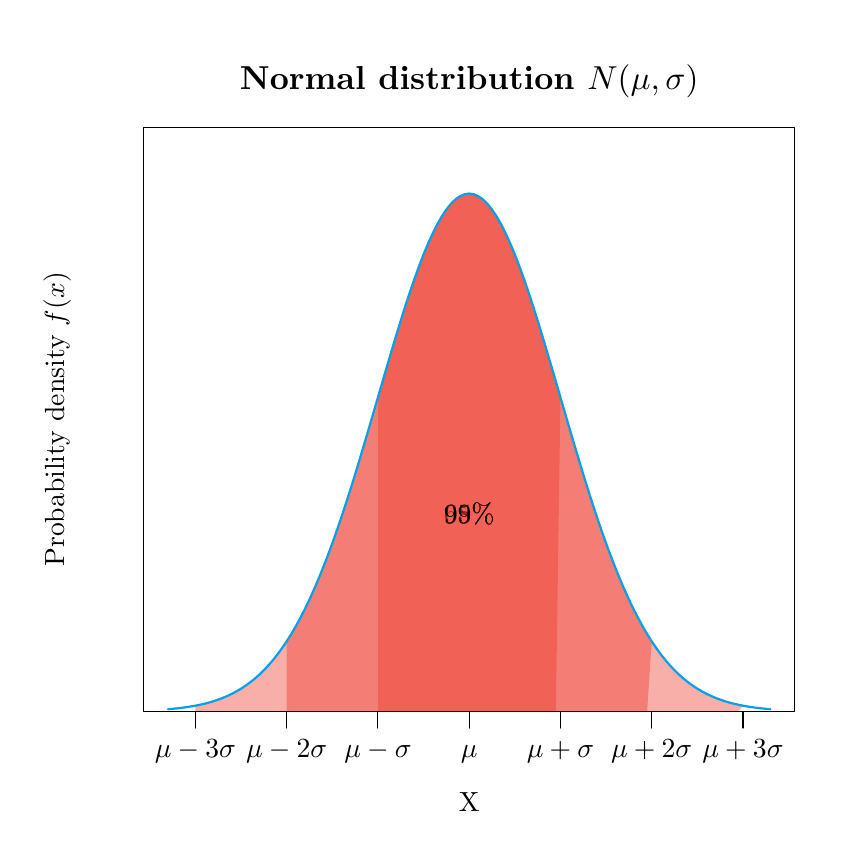
\begin{tikzpicture}[x=1pt,y=1pt]
\definecolor{fillColor}{RGB}{255,255,255}
\path[use as bounding box,fill=fillColor,fill opacity=0.00] (0,0) rectangle (289.08,289.08);
\begin{scope}
\path[clip] (  0.00,  0.00) rectangle (289.08,289.08);
\definecolor{drawColor}{RGB}{0,0,0}

\node[text=drawColor,anchor=base,inner sep=0pt, outer sep=0pt, scale=  1.20] at (159.54,266.89) {\bfseries Normal distribution $N(\mu,\sigma)$};

\node[text=drawColor,anchor=base,inner sep=0pt, outer sep=0pt, scale=  1.00] at (159.54,  6.00) {X};

\node[text=drawColor,rotate= 90.00,anchor=base,inner sep=0pt, outer sep=0pt, scale=  1.00] at ( 13.20,147.54) {Probability density $f(x)$};
\end{scope}
\begin{scope}
\path[clip] (  0.00,  0.00) rectangle (289.08,289.08);
\definecolor{drawColor}{RGB}{0,0,0}

\path[draw=drawColor,line width= 0.4pt,line join=round,line cap=round] (159.54, 42.00) -- (159.54, 42.00);

\path[draw=drawColor,line width= 0.4pt,line join=round,line cap=round] (159.54, 42.00) -- (159.54, 36.00);

\node[text=drawColor,anchor=base,inner sep=0pt, outer sep=0pt, scale=  1.00] at (159.54, 25.20) {$\mu$};

\path[draw=drawColor,line width= 0.4pt,line join=round,line cap=round] (126.56, 42.00) -- (192.52, 42.00);

\onslide<2>{\path[draw=drawColor,line width= 0.4pt,line join=round,line cap=round] (126.56, 42.00) -- (126.56, 36.00);

\path[draw=drawColor,line width= 0.4pt,line join=round,line cap=round] (192.52, 42.00) -- (192.52, 36.00);

\node[text=drawColor,anchor=base,inner sep=0pt, outer sep=0pt, scale=  1.00] at (126.56, 25.20) {$\mu-\sigma$};

\node[text=drawColor,anchor=base,inner sep=0pt, outer sep=0pt, scale=  1.00] at (192.52, 25.20) {$\mu+\sigma$};
}
\end{scope}

\onslide<2>{
\begin{scope}
\path[clip] ( 42.00, 42.00) rectangle (277.08,253.08);
\definecolor{fillColor}{RGB}{238,50,36}

\path[fill=fillColor,fill opacity=0.39] (126.56, 42.00) --
	(126.56,155.50) --
	(128.21,161.17) --
	(129.86,166.81) --
	(131.51,172.39) --
	(133.16,177.88) --
	(134.81,183.25) --
	(136.45,188.47) --
	(138.10,193.50) --
	(139.75,198.30) --
	(141.40,202.86) --
	(143.05,207.14) --
	(144.70,211.11) --
	(146.35,214.74) --
	(148.00,218.01) --
	(149.65,220.90) --
	(151.30,223.37) --
	(152.94,225.43) --
	(154.59,227.04) --
	(156.24,228.20) --
	(157.89,228.90) --
	(159.54,229.13) --
	(161.19,228.90) --
	(162.84,228.20) --
	(164.49,227.04) --
	(166.14,225.43) --
	(167.78,223.37) --
	(169.43,220.90) --
	(171.08,218.01) --
	(172.73,214.74) --
	(174.38,211.11) --
	(176.03,207.14) --
	(177.68,202.86) --
	(179.33,198.30) --
	(180.98,193.50) --
	(182.63,188.47) --
	(184.27,183.25) --
	(185.92,177.88) --
	(187.57,172.39) --
	(189.22,166.81) --
	(190.87,161.17) --
	(192.52,155.50) --
	(190.87, 42.00) --
	cycle;
\definecolor{drawColor}{RGB}{0,0,0}

\node[text=drawColor,anchor=base,inner sep=0pt, outer sep=0pt, scale=  1.00] at (159.54,109.86) {$68\%$};
\end{scope}
}
\onslide<3>{
\begin{scope}
\path[clip] (  0.00,  0.00) rectangle (289.08,289.08);
\definecolor{drawColor}{RGB}{0,0,0}

\path[draw=drawColor,line width= 0.4pt,line join=round,line cap=round] ( 93.58, 42.00) -- (225.50, 42.00);

\path[draw=drawColor,line width= 0.4pt,line join=round,line cap=round] ( 93.58, 42.00) -- ( 93.58, 36.00);

\path[draw=drawColor,line width= 0.4pt,line join=round,line cap=round] (225.50, 42.00) -- (225.50, 36.00);

\node[text=drawColor,anchor=base,inner sep=0pt, outer sep=0pt, scale=  1.00] at ( 93.58, 25.20) {$\mu-2\sigma$};

\node[text=drawColor,anchor=base,inner sep=0pt, outer sep=0pt, scale=  1.00] at (225.50, 25.20) {$\mu+2\sigma$};
\end{scope}
\begin{scope}
\path[clip] ( 42.00, 42.00) rectangle (277.08,253.08);
\definecolor{fillColor}{RGB}{238,50,36}

\path[fill=fillColor,fill opacity=0.39] ( 93.58, 42.00) --
	( 93.58, 67.33) --
	( 95.23, 69.95) --
	( 96.88, 72.78) --
	( 98.53, 75.80) --
	(100.18, 79.03) --
	(101.83, 82.47) --
	(103.47, 86.12) --
	(105.12, 89.97) --
	(106.77, 94.03) --
	(108.42, 98.29) --
	(110.07,102.75) --
	(111.72,107.40) --
	(113.37,112.23) --
	(115.02,117.23) --
	(116.67,122.38) --
	(118.32,127.67) --
	(119.96,133.09) --
	(121.61,138.60) --
	(123.26,144.19) --
	(124.91,149.83) --
	(126.56,155.50) --
	(128.21,161.17) --
	(129.86,166.81) --
	(131.51,172.39) --
	(133.16,177.88) --
	(134.81,183.25) --
	(136.45,188.47) --
	(138.10,193.50) --
	(139.75,198.30) --
	(141.40,202.86) --
	(143.05,207.14) --
	(144.70,211.11) --
	(146.35,214.74) --
	(148.00,218.01) --
	(149.65,220.90) --
	(151.30,223.37) --
	(152.94,225.43) --
	(154.59,227.04) --
	(156.24,228.20) --
	(157.89,228.90) --
	(159.54,229.13) --
	(161.19,228.90) --
	(162.84,228.20) --
	(164.49,227.04) --
	(166.14,225.43) --
	(167.78,223.37) --
	(169.43,220.90) --
	(171.08,218.01) --
	(172.73,214.74) --
	(174.38,211.11) --
	(176.03,207.14) --
	(177.68,202.86) --
	(179.33,198.30) --
	(180.98,193.50) --
	(182.63,188.47) --
	(184.27,183.25) --
	(185.92,177.88) --
	(187.57,172.39) --
	(189.22,166.81) --
	(190.87,161.17) --
	(192.52,155.50) --
	(194.17,149.83) --
	(195.82,144.19) --
	(197.47,138.60) --
	(199.12,133.09) --
	(200.76,127.67) --
	(202.41,122.38) --
	(204.06,117.23) --
	(205.71,112.23) --
	(207.36,107.40) --
	(209.01,102.75) --
	(210.66, 98.29) --
	(212.31, 94.03) --
	(213.96, 89.97) --
	(215.61, 86.12) --
	(217.25, 82.47) --
	(218.90, 79.03) --
	(220.55, 75.80) --
	(222.20, 72.78) --
	(223.85, 69.95) --
	(225.50, 67.33) --
	(223.85, 42.00) --
	cycle;
\definecolor{drawColor}{RGB}{0,0,0}

\node[text=drawColor,anchor=base,inner sep=0pt, outer sep=0pt, scale=  1.00] at (159.54,109.86) {$95\%$};
\end{scope}
}

\onslide<4>{
\begin{scope}
\path[clip] (  0.00,  0.00) rectangle (289.08,289.08);
\definecolor{drawColor}{RGB}{0,0,0}

\path[draw=drawColor,line width= 0.4pt,line join=round,line cap=round] ( 60.60, 42.00) -- (258.48, 42.00);

\path[draw=drawColor,line width= 0.4pt,line join=round,line cap=round] ( 60.60, 42.00) -- ( 60.60, 36.00);

\path[draw=drawColor,line width= 0.4pt,line join=round,line cap=round] (258.48, 42.00) -- (258.48, 36.00);

\node[text=drawColor,anchor=base,inner sep=0pt, outer sep=0pt, scale=  1.00] at ( 60.60, 25.20) {$\mu-3\sigma$};

\node[text=drawColor,anchor=base,inner sep=0pt, outer sep=0pt, scale=  1.00] at (258.48, 25.20) {$\mu+3\sigma$};
\end{scope}
}

\begin{scope}
\path[clip] ( 42.00, 42.00) rectangle (277.08,253.08);
\definecolor{fillColor}{RGB}{238,50,36}
\onslide<4>{
\path[fill=fillColor,fill opacity=0.39] ( 60.60, 42.00) --
	( 60.60, 44.08) --
	( 62.25, 44.41) --
	( 63.90, 44.79) --
	( 65.55, 45.22) --
	( 67.20, 45.71) --
	( 68.85, 46.27) --
	( 70.49, 46.89) --
	( 72.14, 47.59) --
	( 73.79, 48.37) --
	( 75.44, 49.25) --
	( 77.09, 50.22) --
	( 78.74, 51.31) --
	( 80.39, 52.50) --
	( 82.04, 53.83) --
	( 83.69, 55.29) --
	( 85.34, 56.89) --
	( 86.98, 58.64) --
	( 88.63, 60.55) --
	( 90.28, 62.63) --
	( 91.93, 64.89) --
	( 93.58, 67.33) --
	( 95.23, 69.95) --
	( 96.88, 72.78) --
	( 98.53, 75.80) --
	(100.18, 79.03) --
	(101.83, 82.47) --
	(103.47, 86.12) --
	(105.12, 89.97) --
	(106.77, 94.03) --
	(108.42, 98.29) --
	(110.07,102.75) --
	(111.72,107.40) --
	(113.37,112.23) --
	(115.02,117.23) --
	(116.67,122.38) --
	(118.32,127.67) --
	(119.96,133.09) --
	(121.61,138.60) --
	(123.26,144.19) --
	(124.91,149.83) --
	(126.56,155.50) --
	(128.21,161.17) --
	(129.86,166.81) --
	(131.51,172.39) --
	(133.16,177.88) --
	(134.81,183.25) --
	(136.45,188.47) --
	(138.10,193.50) --
	(139.75,198.30) --
	(141.40,202.86) --
	(143.05,207.14) --
	(144.70,211.11) --
	(146.35,214.74) --
	(148.00,218.01) --
	(149.65,220.90) --
	(151.30,223.37) --
	(152.94,225.43) --
	(154.59,227.04) --
	(156.24,228.20) --
	(157.89,228.90) --
	(159.54,229.13) --
	(161.19,228.90) --
	(162.84,228.20) --
	(164.49,227.04) --
	(166.14,225.43) --
	(167.78,223.37) --
	(169.43,220.90) --
	(171.08,218.01) --
	(172.73,214.74) --
	(174.38,211.11) --
	(176.03,207.14) --
	(177.68,202.86) --
	(179.33,198.30) --
	(180.98,193.50) --
	(182.63,188.47) --
	(184.27,183.25) --
	(185.92,177.88) --
	(187.57,172.39) --
	(189.22,166.81) --
	(190.87,161.17) --
	(192.52,155.50) --
	(194.17,149.83) --
	(195.82,144.19) --
	(197.47,138.60) --
	(199.12,133.09) --
	(200.76,127.67) --
	(202.41,122.38) --
	(204.06,117.23) --
	(205.71,112.23) --
	(207.36,107.40) --
	(209.01,102.75) --
	(210.66, 98.29) --
	(212.31, 94.03) --
	(213.96, 89.97) --
	(215.61, 86.12) --
	(217.25, 82.47) --
	(218.90, 79.03) --
	(220.55, 75.80) --
	(222.20, 72.78) --
	(223.85, 69.95) --
	(225.50, 67.33) --
	(227.15, 64.89) --
	(228.80, 62.63) --
	(230.45, 60.55) --
	(232.10, 58.64) --
	(233.74, 56.89) --
	(235.39, 55.29) --
	(237.04, 53.83) --
	(238.69, 52.50) --
	(240.34, 51.31) --
	(241.99, 50.22) --
	(243.64, 49.25) --
	(245.29, 48.37) --
	(246.94, 47.59) --
	(248.59, 46.89) --
	(250.23, 46.27) --
	(251.88, 45.71) --
	(253.53, 45.22) --
	(255.18, 44.79) --
	(256.83, 44.41) --
	(258.48, 44.08) --
	(256.83, 42.00) --
	cycle;
\definecolor{drawColor}{RGB}{0,0,0}

\node[text=drawColor,anchor=base,inner sep=0pt, outer sep=0pt, scale=  1.00] at (159.54,109.86) {$99\%$};
}

\definecolor{drawColor}{RGB}{5,161,230}

\path[draw=drawColor,line width= 0.8pt,line join=round,line cap=round] ( 50.71, 42.81) --
	( 52.36, 42.95) --
	( 54.00, 43.12) --
	( 55.65, 43.31) --
	( 57.30, 43.53) --
	( 58.95, 43.79) --
	( 60.60, 44.08) --
	( 62.25, 44.41) --
	( 63.90, 44.79) --
	( 65.55, 45.22) --
	( 67.20, 45.71) --
	( 68.85, 46.27) --
	( 70.49, 46.89) --
	( 72.14, 47.59) --
	( 73.79, 48.37) --
	( 75.44, 49.25) --
	( 77.09, 50.22) --
	( 78.74, 51.31) --
	( 80.39, 52.50) --
	( 82.04, 53.83) --
	( 83.69, 55.29) --
	( 85.34, 56.89) --
	( 86.98, 58.64) --
	( 88.63, 60.55) --
	( 90.28, 62.63) --
	( 91.93, 64.89) --
	( 93.58, 67.33) --
	( 95.23, 69.95) --
	( 96.88, 72.78) --
	( 98.53, 75.80) --
	(100.18, 79.03) --
	(101.83, 82.47) --
	(103.47, 86.12) --
	(105.12, 89.97) --
	(106.77, 94.03) --
	(108.42, 98.29) --
	(110.07,102.75) --
	(111.72,107.40) --
	(113.37,112.23) --
	(115.02,117.23) --
	(116.67,122.38) --
	(118.32,127.67) --
	(119.96,133.09) --
	(121.61,138.60) --
	(123.26,144.19) --
	(124.91,149.83) --
	(126.56,155.50) --
	(128.21,161.17) --
	(129.86,166.81) --
	(131.51,172.39) --
	(133.16,177.88) --
	(134.81,183.25) --
	(136.45,188.47) --
	(138.10,193.50) --
	(139.75,198.30) --
	(141.40,202.86) --
	(143.05,207.14) --
	(144.70,211.11) --
	(146.35,214.74) --
	(148.00,218.01) --
	(149.65,220.90) --
	(151.30,223.37) --
	(152.94,225.43) --
	(154.59,227.04) --
	(156.24,228.20) --
	(157.89,228.90) --
	(159.54,229.13) --
	(161.19,228.90) --
	(162.84,228.20) --
	(164.49,227.04) --
	(166.14,225.43) --
	(167.78,223.37) --
	(169.43,220.90) --
	(171.08,218.01) --
	(172.73,214.74) --
	(174.38,211.11) --
	(176.03,207.14) --
	(177.68,202.86) --
	(179.33,198.30) --
	(180.98,193.50) --
	(182.63,188.47) --
	(184.27,183.25) --
	(185.92,177.88) --
	(187.57,172.39) --
	(189.22,166.81) --
	(190.87,161.17) --
	(192.52,155.50) --
	(194.17,149.83) --
	(195.82,144.19) --
	(197.47,138.60) --
	(199.12,133.09) --
	(200.76,127.67) --
	(202.41,122.38) --
	(204.06,117.23) --
	(205.71,112.23) --
	(207.36,107.40) --
	(209.01,102.75) --
	(210.66, 98.29) --
	(212.31, 94.03) --
	(213.96, 89.97) --
	(215.61, 86.12) --
	(217.25, 82.47) --
	(218.90, 79.03) --
	(220.55, 75.80) --
	(222.20, 72.78) --
	(223.85, 69.95) --
	(225.50, 67.33) --
	(227.15, 64.89) --
	(228.80, 62.63) --
	(230.45, 60.55) --
	(232.10, 58.64) --
	(233.74, 56.89) --
	(235.39, 55.29) --
	(237.04, 53.83) --
	(238.69, 52.50) --
	(240.34, 51.31) --
	(241.99, 50.22) --
	(243.64, 49.25) --
	(245.29, 48.37) --
	(246.94, 47.59) --
	(248.59, 46.89) --
	(250.23, 46.27) --
	(251.88, 45.71) --
	(253.53, 45.22) --
	(255.18, 44.79) --
	(256.83, 44.41) --
	(258.48, 44.08) --
	(260.13, 43.79) --
	(261.78, 43.53) --
	(263.43, 43.31) --
	(265.08, 43.12) --
	(266.72, 42.95) --
	(268.37, 42.81);
\end{scope}
\begin{scope}
\path[clip] (  0.00,  0.00) rectangle (289.08,289.08);
\definecolor{drawColor}{RGB}{0,0,0}

\path[draw=drawColor,line width= 0.4pt,line join=round,line cap=round] ( 42.00, 42.00) --
	(277.08, 42.00) --
	(277.08,253.08) --
	( 42.00,253.08) --
	( 42.00, 42.00);
\end{scope}
\end{tikzpicture}
}}
\end{center}
\end{frame}


%---------------------------------------------------------------------slide----
\begin{frame}
\frametitle{Normal distribution properties}
\framesubtitle{Example of cholesterol}
It is known that the cholesterol level in females of age between 40 and 50 follows a normal distribution with mean 210 mg/dl and standard deviation 20 mg/dl. 

According to the Gauss bell properties, this means that
\begin{itemize}
\item The 68\% of females have a cholesterol level between $210\pm 20$ mg/dl, i.e., between 190 and 230 mg/dl.
\item The 95\% of females have a cholesterol level between $210\pm 2\cdot 20$ mg/dl, i.e., between  170 and 250 mg/dl.
\item The 99\% of females have a cholesterol level between $210\pm 3\cdot 20$ mg/dl, i.e., between  150 and 270 mg/dl.
\end{itemize}
\end{frame}


%---------------------------------------------------------------------slide----
\begin{frame}
\frametitle{Normal distribution properties}
\framesubtitle{Example blood analysis}
\begin{columns}
\begin{column}{0.47\textwidth}
In blood analysis it is common to use the interval $\mu\pm 2\sigma$ to detect possible pathologies.
In the case of cholesterol, this interval is $[170\text{ mg/dl}, 250\text{ mg/dl}]$. 

Thus, when a women between 40 and 50 years of age has a cholesterol level out of this interval, it's common to think about some pathology.
However this person could be healthy, although the likelihood of that happening is only 5\%.
\end{column}
\begin{column}{0.47\textwidth}
\begin{center}
\mode<article>{\includegraphics[width=0.7\textwidth]{img/continuous_random_variables/blood_analysis.jpg}}
\mode<presentation>{\includegraphics[width=\textwidth]{img/continuous_random_variables/blood_analysis.jpg}}
\end{center}
\end{column}
\end{columns}
\end{frame}


%---------------------------------------------------------------------slide----
\begin{frame}
\frametitle{The central limit theorem}
This behavior is common in many physical and biological variables in Nature.

If you think about the distribution of the height, for instance, you can check that most people in the population have a height around the mean, but as the heights move away from the mean, both below and above the mean, there are few and few people with such a heights.

The explanation for this behavior is the \highlight{\textbf{Central Limit Theorem}}, that we will see in the next
chapter; it states that a continuous random variable whose values depends on a huge number of independent factors adding their effects, always follows a normal distribution.
\end{frame}


%---------------------------------------------------------------------slide----
\begin{frame}
\frametitle{The standard normal distribution $N(0,1)$}
The most important normal distribution has mean zero, $\mu=0$, and standard deviation one, $\sigma=1$.
It is known as \highlight{\textbf{Standard normal distribution}} and usually represented as $Z\sim N(0,1)$.
\begin{center}
\tikzsetnextfilename{continuous_random_variables/standard_normal_density_function}
\mode<article>{\resizebox{0.6\textwidth}{!}{\input{img/continuous_random_variables/standard_normal_density_function}}}
\mode<presentation>{\resizebox{0.55\textwidth}{!}{\input{img/continuous_random_variables/standard_normal_density_function}}}
\end{center}
\end{frame}


%---------------------------------------------------------------------slide----
\begin{frame}
\frametitle{Calculation of probabilities with the standard normal distribution}
\framesubtitle{Managing the distribution function table}
To avoid integrating the normal density function to compute probabilities it's common to use the distribution function,
that is given in a tabular format like the one below.

\begin{columns}
\begin{column}{0.47\textwidth}
\begin{center}
For instance, to calculate $P(Z\leq 0.52)$

\mode<article>{\begin{tabular}[b]
{|r||r|r|r|r|}
\hline
\multicolumn{1}{|c||}{$\mathbf{z}$}& 
\multicolumn{1}{c|}{\textbf{0.00}}& 
\multicolumn{1}{c|}{\textbf{0.01}}& 
\multicolumn{1}{c|}{\highlight{\textbf{0.02}}}& 
\multicolumn{1}{c|}{\textbf{$\cdots$}}\\
\hline\hline
\textbf{0.0}& 
0.5000& 
0.5040& 
0.5080& 
$\cdots$\\
\hline
\textbf{0.1}& 
0.5398& 
0.5438& 
0.5478& 
$\cdots$\\
\hline
\textbf{0.2}& 
0.5793& 
0.5832& 
0.5871& 
$\cdots$\\
\hline
\textbf{0.3}& 
0.6179& 
0.6217& 
0.6255& 
$\cdots$\\
\hline
\textbf{0.4}& 
0.6554& 
0.6591& 
0.6628& 
$\cdots$\\
\hline
\highlight{\textbf{0.5}}& 
0.6915& 
0.6950& 
\cellcolor{color1}{\highlight{\textbf{0.6985}}}& 
$\cdots$\\
\hline
\textbf{$\vdots$}& 
$\vdots$& 
$\vdots$& 
$\vdots$& 
$\ddots$\\
\hline
\end{tabular}}
\mode<presentation>{\scalebox{0.9}{\begin{tabular}[b]
{|r||r|r|r|r|}
\hline
\multicolumn{1}{|c||}{$\mathbf{z}$}& 
\multicolumn{1}{c|}{\textbf{0.00}}& 
\multicolumn{1}{c|}{\textbf{0.01}}& 
\multicolumn{1}{c|}{\highlight{\textbf{0.02}}}& 
\multicolumn{1}{c|}{\textbf{$\cdots$}}\\
\hline\hline
\textbf{0.0}& 
0.5000& 
0.5040& 
0.5080& 
$\cdots$\\
\hline
\textbf{0.1}& 
0.5398& 
0.5438& 
0.5478& 
$\cdots$\\
\hline
\textbf{0.2}& 
0.5793& 
0.5832& 
0.5871& 
$\cdots$\\
\hline
\textbf{0.3}& 
0.6179& 
0.6217& 
0.6255& 
$\cdots$\\
\hline
\textbf{0.4}& 
0.6554& 
0.6591& 
0.6628& 
$\cdots$\\
\hline
\highlight{\textbf{0.5}}& 
0.6915& 
0.6950& 
\cellcolor{color1}{\highlight{\textbf{0.6985}}}& 
$\cdots$\\
\hline
\textbf{$\vdots$}& 
$\vdots$& 
$\vdots$& 
$\vdots$& 
$\ddots$\\
\hline
\end{tabular}}}

$0.52 \rightarrow $ row $0.5$ + column $0.02$
\end{center}
\end{column}
\begin{column}{0.53\textwidth}
\begin{center}
\tikzsetnextfilename{continuous_random_variables/normal_probability_calculation_left_tail}
\mode<article>{\resizebox{0.6\textwidth}{!}{\input{img/continuous_random_variables/normal_probability_calculation_left_tail}}}
\mode<presentation>{\resizebox{0.9\textwidth}{!}{\input{img/continuous_random_variables/normal_probability_calculation_left_tail}}}
\end{center}
\end{column}
\end{columns}
\end{frame}


%---------------------------------------------------------------------slide----
\begin{frame}
\frametitle{Calculation of probabilities with the standard normal distribution}
\framesubtitle{Right tail probabilities}
To compute cumulative probabilities to the right of a value, we can apply the rule for the complement event.
For instance, 
\[
P(Z>0.52) =1-P(Z\leq 0.52) = 1-F(0.52) = 1 - 0.6985 = 0.3015.
\]
\begin{center}
\tikzsetnextfilename{continuous_random_variables/normal_probability_calculation_right_tail}
\mode<article>{\resizebox{0.6\textwidth}{!}{\input{img/continuous_random_variables/normal_probability_calculation_right_tail}}}
\mode<presentation>{\resizebox{0.5\textwidth}{!}{\input{img/continuous_random_variables/normal_probability_calculation_right_tail}}}
\end{center}
\end{frame}


%---------------------------------------------------------------------slide----
\begin{frame}
\frametitle{Standardization}
We have seen how to use the table of the standard normal distribution function to compute probabilities, but, \emph{what to do when the normal distribution is not the standard one?}

In that case we can use standardization to transform any normal distribution in the standard normal distribution.

\begin{theorem}[Standardization]
If $X$ is a continuous random variables that follow a Normal probability distribution model with mean $\mu$ and standard deviation $\sigma$, $X\sim N(\mu,\sigma)$, then the variable that result of subtracting $\mu$ to $X$ and dividing by $\sigma$, follows a Standard Normal probability distribution,
\[
X\sim N(\mu,\sigma) \Rightarrow Z=\frac{X-\mu}{\sigma}\sim N(0,1).
\]
\end{theorem}

Thus, to compute probabilities with a non-standard Normal distribution first we have to standardize the variable before 
using the table of the standard Normal distribution function.
\end{frame}


%---------------------------------------------------------------------slide----
\begin{frame}
\frametitle{Standardization}
\framesubtitle{Example}
Assume that the grade of an exam $X$ follows a Normal probability distribution model $N(\mu=6,\sigma=1.5)$. 
What percentage of students didn't pass the exam?

As $X$ follows a non-standard Normal distribution model, we have to apply standardization first, $Z=\displaystyle
\frac{X-\mu}{\sigma} = \frac{X-6}{1.5}$,
\[
P(X<5) = P\left(\frac{X-6}{1.5}<\frac{5-6}{1.5}\right) = P(Z<-0.67).
\]
Then we can use the table of the standard Normal distribution function,
\[
P(Z<-0.67) = F(-0.67) = 0.2514.
\]

Therefore, $25.14\%$ of students didn't pass the exam.
\end{frame}


\subsection{Chi-square distribution}

%---------------------------------------------------------------------slide----
\begin{frame}
\frametitle{Chi-square probability distribution model $\chi^2(n)$}
\begin{definition}[Chi-square distribution $\chi^2(n)$]
Given $n$ independent random variables $Z_1,\ldots,Z_n$, all of them following a standard normal probability distribution, then the variable
\[
\chi^2(n) = Z_1^2+\cdots +Z_n^2,
\]
follows a \emph{chi-square probability distribution with $n$ degrees of freedom}.
\end{definition}

Its range is $\mathbb{R}^+$ and its mean and variance are
\[
\mu = n, \qquad \sigma^2 = 2n.
\]
As we will see in the next chapter, the chi-square distribution plays an important role in the estimation of the population variance and in the study of relations between qualitative variables.
\end{frame}


%---------------------------------------------------------------------slide----
\begin{frame}
\frametitle{Chi-square Densidad de probabilidad function}

\begin{center}
\tikzsetnextfilename{continuous_random_variables/chi_square_density_function}
\mode<article>{\resizebox{0.6\textwidth}{!}{% Created by tikzDevice version 0.10.1 on 2016-05-08 18:26:05
% !TEX encoding = UTF-8 Unicode
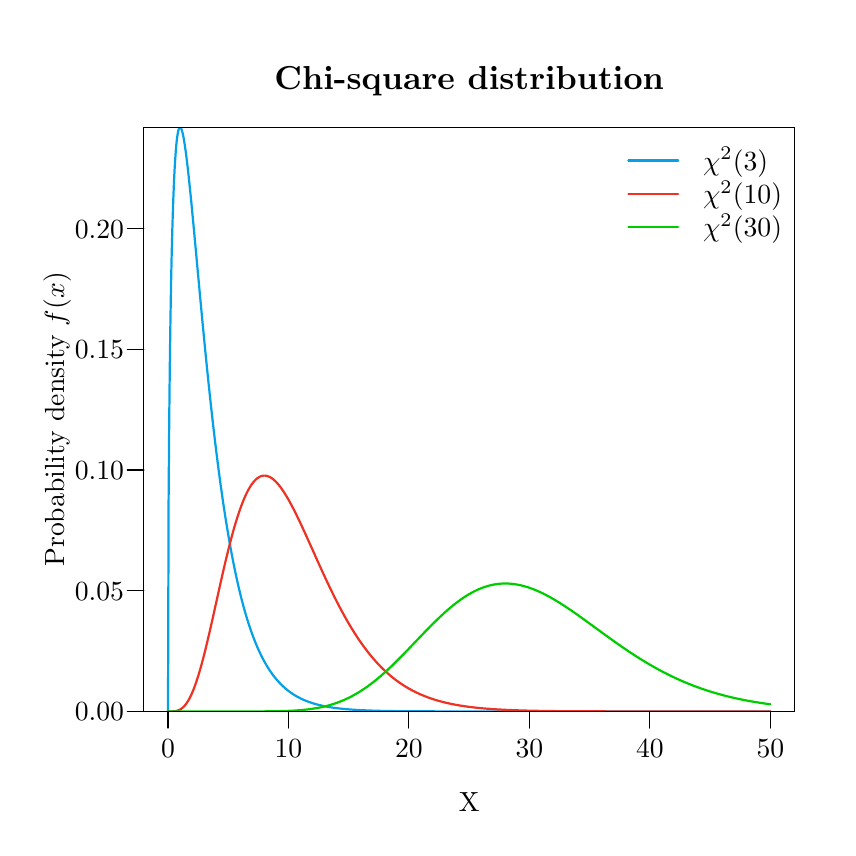
\begin{tikzpicture}[x=1pt,y=1pt]
\definecolor{fillColor}{RGB}{255,255,255}
\path[use as bounding box,fill=fillColor,fill opacity=0.00] (0,0) rectangle (289.08,289.08);
\begin{scope}
\path[clip] ( 42.00, 42.00) rectangle (277.08,253.08);
\definecolor{drawColor}{RGB}{5,161,230}

\path[draw=drawColor,line width= 0.8pt,line join=round,line cap=round] ( 50.71, 42.00) --
	( 50.92,117.90) --
	( 51.14,146.68) --
	( 51.36,167.05) --
	( 51.58,182.83) --
	( 51.79,195.56) --
	( 52.01,206.06) --
	( 52.23,214.83) --
	( 52.45,222.20) --
	( 52.67,228.42) --
	( 52.88,233.65) --
	( 53.10,238.04) --
	( 53.32,241.70) --
	( 53.54,244.72) --
	( 53.75,247.18) --
	( 53.97,249.14) --
	( 54.19,250.65) --
	( 54.41,251.76) --
	( 54.62,252.52) --
	( 54.84,252.94) --
	( 55.06,253.08) --
	( 55.28,252.95) --
	( 55.50,252.59) --
	( 55.71,252.00) --
	( 55.93,251.22) --
	( 56.15,250.26) --
	( 56.37,249.15) --
	( 56.58,247.88) --
	( 56.80,246.48) --
	( 57.02,244.96) --
	( 57.24,243.33) --
	( 57.45,241.61) --
	( 57.67,239.80) --
	( 57.89,237.90) --
	( 58.11,235.94) --
	( 58.32,233.91) --
	( 58.54,231.83) --
	( 58.76,229.70) --
	( 58.98,227.52) --
	( 59.20,225.31) --
	( 59.41,223.06) --
	( 59.63,220.78) --
	( 59.85,218.48) --
	( 60.07,216.16) --
	( 60.28,213.82) --
	( 60.50,211.47) --
	( 60.72,209.12) --
	( 60.94,206.75) --
	( 61.15,204.39) --
	( 61.37,202.02) --
	( 61.59,199.65) --
	( 61.81,197.29) --
	( 62.03,194.93) --
	( 62.24,192.58) --
	( 62.46,190.24) --
	( 62.68,187.92) --
	( 62.90,185.60) --
	( 63.11,183.30) --
	( 63.33,181.02) --
	( 63.55,178.75) --
	( 63.77,176.50) --
	( 63.98,174.27) --
	( 64.20,172.05) --
	( 64.42,169.86) --
	( 64.64,167.69) --
	( 64.85,165.54) --
	( 65.07,163.41) --
	( 65.29,161.31) --
	( 65.51,159.23) --
	( 65.73,157.17) --
	( 65.94,155.14) --
	( 66.16,153.13) --
	( 66.38,151.15) --
	( 66.60,149.19) --
	( 66.81,147.26) --
	( 67.03,145.35) --
	( 67.25,143.47) --
	( 67.47,141.61) --
	( 67.68,139.78) --
	( 67.90,137.98) --
	( 68.12,136.20) --
	( 68.34,134.44) --
	( 68.56,132.72) --
	( 68.77,131.01) --
	( 68.99,129.34) --
	( 69.21,127.69) --
	( 69.43,126.06) --
	( 69.64,124.46) --
	( 69.86,122.89) --
	( 70.08,121.34) --
	( 70.30,119.81) --
	( 70.51,118.31) --
	( 70.73,116.83) --
	( 70.95,115.38) --
	( 71.17,113.95) --
	( 71.38,112.55) --
	( 71.60,111.17) --
	( 71.82,109.81) --
	( 72.04,108.48) --
	( 72.26,107.17) --
	( 72.47,105.88) --
	( 72.69,104.61) --
	( 72.91,103.37) --
	( 73.13,102.14) --
	( 73.34,100.94) --
	( 73.56, 99.76) --
	( 73.78, 98.60) --
	( 74.00, 97.47) --
	( 74.21, 96.35) --
	( 74.43, 95.25) --
	( 74.65, 94.18) --
	( 74.87, 93.12) --
	( 75.09, 92.08) --
	( 75.30, 91.06) --
	( 75.52, 90.06) --
	( 75.74, 89.08) --
	( 75.96, 88.12) --
	( 76.17, 87.17) --
	( 76.39, 86.24) --
	( 76.61, 85.33) --
	( 76.83, 84.44) --
	( 77.04, 83.57) --
	( 77.26, 82.71) --
	( 77.48, 81.86) --
	( 77.70, 81.04) --
	( 77.91, 80.23) --
	( 78.13, 79.43) --
	( 78.35, 78.65) --
	( 78.57, 77.89) --
	( 78.79, 77.14) --
	( 79.00, 76.40) --
	( 79.22, 75.68) --
	( 79.44, 74.98) --
	( 79.66, 74.28) --
	( 79.87, 73.60) --
	( 80.09, 72.94) --
	( 80.31, 72.29) --
	( 80.53, 71.65) --
	( 80.74, 71.02) --
	( 80.96, 70.41) --
	( 81.18, 69.80) --
	( 81.40, 69.21) --
	( 81.62, 68.64) --
	( 81.83, 68.07) --
	( 82.05, 67.52) --
	( 82.27, 66.97) --
	( 82.49, 66.44) --
	( 82.70, 65.92) --
	( 82.92, 65.41) --
	( 83.14, 64.90) --
	( 83.36, 64.41) --
	( 83.57, 63.93) --
	( 83.79, 63.46) --
	( 84.01, 63.00) --
	( 84.23, 62.55) --
	( 84.44, 62.11) --
	( 84.66, 61.67) --
	( 84.88, 61.25) --
	( 85.10, 60.83) --
	( 85.32, 60.43) --
	( 85.53, 60.03) --
	( 85.75, 59.64) --
	( 85.97, 59.26) --
	( 86.19, 58.88) --
	( 86.40, 58.52) --
	( 86.62, 58.16) --
	( 86.84, 57.81) --
	( 87.06, 57.46) --
	( 87.27, 57.13) --
	( 87.49, 56.80) --
	( 87.71, 56.47) --
	( 87.93, 56.16) --
	( 88.15, 55.85) --
	( 88.36, 55.54) --
	( 88.58, 55.25) --
	( 88.80, 54.96) --
	( 89.02, 54.67) --
	( 89.23, 54.40) --
	( 89.45, 54.12) --
	( 89.67, 53.86) --
	( 89.89, 53.60) --
	( 90.10, 53.34) --
	( 90.32, 53.09) --
	( 90.54, 52.85) --
	( 90.76, 52.61) --
	( 90.97, 52.38) --
	( 91.19, 52.15) --
	( 91.41, 51.92) --
	( 91.63, 51.70) --
	( 91.85, 51.49) --
	( 92.06, 51.28) --
	( 92.28, 51.07) --
	( 92.50, 50.87) --
	( 92.72, 50.68) --
	( 92.93, 50.49) --
	( 93.15, 50.30) --
	( 93.37, 50.11) --
	( 93.59, 49.93) --
	( 93.80, 49.76) --
	( 94.02, 49.58) --
	( 94.24, 49.42) --
	( 94.46, 49.25) --
	( 94.68, 49.09) --
	( 94.89, 48.93) --
	( 95.11, 48.78) --
	( 95.33, 48.63) --
	( 95.55, 48.48) --
	( 95.76, 48.33) --
	( 95.98, 48.19) --
	( 96.20, 48.05) --
	( 96.42, 47.92) --
	( 96.63, 47.79) --
	( 96.85, 47.66) --
	( 97.07, 47.53) --
	( 97.29, 47.41) --
	( 97.50, 47.28) --
	( 97.72, 47.17) --
	( 97.94, 47.05) --
	( 98.16, 46.94) --
	( 98.38, 46.83) --
	( 98.59, 46.72) --
	( 98.81, 46.61) --
	( 99.03, 46.51) --
	( 99.25, 46.41) --
	( 99.46, 46.31) --
	( 99.68, 46.21) --
	( 99.90, 46.11) --
	(100.12, 46.02) --
	(100.33, 45.93) --
	(100.55, 45.84) --
	(100.77, 45.76) --
	(100.99, 45.67) --
	(101.21, 45.59) --
	(101.42, 45.51) --
	(101.64, 45.43) --
	(101.86, 45.35) --
	(102.08, 45.27) --
	(102.29, 45.20) --
	(102.51, 45.13) --
	(102.73, 45.06) --
	(102.95, 44.99) --
	(103.16, 44.92) --
	(103.38, 44.85) --
	(103.60, 44.79) --
	(103.82, 44.73) --
	(104.03, 44.66) --
	(104.25, 44.60) --
	(104.47, 44.54) --
	(104.69, 44.49) --
	(104.91, 44.43) --
	(105.12, 44.38) --
	(105.34, 44.32) --
	(105.56, 44.27) --
	(105.78, 44.22) --
	(105.99, 44.17) --
	(106.21, 44.12) --
	(106.43, 44.07) --
	(106.65, 44.02) --
	(106.86, 43.98) --
	(107.08, 43.93) --
	(107.30, 43.89) --
	(107.52, 43.84) --
	(107.74, 43.80) --
	(107.95, 43.76) --
	(108.17, 43.72) --
	(108.39, 43.68) --
	(108.61, 43.64) --
	(108.82, 43.60) --
	(109.04, 43.57) --
	(109.26, 43.53) --
	(109.48, 43.50) --
	(109.69, 43.46) --
	(109.91, 43.43) --
	(110.13, 43.40) --
	(110.35, 43.36) --
	(110.56, 43.33) --
	(110.78, 43.30) --
	(111.00, 43.27) --
	(111.22, 43.24) --
	(111.44, 43.22) --
	(111.65, 43.19) --
	(111.87, 43.16) --
	(112.09, 43.13) --
	(112.31, 43.11) --
	(112.52, 43.08) --
	(112.74, 43.06) --
	(112.96, 43.03) --
	(113.18, 43.01) --
	(113.39, 42.99) --
	(113.61, 42.96) --
	(113.83, 42.94) --
	(114.05, 42.92) --
	(114.27, 42.90) --
	(114.48, 42.88) --
	(114.70, 42.86) --
	(114.92, 42.84) --
	(115.14, 42.82) --
	(115.35, 42.80) --
	(115.57, 42.78) --
	(115.79, 42.76) --
	(116.01, 42.75) --
	(116.22, 42.73) --
	(116.44, 42.71) --
	(116.66, 42.70) --
	(116.88, 42.68) --
	(117.09, 42.66) --
	(117.31, 42.65) --
	(117.53, 42.63) --
	(117.75, 42.62) --
	(117.97, 42.60) --
	(118.18, 42.59) --
	(118.40, 42.58) --
	(118.62, 42.56) --
	(118.84, 42.55) --
	(119.05, 42.54) --
	(119.27, 42.53) --
	(119.49, 42.51) --
	(119.71, 42.50) --
	(119.92, 42.49) --
	(120.14, 42.48) --
	(120.36, 42.47) --
	(120.58, 42.46) --
	(120.80, 42.45) --
	(121.01, 42.44) --
	(121.23, 42.43) --
	(121.45, 42.42) --
	(121.67, 42.41) --
	(121.88, 42.40) --
	(122.10, 42.39) --
	(122.32, 42.38) --
	(122.54, 42.37) --
	(122.75, 42.36) --
	(122.97, 42.35) --
	(123.19, 42.34) --
	(123.41, 42.34) --
	(123.62, 42.33) --
	(123.84, 42.32) --
	(124.06, 42.31) --
	(124.28, 42.31) --
	(124.50, 42.30) --
	(124.71, 42.29) --
	(124.93, 42.29) --
	(125.15, 42.28) --
	(125.37, 42.27) --
	(125.58, 42.27) --
	(125.80, 42.26) --
	(126.02, 42.25) --
	(126.24, 42.25) --
	(126.45, 42.24) --
	(126.67, 42.24) --
	(126.89, 42.23) --
	(127.11, 42.23) --
	(127.33, 42.22) --
	(127.54, 42.21) --
	(127.76, 42.21) --
	(127.98, 42.21) --
	(128.20, 42.20) --
	(128.41, 42.20) --
	(128.63, 42.19) --
	(128.85, 42.19) --
	(129.07, 42.18) --
	(129.28, 42.18) --
	(129.50, 42.17) --
	(129.72, 42.17) --
	(129.94, 42.17) --
	(130.16, 42.16) --
	(130.37, 42.16) --
	(130.59, 42.15) --
	(130.81, 42.15) --
	(131.03, 42.15) --
	(131.24, 42.14) --
	(131.46, 42.14) --
	(131.68, 42.14) --
	(131.90, 42.13) --
	(132.11, 42.13) --
	(132.33, 42.13) --
	(132.55, 42.12) --
	(132.77, 42.12) --
	(132.98, 42.12) --
	(133.20, 42.12) --
	(133.42, 42.11) --
	(133.64, 42.11) --
	(133.86, 42.11) --
	(134.07, 42.11) --
	(134.29, 42.10) --
	(134.51, 42.10) --
	(134.73, 42.10) --
	(134.94, 42.10) --
	(135.16, 42.09) --
	(135.38, 42.09) --
	(135.60, 42.09) --
	(135.81, 42.09) --
	(136.03, 42.09) --
	(136.25, 42.08) --
	(136.47, 42.08) --
	(136.68, 42.08) --
	(136.90, 42.08) --
	(137.12, 42.08) --
	(137.34, 42.07) --
	(137.56, 42.07) --
	(137.77, 42.07) --
	(137.99, 42.07) --
	(138.21, 42.07) --
	(138.43, 42.07) --
	(138.64, 42.06) --
	(138.86, 42.06) --
	(139.08, 42.06) --
	(139.30, 42.06) --
	(139.51, 42.06) --
	(139.73, 42.06) --
	(139.95, 42.06) --
	(140.17, 42.05) --
	(140.39, 42.05) --
	(140.60, 42.05) --
	(140.82, 42.05) --
	(141.04, 42.05) --
	(141.26, 42.05) --
	(141.47, 42.05) --
	(141.69, 42.05) --
	(141.91, 42.04) --
	(142.13, 42.04) --
	(142.34, 42.04) --
	(142.56, 42.04) --
	(142.78, 42.04) --
	(143.00, 42.04) --
	(143.21, 42.04) --
	(143.43, 42.04) --
	(143.65, 42.04) --
	(143.87, 42.04) --
	(144.09, 42.04) --
	(144.30, 42.03) --
	(144.52, 42.03) --
	(144.74, 42.03) --
	(144.96, 42.03) --
	(145.17, 42.03) --
	(145.39, 42.03) --
	(145.61, 42.03) --
	(145.83, 42.03) --
	(146.04, 42.03) --
	(146.26, 42.03) --
	(146.48, 42.03) --
	(146.70, 42.03) --
	(146.92, 42.03) --
	(147.13, 42.03) --
	(147.35, 42.02) --
	(147.57, 42.02) --
	(147.79, 42.02) --
	(148.00, 42.02) --
	(148.22, 42.02) --
	(148.44, 42.02) --
	(148.66, 42.02) --
	(148.87, 42.02) --
	(149.09, 42.02) --
	(149.31, 42.02) --
	(149.53, 42.02) --
	(149.74, 42.02) --
	(149.96, 42.02) --
	(150.18, 42.02) --
	(150.40, 42.02) --
	(150.62, 42.02) --
	(150.83, 42.02) --
	(151.05, 42.02) --
	(151.27, 42.02) --
	(151.49, 42.02) --
	(151.70, 42.02) --
	(151.92, 42.02) --
	(152.14, 42.01) --
	(152.36, 42.01) --
	(152.57, 42.01) --
	(152.79, 42.01) --
	(153.01, 42.01) --
	(153.23, 42.01) --
	(153.45, 42.01) --
	(153.66, 42.01) --
	(153.88, 42.01) --
	(154.10, 42.01) --
	(154.32, 42.01) --
	(154.53, 42.01) --
	(154.75, 42.01) --
	(154.97, 42.01) --
	(155.19, 42.01) --
	(155.40, 42.01) --
	(155.62, 42.01) --
	(155.84, 42.01) --
	(156.06, 42.01) --
	(156.27, 42.01) --
	(156.49, 42.01) --
	(156.71, 42.01) --
	(156.93, 42.01) --
	(157.15, 42.01) --
	(157.36, 42.01) --
	(157.58, 42.01) --
	(157.80, 42.01) --
	(158.02, 42.01) --
	(158.23, 42.01) --
	(158.45, 42.01) --
	(158.67, 42.01) --
	(158.89, 42.01) --
	(159.10, 42.01) --
	(159.32, 42.01) --
	(159.54, 42.01) --
	(159.76, 42.01) --
	(159.98, 42.01) --
	(160.19, 42.01) --
	(160.41, 42.01) --
	(160.63, 42.01) --
	(160.85, 42.01) --
	(161.06, 42.01) --
	(161.28, 42.01) --
	(161.50, 42.01) --
	(161.72, 42.01) --
	(161.93, 42.00) --
	(162.15, 42.00) --
	(162.37, 42.00) --
	(162.59, 42.00) --
	(162.80, 42.00) --
	(163.02, 42.00) --
	(163.24, 42.00) --
	(163.46, 42.00) --
	(163.68, 42.00) --
	(163.89, 42.00) --
	(164.11, 42.00) --
	(164.33, 42.00) --
	(164.55, 42.00) --
	(164.76, 42.00) --
	(164.98, 42.00) --
	(165.20, 42.00) --
	(165.42, 42.00) --
	(165.63, 42.00) --
	(165.85, 42.00) --
	(166.07, 42.00) --
	(166.29, 42.00) --
	(166.51, 42.00) --
	(166.72, 42.00) --
	(166.94, 42.00) --
	(167.16, 42.00) --
	(167.38, 42.00) --
	(167.59, 42.00) --
	(167.81, 42.00) --
	(168.03, 42.00) --
	(168.25, 42.00) --
	(168.46, 42.00) --
	(168.68, 42.00) --
	(168.90, 42.00) --
	(169.12, 42.00) --
	(169.33, 42.00) --
	(169.55, 42.00) --
	(169.77, 42.00) --
	(169.99, 42.00) --
	(170.21, 42.00) --
	(170.42, 42.00) --
	(170.64, 42.00) --
	(170.86, 42.00) --
	(171.08, 42.00) --
	(171.29, 42.00) --
	(171.51, 42.00) --
	(171.73, 42.00) --
	(171.95, 42.00) --
	(172.16, 42.00) --
	(172.38, 42.00) --
	(172.60, 42.00) --
	(172.82, 42.00) --
	(173.04, 42.00) --
	(173.25, 42.00) --
	(173.47, 42.00) --
	(173.69, 42.00) --
	(173.91, 42.00) --
	(174.12, 42.00) --
	(174.34, 42.00) --
	(174.56, 42.00) --
	(174.78, 42.00) --
	(174.99, 42.00) --
	(175.21, 42.00) --
	(175.43, 42.00) --
	(175.65, 42.00) --
	(175.86, 42.00) --
	(176.08, 42.00) --
	(176.30, 42.00) --
	(176.52, 42.00) --
	(176.74, 42.00) --
	(176.95, 42.00) --
	(177.17, 42.00) --
	(177.39, 42.00) --
	(177.61, 42.00) --
	(177.82, 42.00) --
	(178.04, 42.00) --
	(178.26, 42.00) --
	(178.48, 42.00) --
	(178.69, 42.00) --
	(178.91, 42.00) --
	(179.13, 42.00) --
	(179.35, 42.00) --
	(179.57, 42.00) --
	(179.78, 42.00) --
	(180.00, 42.00) --
	(180.22, 42.00) --
	(180.44, 42.00) --
	(180.65, 42.00) --
	(180.87, 42.00) --
	(181.09, 42.00) --
	(181.31, 42.00) --
	(181.52, 42.00) --
	(181.74, 42.00) --
	(181.96, 42.00) --
	(182.18, 42.00) --
	(182.39, 42.00) --
	(182.61, 42.00) --
	(182.83, 42.00) --
	(183.05, 42.00) --
	(183.27, 42.00) --
	(183.48, 42.00) --
	(183.70, 42.00) --
	(183.92, 42.00) --
	(184.14, 42.00) --
	(184.35, 42.00) --
	(184.57, 42.00) --
	(184.79, 42.00) --
	(185.01, 42.00) --
	(185.22, 42.00) --
	(185.44, 42.00) --
	(185.66, 42.00) --
	(185.88, 42.00) --
	(186.10, 42.00) --
	(186.31, 42.00) --
	(186.53, 42.00) --
	(186.75, 42.00) --
	(186.97, 42.00) --
	(187.18, 42.00) --
	(187.40, 42.00) --
	(187.62, 42.00) --
	(187.84, 42.00) --
	(188.05, 42.00) --
	(188.27, 42.00) --
	(188.49, 42.00) --
	(188.71, 42.00) --
	(188.92, 42.00) --
	(189.14, 42.00) --
	(189.36, 42.00) --
	(189.58, 42.00) --
	(189.80, 42.00) --
	(190.01, 42.00) --
	(190.23, 42.00) --
	(190.45, 42.00) --
	(190.67, 42.00) --
	(190.88, 42.00) --
	(191.10, 42.00) --
	(191.32, 42.00) --
	(191.54, 42.00) --
	(191.75, 42.00) --
	(191.97, 42.00) --
	(192.19, 42.00) --
	(192.41, 42.00) --
	(192.63, 42.00) --
	(192.84, 42.00) --
	(193.06, 42.00) --
	(193.28, 42.00) --
	(193.50, 42.00) --
	(193.71, 42.00) --
	(193.93, 42.00) --
	(194.15, 42.00) --
	(194.37, 42.00) --
	(194.58, 42.00) --
	(194.80, 42.00) --
	(195.02, 42.00) --
	(195.24, 42.00) --
	(195.45, 42.00) --
	(195.67, 42.00) --
	(195.89, 42.00) --
	(196.11, 42.00) --
	(196.33, 42.00) --
	(196.54, 42.00) --
	(196.76, 42.00) --
	(196.98, 42.00) --
	(197.20, 42.00) --
	(197.41, 42.00) --
	(197.63, 42.00) --
	(197.85, 42.00) --
	(198.07, 42.00) --
	(198.28, 42.00) --
	(198.50, 42.00) --
	(198.72, 42.00) --
	(198.94, 42.00) --
	(199.16, 42.00) --
	(199.37, 42.00) --
	(199.59, 42.00) --
	(199.81, 42.00) --
	(200.03, 42.00) --
	(200.24, 42.00) --
	(200.46, 42.00) --
	(200.68, 42.00) --
	(200.90, 42.00) --
	(201.11, 42.00) --
	(201.33, 42.00) --
	(201.55, 42.00) --
	(201.77, 42.00) --
	(201.98, 42.00) --
	(202.20, 42.00) --
	(202.42, 42.00) --
	(202.64, 42.00) --
	(202.86, 42.00) --
	(203.07, 42.00) --
	(203.29, 42.00) --
	(203.51, 42.00) --
	(203.73, 42.00) --
	(203.94, 42.00) --
	(204.16, 42.00) --
	(204.38, 42.00) --
	(204.60, 42.00) --
	(204.81, 42.00) --
	(205.03, 42.00) --
	(205.25, 42.00) --
	(205.47, 42.00) --
	(205.69, 42.00) --
	(205.90, 42.00) --
	(206.12, 42.00) --
	(206.34, 42.00) --
	(206.56, 42.00) --
	(206.77, 42.00) --
	(206.99, 42.00) --
	(207.21, 42.00) --
	(207.43, 42.00) --
	(207.64, 42.00) --
	(207.86, 42.00) --
	(208.08, 42.00) --
	(208.30, 42.00) --
	(208.51, 42.00) --
	(208.73, 42.00) --
	(208.95, 42.00) --
	(209.17, 42.00) --
	(209.39, 42.00) --
	(209.60, 42.00) --
	(209.82, 42.00) --
	(210.04, 42.00) --
	(210.26, 42.00) --
	(210.47, 42.00) --
	(210.69, 42.00) --
	(210.91, 42.00) --
	(211.13, 42.00) --
	(211.34, 42.00) --
	(211.56, 42.00) --
	(211.78, 42.00) --
	(212.00, 42.00) --
	(212.22, 42.00) --
	(212.43, 42.00) --
	(212.65, 42.00) --
	(212.87, 42.00) --
	(213.09, 42.00) --
	(213.30, 42.00) --
	(213.52, 42.00) --
	(213.74, 42.00) --
	(213.96, 42.00) --
	(214.17, 42.00) --
	(214.39, 42.00) --
	(214.61, 42.00) --
	(214.83, 42.00) --
	(215.04, 42.00) --
	(215.26, 42.00) --
	(215.48, 42.00) --
	(215.70, 42.00) --
	(215.92, 42.00) --
	(216.13, 42.00) --
	(216.35, 42.00) --
	(216.57, 42.00) --
	(216.79, 42.00) --
	(217.00, 42.00) --
	(217.22, 42.00) --
	(217.44, 42.00) --
	(217.66, 42.00) --
	(217.87, 42.00) --
	(218.09, 42.00) --
	(218.31, 42.00) --
	(218.53, 42.00) --
	(218.75, 42.00) --
	(218.96, 42.00) --
	(219.18, 42.00) --
	(219.40, 42.00) --
	(219.62, 42.00) --
	(219.83, 42.00) --
	(220.05, 42.00) --
	(220.27, 42.00) --
	(220.49, 42.00) --
	(220.70, 42.00) --
	(220.92, 42.00) --
	(221.14, 42.00) --
	(221.36, 42.00) --
	(221.57, 42.00) --
	(221.79, 42.00) --
	(222.01, 42.00) --
	(222.23, 42.00) --
	(222.45, 42.00) --
	(222.66, 42.00) --
	(222.88, 42.00) --
	(223.10, 42.00) --
	(223.32, 42.00) --
	(223.53, 42.00) --
	(223.75, 42.00) --
	(223.97, 42.00) --
	(224.19, 42.00) --
	(224.40, 42.00) --
	(224.62, 42.00) --
	(224.84, 42.00) --
	(225.06, 42.00) --
	(225.28, 42.00) --
	(225.49, 42.00) --
	(225.71, 42.00) --
	(225.93, 42.00) --
	(226.15, 42.00) --
	(226.36, 42.00) --
	(226.58, 42.00) --
	(226.80, 42.00) --
	(227.02, 42.00) --
	(227.23, 42.00) --
	(227.45, 42.00) --
	(227.67, 42.00) --
	(227.89, 42.00) --
	(228.10, 42.00) --
	(228.32, 42.00) --
	(228.54, 42.00) --
	(228.76, 42.00) --
	(228.98, 42.00) --
	(229.19, 42.00) --
	(229.41, 42.00) --
	(229.63, 42.00) --
	(229.85, 42.00) --
	(230.06, 42.00) --
	(230.28, 42.00) --
	(230.50, 42.00) --
	(230.72, 42.00) --
	(230.93, 42.00) --
	(231.15, 42.00) --
	(231.37, 42.00) --
	(231.59, 42.00) --
	(231.81, 42.00) --
	(232.02, 42.00) --
	(232.24, 42.00) --
	(232.46, 42.00) --
	(232.68, 42.00) --
	(232.89, 42.00) --
	(233.11, 42.00) --
	(233.33, 42.00) --
	(233.55, 42.00) --
	(233.76, 42.00) --
	(233.98, 42.00) --
	(234.20, 42.00) --
	(234.42, 42.00) --
	(234.63, 42.00) --
	(234.85, 42.00) --
	(235.07, 42.00) --
	(235.29, 42.00) --
	(235.51, 42.00) --
	(235.72, 42.00) --
	(235.94, 42.00) --
	(236.16, 42.00) --
	(236.38, 42.00) --
	(236.59, 42.00) --
	(236.81, 42.00) --
	(237.03, 42.00) --
	(237.25, 42.00) --
	(237.46, 42.00) --
	(237.68, 42.00) --
	(237.90, 42.00) --
	(238.12, 42.00) --
	(238.34, 42.00) --
	(238.55, 42.00) --
	(238.77, 42.00) --
	(238.99, 42.00) --
	(239.21, 42.00) --
	(239.42, 42.00) --
	(239.64, 42.00) --
	(239.86, 42.00) --
	(240.08, 42.00) --
	(240.29, 42.00) --
	(240.51, 42.00) --
	(240.73, 42.00) --
	(240.95, 42.00) --
	(241.16, 42.00) --
	(241.38, 42.00) --
	(241.60, 42.00) --
	(241.82, 42.00) --
	(242.04, 42.00) --
	(242.25, 42.00) --
	(242.47, 42.00) --
	(242.69, 42.00) --
	(242.91, 42.00) --
	(243.12, 42.00) --
	(243.34, 42.00) --
	(243.56, 42.00) --
	(243.78, 42.00) --
	(243.99, 42.00) --
	(244.21, 42.00) --
	(244.43, 42.00) --
	(244.65, 42.00) --
	(244.87, 42.00) --
	(245.08, 42.00) --
	(245.30, 42.00) --
	(245.52, 42.00) --
	(245.74, 42.00) --
	(245.95, 42.00) --
	(246.17, 42.00) --
	(246.39, 42.00) --
	(246.61, 42.00) --
	(246.82, 42.00) --
	(247.04, 42.00) --
	(247.26, 42.00) --
	(247.48, 42.00) --
	(247.69, 42.00) --
	(247.91, 42.00) --
	(248.13, 42.00) --
	(248.35, 42.00) --
	(248.57, 42.00) --
	(248.78, 42.00) --
	(249.00, 42.00) --
	(249.22, 42.00) --
	(249.44, 42.00) --
	(249.65, 42.00) --
	(249.87, 42.00) --
	(250.09, 42.00) --
	(250.31, 42.00) --
	(250.52, 42.00) --
	(250.74, 42.00) --
	(250.96, 42.00) --
	(251.18, 42.00) --
	(251.40, 42.00) --
	(251.61, 42.00) --
	(251.83, 42.00) --
	(252.05, 42.00) --
	(252.27, 42.00) --
	(252.48, 42.00) --
	(252.70, 42.00) --
	(252.92, 42.00) --
	(253.14, 42.00) --
	(253.35, 42.00) --
	(253.57, 42.00) --
	(253.79, 42.00) --
	(254.01, 42.00) --
	(254.22, 42.00) --
	(254.44, 42.00) --
	(254.66, 42.00) --
	(254.88, 42.00) --
	(255.10, 42.00) --
	(255.31, 42.00) --
	(255.53, 42.00) --
	(255.75, 42.00) --
	(255.97, 42.00) --
	(256.18, 42.00) --
	(256.40, 42.00) --
	(256.62, 42.00) --
	(256.84, 42.00) --
	(257.05, 42.00) --
	(257.27, 42.00) --
	(257.49, 42.00) --
	(257.71, 42.00) --
	(257.93, 42.00) --
	(258.14, 42.00) --
	(258.36, 42.00) --
	(258.58, 42.00) --
	(258.80, 42.00) --
	(259.01, 42.00) --
	(259.23, 42.00) --
	(259.45, 42.00) --
	(259.67, 42.00) --
	(259.88, 42.00) --
	(260.10, 42.00) --
	(260.32, 42.00) --
	(260.54, 42.00) --
	(260.75, 42.00) --
	(260.97, 42.00) --
	(261.19, 42.00) --
	(261.41, 42.00) --
	(261.63, 42.00) --
	(261.84, 42.00) --
	(262.06, 42.00) --
	(262.28, 42.00) --
	(262.50, 42.00) --
	(262.71, 42.00) --
	(262.93, 42.00) --
	(263.15, 42.00) --
	(263.37, 42.00) --
	(263.58, 42.00) --
	(263.80, 42.00) --
	(264.02, 42.00) --
	(264.24, 42.00) --
	(264.46, 42.00) --
	(264.67, 42.00) --
	(264.89, 42.00) --
	(265.11, 42.00) --
	(265.33, 42.00) --
	(265.54, 42.00) --
	(265.76, 42.00) --
	(265.98, 42.00) --
	(266.20, 42.00) --
	(266.41, 42.00) --
	(266.63, 42.00) --
	(266.85, 42.00) --
	(267.07, 42.00) --
	(267.28, 42.00) --
	(267.50, 42.00) --
	(267.72, 42.00) --
	(267.94, 42.00) --
	(268.16, 42.00) --
	(268.37, 42.00);
\end{scope}
\begin{scope}
\path[clip] (  0.00,  0.00) rectangle (289.08,289.08);
\definecolor{drawColor}{RGB}{0,0,0}

\path[draw=drawColor,line width= 0.4pt,line join=round,line cap=round] ( 50.71, 42.00) -- (268.37, 42.00);

\path[draw=drawColor,line width= 0.4pt,line join=round,line cap=round] ( 50.71, 42.00) -- ( 50.71, 36.00);

\path[draw=drawColor,line width= 0.4pt,line join=round,line cap=round] ( 94.24, 42.00) -- ( 94.24, 36.00);

\path[draw=drawColor,line width= 0.4pt,line join=round,line cap=round] (137.77, 42.00) -- (137.77, 36.00);

\path[draw=drawColor,line width= 0.4pt,line join=round,line cap=round] (181.31, 42.00) -- (181.31, 36.00);

\path[draw=drawColor,line width= 0.4pt,line join=round,line cap=round] (224.84, 42.00) -- (224.84, 36.00);

\path[draw=drawColor,line width= 0.4pt,line join=round,line cap=round] (268.37, 42.00) -- (268.37, 36.00);

\node[text=drawColor,anchor=base,inner sep=0pt, outer sep=0pt, scale=  1.00] at ( 50.71, 25.20) {0};

\node[text=drawColor,anchor=base,inner sep=0pt, outer sep=0pt, scale=  1.00] at ( 94.24, 25.20) {10};

\node[text=drawColor,anchor=base,inner sep=0pt, outer sep=0pt, scale=  1.00] at (137.77, 25.20) {20};

\node[text=drawColor,anchor=base,inner sep=0pt, outer sep=0pt, scale=  1.00] at (181.31, 25.20) {30};

\node[text=drawColor,anchor=base,inner sep=0pt, outer sep=0pt, scale=  1.00] at (224.84, 25.20) {40};

\node[text=drawColor,anchor=base,inner sep=0pt, outer sep=0pt, scale=  1.00] at (268.37, 25.20) {50};

\path[draw=drawColor,line width= 0.4pt,line join=round,line cap=round] ( 42.00, 42.00) -- ( 42.00,216.47);

\path[draw=drawColor,line width= 0.4pt,line join=round,line cap=round] ( 42.00, 42.00) -- ( 36.00, 42.00);

\path[draw=drawColor,line width= 0.4pt,line join=round,line cap=round] ( 42.00, 85.62) -- ( 36.00, 85.62);

\path[draw=drawColor,line width= 0.4pt,line join=round,line cap=round] ( 42.00,129.23) -- ( 36.00,129.23);

\path[draw=drawColor,line width= 0.4pt,line join=round,line cap=round] ( 42.00,172.85) -- ( 36.00,172.85);

\path[draw=drawColor,line width= 0.4pt,line join=round,line cap=round] ( 42.00,216.47) -- ( 36.00,216.47);

\node[text=drawColor,anchor=base east,inner sep=0pt, outer sep=0pt, scale=  1.00] at ( 34.80, 38.56) {0.00};

\node[text=drawColor,anchor=base east,inner sep=0pt, outer sep=0pt, scale=  1.00] at ( 34.80, 82.17) {0.05};

\node[text=drawColor,anchor=base east,inner sep=0pt, outer sep=0pt, scale=  1.00] at ( 34.80,125.79) {0.10};

\node[text=drawColor,anchor=base east,inner sep=0pt, outer sep=0pt, scale=  1.00] at ( 34.80,169.41) {0.15};

\node[text=drawColor,anchor=base east,inner sep=0pt, outer sep=0pt, scale=  1.00] at ( 34.80,213.02) {0.20};

\path[draw=drawColor,line width= 0.4pt,line join=round,line cap=round] ( 42.00, 42.00) --
	(277.08, 42.00) --
	(277.08,253.08) --
	( 42.00,253.08) --
	( 42.00, 42.00);
\end{scope}
\begin{scope}
\path[clip] (  0.00,  0.00) rectangle (289.08,289.08);
\definecolor{drawColor}{RGB}{0,0,0}

\node[text=drawColor,anchor=base,inner sep=0pt, outer sep=0pt, scale=  1.20] at (159.54,266.89) {\bfseries Chi-square distribution};

\node[text=drawColor,anchor=base,inner sep=0pt, outer sep=0pt, scale=  1.00] at (159.54,  6.00) {X};

\node[text=drawColor,rotate= 90.00,anchor=base,inner sep=0pt, outer sep=0pt, scale=  1.00] at ( 13.20,147.54) {Probability density $f(x)$};
\end{scope}
\begin{scope}
\path[clip] ( 42.00, 42.00) rectangle (277.08,253.08);
\definecolor{drawColor}{RGB}{238,50,36}

\path[draw=drawColor,line width= 0.8pt,line join=round,line cap=round] ( 50.71, 42.00) --
	( 50.92, 42.00) --
	( 51.14, 42.00) --
	( 51.36, 42.00) --
	( 51.58, 42.00) --
	( 51.79, 42.00) --
	( 52.01, 42.01) --
	( 52.23, 42.01) --
	( 52.45, 42.02) --
	( 52.67, 42.04) --
	( 52.88, 42.06) --
	( 53.10, 42.08) --
	( 53.32, 42.11) --
	( 53.54, 42.15) --
	( 53.75, 42.19) --
	( 53.97, 42.25) --
	( 54.19, 42.31) --
	( 54.41, 42.39) --
	( 54.62, 42.48) --
	( 54.84, 42.58) --
	( 55.06, 42.69) --
	( 55.28, 42.82) --
	( 55.50, 42.96) --
	( 55.71, 43.12) --
	( 55.93, 43.29) --
	( 56.15, 43.48) --
	( 56.37, 43.69) --
	( 56.58, 43.92) --
	( 56.80, 44.17) --
	( 57.02, 44.43) --
	( 57.24, 44.72) --
	( 57.45, 45.02) --
	( 57.67, 45.34) --
	( 57.89, 45.69) --
	( 58.11, 46.05) --
	( 58.32, 46.44) --
	( 58.54, 46.85) --
	( 58.76, 47.28) --
	( 58.98, 47.72) --
	( 59.20, 48.19) --
	( 59.41, 48.69) --
	( 59.63, 49.20) --
	( 59.85, 49.73) --
	( 60.07, 50.28) --
	( 60.28, 50.86) --
	( 60.50, 51.45) --
	( 60.72, 52.06) --
	( 60.94, 52.70) --
	( 61.15, 53.35) --
	( 61.37, 54.02) --
	( 61.59, 54.71) --
	( 61.81, 55.42) --
	( 62.03, 56.15) --
	( 62.24, 56.89) --
	( 62.46, 57.65) --
	( 62.68, 58.42) --
	( 62.90, 59.22) --
	( 63.11, 60.02) --
	( 63.33, 60.84) --
	( 63.55, 61.68) --
	( 63.77, 62.53) --
	( 63.98, 63.39) --
	( 64.20, 64.26) --
	( 64.42, 65.15) --
	( 64.64, 66.05) --
	( 64.85, 66.95) --
	( 65.07, 67.87) --
	( 65.29, 68.80) --
	( 65.51, 69.73) --
	( 65.73, 70.67) --
	( 65.94, 71.62) --
	( 66.16, 72.57) --
	( 66.38, 73.54) --
	( 66.60, 74.50) --
	( 66.81, 75.47) --
	( 67.03, 76.45) --
	( 67.25, 77.42) --
	( 67.47, 78.40) --
	( 67.68, 79.39) --
	( 67.90, 80.37) --
	( 68.12, 81.35) --
	( 68.34, 82.34) --
	( 68.56, 83.32) --
	( 68.77, 84.30) --
	( 68.99, 85.28) --
	( 69.21, 86.26) --
	( 69.43, 87.23) --
	( 69.64, 88.21) --
	( 69.86, 89.17) --
	( 70.08, 90.13) --
	( 70.30, 91.09) --
	( 70.51, 92.04) --
	( 70.73, 92.99) --
	( 70.95, 93.93) --
	( 71.17, 94.86) --
	( 71.38, 95.78) --
	( 71.60, 96.70) --
	( 71.82, 97.61) --
	( 72.04, 98.50) --
	( 72.26, 99.39) --
	( 72.47,100.27) --
	( 72.69,101.14) --
	( 72.91,102.00) --
	( 73.13,102.85) --
	( 73.34,103.68) --
	( 73.56,104.51) --
	( 73.78,105.32) --
	( 74.00,106.12) --
	( 74.21,106.91) --
	( 74.43,107.68) --
	( 74.65,108.45) --
	( 74.87,109.19) --
	( 75.09,109.93) --
	( 75.30,110.65) --
	( 75.52,111.36) --
	( 75.74,112.05) --
	( 75.96,112.73) --
	( 76.17,113.39) --
	( 76.39,114.04) --
	( 76.61,114.67) --
	( 76.83,115.29) --
	( 77.04,115.89) --
	( 77.26,116.48) --
	( 77.48,117.05) --
	( 77.70,117.61) --
	( 77.91,118.15) --
	( 78.13,118.68) --
	( 78.35,119.19) --
	( 78.57,119.68) --
	( 78.79,120.16) --
	( 79.00,120.62) --
	( 79.22,121.06) --
	( 79.44,121.49) --
	( 79.66,121.91) --
	( 79.87,122.30) --
	( 80.09,122.69) --
	( 80.31,123.05) --
	( 80.53,123.40) --
	( 80.74,123.73) --
	( 80.96,124.05) --
	( 81.18,124.35) --
	( 81.40,124.64) --
	( 81.62,124.91) --
	( 81.83,125.17) --
	( 82.05,125.41) --
	( 82.27,125.63) --
	( 82.49,125.84) --
	( 82.70,126.03) --
	( 82.92,126.21) --
	( 83.14,126.37) --
	( 83.36,126.52) --
	( 83.57,126.65) --
	( 83.79,126.77) --
	( 84.01,126.88) --
	( 84.23,126.97) --
	( 84.44,127.04) --
	( 84.66,127.10) --
	( 84.88,127.15) --
	( 85.10,127.19) --
	( 85.32,127.21) --
	( 85.53,127.21) --
	( 85.75,127.21) --
	( 85.97,127.19) --
	( 86.19,127.15) --
	( 86.40,127.11) --
	( 86.62,127.05) --
	( 86.84,126.98) --
	( 87.06,126.90) --
	( 87.27,126.80) --
	( 87.49,126.69) --
	( 87.71,126.58) --
	( 87.93,126.45) --
	( 88.15,126.30) --
	( 88.36,126.15) --
	( 88.58,125.99) --
	( 88.80,125.81) --
	( 89.02,125.63) --
	( 89.23,125.43) --
	( 89.45,125.23) --
	( 89.67,125.01) --
	( 89.89,124.79) --
	( 90.10,124.55) --
	( 90.32,124.31) --
	( 90.54,124.06) --
	( 90.76,123.79) --
	( 90.97,123.52) --
	( 91.19,123.24) --
	( 91.41,122.95) --
	( 91.63,122.66) --
	( 91.85,122.35) --
	( 92.06,122.04) --
	( 92.28,121.72) --
	( 92.50,121.40) --
	( 92.72,121.06) --
	( 92.93,120.72) --
	( 93.15,120.37) --
	( 93.37,120.02) --
	( 93.59,119.65) --
	( 93.80,119.29) --
	( 94.02,118.91) --
	( 94.24,118.53) --
	( 94.46,118.15) --
	( 94.68,117.76) --
	( 94.89,117.36) --
	( 95.11,116.96) --
	( 95.33,116.55) --
	( 95.55,116.14) --
	( 95.76,115.72) --
	( 95.98,115.30) --
	( 96.20,114.88) --
	( 96.42,114.45) --
	( 96.63,114.02) --
	( 96.85,113.58) --
	( 97.07,113.14) --
	( 97.29,112.69) --
	( 97.50,112.25) --
	( 97.72,111.80) --
	( 97.94,111.34) --
	( 98.16,110.88) --
	( 98.38,110.43) --
	( 98.59,109.96) --
	( 98.81,109.50) --
	( 99.03,109.03) --
	( 99.25,108.56) --
	( 99.46,108.09) --
	( 99.68,107.62) --
	( 99.90,107.14) --
	(100.12,106.67) --
	(100.33,106.19) --
	(100.55,105.71) --
	(100.77,105.23) --
	(100.99,104.75) --
	(101.21,104.27) --
	(101.42,103.78) --
	(101.64,103.30) --
	(101.86,102.81) --
	(102.08,102.33) --
	(102.29,101.84) --
	(102.51,101.36) --
	(102.73,100.87) --
	(102.95,100.38) --
	(103.16, 99.90) --
	(103.38, 99.41) --
	(103.60, 98.92) --
	(103.82, 98.44) --
	(104.03, 97.95) --
	(104.25, 97.47) --
	(104.47, 96.98) --
	(104.69, 96.50) --
	(104.91, 96.02) --
	(105.12, 95.53) --
	(105.34, 95.05) --
	(105.56, 94.57) --
	(105.78, 94.09) --
	(105.99, 93.61) --
	(106.21, 93.14) --
	(106.43, 92.66) --
	(106.65, 92.19) --
	(106.86, 91.71) --
	(107.08, 91.24) --
	(107.30, 90.77) --
	(107.52, 90.31) --
	(107.74, 89.84) --
	(107.95, 89.37) --
	(108.17, 88.91) --
	(108.39, 88.45) --
	(108.61, 87.99) --
	(108.82, 87.53) --
	(109.04, 87.08) --
	(109.26, 86.63) --
	(109.48, 86.17) --
	(109.69, 85.73) --
	(109.91, 85.28) --
	(110.13, 84.83) --
	(110.35, 84.39) --
	(110.56, 83.95) --
	(110.78, 83.52) --
	(111.00, 83.08) --
	(111.22, 82.65) --
	(111.44, 82.22) --
	(111.65, 81.79) --
	(111.87, 81.36) --
	(112.09, 80.94) --
	(112.31, 80.52) --
	(112.52, 80.11) --
	(112.74, 79.69) --
	(112.96, 79.28) --
	(113.18, 78.87) --
	(113.39, 78.46) --
	(113.61, 78.06) --
	(113.83, 77.66) --
	(114.05, 77.26) --
	(114.27, 76.86) --
	(114.48, 76.47) --
	(114.70, 76.08) --
	(114.92, 75.70) --
	(115.14, 75.31) --
	(115.35, 74.93) --
	(115.57, 74.55) --
	(115.79, 74.18) --
	(116.01, 73.80) --
	(116.22, 73.43) --
	(116.44, 73.07) --
	(116.66, 72.70) --
	(116.88, 72.34) --
	(117.09, 71.99) --
	(117.31, 71.63) --
	(117.53, 71.28) --
	(117.75, 70.93) --
	(117.97, 70.58) --
	(118.18, 70.24) --
	(118.40, 69.90) --
	(118.62, 69.56) --
	(118.84, 69.23) --
	(119.05, 68.90) --
	(119.27, 68.57) --
	(119.49, 68.24) --
	(119.71, 67.92) --
	(119.92, 67.60) --
	(120.14, 67.29) --
	(120.36, 66.97) --
	(120.58, 66.66) --
	(120.80, 66.35) --
	(121.01, 66.05) --
	(121.23, 65.75) --
	(121.45, 65.45) --
	(121.67, 65.15) --
	(121.88, 64.86) --
	(122.10, 64.57) --
	(122.32, 64.28) --
	(122.54, 64.00) --
	(122.75, 63.71) --
	(122.97, 63.43) --
	(123.19, 63.16) --
	(123.41, 62.88) --
	(123.62, 62.61) --
	(123.84, 62.35) --
	(124.06, 62.08) --
	(124.28, 61.82) --
	(124.50, 61.56) --
	(124.71, 61.30) --
	(124.93, 61.05) --
	(125.15, 60.80) --
	(125.37, 60.55) --
	(125.58, 60.30) --
	(125.80, 60.06) --
	(126.02, 59.82) --
	(126.24, 59.58) --
	(126.45, 59.34) --
	(126.67, 59.11) --
	(126.89, 58.88) --
	(127.11, 58.65) --
	(127.33, 58.43) --
	(127.54, 58.21) --
	(127.76, 57.98) --
	(127.98, 57.77) --
	(128.20, 57.55) --
	(128.41, 57.34) --
	(128.63, 57.13) --
	(128.85, 56.92) --
	(129.07, 56.72) --
	(129.28, 56.51) --
	(129.50, 56.31) --
	(129.72, 56.11) --
	(129.94, 55.92) --
	(130.16, 55.72) --
	(130.37, 55.53) --
	(130.59, 55.34) --
	(130.81, 55.15) --
	(131.03, 54.97) --
	(131.24, 54.79) --
	(131.46, 54.61) --
	(131.68, 54.43) --
	(131.90, 54.25) --
	(132.11, 54.08) --
	(132.33, 53.91) --
	(132.55, 53.74) --
	(132.77, 53.57) --
	(132.98, 53.40) --
	(133.20, 53.24) --
	(133.42, 53.08) --
	(133.64, 52.92) --
	(133.86, 52.76) --
	(134.07, 52.61) --
	(134.29, 52.45) --
	(134.51, 52.30) --
	(134.73, 52.15) --
	(134.94, 52.01) --
	(135.16, 51.86) --
	(135.38, 51.72) --
	(135.60, 51.57) --
	(135.81, 51.43) --
	(136.03, 51.30) --
	(136.25, 51.16) --
	(136.47, 51.02) --
	(136.68, 50.89) --
	(136.90, 50.76) --
	(137.12, 50.63) --
	(137.34, 50.50) --
	(137.56, 50.38) --
	(137.77, 50.25) --
	(137.99, 50.13) --
	(138.21, 50.01) --
	(138.43, 49.89) --
	(138.64, 49.77) --
	(138.86, 49.65) --
	(139.08, 49.54) --
	(139.30, 49.42) --
	(139.51, 49.31) --
	(139.73, 49.20) --
	(139.95, 49.09) --
	(140.17, 48.99) --
	(140.39, 48.88) --
	(140.60, 48.78) --
	(140.82, 48.67) --
	(141.04, 48.57) --
	(141.26, 48.47) --
	(141.47, 48.37) --
	(141.69, 48.27) --
	(141.91, 48.18) --
	(142.13, 48.08) --
	(142.34, 47.99) --
	(142.56, 47.90) --
	(142.78, 47.81) --
	(143.00, 47.72) --
	(143.21, 47.63) --
	(143.43, 47.54) --
	(143.65, 47.46) --
	(143.87, 47.37) --
	(144.09, 47.29) --
	(144.30, 47.20) --
	(144.52, 47.12) --
	(144.74, 47.04) --
	(144.96, 46.96) --
	(145.17, 46.89) --
	(145.39, 46.81) --
	(145.61, 46.74) --
	(145.83, 46.66) --
	(146.04, 46.59) --
	(146.26, 46.52) --
	(146.48, 46.44) --
	(146.70, 46.37) --
	(146.92, 46.30) --
	(147.13, 46.24) --
	(147.35, 46.17) --
	(147.57, 46.10) --
	(147.79, 46.04) --
	(148.00, 45.97) --
	(148.22, 45.91) --
	(148.44, 45.85) --
	(148.66, 45.79) --
	(148.87, 45.73) --
	(149.09, 45.67) --
	(149.31, 45.61) --
	(149.53, 45.55) --
	(149.74, 45.49) --
	(149.96, 45.44) --
	(150.18, 45.38) --
	(150.40, 45.33) --
	(150.62, 45.27) --
	(150.83, 45.22) --
	(151.05, 45.17) --
	(151.27, 45.12) --
	(151.49, 45.07) --
	(151.70, 45.02) --
	(151.92, 44.97) --
	(152.14, 44.92) --
	(152.36, 44.87) --
	(152.57, 44.82) --
	(152.79, 44.78) --
	(153.01, 44.73) --
	(153.23, 44.69) --
	(153.45, 44.64) --
	(153.66, 44.60) --
	(153.88, 44.56) --
	(154.10, 44.52) --
	(154.32, 44.47) --
	(154.53, 44.43) --
	(154.75, 44.39) --
	(154.97, 44.35) --
	(155.19, 44.32) --
	(155.40, 44.28) --
	(155.62, 44.24) --
	(155.84, 44.20) --
	(156.06, 44.17) --
	(156.27, 44.13) --
	(156.49, 44.09) --
	(156.71, 44.06) --
	(156.93, 44.03) --
	(157.15, 43.99) --
	(157.36, 43.96) --
	(157.58, 43.93) --
	(157.80, 43.89) --
	(158.02, 43.86) --
	(158.23, 43.83) --
	(158.45, 43.80) --
	(158.67, 43.77) --
	(158.89, 43.74) --
	(159.10, 43.71) --
	(159.32, 43.68) --
	(159.54, 43.65) --
	(159.76, 43.63) --
	(159.98, 43.60) --
	(160.19, 43.57) --
	(160.41, 43.54) --
	(160.63, 43.52) --
	(160.85, 43.49) --
	(161.06, 43.47) --
	(161.28, 43.44) --
	(161.50, 43.42) --
	(161.72, 43.39) --
	(161.93, 43.37) --
	(162.15, 43.35) --
	(162.37, 43.32) --
	(162.59, 43.30) --
	(162.80, 43.28) --
	(163.02, 43.26) --
	(163.24, 43.24) --
	(163.46, 43.21) --
	(163.68, 43.19) --
	(163.89, 43.17) --
	(164.11, 43.15) --
	(164.33, 43.13) --
	(164.55, 43.11) --
	(164.76, 43.09) --
	(164.98, 43.08) --
	(165.20, 43.06) --
	(165.42, 43.04) --
	(165.63, 43.02) --
	(165.85, 43.00) --
	(166.07, 42.99) --
	(166.29, 42.97) --
	(166.51, 42.95) --
	(166.72, 42.94) --
	(166.94, 42.92) --
	(167.16, 42.90) --
	(167.38, 42.89) --
	(167.59, 42.87) --
	(167.81, 42.86) --
	(168.03, 42.84) --
	(168.25, 42.83) --
	(168.46, 42.81) --
	(168.68, 42.80) --
	(168.90, 42.78) --
	(169.12, 42.77) --
	(169.33, 42.76) --
	(169.55, 42.74) --
	(169.77, 42.73) --
	(169.99, 42.72) --
	(170.21, 42.71) --
	(170.42, 42.69) --
	(170.64, 42.68) --
	(170.86, 42.67) --
	(171.08, 42.66) --
	(171.29, 42.65) --
	(171.51, 42.63) --
	(171.73, 42.62) --
	(171.95, 42.61) --
	(172.16, 42.60) --
	(172.38, 42.59) --
	(172.60, 42.58) --
	(172.82, 42.57) --
	(173.04, 42.56) --
	(173.25, 42.55) --
	(173.47, 42.54) --
	(173.69, 42.53) --
	(173.91, 42.52) --
	(174.12, 42.51) --
	(174.34, 42.50) --
	(174.56, 42.49) --
	(174.78, 42.49) --
	(174.99, 42.48) --
	(175.21, 42.47) --
	(175.43, 42.46) --
	(175.65, 42.45) --
	(175.86, 42.44) --
	(176.08, 42.44) --
	(176.30, 42.43) --
	(176.52, 42.42) --
	(176.74, 42.41) --
	(176.95, 42.41) --
	(177.17, 42.40) --
	(177.39, 42.39) --
	(177.61, 42.38) --
	(177.82, 42.38) --
	(178.04, 42.37) --
	(178.26, 42.36) --
	(178.48, 42.36) --
	(178.69, 42.35) --
	(178.91, 42.34) --
	(179.13, 42.34) --
	(179.35, 42.33) --
	(179.57, 42.33) --
	(179.78, 42.32) --
	(180.00, 42.31) --
	(180.22, 42.31) --
	(180.44, 42.30) --
	(180.65, 42.30) --
	(180.87, 42.29) --
	(181.09, 42.29) --
	(181.31, 42.28) --
	(181.52, 42.28) --
	(181.74, 42.27) --
	(181.96, 42.27) --
	(182.18, 42.26) --
	(182.39, 42.26) --
	(182.61, 42.25) --
	(182.83, 42.25) --
	(183.05, 42.24) --
	(183.27, 42.24) --
	(183.48, 42.23) --
	(183.70, 42.23) --
	(183.92, 42.23) --
	(184.14, 42.22) --
	(184.35, 42.22) --
	(184.57, 42.21) --
	(184.79, 42.21) --
	(185.01, 42.21) --
	(185.22, 42.20) --
	(185.44, 42.20) --
	(185.66, 42.19) --
	(185.88, 42.19) --
	(186.10, 42.19) --
	(186.31, 42.18) --
	(186.53, 42.18) --
	(186.75, 42.18) --
	(186.97, 42.17) --
	(187.18, 42.17) --
	(187.40, 42.17) --
	(187.62, 42.16) --
	(187.84, 42.16) --
	(188.05, 42.16) --
	(188.27, 42.16) --
	(188.49, 42.15) --
	(188.71, 42.15) --
	(188.92, 42.15) --
	(189.14, 42.14) --
	(189.36, 42.14) --
	(189.58, 42.14) --
	(189.80, 42.14) --
	(190.01, 42.13) --
	(190.23, 42.13) --
	(190.45, 42.13) --
	(190.67, 42.13) --
	(190.88, 42.12) --
	(191.10, 42.12) --
	(191.32, 42.12) --
	(191.54, 42.12) --
	(191.75, 42.12) --
	(191.97, 42.11) --
	(192.19, 42.11) --
	(192.41, 42.11) --
	(192.63, 42.11) --
	(192.84, 42.10) --
	(193.06, 42.10) --
	(193.28, 42.10) --
	(193.50, 42.10) --
	(193.71, 42.10) --
	(193.93, 42.10) --
	(194.15, 42.09) --
	(194.37, 42.09) --
	(194.58, 42.09) --
	(194.80, 42.09) --
	(195.02, 42.09) --
	(195.24, 42.09) --
	(195.45, 42.08) --
	(195.67, 42.08) --
	(195.89, 42.08) --
	(196.11, 42.08) --
	(196.33, 42.08) --
	(196.54, 42.08) --
	(196.76, 42.07) --
	(196.98, 42.07) --
	(197.20, 42.07) --
	(197.41, 42.07) --
	(197.63, 42.07) --
	(197.85, 42.07) --
	(198.07, 42.07) --
	(198.28, 42.07) --
	(198.50, 42.06) --
	(198.72, 42.06) --
	(198.94, 42.06) --
	(199.16, 42.06) --
	(199.37, 42.06) --
	(199.59, 42.06) --
	(199.81, 42.06) --
	(200.03, 42.06) --
	(200.24, 42.05) --
	(200.46, 42.05) --
	(200.68, 42.05) --
	(200.90, 42.05) --
	(201.11, 42.05) --
	(201.33, 42.05) --
	(201.55, 42.05) --
	(201.77, 42.05) --
	(201.98, 42.05) --
	(202.20, 42.05) --
	(202.42, 42.05) --
	(202.64, 42.04) --
	(202.86, 42.04) --
	(203.07, 42.04) --
	(203.29, 42.04) --
	(203.51, 42.04) --
	(203.73, 42.04) --
	(203.94, 42.04) --
	(204.16, 42.04) --
	(204.38, 42.04) --
	(204.60, 42.04) --
	(204.81, 42.04) --
	(205.03, 42.04) --
	(205.25, 42.04) --
	(205.47, 42.03) --
	(205.69, 42.03) --
	(205.90, 42.03) --
	(206.12, 42.03) --
	(206.34, 42.03) --
	(206.56, 42.03) --
	(206.77, 42.03) --
	(206.99, 42.03) --
	(207.21, 42.03) --
	(207.43, 42.03) --
	(207.64, 42.03) --
	(207.86, 42.03) --
	(208.08, 42.03) --
	(208.30, 42.03) --
	(208.51, 42.03) --
	(208.73, 42.03) --
	(208.95, 42.03) --
	(209.17, 42.02) --
	(209.39, 42.02) --
	(209.60, 42.02) --
	(209.82, 42.02) --
	(210.04, 42.02) --
	(210.26, 42.02) --
	(210.47, 42.02) --
	(210.69, 42.02) --
	(210.91, 42.02) --
	(211.13, 42.02) --
	(211.34, 42.02) --
	(211.56, 42.02) --
	(211.78, 42.02) --
	(212.00, 42.02) --
	(212.22, 42.02) --
	(212.43, 42.02) --
	(212.65, 42.02) --
	(212.87, 42.02) --
	(213.09, 42.02) --
	(213.30, 42.02) --
	(213.52, 42.02) --
	(213.74, 42.02) --
	(213.96, 42.02) --
	(214.17, 42.02) --
	(214.39, 42.02) --
	(214.61, 42.02) --
	(214.83, 42.01) --
	(215.04, 42.01) --
	(215.26, 42.01) --
	(215.48, 42.01) --
	(215.70, 42.01) --
	(215.92, 42.01) --
	(216.13, 42.01) --
	(216.35, 42.01) --
	(216.57, 42.01) --
	(216.79, 42.01) --
	(217.00, 42.01) --
	(217.22, 42.01) --
	(217.44, 42.01) --
	(217.66, 42.01) --
	(217.87, 42.01) --
	(218.09, 42.01) --
	(218.31, 42.01) --
	(218.53, 42.01) --
	(218.75, 42.01) --
	(218.96, 42.01) --
	(219.18, 42.01) --
	(219.40, 42.01) --
	(219.62, 42.01) --
	(219.83, 42.01) --
	(220.05, 42.01) --
	(220.27, 42.01) --
	(220.49, 42.01) --
	(220.70, 42.01) --
	(220.92, 42.01) --
	(221.14, 42.01) --
	(221.36, 42.01) --
	(221.57, 42.01) --
	(221.79, 42.01) --
	(222.01, 42.01) --
	(222.23, 42.01) --
	(222.45, 42.01) --
	(222.66, 42.01) --
	(222.88, 42.01) --
	(223.10, 42.01) --
	(223.32, 42.01) --
	(223.53, 42.01) --
	(223.75, 42.01) --
	(223.97, 42.01) --
	(224.19, 42.01) --
	(224.40, 42.01) --
	(224.62, 42.01) --
	(224.84, 42.01) --
	(225.06, 42.01) --
	(225.28, 42.01) --
	(225.49, 42.01) --
	(225.71, 42.01) --
	(225.93, 42.01) --
	(226.15, 42.01) --
	(226.36, 42.01) --
	(226.58, 42.01) --
	(226.80, 42.01) --
	(227.02, 42.00) --
	(227.23, 42.00) --
	(227.45, 42.00) --
	(227.67, 42.00) --
	(227.89, 42.00) --
	(228.10, 42.00) --
	(228.32, 42.00) --
	(228.54, 42.00) --
	(228.76, 42.00) --
	(228.98, 42.00) --
	(229.19, 42.00) --
	(229.41, 42.00) --
	(229.63, 42.00) --
	(229.85, 42.00) --
	(230.06, 42.00) --
	(230.28, 42.00) --
	(230.50, 42.00) --
	(230.72, 42.00) --
	(230.93, 42.00) --
	(231.15, 42.00) --
	(231.37, 42.00) --
	(231.59, 42.00) --
	(231.81, 42.00) --
	(232.02, 42.00) --
	(232.24, 42.00) --
	(232.46, 42.00) --
	(232.68, 42.00) --
	(232.89, 42.00) --
	(233.11, 42.00) --
	(233.33, 42.00) --
	(233.55, 42.00) --
	(233.76, 42.00) --
	(233.98, 42.00) --
	(234.20, 42.00) --
	(234.42, 42.00) --
	(234.63, 42.00) --
	(234.85, 42.00) --
	(235.07, 42.00) --
	(235.29, 42.00) --
	(235.51, 42.00) --
	(235.72, 42.00) --
	(235.94, 42.00) --
	(236.16, 42.00) --
	(236.38, 42.00) --
	(236.59, 42.00) --
	(236.81, 42.00) --
	(237.03, 42.00) --
	(237.25, 42.00) --
	(237.46, 42.00) --
	(237.68, 42.00) --
	(237.90, 42.00) --
	(238.12, 42.00) --
	(238.34, 42.00) --
	(238.55, 42.00) --
	(238.77, 42.00) --
	(238.99, 42.00) --
	(239.21, 42.00) --
	(239.42, 42.00) --
	(239.64, 42.00) --
	(239.86, 42.00) --
	(240.08, 42.00) --
	(240.29, 42.00) --
	(240.51, 42.00) --
	(240.73, 42.00) --
	(240.95, 42.00) --
	(241.16, 42.00) --
	(241.38, 42.00) --
	(241.60, 42.00) --
	(241.82, 42.00) --
	(242.04, 42.00) --
	(242.25, 42.00) --
	(242.47, 42.00) --
	(242.69, 42.00) --
	(242.91, 42.00) --
	(243.12, 42.00) --
	(243.34, 42.00) --
	(243.56, 42.00) --
	(243.78, 42.00) --
	(243.99, 42.00) --
	(244.21, 42.00) --
	(244.43, 42.00) --
	(244.65, 42.00) --
	(244.87, 42.00) --
	(245.08, 42.00) --
	(245.30, 42.00) --
	(245.52, 42.00) --
	(245.74, 42.00) --
	(245.95, 42.00) --
	(246.17, 42.00) --
	(246.39, 42.00) --
	(246.61, 42.00) --
	(246.82, 42.00) --
	(247.04, 42.00) --
	(247.26, 42.00) --
	(247.48, 42.00) --
	(247.69, 42.00) --
	(247.91, 42.00) --
	(248.13, 42.00) --
	(248.35, 42.00) --
	(248.57, 42.00) --
	(248.78, 42.00) --
	(249.00, 42.00) --
	(249.22, 42.00) --
	(249.44, 42.00) --
	(249.65, 42.00) --
	(249.87, 42.00) --
	(250.09, 42.00) --
	(250.31, 42.00) --
	(250.52, 42.00) --
	(250.74, 42.00) --
	(250.96, 42.00) --
	(251.18, 42.00) --
	(251.40, 42.00) --
	(251.61, 42.00) --
	(251.83, 42.00) --
	(252.05, 42.00) --
	(252.27, 42.00) --
	(252.48, 42.00) --
	(252.70, 42.00) --
	(252.92, 42.00) --
	(253.14, 42.00) --
	(253.35, 42.00) --
	(253.57, 42.00) --
	(253.79, 42.00) --
	(254.01, 42.00) --
	(254.22, 42.00) --
	(254.44, 42.00) --
	(254.66, 42.00) --
	(254.88, 42.00) --
	(255.10, 42.00) --
	(255.31, 42.00) --
	(255.53, 42.00) --
	(255.75, 42.00) --
	(255.97, 42.00) --
	(256.18, 42.00) --
	(256.40, 42.00) --
	(256.62, 42.00) --
	(256.84, 42.00) --
	(257.05, 42.00) --
	(257.27, 42.00) --
	(257.49, 42.00) --
	(257.71, 42.00) --
	(257.93, 42.00) --
	(258.14, 42.00) --
	(258.36, 42.00) --
	(258.58, 42.00) --
	(258.80, 42.00) --
	(259.01, 42.00) --
	(259.23, 42.00) --
	(259.45, 42.00) --
	(259.67, 42.00) --
	(259.88, 42.00) --
	(260.10, 42.00) --
	(260.32, 42.00) --
	(260.54, 42.00) --
	(260.75, 42.00) --
	(260.97, 42.00) --
	(261.19, 42.00) --
	(261.41, 42.00) --
	(261.63, 42.00) --
	(261.84, 42.00) --
	(262.06, 42.00) --
	(262.28, 42.00) --
	(262.50, 42.00) --
	(262.71, 42.00) --
	(262.93, 42.00) --
	(263.15, 42.00) --
	(263.37, 42.00) --
	(263.58, 42.00) --
	(263.80, 42.00) --
	(264.02, 42.00) --
	(264.24, 42.00) --
	(264.46, 42.00) --
	(264.67, 42.00) --
	(264.89, 42.00) --
	(265.11, 42.00) --
	(265.33, 42.00) --
	(265.54, 42.00) --
	(265.76, 42.00) --
	(265.98, 42.00) --
	(266.20, 42.00) --
	(266.41, 42.00) --
	(266.63, 42.00) --
	(266.85, 42.00) --
	(267.07, 42.00) --
	(267.28, 42.00) --
	(267.50, 42.00) --
	(267.72, 42.00) --
	(267.94, 42.00) --
	(268.16, 42.00) --
	(268.37, 42.00);
\definecolor{drawColor}{RGB}{0,205,0}

\path[draw=drawColor,line width= 0.8pt,line join=round,line cap=round] ( 50.71, 42.00) --
	( 50.92, 42.00) --
	( 51.14, 42.00) --
	( 51.36, 42.00) --
	( 51.58, 42.00) --
	( 51.79, 42.00) --
	( 52.01, 42.00) --
	( 52.23, 42.00) --
	( 52.45, 42.00) --
	( 52.67, 42.00) --
	( 52.88, 42.00) --
	( 53.10, 42.00) --
	( 53.32, 42.00) --
	( 53.54, 42.00) --
	( 53.75, 42.00) --
	( 53.97, 42.00) --
	( 54.19, 42.00) --
	( 54.41, 42.00) --
	( 54.62, 42.00) --
	( 54.84, 42.00) --
	( 55.06, 42.00) --
	( 55.28, 42.00) --
	( 55.50, 42.00) --
	( 55.71, 42.00) --
	( 55.93, 42.00) --
	( 56.15, 42.00) --
	( 56.37, 42.00) --
	( 56.58, 42.00) --
	( 56.80, 42.00) --
	( 57.02, 42.00) --
	( 57.24, 42.00) --
	( 57.45, 42.00) --
	( 57.67, 42.00) --
	( 57.89, 42.00) --
	( 58.11, 42.00) --
	( 58.32, 42.00) --
	( 58.54, 42.00) --
	( 58.76, 42.00) --
	( 58.98, 42.00) --
	( 59.20, 42.00) --
	( 59.41, 42.00) --
	( 59.63, 42.00) --
	( 59.85, 42.00) --
	( 60.07, 42.00) --
	( 60.28, 42.00) --
	( 60.50, 42.00) --
	( 60.72, 42.00) --
	( 60.94, 42.00) --
	( 61.15, 42.00) --
	( 61.37, 42.00) --
	( 61.59, 42.00) --
	( 61.81, 42.00) --
	( 62.03, 42.00) --
	( 62.24, 42.00) --
	( 62.46, 42.00) --
	( 62.68, 42.00) --
	( 62.90, 42.00) --
	( 63.11, 42.00) --
	( 63.33, 42.00) --
	( 63.55, 42.00) --
	( 63.77, 42.00) --
	( 63.98, 42.00) --
	( 64.20, 42.00) --
	( 64.42, 42.00) --
	( 64.64, 42.00) --
	( 64.85, 42.00) --
	( 65.07, 42.00) --
	( 65.29, 42.00) --
	( 65.51, 42.00) --
	( 65.73, 42.00) --
	( 65.94, 42.00) --
	( 66.16, 42.00) --
	( 66.38, 42.00) --
	( 66.60, 42.00) --
	( 66.81, 42.00) --
	( 67.03, 42.00) --
	( 67.25, 42.00) --
	( 67.47, 42.00) --
	( 67.68, 42.00) --
	( 67.90, 42.00) --
	( 68.12, 42.00) --
	( 68.34, 42.00) --
	( 68.56, 42.00) --
	( 68.77, 42.00) --
	( 68.99, 42.00) --
	( 69.21, 42.00) --
	( 69.43, 42.00) --
	( 69.64, 42.00) --
	( 69.86, 42.00) --
	( 70.08, 42.00) --
	( 70.30, 42.00) --
	( 70.51, 42.00) --
	( 70.73, 42.00) --
	( 70.95, 42.00) --
	( 71.17, 42.00) --
	( 71.38, 42.00) --
	( 71.60, 42.00) --
	( 71.82, 42.00) --
	( 72.04, 42.00) --
	( 72.26, 42.00) --
	( 72.47, 42.00) --
	( 72.69, 42.00) --
	( 72.91, 42.00) --
	( 73.13, 42.00) --
	( 73.34, 42.00) --
	( 73.56, 42.00) --
	( 73.78, 42.00) --
	( 74.00, 42.00) --
	( 74.21, 42.00) --
	( 74.43, 42.00) --
	( 74.65, 42.00) --
	( 74.87, 42.00) --
	( 75.09, 42.00) --
	( 75.30, 42.00) --
	( 75.52, 42.00) --
	( 75.74, 42.00) --
	( 75.96, 42.00) --
	( 76.17, 42.00) --
	( 76.39, 42.00) --
	( 76.61, 42.00) --
	( 76.83, 42.00) --
	( 77.04, 42.00) --
	( 77.26, 42.00) --
	( 77.48, 42.00) --
	( 77.70, 42.00) --
	( 77.91, 42.00) --
	( 78.13, 42.00) --
	( 78.35, 42.00) --
	( 78.57, 42.00) --
	( 78.79, 42.00) --
	( 79.00, 42.00) --
	( 79.22, 42.00) --
	( 79.44, 42.00) --
	( 79.66, 42.00) --
	( 79.87, 42.00) --
	( 80.09, 42.00) --
	( 80.31, 42.00) --
	( 80.53, 42.00) --
	( 80.74, 42.01) --
	( 80.96, 42.01) --
	( 81.18, 42.01) --
	( 81.40, 42.01) --
	( 81.62, 42.01) --
	( 81.83, 42.01) --
	( 82.05, 42.01) --
	( 82.27, 42.01) --
	( 82.49, 42.01) --
	( 82.70, 42.01) --
	( 82.92, 42.01) --
	( 83.14, 42.01) --
	( 83.36, 42.01) --
	( 83.57, 42.01) --
	( 83.79, 42.01) --
	( 84.01, 42.02) --
	( 84.23, 42.02) --
	( 84.44, 42.02) --
	( 84.66, 42.02) --
	( 84.88, 42.02) --
	( 85.10, 42.02) --
	( 85.32, 42.02) --
	( 85.53, 42.02) --
	( 85.75, 42.03) --
	( 85.97, 42.03) --
	( 86.19, 42.03) --
	( 86.40, 42.03) --
	( 86.62, 42.03) --
	( 86.84, 42.04) --
	( 87.06, 42.04) --
	( 87.27, 42.04) --
	( 87.49, 42.04) --
	( 87.71, 42.04) --
	( 87.93, 42.05) --
	( 88.15, 42.05) --
	( 88.36, 42.05) --
	( 88.58, 42.06) --
	( 88.80, 42.06) --
	( 89.02, 42.06) --
	( 89.23, 42.07) --
	( 89.45, 42.07) --
	( 89.67, 42.07) --
	( 89.89, 42.08) --
	( 90.10, 42.08) --
	( 90.32, 42.09) --
	( 90.54, 42.09) --
	( 90.76, 42.10) --
	( 90.97, 42.10) --
	( 91.19, 42.11) --
	( 91.41, 42.11) --
	( 91.63, 42.12) --
	( 91.85, 42.12) --
	( 92.06, 42.13) --
	( 92.28, 42.14) --
	( 92.50, 42.14) --
	( 92.72, 42.15) --
	( 92.93, 42.16) --
	( 93.15, 42.16) --
	( 93.37, 42.17) --
	( 93.59, 42.18) --
	( 93.80, 42.19) --
	( 94.02, 42.20) --
	( 94.24, 42.21) --
	( 94.46, 42.22) --
	( 94.68, 42.22) --
	( 94.89, 42.24) --
	( 95.11, 42.25) --
	( 95.33, 42.26) --
	( 95.55, 42.27) --
	( 95.76, 42.28) --
	( 95.98, 42.29) --
	( 96.20, 42.30) --
	( 96.42, 42.32) --
	( 96.63, 42.33) --
	( 96.85, 42.34) --
	( 97.07, 42.36) --
	( 97.29, 42.37) --
	( 97.50, 42.39) --
	( 97.72, 42.41) --
	( 97.94, 42.42) --
	( 98.16, 42.44) --
	( 98.38, 42.46) --
	( 98.59, 42.47) --
	( 98.81, 42.49) --
	( 99.03, 42.51) --
	( 99.25, 42.53) --
	( 99.46, 42.55) --
	( 99.68, 42.57) --
	( 99.90, 42.59) --
	(100.12, 42.62) --
	(100.33, 42.64) --
	(100.55, 42.66) --
	(100.77, 42.69) --
	(100.99, 42.71) --
	(101.21, 42.74) --
	(101.42, 42.76) --
	(101.64, 42.79) --
	(101.86, 42.82) --
	(102.08, 42.85) --
	(102.29, 42.88) --
	(102.51, 42.91) --
	(102.73, 42.94) --
	(102.95, 42.97) --
	(103.16, 43.00) --
	(103.38, 43.04) --
	(103.60, 43.07) --
	(103.82, 43.11) --
	(104.03, 43.14) --
	(104.25, 43.18) --
	(104.47, 43.22) --
	(104.69, 43.26) --
	(104.91, 43.30) --
	(105.12, 43.34) --
	(105.34, 43.38) --
	(105.56, 43.43) --
	(105.78, 43.47) --
	(105.99, 43.51) --
	(106.21, 43.56) --
	(106.43, 43.61) --
	(106.65, 43.66) --
	(106.86, 43.71) --
	(107.08, 43.76) --
	(107.30, 43.81) --
	(107.52, 43.86) --
	(107.74, 43.91) --
	(107.95, 43.97) --
	(108.17, 44.03) --
	(108.39, 44.08) --
	(108.61, 44.14) --
	(108.82, 44.20) --
	(109.04, 44.26) --
	(109.26, 44.32) --
	(109.48, 44.39) --
	(109.69, 44.45) --
	(109.91, 44.52) --
	(110.13, 44.59) --
	(110.35, 44.65) --
	(110.56, 44.72) --
	(110.78, 44.80) --
	(111.00, 44.87) --
	(111.22, 44.94) --
	(111.44, 45.02) --
	(111.65, 45.09) --
	(111.87, 45.17) --
	(112.09, 45.25) --
	(112.31, 45.33) --
	(112.52, 45.41) --
	(112.74, 45.50) --
	(112.96, 45.58) --
	(113.18, 45.67) --
	(113.39, 45.76) --
	(113.61, 45.85) --
	(113.83, 45.94) --
	(114.05, 46.03) --
	(114.27, 46.12) --
	(114.48, 46.22) --
	(114.70, 46.32) --
	(114.92, 46.42) --
	(115.14, 46.52) --
	(115.35, 46.62) --
	(115.57, 46.72) --
	(115.79, 46.82) --
	(116.01, 46.93) --
	(116.22, 47.04) --
	(116.44, 47.15) --
	(116.66, 47.26) --
	(116.88, 47.37) --
	(117.09, 47.48) --
	(117.31, 47.60) --
	(117.53, 47.72) --
	(117.75, 47.84) --
	(117.97, 47.96) --
	(118.18, 48.08) --
	(118.40, 48.20) --
	(118.62, 48.33) --
	(118.84, 48.45) --
	(119.05, 48.58) --
	(119.27, 48.71) --
	(119.49, 48.84) --
	(119.71, 48.97) --
	(119.92, 49.11) --
	(120.14, 49.24) --
	(120.36, 49.38) --
	(120.58, 49.52) --
	(120.80, 49.66) --
	(121.01, 49.80) --
	(121.23, 49.95) --
	(121.45, 50.09) --
	(121.67, 50.24) --
	(121.88, 50.39) --
	(122.10, 50.54) --
	(122.32, 50.69) --
	(122.54, 50.84) --
	(122.75, 51.00) --
	(122.97, 51.16) --
	(123.19, 51.31) --
	(123.41, 51.47) --
	(123.62, 51.63) --
	(123.84, 51.80) --
	(124.06, 51.96) --
	(124.28, 52.13) --
	(124.50, 52.29) --
	(124.71, 52.46) --
	(124.93, 52.63) --
	(125.15, 52.80) --
	(125.37, 52.98) --
	(125.58, 53.15) --
	(125.80, 53.33) --
	(126.02, 53.50) --
	(126.24, 53.68) --
	(126.45, 53.86) --
	(126.67, 54.04) --
	(126.89, 54.23) --
	(127.11, 54.41) --
	(127.33, 54.60) --
	(127.54, 54.78) --
	(127.76, 54.97) --
	(127.98, 55.16) --
	(128.20, 55.35) --
	(128.41, 55.54) --
	(128.63, 55.74) --
	(128.85, 55.93) --
	(129.07, 56.13) --
	(129.28, 56.32) --
	(129.50, 56.52) --
	(129.72, 56.72) --
	(129.94, 56.92) --
	(130.16, 57.12) --
	(130.37, 57.32) --
	(130.59, 57.53) --
	(130.81, 57.73) --
	(131.03, 57.94) --
	(131.24, 58.14) --
	(131.46, 58.35) --
	(131.68, 58.56) --
	(131.90, 58.77) --
	(132.11, 58.98) --
	(132.33, 59.19) --
	(132.55, 59.40) --
	(132.77, 59.62) --
	(132.98, 59.83) --
	(133.20, 60.05) --
	(133.42, 60.26) --
	(133.64, 60.48) --
	(133.86, 60.70) --
	(134.07, 60.92) --
	(134.29, 61.13) --
	(134.51, 61.35) --
	(134.73, 61.57) --
	(134.94, 61.80) --
	(135.16, 62.02) --
	(135.38, 62.24) --
	(135.60, 62.46) --
	(135.81, 62.68) --
	(136.03, 62.91) --
	(136.25, 63.13) --
	(136.47, 63.36) --
	(136.68, 63.58) --
	(136.90, 63.81) --
	(137.12, 64.03) --
	(137.34, 64.26) --
	(137.56, 64.49) --
	(137.77, 64.71) --
	(137.99, 64.94) --
	(138.21, 65.17) --
	(138.43, 65.40) --
	(138.64, 65.62) --
	(138.86, 65.85) --
	(139.08, 66.08) --
	(139.30, 66.31) --
	(139.51, 66.54) --
	(139.73, 66.77) --
	(139.95, 67.00) --
	(140.17, 67.22) --
	(140.39, 67.45) --
	(140.60, 67.68) --
	(140.82, 67.91) --
	(141.04, 68.14) --
	(141.26, 68.37) --
	(141.47, 68.59) --
	(141.69, 68.82) --
	(141.91, 69.05) --
	(142.13, 69.28) --
	(142.34, 69.50) --
	(142.56, 69.73) --
	(142.78, 69.96) --
	(143.00, 70.18) --
	(143.21, 70.41) --
	(143.43, 70.64) --
	(143.65, 70.86) --
	(143.87, 71.08) --
	(144.09, 71.31) --
	(144.30, 71.53) --
	(144.52, 71.76) --
	(144.74, 71.98) --
	(144.96, 72.20) --
	(145.17, 72.42) --
	(145.39, 72.64) --
	(145.61, 72.86) --
	(145.83, 73.08) --
	(146.04, 73.30) --
	(146.26, 73.52) --
	(146.48, 73.73) --
	(146.70, 73.95) --
	(146.92, 74.16) --
	(147.13, 74.38) --
	(147.35, 74.59) --
	(147.57, 74.80) --
	(147.79, 75.01) --
	(148.00, 75.23) --
	(148.22, 75.43) --
	(148.44, 75.64) --
	(148.66, 75.85) --
	(148.87, 76.06) --
	(149.09, 76.26) --
	(149.31, 76.47) --
	(149.53, 76.67) --
	(149.74, 76.87) --
	(149.96, 77.07) --
	(150.18, 77.27) --
	(150.40, 77.47) --
	(150.62, 77.67) --
	(150.83, 77.86) --
	(151.05, 78.06) --
	(151.27, 78.25) --
	(151.49, 78.44) --
	(151.70, 78.63) --
	(151.92, 78.82) --
	(152.14, 79.01) --
	(152.36, 79.19) --
	(152.57, 79.38) --
	(152.79, 79.56) --
	(153.01, 79.74) --
	(153.23, 79.92) --
	(153.45, 80.10) --
	(153.66, 80.28) --
	(153.88, 80.45) --
	(154.10, 80.63) --
	(154.32, 80.80) --
	(154.53, 80.97) --
	(154.75, 81.14) --
	(154.97, 81.30) --
	(155.19, 81.47) --
	(155.40, 81.63) --
	(155.62, 81.79) --
	(155.84, 81.95) --
	(156.06, 82.11) --
	(156.27, 82.27) --
	(156.49, 82.42) --
	(156.71, 82.58) --
	(156.93, 82.73) --
	(157.15, 82.88) --
	(157.36, 83.02) --
	(157.58, 83.17) --
	(157.80, 83.31) --
	(158.02, 83.46) --
	(158.23, 83.60) --
	(158.45, 83.73) --
	(158.67, 83.87) --
	(158.89, 84.00) --
	(159.10, 84.14) --
	(159.32, 84.27) --
	(159.54, 84.39) --
	(159.76, 84.52) --
	(159.98, 84.64) --
	(160.19, 84.77) --
	(160.41, 84.89) --
	(160.63, 85.00) --
	(160.85, 85.12) --
	(161.06, 85.23) --
	(161.28, 85.35) --
	(161.50, 85.46) --
	(161.72, 85.56) --
	(161.93, 85.67) --
	(162.15, 85.77) --
	(162.37, 85.88) --
	(162.59, 85.97) --
	(162.80, 86.07) --
	(163.02, 86.17) --
	(163.24, 86.26) --
	(163.46, 86.35) --
	(163.68, 86.44) --
	(163.89, 86.53) --
	(164.11, 86.61) --
	(164.33, 86.69) --
	(164.55, 86.77) --
	(164.76, 86.85) --
	(164.98, 86.93) --
	(165.20, 87.00) --
	(165.42, 87.07) --
	(165.63, 87.14) --
	(165.85, 87.21) --
	(166.07, 87.28) --
	(166.29, 87.34) --
	(166.51, 87.40) --
	(166.72, 87.46) --
	(166.94, 87.51) --
	(167.16, 87.57) --
	(167.38, 87.62) --
	(167.59, 87.67) --
	(167.81, 87.72) --
	(168.03, 87.76) --
	(168.25, 87.81) --
	(168.46, 87.85) --
	(168.68, 87.89) --
	(168.90, 87.93) --
	(169.12, 87.96) --
	(169.33, 87.99) --
	(169.55, 88.02) --
	(169.77, 88.05) --
	(169.99, 88.08) --
	(170.21, 88.10) --
	(170.42, 88.12) --
	(170.64, 88.14) --
	(170.86, 88.16) --
	(171.08, 88.18) --
	(171.29, 88.19) --
	(171.51, 88.20) --
	(171.73, 88.21) --
	(171.95, 88.22) --
	(172.16, 88.22) --
	(172.38, 88.23) --
	(172.60, 88.23) --
	(172.82, 88.23) --
	(173.04, 88.23) --
	(173.25, 88.22) --
	(173.47, 88.21) --
	(173.69, 88.20) --
	(173.91, 88.19) --
	(174.12, 88.18) --
	(174.34, 88.16) --
	(174.56, 88.15) --
	(174.78, 88.13) --
	(174.99, 88.11) --
	(175.21, 88.08) --
	(175.43, 88.06) --
	(175.65, 88.03) --
	(175.86, 88.00) --
	(176.08, 87.97) --
	(176.30, 87.94) --
	(176.52, 87.90) --
	(176.74, 87.87) --
	(176.95, 87.83) --
	(177.17, 87.79) --
	(177.39, 87.74) --
	(177.61, 87.70) --
	(177.82, 87.65) --
	(178.04, 87.61) --
	(178.26, 87.56) --
	(178.48, 87.51) --
	(178.69, 87.45) --
	(178.91, 87.40) --
	(179.13, 87.34) --
	(179.35, 87.28) --
	(179.57, 87.22) --
	(179.78, 87.16) --
	(180.00, 87.10) --
	(180.22, 87.03) --
	(180.44, 86.96) --
	(180.65, 86.90) --
	(180.87, 86.82) --
	(181.09, 86.75) --
	(181.31, 86.68) --
	(181.52, 86.60) --
	(181.74, 86.53) --
	(181.96, 86.45) --
	(182.18, 86.37) --
	(182.39, 86.29) --
	(182.61, 86.20) --
	(182.83, 86.12) --
	(183.05, 86.03) --
	(183.27, 85.95) --
	(183.48, 85.86) --
	(183.70, 85.77) --
	(183.92, 85.67) --
	(184.14, 85.58) --
	(184.35, 85.49) --
	(184.57, 85.39) --
	(184.79, 85.29) --
	(185.01, 85.19) --
	(185.22, 85.09) --
	(185.44, 84.99) --
	(185.66, 84.89) --
	(185.88, 84.78) --
	(186.10, 84.68) --
	(186.31, 84.57) --
	(186.53, 84.46) --
	(186.75, 84.35) --
	(186.97, 84.24) --
	(187.18, 84.13) --
	(187.40, 84.02) --
	(187.62, 83.90) --
	(187.84, 83.79) --
	(188.05, 83.67) --
	(188.27, 83.55) --
	(188.49, 83.43) --
	(188.71, 83.31) --
	(188.92, 83.19) --
	(189.14, 83.07) --
	(189.36, 82.95) --
	(189.58, 82.82) --
	(189.80, 82.70) --
	(190.01, 82.57) --
	(190.23, 82.44) --
	(190.45, 82.32) --
	(190.67, 82.19) --
	(190.88, 82.06) --
	(191.10, 81.92) --
	(191.32, 81.79) --
	(191.54, 81.66) --
	(191.75, 81.53) --
	(191.97, 81.39) --
	(192.19, 81.26) --
	(192.41, 81.12) --
	(192.63, 80.98) --
	(192.84, 80.84) --
	(193.06, 80.71) --
	(193.28, 80.57) --
	(193.50, 80.43) --
	(193.71, 80.29) --
	(193.93, 80.14) --
	(194.15, 80.00) --
	(194.37, 79.86) --
	(194.58, 79.71) --
	(194.80, 79.57) --
	(195.02, 79.43) --
	(195.24, 79.28) --
	(195.45, 79.13) --
	(195.67, 78.99) --
	(195.89, 78.84) --
	(196.11, 78.69) --
	(196.33, 78.54) --
	(196.54, 78.39) --
	(196.76, 78.24) --
	(196.98, 78.09) --
	(197.20, 77.94) --
	(197.41, 77.79) --
	(197.63, 77.64) --
	(197.85, 77.49) --
	(198.07, 77.34) --
	(198.28, 77.18) --
	(198.50, 77.03) --
	(198.72, 76.88) --
	(198.94, 76.72) --
	(199.16, 76.57) --
	(199.37, 76.41) --
	(199.59, 76.26) --
	(199.81, 76.10) --
	(200.03, 75.95) --
	(200.24, 75.79) --
	(200.46, 75.63) --
	(200.68, 75.48) --
	(200.90, 75.32) --
	(201.11, 75.16) --
	(201.33, 75.01) --
	(201.55, 74.85) --
	(201.77, 74.69) --
	(201.98, 74.53) --
	(202.20, 74.38) --
	(202.42, 74.22) --
	(202.64, 74.06) --
	(202.86, 73.90) --
	(203.07, 73.74) --
	(203.29, 73.58) --
	(203.51, 73.42) --
	(203.73, 73.26) --
	(203.94, 73.11) --
	(204.16, 72.95) --
	(204.38, 72.79) --
	(204.60, 72.63) --
	(204.81, 72.47) --
	(205.03, 72.31) --
	(205.25, 72.15) --
	(205.47, 71.99) --
	(205.69, 71.83) --
	(205.90, 71.67) --
	(206.12, 71.51) --
	(206.34, 71.35) --
	(206.56, 71.20) --
	(206.77, 71.04) --
	(206.99, 70.88) --
	(207.21, 70.72) --
	(207.43, 70.56) --
	(207.64, 70.40) --
	(207.86, 70.24) --
	(208.08, 70.08) --
	(208.30, 69.93) --
	(208.51, 69.77) --
	(208.73, 69.61) --
	(208.95, 69.45) --
	(209.17, 69.30) --
	(209.39, 69.14) --
	(209.60, 68.98) --
	(209.82, 68.82) --
	(210.04, 68.67) --
	(210.26, 68.51) --
	(210.47, 68.35) --
	(210.69, 68.20) --
	(210.91, 68.04) --
	(211.13, 67.89) --
	(211.34, 67.73) --
	(211.56, 67.58) --
	(211.78, 67.42) --
	(212.00, 67.27) --
	(212.22, 67.11) --
	(212.43, 66.96) --
	(212.65, 66.81) --
	(212.87, 66.65) --
	(213.09, 66.50) --
	(213.30, 66.35) --
	(213.52, 66.19) --
	(213.74, 66.04) --
	(213.96, 65.89) --
	(214.17, 65.74) --
	(214.39, 65.59) --
	(214.61, 65.44) --
	(214.83, 65.29) --
	(215.04, 65.14) --
	(215.26, 64.99) --
	(215.48, 64.84) --
	(215.70, 64.69) --
	(215.92, 64.55) --
	(216.13, 64.40) --
	(216.35, 64.25) --
	(216.57, 64.10) --
	(216.79, 63.96) --
	(217.00, 63.81) --
	(217.22, 63.67) --
	(217.44, 63.52) --
	(217.66, 63.38) --
	(217.87, 63.23) --
	(218.09, 63.09) --
	(218.31, 62.95) --
	(218.53, 62.80) --
	(218.75, 62.66) --
	(218.96, 62.52) --
	(219.18, 62.38) --
	(219.40, 62.24) --
	(219.62, 62.10) --
	(219.83, 61.96) --
	(220.05, 61.82) --
	(220.27, 61.68) --
	(220.49, 61.54) --
	(220.70, 61.41) --
	(220.92, 61.27) --
	(221.14, 61.13) --
	(221.36, 61.00) --
	(221.57, 60.86) --
	(221.79, 60.73) --
	(222.01, 60.59) --
	(222.23, 60.46) --
	(222.45, 60.32) --
	(222.66, 60.19) --
	(222.88, 60.06) --
	(223.10, 59.93) --
	(223.32, 59.80) --
	(223.53, 59.67) --
	(223.75, 59.54) --
	(223.97, 59.41) --
	(224.19, 59.28) --
	(224.40, 59.15) --
	(224.62, 59.02) --
	(224.84, 58.90) --
	(225.06, 58.77) --
	(225.28, 58.64) --
	(225.49, 58.52) --
	(225.71, 58.39) --
	(225.93, 58.27) --
	(226.15, 58.15) --
	(226.36, 58.02) --
	(226.58, 57.90) --
	(226.80, 57.78) --
	(227.02, 57.66) --
	(227.23, 57.54) --
	(227.45, 57.42) --
	(227.67, 57.30) --
	(227.89, 57.18) --
	(228.10, 57.06) --
	(228.32, 56.94) --
	(228.54, 56.83) --
	(228.76, 56.71) --
	(228.98, 56.59) --
	(229.19, 56.48) --
	(229.41, 56.37) --
	(229.63, 56.25) --
	(229.85, 56.14) --
	(230.06, 56.03) --
	(230.28, 55.91) --
	(230.50, 55.80) --
	(230.72, 55.69) --
	(230.93, 55.58) --
	(231.15, 55.47) --
	(231.37, 55.36) --
	(231.59, 55.25) --
	(231.81, 55.15) --
	(232.02, 55.04) --
	(232.24, 54.93) --
	(232.46, 54.83) --
	(232.68, 54.72) --
	(232.89, 54.62) --
	(233.11, 54.51) --
	(233.33, 54.41) --
	(233.55, 54.31) --
	(233.76, 54.20) --
	(233.98, 54.10) --
	(234.20, 54.00) --
	(234.42, 53.90) --
	(234.63, 53.80) --
	(234.85, 53.70) --
	(235.07, 53.60) --
	(235.29, 53.51) --
	(235.51, 53.41) --
	(235.72, 53.31) --
	(235.94, 53.22) --
	(236.16, 53.12) --
	(236.38, 53.02) --
	(236.59, 52.93) --
	(236.81, 52.84) --
	(237.03, 52.74) --
	(237.25, 52.65) --
	(237.46, 52.56) --
	(237.68, 52.47) --
	(237.90, 52.38) --
	(238.12, 52.29) --
	(238.34, 52.20) --
	(238.55, 52.11) --
	(238.77, 52.02) --
	(238.99, 51.93) --
	(239.21, 51.84) --
	(239.42, 51.76) --
	(239.64, 51.67) --
	(239.86, 51.59) --
	(240.08, 51.50) --
	(240.29, 51.42) --
	(240.51, 51.33) --
	(240.73, 51.25) --
	(240.95, 51.17) --
	(241.16, 51.09) --
	(241.38, 51.00) --
	(241.60, 50.92) --
	(241.82, 50.84) --
	(242.04, 50.76) --
	(242.25, 50.68) --
	(242.47, 50.60) --
	(242.69, 50.53) --
	(242.91, 50.45) --
	(243.12, 50.37) --
	(243.34, 50.30) --
	(243.56, 50.22) --
	(243.78, 50.14) --
	(243.99, 50.07) --
	(244.21, 50.00) --
	(244.43, 49.92) --
	(244.65, 49.85) --
	(244.87, 49.78) --
	(245.08, 49.70) --
	(245.30, 49.63) --
	(245.52, 49.56) --
	(245.74, 49.49) --
	(245.95, 49.42) --
	(246.17, 49.35) --
	(246.39, 49.28) --
	(246.61, 49.21) --
	(246.82, 49.15) --
	(247.04, 49.08) --
	(247.26, 49.01) --
	(247.48, 48.95) --
	(247.69, 48.88) --
	(247.91, 48.81) --
	(248.13, 48.75) --
	(248.35, 48.69) --
	(248.57, 48.62) --
	(248.78, 48.56) --
	(249.00, 48.50) --
	(249.22, 48.43) --
	(249.44, 48.37) --
	(249.65, 48.31) --
	(249.87, 48.25) --
	(250.09, 48.19) --
	(250.31, 48.13) --
	(250.52, 48.07) --
	(250.74, 48.01) --
	(250.96, 47.95) --
	(251.18, 47.89) --
	(251.40, 47.84) --
	(251.61, 47.78) --
	(251.83, 47.72) --
	(252.05, 47.67) --
	(252.27, 47.61) --
	(252.48, 47.56) --
	(252.70, 47.50) --
	(252.92, 47.45) --
	(253.14, 47.39) --
	(253.35, 47.34) --
	(253.57, 47.29) --
	(253.79, 47.23) --
	(254.01, 47.18) --
	(254.22, 47.13) --
	(254.44, 47.08) --
	(254.66, 47.03) --
	(254.88, 46.98) --
	(255.10, 46.93) --
	(255.31, 46.88) --
	(255.53, 46.83) --
	(255.75, 46.78) --
	(255.97, 46.73) --
	(256.18, 46.68) --
	(256.40, 46.64) --
	(256.62, 46.59) --
	(256.84, 46.54) --
	(257.05, 46.50) --
	(257.27, 46.45) --
	(257.49, 46.41) --
	(257.71, 46.36) --
	(257.93, 46.32) --
	(258.14, 46.27) --
	(258.36, 46.23) --
	(258.58, 46.18) --
	(258.80, 46.14) --
	(259.01, 46.10) --
	(259.23, 46.06) --
	(259.45, 46.01) --
	(259.67, 45.97) --
	(259.88, 45.93) --
	(260.10, 45.89) --
	(260.32, 45.85) --
	(260.54, 45.81) --
	(260.75, 45.77) --
	(260.97, 45.73) --
	(261.19, 45.69) --
	(261.41, 45.65) --
	(261.63, 45.62) --
	(261.84, 45.58) --
	(262.06, 45.54) --
	(262.28, 45.50) --
	(262.50, 45.47) --
	(262.71, 45.43) --
	(262.93, 45.39) --
	(263.15, 45.36) --
	(263.37, 45.32) --
	(263.58, 45.29) --
	(263.80, 45.25) --
	(264.02, 45.22) --
	(264.24, 45.18) --
	(264.46, 45.15) --
	(264.67, 45.11) --
	(264.89, 45.08) --
	(265.11, 45.05) --
	(265.33, 45.02) --
	(265.54, 44.98) --
	(265.76, 44.95) --
	(265.98, 44.92) --
	(266.20, 44.89) --
	(266.41, 44.86) --
	(266.63, 44.83) --
	(266.85, 44.79) --
	(267.07, 44.76) --
	(267.28, 44.73) --
	(267.50, 44.70) --
	(267.72, 44.68) --
	(267.94, 44.65) --
	(268.16, 44.62) --
	(268.37, 44.59);
\definecolor{drawColor}{RGB}{5,161,230}

\path[draw=drawColor,line width= 0.8pt,line join=round,line cap=round] (217.06,241.08) -- (235.06,241.08);
\definecolor{drawColor}{RGB}{238,50,36}

\path[draw=drawColor,line width= 0.8pt,line join=round,line cap=round] (217.06,229.08) -- (235.06,229.08);
\definecolor{drawColor}{RGB}{0,205,0}

\path[draw=drawColor,line width= 0.8pt,line join=round,line cap=round] (217.06,217.08) -- (235.06,217.08);
\definecolor{drawColor}{RGB}{0,0,0}

\node[text=drawColor,anchor=base west,inner sep=0pt, outer sep=0pt, scale=  1.00] at (244.06,237.64) {$\chi^2(3)$};

\node[text=drawColor,anchor=base west,inner sep=0pt, outer sep=0pt, scale=  1.00] at (244.06,225.64) {$\chi^2(10)$};

\node[text=drawColor,anchor=base west,inner sep=0pt, outer sep=0pt, scale=  1.00] at (244.06,213.64) {$\chi^2(30)$};
\end{scope}
\begin{scope}
\path[clip] (  0.00,  0.00) rectangle (289.08,289.08);
\definecolor{drawColor}{RGB}{0,0,0}

\path[draw=drawColor,line width= 0.4pt,line join=round,line cap=round] ( 42.00, 42.00) --
	(277.08, 42.00) --
	(277.08,253.08) --
	( 42.00,253.08) --
	( 42.00, 42.00);
\end{scope}
\end{tikzpicture}
}}
\mode<presentation>{\resizebox{0.6\textwidth}{!}{% Created by tikzDevice version 0.10.1 on 2016-05-08 18:26:05
% !TEX encoding = UTF-8 Unicode
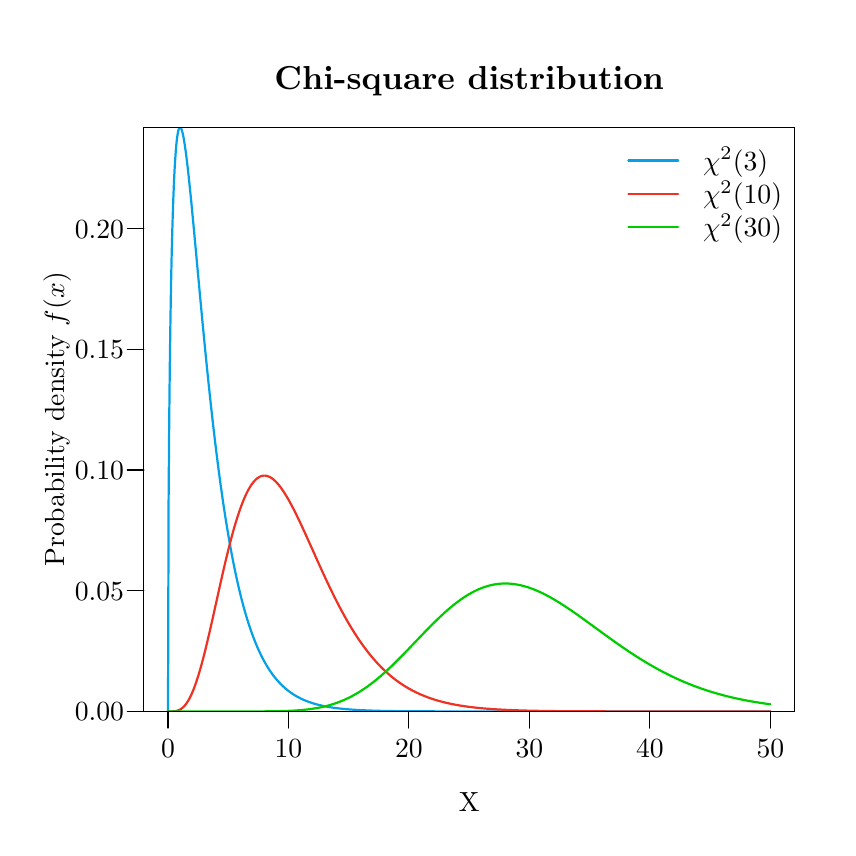
\begin{tikzpicture}[x=1pt,y=1pt]
\definecolor{fillColor}{RGB}{255,255,255}
\path[use as bounding box,fill=fillColor,fill opacity=0.00] (0,0) rectangle (289.08,289.08);
\begin{scope}
\path[clip] ( 42.00, 42.00) rectangle (277.08,253.08);
\definecolor{drawColor}{RGB}{5,161,230}

\path[draw=drawColor,line width= 0.8pt,line join=round,line cap=round] ( 50.71, 42.00) --
	( 50.92,117.90) --
	( 51.14,146.68) --
	( 51.36,167.05) --
	( 51.58,182.83) --
	( 51.79,195.56) --
	( 52.01,206.06) --
	( 52.23,214.83) --
	( 52.45,222.20) --
	( 52.67,228.42) --
	( 52.88,233.65) --
	( 53.10,238.04) --
	( 53.32,241.70) --
	( 53.54,244.72) --
	( 53.75,247.18) --
	( 53.97,249.14) --
	( 54.19,250.65) --
	( 54.41,251.76) --
	( 54.62,252.52) --
	( 54.84,252.94) --
	( 55.06,253.08) --
	( 55.28,252.95) --
	( 55.50,252.59) --
	( 55.71,252.00) --
	( 55.93,251.22) --
	( 56.15,250.26) --
	( 56.37,249.15) --
	( 56.58,247.88) --
	( 56.80,246.48) --
	( 57.02,244.96) --
	( 57.24,243.33) --
	( 57.45,241.61) --
	( 57.67,239.80) --
	( 57.89,237.90) --
	( 58.11,235.94) --
	( 58.32,233.91) --
	( 58.54,231.83) --
	( 58.76,229.70) --
	( 58.98,227.52) --
	( 59.20,225.31) --
	( 59.41,223.06) --
	( 59.63,220.78) --
	( 59.85,218.48) --
	( 60.07,216.16) --
	( 60.28,213.82) --
	( 60.50,211.47) --
	( 60.72,209.12) --
	( 60.94,206.75) --
	( 61.15,204.39) --
	( 61.37,202.02) --
	( 61.59,199.65) --
	( 61.81,197.29) --
	( 62.03,194.93) --
	( 62.24,192.58) --
	( 62.46,190.24) --
	( 62.68,187.92) --
	( 62.90,185.60) --
	( 63.11,183.30) --
	( 63.33,181.02) --
	( 63.55,178.75) --
	( 63.77,176.50) --
	( 63.98,174.27) --
	( 64.20,172.05) --
	( 64.42,169.86) --
	( 64.64,167.69) --
	( 64.85,165.54) --
	( 65.07,163.41) --
	( 65.29,161.31) --
	( 65.51,159.23) --
	( 65.73,157.17) --
	( 65.94,155.14) --
	( 66.16,153.13) --
	( 66.38,151.15) --
	( 66.60,149.19) --
	( 66.81,147.26) --
	( 67.03,145.35) --
	( 67.25,143.47) --
	( 67.47,141.61) --
	( 67.68,139.78) --
	( 67.90,137.98) --
	( 68.12,136.20) --
	( 68.34,134.44) --
	( 68.56,132.72) --
	( 68.77,131.01) --
	( 68.99,129.34) --
	( 69.21,127.69) --
	( 69.43,126.06) --
	( 69.64,124.46) --
	( 69.86,122.89) --
	( 70.08,121.34) --
	( 70.30,119.81) --
	( 70.51,118.31) --
	( 70.73,116.83) --
	( 70.95,115.38) --
	( 71.17,113.95) --
	( 71.38,112.55) --
	( 71.60,111.17) --
	( 71.82,109.81) --
	( 72.04,108.48) --
	( 72.26,107.17) --
	( 72.47,105.88) --
	( 72.69,104.61) --
	( 72.91,103.37) --
	( 73.13,102.14) --
	( 73.34,100.94) --
	( 73.56, 99.76) --
	( 73.78, 98.60) --
	( 74.00, 97.47) --
	( 74.21, 96.35) --
	( 74.43, 95.25) --
	( 74.65, 94.18) --
	( 74.87, 93.12) --
	( 75.09, 92.08) --
	( 75.30, 91.06) --
	( 75.52, 90.06) --
	( 75.74, 89.08) --
	( 75.96, 88.12) --
	( 76.17, 87.17) --
	( 76.39, 86.24) --
	( 76.61, 85.33) --
	( 76.83, 84.44) --
	( 77.04, 83.57) --
	( 77.26, 82.71) --
	( 77.48, 81.86) --
	( 77.70, 81.04) --
	( 77.91, 80.23) --
	( 78.13, 79.43) --
	( 78.35, 78.65) --
	( 78.57, 77.89) --
	( 78.79, 77.14) --
	( 79.00, 76.40) --
	( 79.22, 75.68) --
	( 79.44, 74.98) --
	( 79.66, 74.28) --
	( 79.87, 73.60) --
	( 80.09, 72.94) --
	( 80.31, 72.29) --
	( 80.53, 71.65) --
	( 80.74, 71.02) --
	( 80.96, 70.41) --
	( 81.18, 69.80) --
	( 81.40, 69.21) --
	( 81.62, 68.64) --
	( 81.83, 68.07) --
	( 82.05, 67.52) --
	( 82.27, 66.97) --
	( 82.49, 66.44) --
	( 82.70, 65.92) --
	( 82.92, 65.41) --
	( 83.14, 64.90) --
	( 83.36, 64.41) --
	( 83.57, 63.93) --
	( 83.79, 63.46) --
	( 84.01, 63.00) --
	( 84.23, 62.55) --
	( 84.44, 62.11) --
	( 84.66, 61.67) --
	( 84.88, 61.25) --
	( 85.10, 60.83) --
	( 85.32, 60.43) --
	( 85.53, 60.03) --
	( 85.75, 59.64) --
	( 85.97, 59.26) --
	( 86.19, 58.88) --
	( 86.40, 58.52) --
	( 86.62, 58.16) --
	( 86.84, 57.81) --
	( 87.06, 57.46) --
	( 87.27, 57.13) --
	( 87.49, 56.80) --
	( 87.71, 56.47) --
	( 87.93, 56.16) --
	( 88.15, 55.85) --
	( 88.36, 55.54) --
	( 88.58, 55.25) --
	( 88.80, 54.96) --
	( 89.02, 54.67) --
	( 89.23, 54.40) --
	( 89.45, 54.12) --
	( 89.67, 53.86) --
	( 89.89, 53.60) --
	( 90.10, 53.34) --
	( 90.32, 53.09) --
	( 90.54, 52.85) --
	( 90.76, 52.61) --
	( 90.97, 52.38) --
	( 91.19, 52.15) --
	( 91.41, 51.92) --
	( 91.63, 51.70) --
	( 91.85, 51.49) --
	( 92.06, 51.28) --
	( 92.28, 51.07) --
	( 92.50, 50.87) --
	( 92.72, 50.68) --
	( 92.93, 50.49) --
	( 93.15, 50.30) --
	( 93.37, 50.11) --
	( 93.59, 49.93) --
	( 93.80, 49.76) --
	( 94.02, 49.58) --
	( 94.24, 49.42) --
	( 94.46, 49.25) --
	( 94.68, 49.09) --
	( 94.89, 48.93) --
	( 95.11, 48.78) --
	( 95.33, 48.63) --
	( 95.55, 48.48) --
	( 95.76, 48.33) --
	( 95.98, 48.19) --
	( 96.20, 48.05) --
	( 96.42, 47.92) --
	( 96.63, 47.79) --
	( 96.85, 47.66) --
	( 97.07, 47.53) --
	( 97.29, 47.41) --
	( 97.50, 47.28) --
	( 97.72, 47.17) --
	( 97.94, 47.05) --
	( 98.16, 46.94) --
	( 98.38, 46.83) --
	( 98.59, 46.72) --
	( 98.81, 46.61) --
	( 99.03, 46.51) --
	( 99.25, 46.41) --
	( 99.46, 46.31) --
	( 99.68, 46.21) --
	( 99.90, 46.11) --
	(100.12, 46.02) --
	(100.33, 45.93) --
	(100.55, 45.84) --
	(100.77, 45.76) --
	(100.99, 45.67) --
	(101.21, 45.59) --
	(101.42, 45.51) --
	(101.64, 45.43) --
	(101.86, 45.35) --
	(102.08, 45.27) --
	(102.29, 45.20) --
	(102.51, 45.13) --
	(102.73, 45.06) --
	(102.95, 44.99) --
	(103.16, 44.92) --
	(103.38, 44.85) --
	(103.60, 44.79) --
	(103.82, 44.73) --
	(104.03, 44.66) --
	(104.25, 44.60) --
	(104.47, 44.54) --
	(104.69, 44.49) --
	(104.91, 44.43) --
	(105.12, 44.38) --
	(105.34, 44.32) --
	(105.56, 44.27) --
	(105.78, 44.22) --
	(105.99, 44.17) --
	(106.21, 44.12) --
	(106.43, 44.07) --
	(106.65, 44.02) --
	(106.86, 43.98) --
	(107.08, 43.93) --
	(107.30, 43.89) --
	(107.52, 43.84) --
	(107.74, 43.80) --
	(107.95, 43.76) --
	(108.17, 43.72) --
	(108.39, 43.68) --
	(108.61, 43.64) --
	(108.82, 43.60) --
	(109.04, 43.57) --
	(109.26, 43.53) --
	(109.48, 43.50) --
	(109.69, 43.46) --
	(109.91, 43.43) --
	(110.13, 43.40) --
	(110.35, 43.36) --
	(110.56, 43.33) --
	(110.78, 43.30) --
	(111.00, 43.27) --
	(111.22, 43.24) --
	(111.44, 43.22) --
	(111.65, 43.19) --
	(111.87, 43.16) --
	(112.09, 43.13) --
	(112.31, 43.11) --
	(112.52, 43.08) --
	(112.74, 43.06) --
	(112.96, 43.03) --
	(113.18, 43.01) --
	(113.39, 42.99) --
	(113.61, 42.96) --
	(113.83, 42.94) --
	(114.05, 42.92) --
	(114.27, 42.90) --
	(114.48, 42.88) --
	(114.70, 42.86) --
	(114.92, 42.84) --
	(115.14, 42.82) --
	(115.35, 42.80) --
	(115.57, 42.78) --
	(115.79, 42.76) --
	(116.01, 42.75) --
	(116.22, 42.73) --
	(116.44, 42.71) --
	(116.66, 42.70) --
	(116.88, 42.68) --
	(117.09, 42.66) --
	(117.31, 42.65) --
	(117.53, 42.63) --
	(117.75, 42.62) --
	(117.97, 42.60) --
	(118.18, 42.59) --
	(118.40, 42.58) --
	(118.62, 42.56) --
	(118.84, 42.55) --
	(119.05, 42.54) --
	(119.27, 42.53) --
	(119.49, 42.51) --
	(119.71, 42.50) --
	(119.92, 42.49) --
	(120.14, 42.48) --
	(120.36, 42.47) --
	(120.58, 42.46) --
	(120.80, 42.45) --
	(121.01, 42.44) --
	(121.23, 42.43) --
	(121.45, 42.42) --
	(121.67, 42.41) --
	(121.88, 42.40) --
	(122.10, 42.39) --
	(122.32, 42.38) --
	(122.54, 42.37) --
	(122.75, 42.36) --
	(122.97, 42.35) --
	(123.19, 42.34) --
	(123.41, 42.34) --
	(123.62, 42.33) --
	(123.84, 42.32) --
	(124.06, 42.31) --
	(124.28, 42.31) --
	(124.50, 42.30) --
	(124.71, 42.29) --
	(124.93, 42.29) --
	(125.15, 42.28) --
	(125.37, 42.27) --
	(125.58, 42.27) --
	(125.80, 42.26) --
	(126.02, 42.25) --
	(126.24, 42.25) --
	(126.45, 42.24) --
	(126.67, 42.24) --
	(126.89, 42.23) --
	(127.11, 42.23) --
	(127.33, 42.22) --
	(127.54, 42.21) --
	(127.76, 42.21) --
	(127.98, 42.21) --
	(128.20, 42.20) --
	(128.41, 42.20) --
	(128.63, 42.19) --
	(128.85, 42.19) --
	(129.07, 42.18) --
	(129.28, 42.18) --
	(129.50, 42.17) --
	(129.72, 42.17) --
	(129.94, 42.17) --
	(130.16, 42.16) --
	(130.37, 42.16) --
	(130.59, 42.15) --
	(130.81, 42.15) --
	(131.03, 42.15) --
	(131.24, 42.14) --
	(131.46, 42.14) --
	(131.68, 42.14) --
	(131.90, 42.13) --
	(132.11, 42.13) --
	(132.33, 42.13) --
	(132.55, 42.12) --
	(132.77, 42.12) --
	(132.98, 42.12) --
	(133.20, 42.12) --
	(133.42, 42.11) --
	(133.64, 42.11) --
	(133.86, 42.11) --
	(134.07, 42.11) --
	(134.29, 42.10) --
	(134.51, 42.10) --
	(134.73, 42.10) --
	(134.94, 42.10) --
	(135.16, 42.09) --
	(135.38, 42.09) --
	(135.60, 42.09) --
	(135.81, 42.09) --
	(136.03, 42.09) --
	(136.25, 42.08) --
	(136.47, 42.08) --
	(136.68, 42.08) --
	(136.90, 42.08) --
	(137.12, 42.08) --
	(137.34, 42.07) --
	(137.56, 42.07) --
	(137.77, 42.07) --
	(137.99, 42.07) --
	(138.21, 42.07) --
	(138.43, 42.07) --
	(138.64, 42.06) --
	(138.86, 42.06) --
	(139.08, 42.06) --
	(139.30, 42.06) --
	(139.51, 42.06) --
	(139.73, 42.06) --
	(139.95, 42.06) --
	(140.17, 42.05) --
	(140.39, 42.05) --
	(140.60, 42.05) --
	(140.82, 42.05) --
	(141.04, 42.05) --
	(141.26, 42.05) --
	(141.47, 42.05) --
	(141.69, 42.05) --
	(141.91, 42.04) --
	(142.13, 42.04) --
	(142.34, 42.04) --
	(142.56, 42.04) --
	(142.78, 42.04) --
	(143.00, 42.04) --
	(143.21, 42.04) --
	(143.43, 42.04) --
	(143.65, 42.04) --
	(143.87, 42.04) --
	(144.09, 42.04) --
	(144.30, 42.03) --
	(144.52, 42.03) --
	(144.74, 42.03) --
	(144.96, 42.03) --
	(145.17, 42.03) --
	(145.39, 42.03) --
	(145.61, 42.03) --
	(145.83, 42.03) --
	(146.04, 42.03) --
	(146.26, 42.03) --
	(146.48, 42.03) --
	(146.70, 42.03) --
	(146.92, 42.03) --
	(147.13, 42.03) --
	(147.35, 42.02) --
	(147.57, 42.02) --
	(147.79, 42.02) --
	(148.00, 42.02) --
	(148.22, 42.02) --
	(148.44, 42.02) --
	(148.66, 42.02) --
	(148.87, 42.02) --
	(149.09, 42.02) --
	(149.31, 42.02) --
	(149.53, 42.02) --
	(149.74, 42.02) --
	(149.96, 42.02) --
	(150.18, 42.02) --
	(150.40, 42.02) --
	(150.62, 42.02) --
	(150.83, 42.02) --
	(151.05, 42.02) --
	(151.27, 42.02) --
	(151.49, 42.02) --
	(151.70, 42.02) --
	(151.92, 42.02) --
	(152.14, 42.01) --
	(152.36, 42.01) --
	(152.57, 42.01) --
	(152.79, 42.01) --
	(153.01, 42.01) --
	(153.23, 42.01) --
	(153.45, 42.01) --
	(153.66, 42.01) --
	(153.88, 42.01) --
	(154.10, 42.01) --
	(154.32, 42.01) --
	(154.53, 42.01) --
	(154.75, 42.01) --
	(154.97, 42.01) --
	(155.19, 42.01) --
	(155.40, 42.01) --
	(155.62, 42.01) --
	(155.84, 42.01) --
	(156.06, 42.01) --
	(156.27, 42.01) --
	(156.49, 42.01) --
	(156.71, 42.01) --
	(156.93, 42.01) --
	(157.15, 42.01) --
	(157.36, 42.01) --
	(157.58, 42.01) --
	(157.80, 42.01) --
	(158.02, 42.01) --
	(158.23, 42.01) --
	(158.45, 42.01) --
	(158.67, 42.01) --
	(158.89, 42.01) --
	(159.10, 42.01) --
	(159.32, 42.01) --
	(159.54, 42.01) --
	(159.76, 42.01) --
	(159.98, 42.01) --
	(160.19, 42.01) --
	(160.41, 42.01) --
	(160.63, 42.01) --
	(160.85, 42.01) --
	(161.06, 42.01) --
	(161.28, 42.01) --
	(161.50, 42.01) --
	(161.72, 42.01) --
	(161.93, 42.00) --
	(162.15, 42.00) --
	(162.37, 42.00) --
	(162.59, 42.00) --
	(162.80, 42.00) --
	(163.02, 42.00) --
	(163.24, 42.00) --
	(163.46, 42.00) --
	(163.68, 42.00) --
	(163.89, 42.00) --
	(164.11, 42.00) --
	(164.33, 42.00) --
	(164.55, 42.00) --
	(164.76, 42.00) --
	(164.98, 42.00) --
	(165.20, 42.00) --
	(165.42, 42.00) --
	(165.63, 42.00) --
	(165.85, 42.00) --
	(166.07, 42.00) --
	(166.29, 42.00) --
	(166.51, 42.00) --
	(166.72, 42.00) --
	(166.94, 42.00) --
	(167.16, 42.00) --
	(167.38, 42.00) --
	(167.59, 42.00) --
	(167.81, 42.00) --
	(168.03, 42.00) --
	(168.25, 42.00) --
	(168.46, 42.00) --
	(168.68, 42.00) --
	(168.90, 42.00) --
	(169.12, 42.00) --
	(169.33, 42.00) --
	(169.55, 42.00) --
	(169.77, 42.00) --
	(169.99, 42.00) --
	(170.21, 42.00) --
	(170.42, 42.00) --
	(170.64, 42.00) --
	(170.86, 42.00) --
	(171.08, 42.00) --
	(171.29, 42.00) --
	(171.51, 42.00) --
	(171.73, 42.00) --
	(171.95, 42.00) --
	(172.16, 42.00) --
	(172.38, 42.00) --
	(172.60, 42.00) --
	(172.82, 42.00) --
	(173.04, 42.00) --
	(173.25, 42.00) --
	(173.47, 42.00) --
	(173.69, 42.00) --
	(173.91, 42.00) --
	(174.12, 42.00) --
	(174.34, 42.00) --
	(174.56, 42.00) --
	(174.78, 42.00) --
	(174.99, 42.00) --
	(175.21, 42.00) --
	(175.43, 42.00) --
	(175.65, 42.00) --
	(175.86, 42.00) --
	(176.08, 42.00) --
	(176.30, 42.00) --
	(176.52, 42.00) --
	(176.74, 42.00) --
	(176.95, 42.00) --
	(177.17, 42.00) --
	(177.39, 42.00) --
	(177.61, 42.00) --
	(177.82, 42.00) --
	(178.04, 42.00) --
	(178.26, 42.00) --
	(178.48, 42.00) --
	(178.69, 42.00) --
	(178.91, 42.00) --
	(179.13, 42.00) --
	(179.35, 42.00) --
	(179.57, 42.00) --
	(179.78, 42.00) --
	(180.00, 42.00) --
	(180.22, 42.00) --
	(180.44, 42.00) --
	(180.65, 42.00) --
	(180.87, 42.00) --
	(181.09, 42.00) --
	(181.31, 42.00) --
	(181.52, 42.00) --
	(181.74, 42.00) --
	(181.96, 42.00) --
	(182.18, 42.00) --
	(182.39, 42.00) --
	(182.61, 42.00) --
	(182.83, 42.00) --
	(183.05, 42.00) --
	(183.27, 42.00) --
	(183.48, 42.00) --
	(183.70, 42.00) --
	(183.92, 42.00) --
	(184.14, 42.00) --
	(184.35, 42.00) --
	(184.57, 42.00) --
	(184.79, 42.00) --
	(185.01, 42.00) --
	(185.22, 42.00) --
	(185.44, 42.00) --
	(185.66, 42.00) --
	(185.88, 42.00) --
	(186.10, 42.00) --
	(186.31, 42.00) --
	(186.53, 42.00) --
	(186.75, 42.00) --
	(186.97, 42.00) --
	(187.18, 42.00) --
	(187.40, 42.00) --
	(187.62, 42.00) --
	(187.84, 42.00) --
	(188.05, 42.00) --
	(188.27, 42.00) --
	(188.49, 42.00) --
	(188.71, 42.00) --
	(188.92, 42.00) --
	(189.14, 42.00) --
	(189.36, 42.00) --
	(189.58, 42.00) --
	(189.80, 42.00) --
	(190.01, 42.00) --
	(190.23, 42.00) --
	(190.45, 42.00) --
	(190.67, 42.00) --
	(190.88, 42.00) --
	(191.10, 42.00) --
	(191.32, 42.00) --
	(191.54, 42.00) --
	(191.75, 42.00) --
	(191.97, 42.00) --
	(192.19, 42.00) --
	(192.41, 42.00) --
	(192.63, 42.00) --
	(192.84, 42.00) --
	(193.06, 42.00) --
	(193.28, 42.00) --
	(193.50, 42.00) --
	(193.71, 42.00) --
	(193.93, 42.00) --
	(194.15, 42.00) --
	(194.37, 42.00) --
	(194.58, 42.00) --
	(194.80, 42.00) --
	(195.02, 42.00) --
	(195.24, 42.00) --
	(195.45, 42.00) --
	(195.67, 42.00) --
	(195.89, 42.00) --
	(196.11, 42.00) --
	(196.33, 42.00) --
	(196.54, 42.00) --
	(196.76, 42.00) --
	(196.98, 42.00) --
	(197.20, 42.00) --
	(197.41, 42.00) --
	(197.63, 42.00) --
	(197.85, 42.00) --
	(198.07, 42.00) --
	(198.28, 42.00) --
	(198.50, 42.00) --
	(198.72, 42.00) --
	(198.94, 42.00) --
	(199.16, 42.00) --
	(199.37, 42.00) --
	(199.59, 42.00) --
	(199.81, 42.00) --
	(200.03, 42.00) --
	(200.24, 42.00) --
	(200.46, 42.00) --
	(200.68, 42.00) --
	(200.90, 42.00) --
	(201.11, 42.00) --
	(201.33, 42.00) --
	(201.55, 42.00) --
	(201.77, 42.00) --
	(201.98, 42.00) --
	(202.20, 42.00) --
	(202.42, 42.00) --
	(202.64, 42.00) --
	(202.86, 42.00) --
	(203.07, 42.00) --
	(203.29, 42.00) --
	(203.51, 42.00) --
	(203.73, 42.00) --
	(203.94, 42.00) --
	(204.16, 42.00) --
	(204.38, 42.00) --
	(204.60, 42.00) --
	(204.81, 42.00) --
	(205.03, 42.00) --
	(205.25, 42.00) --
	(205.47, 42.00) --
	(205.69, 42.00) --
	(205.90, 42.00) --
	(206.12, 42.00) --
	(206.34, 42.00) --
	(206.56, 42.00) --
	(206.77, 42.00) --
	(206.99, 42.00) --
	(207.21, 42.00) --
	(207.43, 42.00) --
	(207.64, 42.00) --
	(207.86, 42.00) --
	(208.08, 42.00) --
	(208.30, 42.00) --
	(208.51, 42.00) --
	(208.73, 42.00) --
	(208.95, 42.00) --
	(209.17, 42.00) --
	(209.39, 42.00) --
	(209.60, 42.00) --
	(209.82, 42.00) --
	(210.04, 42.00) --
	(210.26, 42.00) --
	(210.47, 42.00) --
	(210.69, 42.00) --
	(210.91, 42.00) --
	(211.13, 42.00) --
	(211.34, 42.00) --
	(211.56, 42.00) --
	(211.78, 42.00) --
	(212.00, 42.00) --
	(212.22, 42.00) --
	(212.43, 42.00) --
	(212.65, 42.00) --
	(212.87, 42.00) --
	(213.09, 42.00) --
	(213.30, 42.00) --
	(213.52, 42.00) --
	(213.74, 42.00) --
	(213.96, 42.00) --
	(214.17, 42.00) --
	(214.39, 42.00) --
	(214.61, 42.00) --
	(214.83, 42.00) --
	(215.04, 42.00) --
	(215.26, 42.00) --
	(215.48, 42.00) --
	(215.70, 42.00) --
	(215.92, 42.00) --
	(216.13, 42.00) --
	(216.35, 42.00) --
	(216.57, 42.00) --
	(216.79, 42.00) --
	(217.00, 42.00) --
	(217.22, 42.00) --
	(217.44, 42.00) --
	(217.66, 42.00) --
	(217.87, 42.00) --
	(218.09, 42.00) --
	(218.31, 42.00) --
	(218.53, 42.00) --
	(218.75, 42.00) --
	(218.96, 42.00) --
	(219.18, 42.00) --
	(219.40, 42.00) --
	(219.62, 42.00) --
	(219.83, 42.00) --
	(220.05, 42.00) --
	(220.27, 42.00) --
	(220.49, 42.00) --
	(220.70, 42.00) --
	(220.92, 42.00) --
	(221.14, 42.00) --
	(221.36, 42.00) --
	(221.57, 42.00) --
	(221.79, 42.00) --
	(222.01, 42.00) --
	(222.23, 42.00) --
	(222.45, 42.00) --
	(222.66, 42.00) --
	(222.88, 42.00) --
	(223.10, 42.00) --
	(223.32, 42.00) --
	(223.53, 42.00) --
	(223.75, 42.00) --
	(223.97, 42.00) --
	(224.19, 42.00) --
	(224.40, 42.00) --
	(224.62, 42.00) --
	(224.84, 42.00) --
	(225.06, 42.00) --
	(225.28, 42.00) --
	(225.49, 42.00) --
	(225.71, 42.00) --
	(225.93, 42.00) --
	(226.15, 42.00) --
	(226.36, 42.00) --
	(226.58, 42.00) --
	(226.80, 42.00) --
	(227.02, 42.00) --
	(227.23, 42.00) --
	(227.45, 42.00) --
	(227.67, 42.00) --
	(227.89, 42.00) --
	(228.10, 42.00) --
	(228.32, 42.00) --
	(228.54, 42.00) --
	(228.76, 42.00) --
	(228.98, 42.00) --
	(229.19, 42.00) --
	(229.41, 42.00) --
	(229.63, 42.00) --
	(229.85, 42.00) --
	(230.06, 42.00) --
	(230.28, 42.00) --
	(230.50, 42.00) --
	(230.72, 42.00) --
	(230.93, 42.00) --
	(231.15, 42.00) --
	(231.37, 42.00) --
	(231.59, 42.00) --
	(231.81, 42.00) --
	(232.02, 42.00) --
	(232.24, 42.00) --
	(232.46, 42.00) --
	(232.68, 42.00) --
	(232.89, 42.00) --
	(233.11, 42.00) --
	(233.33, 42.00) --
	(233.55, 42.00) --
	(233.76, 42.00) --
	(233.98, 42.00) --
	(234.20, 42.00) --
	(234.42, 42.00) --
	(234.63, 42.00) --
	(234.85, 42.00) --
	(235.07, 42.00) --
	(235.29, 42.00) --
	(235.51, 42.00) --
	(235.72, 42.00) --
	(235.94, 42.00) --
	(236.16, 42.00) --
	(236.38, 42.00) --
	(236.59, 42.00) --
	(236.81, 42.00) --
	(237.03, 42.00) --
	(237.25, 42.00) --
	(237.46, 42.00) --
	(237.68, 42.00) --
	(237.90, 42.00) --
	(238.12, 42.00) --
	(238.34, 42.00) --
	(238.55, 42.00) --
	(238.77, 42.00) --
	(238.99, 42.00) --
	(239.21, 42.00) --
	(239.42, 42.00) --
	(239.64, 42.00) --
	(239.86, 42.00) --
	(240.08, 42.00) --
	(240.29, 42.00) --
	(240.51, 42.00) --
	(240.73, 42.00) --
	(240.95, 42.00) --
	(241.16, 42.00) --
	(241.38, 42.00) --
	(241.60, 42.00) --
	(241.82, 42.00) --
	(242.04, 42.00) --
	(242.25, 42.00) --
	(242.47, 42.00) --
	(242.69, 42.00) --
	(242.91, 42.00) --
	(243.12, 42.00) --
	(243.34, 42.00) --
	(243.56, 42.00) --
	(243.78, 42.00) --
	(243.99, 42.00) --
	(244.21, 42.00) --
	(244.43, 42.00) --
	(244.65, 42.00) --
	(244.87, 42.00) --
	(245.08, 42.00) --
	(245.30, 42.00) --
	(245.52, 42.00) --
	(245.74, 42.00) --
	(245.95, 42.00) --
	(246.17, 42.00) --
	(246.39, 42.00) --
	(246.61, 42.00) --
	(246.82, 42.00) --
	(247.04, 42.00) --
	(247.26, 42.00) --
	(247.48, 42.00) --
	(247.69, 42.00) --
	(247.91, 42.00) --
	(248.13, 42.00) --
	(248.35, 42.00) --
	(248.57, 42.00) --
	(248.78, 42.00) --
	(249.00, 42.00) --
	(249.22, 42.00) --
	(249.44, 42.00) --
	(249.65, 42.00) --
	(249.87, 42.00) --
	(250.09, 42.00) --
	(250.31, 42.00) --
	(250.52, 42.00) --
	(250.74, 42.00) --
	(250.96, 42.00) --
	(251.18, 42.00) --
	(251.40, 42.00) --
	(251.61, 42.00) --
	(251.83, 42.00) --
	(252.05, 42.00) --
	(252.27, 42.00) --
	(252.48, 42.00) --
	(252.70, 42.00) --
	(252.92, 42.00) --
	(253.14, 42.00) --
	(253.35, 42.00) --
	(253.57, 42.00) --
	(253.79, 42.00) --
	(254.01, 42.00) --
	(254.22, 42.00) --
	(254.44, 42.00) --
	(254.66, 42.00) --
	(254.88, 42.00) --
	(255.10, 42.00) --
	(255.31, 42.00) --
	(255.53, 42.00) --
	(255.75, 42.00) --
	(255.97, 42.00) --
	(256.18, 42.00) --
	(256.40, 42.00) --
	(256.62, 42.00) --
	(256.84, 42.00) --
	(257.05, 42.00) --
	(257.27, 42.00) --
	(257.49, 42.00) --
	(257.71, 42.00) --
	(257.93, 42.00) --
	(258.14, 42.00) --
	(258.36, 42.00) --
	(258.58, 42.00) --
	(258.80, 42.00) --
	(259.01, 42.00) --
	(259.23, 42.00) --
	(259.45, 42.00) --
	(259.67, 42.00) --
	(259.88, 42.00) --
	(260.10, 42.00) --
	(260.32, 42.00) --
	(260.54, 42.00) --
	(260.75, 42.00) --
	(260.97, 42.00) --
	(261.19, 42.00) --
	(261.41, 42.00) --
	(261.63, 42.00) --
	(261.84, 42.00) --
	(262.06, 42.00) --
	(262.28, 42.00) --
	(262.50, 42.00) --
	(262.71, 42.00) --
	(262.93, 42.00) --
	(263.15, 42.00) --
	(263.37, 42.00) --
	(263.58, 42.00) --
	(263.80, 42.00) --
	(264.02, 42.00) --
	(264.24, 42.00) --
	(264.46, 42.00) --
	(264.67, 42.00) --
	(264.89, 42.00) --
	(265.11, 42.00) --
	(265.33, 42.00) --
	(265.54, 42.00) --
	(265.76, 42.00) --
	(265.98, 42.00) --
	(266.20, 42.00) --
	(266.41, 42.00) --
	(266.63, 42.00) --
	(266.85, 42.00) --
	(267.07, 42.00) --
	(267.28, 42.00) --
	(267.50, 42.00) --
	(267.72, 42.00) --
	(267.94, 42.00) --
	(268.16, 42.00) --
	(268.37, 42.00);
\end{scope}
\begin{scope}
\path[clip] (  0.00,  0.00) rectangle (289.08,289.08);
\definecolor{drawColor}{RGB}{0,0,0}

\path[draw=drawColor,line width= 0.4pt,line join=round,line cap=round] ( 50.71, 42.00) -- (268.37, 42.00);

\path[draw=drawColor,line width= 0.4pt,line join=round,line cap=round] ( 50.71, 42.00) -- ( 50.71, 36.00);

\path[draw=drawColor,line width= 0.4pt,line join=round,line cap=round] ( 94.24, 42.00) -- ( 94.24, 36.00);

\path[draw=drawColor,line width= 0.4pt,line join=round,line cap=round] (137.77, 42.00) -- (137.77, 36.00);

\path[draw=drawColor,line width= 0.4pt,line join=round,line cap=round] (181.31, 42.00) -- (181.31, 36.00);

\path[draw=drawColor,line width= 0.4pt,line join=round,line cap=round] (224.84, 42.00) -- (224.84, 36.00);

\path[draw=drawColor,line width= 0.4pt,line join=round,line cap=round] (268.37, 42.00) -- (268.37, 36.00);

\node[text=drawColor,anchor=base,inner sep=0pt, outer sep=0pt, scale=  1.00] at ( 50.71, 25.20) {0};

\node[text=drawColor,anchor=base,inner sep=0pt, outer sep=0pt, scale=  1.00] at ( 94.24, 25.20) {10};

\node[text=drawColor,anchor=base,inner sep=0pt, outer sep=0pt, scale=  1.00] at (137.77, 25.20) {20};

\node[text=drawColor,anchor=base,inner sep=0pt, outer sep=0pt, scale=  1.00] at (181.31, 25.20) {30};

\node[text=drawColor,anchor=base,inner sep=0pt, outer sep=0pt, scale=  1.00] at (224.84, 25.20) {40};

\node[text=drawColor,anchor=base,inner sep=0pt, outer sep=0pt, scale=  1.00] at (268.37, 25.20) {50};

\path[draw=drawColor,line width= 0.4pt,line join=round,line cap=round] ( 42.00, 42.00) -- ( 42.00,216.47);

\path[draw=drawColor,line width= 0.4pt,line join=round,line cap=round] ( 42.00, 42.00) -- ( 36.00, 42.00);

\path[draw=drawColor,line width= 0.4pt,line join=round,line cap=round] ( 42.00, 85.62) -- ( 36.00, 85.62);

\path[draw=drawColor,line width= 0.4pt,line join=round,line cap=round] ( 42.00,129.23) -- ( 36.00,129.23);

\path[draw=drawColor,line width= 0.4pt,line join=round,line cap=round] ( 42.00,172.85) -- ( 36.00,172.85);

\path[draw=drawColor,line width= 0.4pt,line join=round,line cap=round] ( 42.00,216.47) -- ( 36.00,216.47);

\node[text=drawColor,anchor=base east,inner sep=0pt, outer sep=0pt, scale=  1.00] at ( 34.80, 38.56) {0.00};

\node[text=drawColor,anchor=base east,inner sep=0pt, outer sep=0pt, scale=  1.00] at ( 34.80, 82.17) {0.05};

\node[text=drawColor,anchor=base east,inner sep=0pt, outer sep=0pt, scale=  1.00] at ( 34.80,125.79) {0.10};

\node[text=drawColor,anchor=base east,inner sep=0pt, outer sep=0pt, scale=  1.00] at ( 34.80,169.41) {0.15};

\node[text=drawColor,anchor=base east,inner sep=0pt, outer sep=0pt, scale=  1.00] at ( 34.80,213.02) {0.20};

\path[draw=drawColor,line width= 0.4pt,line join=round,line cap=round] ( 42.00, 42.00) --
	(277.08, 42.00) --
	(277.08,253.08) --
	( 42.00,253.08) --
	( 42.00, 42.00);
\end{scope}
\begin{scope}
\path[clip] (  0.00,  0.00) rectangle (289.08,289.08);
\definecolor{drawColor}{RGB}{0,0,0}

\node[text=drawColor,anchor=base,inner sep=0pt, outer sep=0pt, scale=  1.20] at (159.54,266.89) {\bfseries Chi-square distribution};

\node[text=drawColor,anchor=base,inner sep=0pt, outer sep=0pt, scale=  1.00] at (159.54,  6.00) {X};

\node[text=drawColor,rotate= 90.00,anchor=base,inner sep=0pt, outer sep=0pt, scale=  1.00] at ( 13.20,147.54) {Probability density $f(x)$};
\end{scope}
\begin{scope}
\path[clip] ( 42.00, 42.00) rectangle (277.08,253.08);
\definecolor{drawColor}{RGB}{238,50,36}

\path[draw=drawColor,line width= 0.8pt,line join=round,line cap=round] ( 50.71, 42.00) --
	( 50.92, 42.00) --
	( 51.14, 42.00) --
	( 51.36, 42.00) --
	( 51.58, 42.00) --
	( 51.79, 42.00) --
	( 52.01, 42.01) --
	( 52.23, 42.01) --
	( 52.45, 42.02) --
	( 52.67, 42.04) --
	( 52.88, 42.06) --
	( 53.10, 42.08) --
	( 53.32, 42.11) --
	( 53.54, 42.15) --
	( 53.75, 42.19) --
	( 53.97, 42.25) --
	( 54.19, 42.31) --
	( 54.41, 42.39) --
	( 54.62, 42.48) --
	( 54.84, 42.58) --
	( 55.06, 42.69) --
	( 55.28, 42.82) --
	( 55.50, 42.96) --
	( 55.71, 43.12) --
	( 55.93, 43.29) --
	( 56.15, 43.48) --
	( 56.37, 43.69) --
	( 56.58, 43.92) --
	( 56.80, 44.17) --
	( 57.02, 44.43) --
	( 57.24, 44.72) --
	( 57.45, 45.02) --
	( 57.67, 45.34) --
	( 57.89, 45.69) --
	( 58.11, 46.05) --
	( 58.32, 46.44) --
	( 58.54, 46.85) --
	( 58.76, 47.28) --
	( 58.98, 47.72) --
	( 59.20, 48.19) --
	( 59.41, 48.69) --
	( 59.63, 49.20) --
	( 59.85, 49.73) --
	( 60.07, 50.28) --
	( 60.28, 50.86) --
	( 60.50, 51.45) --
	( 60.72, 52.06) --
	( 60.94, 52.70) --
	( 61.15, 53.35) --
	( 61.37, 54.02) --
	( 61.59, 54.71) --
	( 61.81, 55.42) --
	( 62.03, 56.15) --
	( 62.24, 56.89) --
	( 62.46, 57.65) --
	( 62.68, 58.42) --
	( 62.90, 59.22) --
	( 63.11, 60.02) --
	( 63.33, 60.84) --
	( 63.55, 61.68) --
	( 63.77, 62.53) --
	( 63.98, 63.39) --
	( 64.20, 64.26) --
	( 64.42, 65.15) --
	( 64.64, 66.05) --
	( 64.85, 66.95) --
	( 65.07, 67.87) --
	( 65.29, 68.80) --
	( 65.51, 69.73) --
	( 65.73, 70.67) --
	( 65.94, 71.62) --
	( 66.16, 72.57) --
	( 66.38, 73.54) --
	( 66.60, 74.50) --
	( 66.81, 75.47) --
	( 67.03, 76.45) --
	( 67.25, 77.42) --
	( 67.47, 78.40) --
	( 67.68, 79.39) --
	( 67.90, 80.37) --
	( 68.12, 81.35) --
	( 68.34, 82.34) --
	( 68.56, 83.32) --
	( 68.77, 84.30) --
	( 68.99, 85.28) --
	( 69.21, 86.26) --
	( 69.43, 87.23) --
	( 69.64, 88.21) --
	( 69.86, 89.17) --
	( 70.08, 90.13) --
	( 70.30, 91.09) --
	( 70.51, 92.04) --
	( 70.73, 92.99) --
	( 70.95, 93.93) --
	( 71.17, 94.86) --
	( 71.38, 95.78) --
	( 71.60, 96.70) --
	( 71.82, 97.61) --
	( 72.04, 98.50) --
	( 72.26, 99.39) --
	( 72.47,100.27) --
	( 72.69,101.14) --
	( 72.91,102.00) --
	( 73.13,102.85) --
	( 73.34,103.68) --
	( 73.56,104.51) --
	( 73.78,105.32) --
	( 74.00,106.12) --
	( 74.21,106.91) --
	( 74.43,107.68) --
	( 74.65,108.45) --
	( 74.87,109.19) --
	( 75.09,109.93) --
	( 75.30,110.65) --
	( 75.52,111.36) --
	( 75.74,112.05) --
	( 75.96,112.73) --
	( 76.17,113.39) --
	( 76.39,114.04) --
	( 76.61,114.67) --
	( 76.83,115.29) --
	( 77.04,115.89) --
	( 77.26,116.48) --
	( 77.48,117.05) --
	( 77.70,117.61) --
	( 77.91,118.15) --
	( 78.13,118.68) --
	( 78.35,119.19) --
	( 78.57,119.68) --
	( 78.79,120.16) --
	( 79.00,120.62) --
	( 79.22,121.06) --
	( 79.44,121.49) --
	( 79.66,121.91) --
	( 79.87,122.30) --
	( 80.09,122.69) --
	( 80.31,123.05) --
	( 80.53,123.40) --
	( 80.74,123.73) --
	( 80.96,124.05) --
	( 81.18,124.35) --
	( 81.40,124.64) --
	( 81.62,124.91) --
	( 81.83,125.17) --
	( 82.05,125.41) --
	( 82.27,125.63) --
	( 82.49,125.84) --
	( 82.70,126.03) --
	( 82.92,126.21) --
	( 83.14,126.37) --
	( 83.36,126.52) --
	( 83.57,126.65) --
	( 83.79,126.77) --
	( 84.01,126.88) --
	( 84.23,126.97) --
	( 84.44,127.04) --
	( 84.66,127.10) --
	( 84.88,127.15) --
	( 85.10,127.19) --
	( 85.32,127.21) --
	( 85.53,127.21) --
	( 85.75,127.21) --
	( 85.97,127.19) --
	( 86.19,127.15) --
	( 86.40,127.11) --
	( 86.62,127.05) --
	( 86.84,126.98) --
	( 87.06,126.90) --
	( 87.27,126.80) --
	( 87.49,126.69) --
	( 87.71,126.58) --
	( 87.93,126.45) --
	( 88.15,126.30) --
	( 88.36,126.15) --
	( 88.58,125.99) --
	( 88.80,125.81) --
	( 89.02,125.63) --
	( 89.23,125.43) --
	( 89.45,125.23) --
	( 89.67,125.01) --
	( 89.89,124.79) --
	( 90.10,124.55) --
	( 90.32,124.31) --
	( 90.54,124.06) --
	( 90.76,123.79) --
	( 90.97,123.52) --
	( 91.19,123.24) --
	( 91.41,122.95) --
	( 91.63,122.66) --
	( 91.85,122.35) --
	( 92.06,122.04) --
	( 92.28,121.72) --
	( 92.50,121.40) --
	( 92.72,121.06) --
	( 92.93,120.72) --
	( 93.15,120.37) --
	( 93.37,120.02) --
	( 93.59,119.65) --
	( 93.80,119.29) --
	( 94.02,118.91) --
	( 94.24,118.53) --
	( 94.46,118.15) --
	( 94.68,117.76) --
	( 94.89,117.36) --
	( 95.11,116.96) --
	( 95.33,116.55) --
	( 95.55,116.14) --
	( 95.76,115.72) --
	( 95.98,115.30) --
	( 96.20,114.88) --
	( 96.42,114.45) --
	( 96.63,114.02) --
	( 96.85,113.58) --
	( 97.07,113.14) --
	( 97.29,112.69) --
	( 97.50,112.25) --
	( 97.72,111.80) --
	( 97.94,111.34) --
	( 98.16,110.88) --
	( 98.38,110.43) --
	( 98.59,109.96) --
	( 98.81,109.50) --
	( 99.03,109.03) --
	( 99.25,108.56) --
	( 99.46,108.09) --
	( 99.68,107.62) --
	( 99.90,107.14) --
	(100.12,106.67) --
	(100.33,106.19) --
	(100.55,105.71) --
	(100.77,105.23) --
	(100.99,104.75) --
	(101.21,104.27) --
	(101.42,103.78) --
	(101.64,103.30) --
	(101.86,102.81) --
	(102.08,102.33) --
	(102.29,101.84) --
	(102.51,101.36) --
	(102.73,100.87) --
	(102.95,100.38) --
	(103.16, 99.90) --
	(103.38, 99.41) --
	(103.60, 98.92) --
	(103.82, 98.44) --
	(104.03, 97.95) --
	(104.25, 97.47) --
	(104.47, 96.98) --
	(104.69, 96.50) --
	(104.91, 96.02) --
	(105.12, 95.53) --
	(105.34, 95.05) --
	(105.56, 94.57) --
	(105.78, 94.09) --
	(105.99, 93.61) --
	(106.21, 93.14) --
	(106.43, 92.66) --
	(106.65, 92.19) --
	(106.86, 91.71) --
	(107.08, 91.24) --
	(107.30, 90.77) --
	(107.52, 90.31) --
	(107.74, 89.84) --
	(107.95, 89.37) --
	(108.17, 88.91) --
	(108.39, 88.45) --
	(108.61, 87.99) --
	(108.82, 87.53) --
	(109.04, 87.08) --
	(109.26, 86.63) --
	(109.48, 86.17) --
	(109.69, 85.73) --
	(109.91, 85.28) --
	(110.13, 84.83) --
	(110.35, 84.39) --
	(110.56, 83.95) --
	(110.78, 83.52) --
	(111.00, 83.08) --
	(111.22, 82.65) --
	(111.44, 82.22) --
	(111.65, 81.79) --
	(111.87, 81.36) --
	(112.09, 80.94) --
	(112.31, 80.52) --
	(112.52, 80.11) --
	(112.74, 79.69) --
	(112.96, 79.28) --
	(113.18, 78.87) --
	(113.39, 78.46) --
	(113.61, 78.06) --
	(113.83, 77.66) --
	(114.05, 77.26) --
	(114.27, 76.86) --
	(114.48, 76.47) --
	(114.70, 76.08) --
	(114.92, 75.70) --
	(115.14, 75.31) --
	(115.35, 74.93) --
	(115.57, 74.55) --
	(115.79, 74.18) --
	(116.01, 73.80) --
	(116.22, 73.43) --
	(116.44, 73.07) --
	(116.66, 72.70) --
	(116.88, 72.34) --
	(117.09, 71.99) --
	(117.31, 71.63) --
	(117.53, 71.28) --
	(117.75, 70.93) --
	(117.97, 70.58) --
	(118.18, 70.24) --
	(118.40, 69.90) --
	(118.62, 69.56) --
	(118.84, 69.23) --
	(119.05, 68.90) --
	(119.27, 68.57) --
	(119.49, 68.24) --
	(119.71, 67.92) --
	(119.92, 67.60) --
	(120.14, 67.29) --
	(120.36, 66.97) --
	(120.58, 66.66) --
	(120.80, 66.35) --
	(121.01, 66.05) --
	(121.23, 65.75) --
	(121.45, 65.45) --
	(121.67, 65.15) --
	(121.88, 64.86) --
	(122.10, 64.57) --
	(122.32, 64.28) --
	(122.54, 64.00) --
	(122.75, 63.71) --
	(122.97, 63.43) --
	(123.19, 63.16) --
	(123.41, 62.88) --
	(123.62, 62.61) --
	(123.84, 62.35) --
	(124.06, 62.08) --
	(124.28, 61.82) --
	(124.50, 61.56) --
	(124.71, 61.30) --
	(124.93, 61.05) --
	(125.15, 60.80) --
	(125.37, 60.55) --
	(125.58, 60.30) --
	(125.80, 60.06) --
	(126.02, 59.82) --
	(126.24, 59.58) --
	(126.45, 59.34) --
	(126.67, 59.11) --
	(126.89, 58.88) --
	(127.11, 58.65) --
	(127.33, 58.43) --
	(127.54, 58.21) --
	(127.76, 57.98) --
	(127.98, 57.77) --
	(128.20, 57.55) --
	(128.41, 57.34) --
	(128.63, 57.13) --
	(128.85, 56.92) --
	(129.07, 56.72) --
	(129.28, 56.51) --
	(129.50, 56.31) --
	(129.72, 56.11) --
	(129.94, 55.92) --
	(130.16, 55.72) --
	(130.37, 55.53) --
	(130.59, 55.34) --
	(130.81, 55.15) --
	(131.03, 54.97) --
	(131.24, 54.79) --
	(131.46, 54.61) --
	(131.68, 54.43) --
	(131.90, 54.25) --
	(132.11, 54.08) --
	(132.33, 53.91) --
	(132.55, 53.74) --
	(132.77, 53.57) --
	(132.98, 53.40) --
	(133.20, 53.24) --
	(133.42, 53.08) --
	(133.64, 52.92) --
	(133.86, 52.76) --
	(134.07, 52.61) --
	(134.29, 52.45) --
	(134.51, 52.30) --
	(134.73, 52.15) --
	(134.94, 52.01) --
	(135.16, 51.86) --
	(135.38, 51.72) --
	(135.60, 51.57) --
	(135.81, 51.43) --
	(136.03, 51.30) --
	(136.25, 51.16) --
	(136.47, 51.02) --
	(136.68, 50.89) --
	(136.90, 50.76) --
	(137.12, 50.63) --
	(137.34, 50.50) --
	(137.56, 50.38) --
	(137.77, 50.25) --
	(137.99, 50.13) --
	(138.21, 50.01) --
	(138.43, 49.89) --
	(138.64, 49.77) --
	(138.86, 49.65) --
	(139.08, 49.54) --
	(139.30, 49.42) --
	(139.51, 49.31) --
	(139.73, 49.20) --
	(139.95, 49.09) --
	(140.17, 48.99) --
	(140.39, 48.88) --
	(140.60, 48.78) --
	(140.82, 48.67) --
	(141.04, 48.57) --
	(141.26, 48.47) --
	(141.47, 48.37) --
	(141.69, 48.27) --
	(141.91, 48.18) --
	(142.13, 48.08) --
	(142.34, 47.99) --
	(142.56, 47.90) --
	(142.78, 47.81) --
	(143.00, 47.72) --
	(143.21, 47.63) --
	(143.43, 47.54) --
	(143.65, 47.46) --
	(143.87, 47.37) --
	(144.09, 47.29) --
	(144.30, 47.20) --
	(144.52, 47.12) --
	(144.74, 47.04) --
	(144.96, 46.96) --
	(145.17, 46.89) --
	(145.39, 46.81) --
	(145.61, 46.74) --
	(145.83, 46.66) --
	(146.04, 46.59) --
	(146.26, 46.52) --
	(146.48, 46.44) --
	(146.70, 46.37) --
	(146.92, 46.30) --
	(147.13, 46.24) --
	(147.35, 46.17) --
	(147.57, 46.10) --
	(147.79, 46.04) --
	(148.00, 45.97) --
	(148.22, 45.91) --
	(148.44, 45.85) --
	(148.66, 45.79) --
	(148.87, 45.73) --
	(149.09, 45.67) --
	(149.31, 45.61) --
	(149.53, 45.55) --
	(149.74, 45.49) --
	(149.96, 45.44) --
	(150.18, 45.38) --
	(150.40, 45.33) --
	(150.62, 45.27) --
	(150.83, 45.22) --
	(151.05, 45.17) --
	(151.27, 45.12) --
	(151.49, 45.07) --
	(151.70, 45.02) --
	(151.92, 44.97) --
	(152.14, 44.92) --
	(152.36, 44.87) --
	(152.57, 44.82) --
	(152.79, 44.78) --
	(153.01, 44.73) --
	(153.23, 44.69) --
	(153.45, 44.64) --
	(153.66, 44.60) --
	(153.88, 44.56) --
	(154.10, 44.52) --
	(154.32, 44.47) --
	(154.53, 44.43) --
	(154.75, 44.39) --
	(154.97, 44.35) --
	(155.19, 44.32) --
	(155.40, 44.28) --
	(155.62, 44.24) --
	(155.84, 44.20) --
	(156.06, 44.17) --
	(156.27, 44.13) --
	(156.49, 44.09) --
	(156.71, 44.06) --
	(156.93, 44.03) --
	(157.15, 43.99) --
	(157.36, 43.96) --
	(157.58, 43.93) --
	(157.80, 43.89) --
	(158.02, 43.86) --
	(158.23, 43.83) --
	(158.45, 43.80) --
	(158.67, 43.77) --
	(158.89, 43.74) --
	(159.10, 43.71) --
	(159.32, 43.68) --
	(159.54, 43.65) --
	(159.76, 43.63) --
	(159.98, 43.60) --
	(160.19, 43.57) --
	(160.41, 43.54) --
	(160.63, 43.52) --
	(160.85, 43.49) --
	(161.06, 43.47) --
	(161.28, 43.44) --
	(161.50, 43.42) --
	(161.72, 43.39) --
	(161.93, 43.37) --
	(162.15, 43.35) --
	(162.37, 43.32) --
	(162.59, 43.30) --
	(162.80, 43.28) --
	(163.02, 43.26) --
	(163.24, 43.24) --
	(163.46, 43.21) --
	(163.68, 43.19) --
	(163.89, 43.17) --
	(164.11, 43.15) --
	(164.33, 43.13) --
	(164.55, 43.11) --
	(164.76, 43.09) --
	(164.98, 43.08) --
	(165.20, 43.06) --
	(165.42, 43.04) --
	(165.63, 43.02) --
	(165.85, 43.00) --
	(166.07, 42.99) --
	(166.29, 42.97) --
	(166.51, 42.95) --
	(166.72, 42.94) --
	(166.94, 42.92) --
	(167.16, 42.90) --
	(167.38, 42.89) --
	(167.59, 42.87) --
	(167.81, 42.86) --
	(168.03, 42.84) --
	(168.25, 42.83) --
	(168.46, 42.81) --
	(168.68, 42.80) --
	(168.90, 42.78) --
	(169.12, 42.77) --
	(169.33, 42.76) --
	(169.55, 42.74) --
	(169.77, 42.73) --
	(169.99, 42.72) --
	(170.21, 42.71) --
	(170.42, 42.69) --
	(170.64, 42.68) --
	(170.86, 42.67) --
	(171.08, 42.66) --
	(171.29, 42.65) --
	(171.51, 42.63) --
	(171.73, 42.62) --
	(171.95, 42.61) --
	(172.16, 42.60) --
	(172.38, 42.59) --
	(172.60, 42.58) --
	(172.82, 42.57) --
	(173.04, 42.56) --
	(173.25, 42.55) --
	(173.47, 42.54) --
	(173.69, 42.53) --
	(173.91, 42.52) --
	(174.12, 42.51) --
	(174.34, 42.50) --
	(174.56, 42.49) --
	(174.78, 42.49) --
	(174.99, 42.48) --
	(175.21, 42.47) --
	(175.43, 42.46) --
	(175.65, 42.45) --
	(175.86, 42.44) --
	(176.08, 42.44) --
	(176.30, 42.43) --
	(176.52, 42.42) --
	(176.74, 42.41) --
	(176.95, 42.41) --
	(177.17, 42.40) --
	(177.39, 42.39) --
	(177.61, 42.38) --
	(177.82, 42.38) --
	(178.04, 42.37) --
	(178.26, 42.36) --
	(178.48, 42.36) --
	(178.69, 42.35) --
	(178.91, 42.34) --
	(179.13, 42.34) --
	(179.35, 42.33) --
	(179.57, 42.33) --
	(179.78, 42.32) --
	(180.00, 42.31) --
	(180.22, 42.31) --
	(180.44, 42.30) --
	(180.65, 42.30) --
	(180.87, 42.29) --
	(181.09, 42.29) --
	(181.31, 42.28) --
	(181.52, 42.28) --
	(181.74, 42.27) --
	(181.96, 42.27) --
	(182.18, 42.26) --
	(182.39, 42.26) --
	(182.61, 42.25) --
	(182.83, 42.25) --
	(183.05, 42.24) --
	(183.27, 42.24) --
	(183.48, 42.23) --
	(183.70, 42.23) --
	(183.92, 42.23) --
	(184.14, 42.22) --
	(184.35, 42.22) --
	(184.57, 42.21) --
	(184.79, 42.21) --
	(185.01, 42.21) --
	(185.22, 42.20) --
	(185.44, 42.20) --
	(185.66, 42.19) --
	(185.88, 42.19) --
	(186.10, 42.19) --
	(186.31, 42.18) --
	(186.53, 42.18) --
	(186.75, 42.18) --
	(186.97, 42.17) --
	(187.18, 42.17) --
	(187.40, 42.17) --
	(187.62, 42.16) --
	(187.84, 42.16) --
	(188.05, 42.16) --
	(188.27, 42.16) --
	(188.49, 42.15) --
	(188.71, 42.15) --
	(188.92, 42.15) --
	(189.14, 42.14) --
	(189.36, 42.14) --
	(189.58, 42.14) --
	(189.80, 42.14) --
	(190.01, 42.13) --
	(190.23, 42.13) --
	(190.45, 42.13) --
	(190.67, 42.13) --
	(190.88, 42.12) --
	(191.10, 42.12) --
	(191.32, 42.12) --
	(191.54, 42.12) --
	(191.75, 42.12) --
	(191.97, 42.11) --
	(192.19, 42.11) --
	(192.41, 42.11) --
	(192.63, 42.11) --
	(192.84, 42.10) --
	(193.06, 42.10) --
	(193.28, 42.10) --
	(193.50, 42.10) --
	(193.71, 42.10) --
	(193.93, 42.10) --
	(194.15, 42.09) --
	(194.37, 42.09) --
	(194.58, 42.09) --
	(194.80, 42.09) --
	(195.02, 42.09) --
	(195.24, 42.09) --
	(195.45, 42.08) --
	(195.67, 42.08) --
	(195.89, 42.08) --
	(196.11, 42.08) --
	(196.33, 42.08) --
	(196.54, 42.08) --
	(196.76, 42.07) --
	(196.98, 42.07) --
	(197.20, 42.07) --
	(197.41, 42.07) --
	(197.63, 42.07) --
	(197.85, 42.07) --
	(198.07, 42.07) --
	(198.28, 42.07) --
	(198.50, 42.06) --
	(198.72, 42.06) --
	(198.94, 42.06) --
	(199.16, 42.06) --
	(199.37, 42.06) --
	(199.59, 42.06) --
	(199.81, 42.06) --
	(200.03, 42.06) --
	(200.24, 42.05) --
	(200.46, 42.05) --
	(200.68, 42.05) --
	(200.90, 42.05) --
	(201.11, 42.05) --
	(201.33, 42.05) --
	(201.55, 42.05) --
	(201.77, 42.05) --
	(201.98, 42.05) --
	(202.20, 42.05) --
	(202.42, 42.05) --
	(202.64, 42.04) --
	(202.86, 42.04) --
	(203.07, 42.04) --
	(203.29, 42.04) --
	(203.51, 42.04) --
	(203.73, 42.04) --
	(203.94, 42.04) --
	(204.16, 42.04) --
	(204.38, 42.04) --
	(204.60, 42.04) --
	(204.81, 42.04) --
	(205.03, 42.04) --
	(205.25, 42.04) --
	(205.47, 42.03) --
	(205.69, 42.03) --
	(205.90, 42.03) --
	(206.12, 42.03) --
	(206.34, 42.03) --
	(206.56, 42.03) --
	(206.77, 42.03) --
	(206.99, 42.03) --
	(207.21, 42.03) --
	(207.43, 42.03) --
	(207.64, 42.03) --
	(207.86, 42.03) --
	(208.08, 42.03) --
	(208.30, 42.03) --
	(208.51, 42.03) --
	(208.73, 42.03) --
	(208.95, 42.03) --
	(209.17, 42.02) --
	(209.39, 42.02) --
	(209.60, 42.02) --
	(209.82, 42.02) --
	(210.04, 42.02) --
	(210.26, 42.02) --
	(210.47, 42.02) --
	(210.69, 42.02) --
	(210.91, 42.02) --
	(211.13, 42.02) --
	(211.34, 42.02) --
	(211.56, 42.02) --
	(211.78, 42.02) --
	(212.00, 42.02) --
	(212.22, 42.02) --
	(212.43, 42.02) --
	(212.65, 42.02) --
	(212.87, 42.02) --
	(213.09, 42.02) --
	(213.30, 42.02) --
	(213.52, 42.02) --
	(213.74, 42.02) --
	(213.96, 42.02) --
	(214.17, 42.02) --
	(214.39, 42.02) --
	(214.61, 42.02) --
	(214.83, 42.01) --
	(215.04, 42.01) --
	(215.26, 42.01) --
	(215.48, 42.01) --
	(215.70, 42.01) --
	(215.92, 42.01) --
	(216.13, 42.01) --
	(216.35, 42.01) --
	(216.57, 42.01) --
	(216.79, 42.01) --
	(217.00, 42.01) --
	(217.22, 42.01) --
	(217.44, 42.01) --
	(217.66, 42.01) --
	(217.87, 42.01) --
	(218.09, 42.01) --
	(218.31, 42.01) --
	(218.53, 42.01) --
	(218.75, 42.01) --
	(218.96, 42.01) --
	(219.18, 42.01) --
	(219.40, 42.01) --
	(219.62, 42.01) --
	(219.83, 42.01) --
	(220.05, 42.01) --
	(220.27, 42.01) --
	(220.49, 42.01) --
	(220.70, 42.01) --
	(220.92, 42.01) --
	(221.14, 42.01) --
	(221.36, 42.01) --
	(221.57, 42.01) --
	(221.79, 42.01) --
	(222.01, 42.01) --
	(222.23, 42.01) --
	(222.45, 42.01) --
	(222.66, 42.01) --
	(222.88, 42.01) --
	(223.10, 42.01) --
	(223.32, 42.01) --
	(223.53, 42.01) --
	(223.75, 42.01) --
	(223.97, 42.01) --
	(224.19, 42.01) --
	(224.40, 42.01) --
	(224.62, 42.01) --
	(224.84, 42.01) --
	(225.06, 42.01) --
	(225.28, 42.01) --
	(225.49, 42.01) --
	(225.71, 42.01) --
	(225.93, 42.01) --
	(226.15, 42.01) --
	(226.36, 42.01) --
	(226.58, 42.01) --
	(226.80, 42.01) --
	(227.02, 42.00) --
	(227.23, 42.00) --
	(227.45, 42.00) --
	(227.67, 42.00) --
	(227.89, 42.00) --
	(228.10, 42.00) --
	(228.32, 42.00) --
	(228.54, 42.00) --
	(228.76, 42.00) --
	(228.98, 42.00) --
	(229.19, 42.00) --
	(229.41, 42.00) --
	(229.63, 42.00) --
	(229.85, 42.00) --
	(230.06, 42.00) --
	(230.28, 42.00) --
	(230.50, 42.00) --
	(230.72, 42.00) --
	(230.93, 42.00) --
	(231.15, 42.00) --
	(231.37, 42.00) --
	(231.59, 42.00) --
	(231.81, 42.00) --
	(232.02, 42.00) --
	(232.24, 42.00) --
	(232.46, 42.00) --
	(232.68, 42.00) --
	(232.89, 42.00) --
	(233.11, 42.00) --
	(233.33, 42.00) --
	(233.55, 42.00) --
	(233.76, 42.00) --
	(233.98, 42.00) --
	(234.20, 42.00) --
	(234.42, 42.00) --
	(234.63, 42.00) --
	(234.85, 42.00) --
	(235.07, 42.00) --
	(235.29, 42.00) --
	(235.51, 42.00) --
	(235.72, 42.00) --
	(235.94, 42.00) --
	(236.16, 42.00) --
	(236.38, 42.00) --
	(236.59, 42.00) --
	(236.81, 42.00) --
	(237.03, 42.00) --
	(237.25, 42.00) --
	(237.46, 42.00) --
	(237.68, 42.00) --
	(237.90, 42.00) --
	(238.12, 42.00) --
	(238.34, 42.00) --
	(238.55, 42.00) --
	(238.77, 42.00) --
	(238.99, 42.00) --
	(239.21, 42.00) --
	(239.42, 42.00) --
	(239.64, 42.00) --
	(239.86, 42.00) --
	(240.08, 42.00) --
	(240.29, 42.00) --
	(240.51, 42.00) --
	(240.73, 42.00) --
	(240.95, 42.00) --
	(241.16, 42.00) --
	(241.38, 42.00) --
	(241.60, 42.00) --
	(241.82, 42.00) --
	(242.04, 42.00) --
	(242.25, 42.00) --
	(242.47, 42.00) --
	(242.69, 42.00) --
	(242.91, 42.00) --
	(243.12, 42.00) --
	(243.34, 42.00) --
	(243.56, 42.00) --
	(243.78, 42.00) --
	(243.99, 42.00) --
	(244.21, 42.00) --
	(244.43, 42.00) --
	(244.65, 42.00) --
	(244.87, 42.00) --
	(245.08, 42.00) --
	(245.30, 42.00) --
	(245.52, 42.00) --
	(245.74, 42.00) --
	(245.95, 42.00) --
	(246.17, 42.00) --
	(246.39, 42.00) --
	(246.61, 42.00) --
	(246.82, 42.00) --
	(247.04, 42.00) --
	(247.26, 42.00) --
	(247.48, 42.00) --
	(247.69, 42.00) --
	(247.91, 42.00) --
	(248.13, 42.00) --
	(248.35, 42.00) --
	(248.57, 42.00) --
	(248.78, 42.00) --
	(249.00, 42.00) --
	(249.22, 42.00) --
	(249.44, 42.00) --
	(249.65, 42.00) --
	(249.87, 42.00) --
	(250.09, 42.00) --
	(250.31, 42.00) --
	(250.52, 42.00) --
	(250.74, 42.00) --
	(250.96, 42.00) --
	(251.18, 42.00) --
	(251.40, 42.00) --
	(251.61, 42.00) --
	(251.83, 42.00) --
	(252.05, 42.00) --
	(252.27, 42.00) --
	(252.48, 42.00) --
	(252.70, 42.00) --
	(252.92, 42.00) --
	(253.14, 42.00) --
	(253.35, 42.00) --
	(253.57, 42.00) --
	(253.79, 42.00) --
	(254.01, 42.00) --
	(254.22, 42.00) --
	(254.44, 42.00) --
	(254.66, 42.00) --
	(254.88, 42.00) --
	(255.10, 42.00) --
	(255.31, 42.00) --
	(255.53, 42.00) --
	(255.75, 42.00) --
	(255.97, 42.00) --
	(256.18, 42.00) --
	(256.40, 42.00) --
	(256.62, 42.00) --
	(256.84, 42.00) --
	(257.05, 42.00) --
	(257.27, 42.00) --
	(257.49, 42.00) --
	(257.71, 42.00) --
	(257.93, 42.00) --
	(258.14, 42.00) --
	(258.36, 42.00) --
	(258.58, 42.00) --
	(258.80, 42.00) --
	(259.01, 42.00) --
	(259.23, 42.00) --
	(259.45, 42.00) --
	(259.67, 42.00) --
	(259.88, 42.00) --
	(260.10, 42.00) --
	(260.32, 42.00) --
	(260.54, 42.00) --
	(260.75, 42.00) --
	(260.97, 42.00) --
	(261.19, 42.00) --
	(261.41, 42.00) --
	(261.63, 42.00) --
	(261.84, 42.00) --
	(262.06, 42.00) --
	(262.28, 42.00) --
	(262.50, 42.00) --
	(262.71, 42.00) --
	(262.93, 42.00) --
	(263.15, 42.00) --
	(263.37, 42.00) --
	(263.58, 42.00) --
	(263.80, 42.00) --
	(264.02, 42.00) --
	(264.24, 42.00) --
	(264.46, 42.00) --
	(264.67, 42.00) --
	(264.89, 42.00) --
	(265.11, 42.00) --
	(265.33, 42.00) --
	(265.54, 42.00) --
	(265.76, 42.00) --
	(265.98, 42.00) --
	(266.20, 42.00) --
	(266.41, 42.00) --
	(266.63, 42.00) --
	(266.85, 42.00) --
	(267.07, 42.00) --
	(267.28, 42.00) --
	(267.50, 42.00) --
	(267.72, 42.00) --
	(267.94, 42.00) --
	(268.16, 42.00) --
	(268.37, 42.00);
\definecolor{drawColor}{RGB}{0,205,0}

\path[draw=drawColor,line width= 0.8pt,line join=round,line cap=round] ( 50.71, 42.00) --
	( 50.92, 42.00) --
	( 51.14, 42.00) --
	( 51.36, 42.00) --
	( 51.58, 42.00) --
	( 51.79, 42.00) --
	( 52.01, 42.00) --
	( 52.23, 42.00) --
	( 52.45, 42.00) --
	( 52.67, 42.00) --
	( 52.88, 42.00) --
	( 53.10, 42.00) --
	( 53.32, 42.00) --
	( 53.54, 42.00) --
	( 53.75, 42.00) --
	( 53.97, 42.00) --
	( 54.19, 42.00) --
	( 54.41, 42.00) --
	( 54.62, 42.00) --
	( 54.84, 42.00) --
	( 55.06, 42.00) --
	( 55.28, 42.00) --
	( 55.50, 42.00) --
	( 55.71, 42.00) --
	( 55.93, 42.00) --
	( 56.15, 42.00) --
	( 56.37, 42.00) --
	( 56.58, 42.00) --
	( 56.80, 42.00) --
	( 57.02, 42.00) --
	( 57.24, 42.00) --
	( 57.45, 42.00) --
	( 57.67, 42.00) --
	( 57.89, 42.00) --
	( 58.11, 42.00) --
	( 58.32, 42.00) --
	( 58.54, 42.00) --
	( 58.76, 42.00) --
	( 58.98, 42.00) --
	( 59.20, 42.00) --
	( 59.41, 42.00) --
	( 59.63, 42.00) --
	( 59.85, 42.00) --
	( 60.07, 42.00) --
	( 60.28, 42.00) --
	( 60.50, 42.00) --
	( 60.72, 42.00) --
	( 60.94, 42.00) --
	( 61.15, 42.00) --
	( 61.37, 42.00) --
	( 61.59, 42.00) --
	( 61.81, 42.00) --
	( 62.03, 42.00) --
	( 62.24, 42.00) --
	( 62.46, 42.00) --
	( 62.68, 42.00) --
	( 62.90, 42.00) --
	( 63.11, 42.00) --
	( 63.33, 42.00) --
	( 63.55, 42.00) --
	( 63.77, 42.00) --
	( 63.98, 42.00) --
	( 64.20, 42.00) --
	( 64.42, 42.00) --
	( 64.64, 42.00) --
	( 64.85, 42.00) --
	( 65.07, 42.00) --
	( 65.29, 42.00) --
	( 65.51, 42.00) --
	( 65.73, 42.00) --
	( 65.94, 42.00) --
	( 66.16, 42.00) --
	( 66.38, 42.00) --
	( 66.60, 42.00) --
	( 66.81, 42.00) --
	( 67.03, 42.00) --
	( 67.25, 42.00) --
	( 67.47, 42.00) --
	( 67.68, 42.00) --
	( 67.90, 42.00) --
	( 68.12, 42.00) --
	( 68.34, 42.00) --
	( 68.56, 42.00) --
	( 68.77, 42.00) --
	( 68.99, 42.00) --
	( 69.21, 42.00) --
	( 69.43, 42.00) --
	( 69.64, 42.00) --
	( 69.86, 42.00) --
	( 70.08, 42.00) --
	( 70.30, 42.00) --
	( 70.51, 42.00) --
	( 70.73, 42.00) --
	( 70.95, 42.00) --
	( 71.17, 42.00) --
	( 71.38, 42.00) --
	( 71.60, 42.00) --
	( 71.82, 42.00) --
	( 72.04, 42.00) --
	( 72.26, 42.00) --
	( 72.47, 42.00) --
	( 72.69, 42.00) --
	( 72.91, 42.00) --
	( 73.13, 42.00) --
	( 73.34, 42.00) --
	( 73.56, 42.00) --
	( 73.78, 42.00) --
	( 74.00, 42.00) --
	( 74.21, 42.00) --
	( 74.43, 42.00) --
	( 74.65, 42.00) --
	( 74.87, 42.00) --
	( 75.09, 42.00) --
	( 75.30, 42.00) --
	( 75.52, 42.00) --
	( 75.74, 42.00) --
	( 75.96, 42.00) --
	( 76.17, 42.00) --
	( 76.39, 42.00) --
	( 76.61, 42.00) --
	( 76.83, 42.00) --
	( 77.04, 42.00) --
	( 77.26, 42.00) --
	( 77.48, 42.00) --
	( 77.70, 42.00) --
	( 77.91, 42.00) --
	( 78.13, 42.00) --
	( 78.35, 42.00) --
	( 78.57, 42.00) --
	( 78.79, 42.00) --
	( 79.00, 42.00) --
	( 79.22, 42.00) --
	( 79.44, 42.00) --
	( 79.66, 42.00) --
	( 79.87, 42.00) --
	( 80.09, 42.00) --
	( 80.31, 42.00) --
	( 80.53, 42.00) --
	( 80.74, 42.01) --
	( 80.96, 42.01) --
	( 81.18, 42.01) --
	( 81.40, 42.01) --
	( 81.62, 42.01) --
	( 81.83, 42.01) --
	( 82.05, 42.01) --
	( 82.27, 42.01) --
	( 82.49, 42.01) --
	( 82.70, 42.01) --
	( 82.92, 42.01) --
	( 83.14, 42.01) --
	( 83.36, 42.01) --
	( 83.57, 42.01) --
	( 83.79, 42.01) --
	( 84.01, 42.02) --
	( 84.23, 42.02) --
	( 84.44, 42.02) --
	( 84.66, 42.02) --
	( 84.88, 42.02) --
	( 85.10, 42.02) --
	( 85.32, 42.02) --
	( 85.53, 42.02) --
	( 85.75, 42.03) --
	( 85.97, 42.03) --
	( 86.19, 42.03) --
	( 86.40, 42.03) --
	( 86.62, 42.03) --
	( 86.84, 42.04) --
	( 87.06, 42.04) --
	( 87.27, 42.04) --
	( 87.49, 42.04) --
	( 87.71, 42.04) --
	( 87.93, 42.05) --
	( 88.15, 42.05) --
	( 88.36, 42.05) --
	( 88.58, 42.06) --
	( 88.80, 42.06) --
	( 89.02, 42.06) --
	( 89.23, 42.07) --
	( 89.45, 42.07) --
	( 89.67, 42.07) --
	( 89.89, 42.08) --
	( 90.10, 42.08) --
	( 90.32, 42.09) --
	( 90.54, 42.09) --
	( 90.76, 42.10) --
	( 90.97, 42.10) --
	( 91.19, 42.11) --
	( 91.41, 42.11) --
	( 91.63, 42.12) --
	( 91.85, 42.12) --
	( 92.06, 42.13) --
	( 92.28, 42.14) --
	( 92.50, 42.14) --
	( 92.72, 42.15) --
	( 92.93, 42.16) --
	( 93.15, 42.16) --
	( 93.37, 42.17) --
	( 93.59, 42.18) --
	( 93.80, 42.19) --
	( 94.02, 42.20) --
	( 94.24, 42.21) --
	( 94.46, 42.22) --
	( 94.68, 42.22) --
	( 94.89, 42.24) --
	( 95.11, 42.25) --
	( 95.33, 42.26) --
	( 95.55, 42.27) --
	( 95.76, 42.28) --
	( 95.98, 42.29) --
	( 96.20, 42.30) --
	( 96.42, 42.32) --
	( 96.63, 42.33) --
	( 96.85, 42.34) --
	( 97.07, 42.36) --
	( 97.29, 42.37) --
	( 97.50, 42.39) --
	( 97.72, 42.41) --
	( 97.94, 42.42) --
	( 98.16, 42.44) --
	( 98.38, 42.46) --
	( 98.59, 42.47) --
	( 98.81, 42.49) --
	( 99.03, 42.51) --
	( 99.25, 42.53) --
	( 99.46, 42.55) --
	( 99.68, 42.57) --
	( 99.90, 42.59) --
	(100.12, 42.62) --
	(100.33, 42.64) --
	(100.55, 42.66) --
	(100.77, 42.69) --
	(100.99, 42.71) --
	(101.21, 42.74) --
	(101.42, 42.76) --
	(101.64, 42.79) --
	(101.86, 42.82) --
	(102.08, 42.85) --
	(102.29, 42.88) --
	(102.51, 42.91) --
	(102.73, 42.94) --
	(102.95, 42.97) --
	(103.16, 43.00) --
	(103.38, 43.04) --
	(103.60, 43.07) --
	(103.82, 43.11) --
	(104.03, 43.14) --
	(104.25, 43.18) --
	(104.47, 43.22) --
	(104.69, 43.26) --
	(104.91, 43.30) --
	(105.12, 43.34) --
	(105.34, 43.38) --
	(105.56, 43.43) --
	(105.78, 43.47) --
	(105.99, 43.51) --
	(106.21, 43.56) --
	(106.43, 43.61) --
	(106.65, 43.66) --
	(106.86, 43.71) --
	(107.08, 43.76) --
	(107.30, 43.81) --
	(107.52, 43.86) --
	(107.74, 43.91) --
	(107.95, 43.97) --
	(108.17, 44.03) --
	(108.39, 44.08) --
	(108.61, 44.14) --
	(108.82, 44.20) --
	(109.04, 44.26) --
	(109.26, 44.32) --
	(109.48, 44.39) --
	(109.69, 44.45) --
	(109.91, 44.52) --
	(110.13, 44.59) --
	(110.35, 44.65) --
	(110.56, 44.72) --
	(110.78, 44.80) --
	(111.00, 44.87) --
	(111.22, 44.94) --
	(111.44, 45.02) --
	(111.65, 45.09) --
	(111.87, 45.17) --
	(112.09, 45.25) --
	(112.31, 45.33) --
	(112.52, 45.41) --
	(112.74, 45.50) --
	(112.96, 45.58) --
	(113.18, 45.67) --
	(113.39, 45.76) --
	(113.61, 45.85) --
	(113.83, 45.94) --
	(114.05, 46.03) --
	(114.27, 46.12) --
	(114.48, 46.22) --
	(114.70, 46.32) --
	(114.92, 46.42) --
	(115.14, 46.52) --
	(115.35, 46.62) --
	(115.57, 46.72) --
	(115.79, 46.82) --
	(116.01, 46.93) --
	(116.22, 47.04) --
	(116.44, 47.15) --
	(116.66, 47.26) --
	(116.88, 47.37) --
	(117.09, 47.48) --
	(117.31, 47.60) --
	(117.53, 47.72) --
	(117.75, 47.84) --
	(117.97, 47.96) --
	(118.18, 48.08) --
	(118.40, 48.20) --
	(118.62, 48.33) --
	(118.84, 48.45) --
	(119.05, 48.58) --
	(119.27, 48.71) --
	(119.49, 48.84) --
	(119.71, 48.97) --
	(119.92, 49.11) --
	(120.14, 49.24) --
	(120.36, 49.38) --
	(120.58, 49.52) --
	(120.80, 49.66) --
	(121.01, 49.80) --
	(121.23, 49.95) --
	(121.45, 50.09) --
	(121.67, 50.24) --
	(121.88, 50.39) --
	(122.10, 50.54) --
	(122.32, 50.69) --
	(122.54, 50.84) --
	(122.75, 51.00) --
	(122.97, 51.16) --
	(123.19, 51.31) --
	(123.41, 51.47) --
	(123.62, 51.63) --
	(123.84, 51.80) --
	(124.06, 51.96) --
	(124.28, 52.13) --
	(124.50, 52.29) --
	(124.71, 52.46) --
	(124.93, 52.63) --
	(125.15, 52.80) --
	(125.37, 52.98) --
	(125.58, 53.15) --
	(125.80, 53.33) --
	(126.02, 53.50) --
	(126.24, 53.68) --
	(126.45, 53.86) --
	(126.67, 54.04) --
	(126.89, 54.23) --
	(127.11, 54.41) --
	(127.33, 54.60) --
	(127.54, 54.78) --
	(127.76, 54.97) --
	(127.98, 55.16) --
	(128.20, 55.35) --
	(128.41, 55.54) --
	(128.63, 55.74) --
	(128.85, 55.93) --
	(129.07, 56.13) --
	(129.28, 56.32) --
	(129.50, 56.52) --
	(129.72, 56.72) --
	(129.94, 56.92) --
	(130.16, 57.12) --
	(130.37, 57.32) --
	(130.59, 57.53) --
	(130.81, 57.73) --
	(131.03, 57.94) --
	(131.24, 58.14) --
	(131.46, 58.35) --
	(131.68, 58.56) --
	(131.90, 58.77) --
	(132.11, 58.98) --
	(132.33, 59.19) --
	(132.55, 59.40) --
	(132.77, 59.62) --
	(132.98, 59.83) --
	(133.20, 60.05) --
	(133.42, 60.26) --
	(133.64, 60.48) --
	(133.86, 60.70) --
	(134.07, 60.92) --
	(134.29, 61.13) --
	(134.51, 61.35) --
	(134.73, 61.57) --
	(134.94, 61.80) --
	(135.16, 62.02) --
	(135.38, 62.24) --
	(135.60, 62.46) --
	(135.81, 62.68) --
	(136.03, 62.91) --
	(136.25, 63.13) --
	(136.47, 63.36) --
	(136.68, 63.58) --
	(136.90, 63.81) --
	(137.12, 64.03) --
	(137.34, 64.26) --
	(137.56, 64.49) --
	(137.77, 64.71) --
	(137.99, 64.94) --
	(138.21, 65.17) --
	(138.43, 65.40) --
	(138.64, 65.62) --
	(138.86, 65.85) --
	(139.08, 66.08) --
	(139.30, 66.31) --
	(139.51, 66.54) --
	(139.73, 66.77) --
	(139.95, 67.00) --
	(140.17, 67.22) --
	(140.39, 67.45) --
	(140.60, 67.68) --
	(140.82, 67.91) --
	(141.04, 68.14) --
	(141.26, 68.37) --
	(141.47, 68.59) --
	(141.69, 68.82) --
	(141.91, 69.05) --
	(142.13, 69.28) --
	(142.34, 69.50) --
	(142.56, 69.73) --
	(142.78, 69.96) --
	(143.00, 70.18) --
	(143.21, 70.41) --
	(143.43, 70.64) --
	(143.65, 70.86) --
	(143.87, 71.08) --
	(144.09, 71.31) --
	(144.30, 71.53) --
	(144.52, 71.76) --
	(144.74, 71.98) --
	(144.96, 72.20) --
	(145.17, 72.42) --
	(145.39, 72.64) --
	(145.61, 72.86) --
	(145.83, 73.08) --
	(146.04, 73.30) --
	(146.26, 73.52) --
	(146.48, 73.73) --
	(146.70, 73.95) --
	(146.92, 74.16) --
	(147.13, 74.38) --
	(147.35, 74.59) --
	(147.57, 74.80) --
	(147.79, 75.01) --
	(148.00, 75.23) --
	(148.22, 75.43) --
	(148.44, 75.64) --
	(148.66, 75.85) --
	(148.87, 76.06) --
	(149.09, 76.26) --
	(149.31, 76.47) --
	(149.53, 76.67) --
	(149.74, 76.87) --
	(149.96, 77.07) --
	(150.18, 77.27) --
	(150.40, 77.47) --
	(150.62, 77.67) --
	(150.83, 77.86) --
	(151.05, 78.06) --
	(151.27, 78.25) --
	(151.49, 78.44) --
	(151.70, 78.63) --
	(151.92, 78.82) --
	(152.14, 79.01) --
	(152.36, 79.19) --
	(152.57, 79.38) --
	(152.79, 79.56) --
	(153.01, 79.74) --
	(153.23, 79.92) --
	(153.45, 80.10) --
	(153.66, 80.28) --
	(153.88, 80.45) --
	(154.10, 80.63) --
	(154.32, 80.80) --
	(154.53, 80.97) --
	(154.75, 81.14) --
	(154.97, 81.30) --
	(155.19, 81.47) --
	(155.40, 81.63) --
	(155.62, 81.79) --
	(155.84, 81.95) --
	(156.06, 82.11) --
	(156.27, 82.27) --
	(156.49, 82.42) --
	(156.71, 82.58) --
	(156.93, 82.73) --
	(157.15, 82.88) --
	(157.36, 83.02) --
	(157.58, 83.17) --
	(157.80, 83.31) --
	(158.02, 83.46) --
	(158.23, 83.60) --
	(158.45, 83.73) --
	(158.67, 83.87) --
	(158.89, 84.00) --
	(159.10, 84.14) --
	(159.32, 84.27) --
	(159.54, 84.39) --
	(159.76, 84.52) --
	(159.98, 84.64) --
	(160.19, 84.77) --
	(160.41, 84.89) --
	(160.63, 85.00) --
	(160.85, 85.12) --
	(161.06, 85.23) --
	(161.28, 85.35) --
	(161.50, 85.46) --
	(161.72, 85.56) --
	(161.93, 85.67) --
	(162.15, 85.77) --
	(162.37, 85.88) --
	(162.59, 85.97) --
	(162.80, 86.07) --
	(163.02, 86.17) --
	(163.24, 86.26) --
	(163.46, 86.35) --
	(163.68, 86.44) --
	(163.89, 86.53) --
	(164.11, 86.61) --
	(164.33, 86.69) --
	(164.55, 86.77) --
	(164.76, 86.85) --
	(164.98, 86.93) --
	(165.20, 87.00) --
	(165.42, 87.07) --
	(165.63, 87.14) --
	(165.85, 87.21) --
	(166.07, 87.28) --
	(166.29, 87.34) --
	(166.51, 87.40) --
	(166.72, 87.46) --
	(166.94, 87.51) --
	(167.16, 87.57) --
	(167.38, 87.62) --
	(167.59, 87.67) --
	(167.81, 87.72) --
	(168.03, 87.76) --
	(168.25, 87.81) --
	(168.46, 87.85) --
	(168.68, 87.89) --
	(168.90, 87.93) --
	(169.12, 87.96) --
	(169.33, 87.99) --
	(169.55, 88.02) --
	(169.77, 88.05) --
	(169.99, 88.08) --
	(170.21, 88.10) --
	(170.42, 88.12) --
	(170.64, 88.14) --
	(170.86, 88.16) --
	(171.08, 88.18) --
	(171.29, 88.19) --
	(171.51, 88.20) --
	(171.73, 88.21) --
	(171.95, 88.22) --
	(172.16, 88.22) --
	(172.38, 88.23) --
	(172.60, 88.23) --
	(172.82, 88.23) --
	(173.04, 88.23) --
	(173.25, 88.22) --
	(173.47, 88.21) --
	(173.69, 88.20) --
	(173.91, 88.19) --
	(174.12, 88.18) --
	(174.34, 88.16) --
	(174.56, 88.15) --
	(174.78, 88.13) --
	(174.99, 88.11) --
	(175.21, 88.08) --
	(175.43, 88.06) --
	(175.65, 88.03) --
	(175.86, 88.00) --
	(176.08, 87.97) --
	(176.30, 87.94) --
	(176.52, 87.90) --
	(176.74, 87.87) --
	(176.95, 87.83) --
	(177.17, 87.79) --
	(177.39, 87.74) --
	(177.61, 87.70) --
	(177.82, 87.65) --
	(178.04, 87.61) --
	(178.26, 87.56) --
	(178.48, 87.51) --
	(178.69, 87.45) --
	(178.91, 87.40) --
	(179.13, 87.34) --
	(179.35, 87.28) --
	(179.57, 87.22) --
	(179.78, 87.16) --
	(180.00, 87.10) --
	(180.22, 87.03) --
	(180.44, 86.96) --
	(180.65, 86.90) --
	(180.87, 86.82) --
	(181.09, 86.75) --
	(181.31, 86.68) --
	(181.52, 86.60) --
	(181.74, 86.53) --
	(181.96, 86.45) --
	(182.18, 86.37) --
	(182.39, 86.29) --
	(182.61, 86.20) --
	(182.83, 86.12) --
	(183.05, 86.03) --
	(183.27, 85.95) --
	(183.48, 85.86) --
	(183.70, 85.77) --
	(183.92, 85.67) --
	(184.14, 85.58) --
	(184.35, 85.49) --
	(184.57, 85.39) --
	(184.79, 85.29) --
	(185.01, 85.19) --
	(185.22, 85.09) --
	(185.44, 84.99) --
	(185.66, 84.89) --
	(185.88, 84.78) --
	(186.10, 84.68) --
	(186.31, 84.57) --
	(186.53, 84.46) --
	(186.75, 84.35) --
	(186.97, 84.24) --
	(187.18, 84.13) --
	(187.40, 84.02) --
	(187.62, 83.90) --
	(187.84, 83.79) --
	(188.05, 83.67) --
	(188.27, 83.55) --
	(188.49, 83.43) --
	(188.71, 83.31) --
	(188.92, 83.19) --
	(189.14, 83.07) --
	(189.36, 82.95) --
	(189.58, 82.82) --
	(189.80, 82.70) --
	(190.01, 82.57) --
	(190.23, 82.44) --
	(190.45, 82.32) --
	(190.67, 82.19) --
	(190.88, 82.06) --
	(191.10, 81.92) --
	(191.32, 81.79) --
	(191.54, 81.66) --
	(191.75, 81.53) --
	(191.97, 81.39) --
	(192.19, 81.26) --
	(192.41, 81.12) --
	(192.63, 80.98) --
	(192.84, 80.84) --
	(193.06, 80.71) --
	(193.28, 80.57) --
	(193.50, 80.43) --
	(193.71, 80.29) --
	(193.93, 80.14) --
	(194.15, 80.00) --
	(194.37, 79.86) --
	(194.58, 79.71) --
	(194.80, 79.57) --
	(195.02, 79.43) --
	(195.24, 79.28) --
	(195.45, 79.13) --
	(195.67, 78.99) --
	(195.89, 78.84) --
	(196.11, 78.69) --
	(196.33, 78.54) --
	(196.54, 78.39) --
	(196.76, 78.24) --
	(196.98, 78.09) --
	(197.20, 77.94) --
	(197.41, 77.79) --
	(197.63, 77.64) --
	(197.85, 77.49) --
	(198.07, 77.34) --
	(198.28, 77.18) --
	(198.50, 77.03) --
	(198.72, 76.88) --
	(198.94, 76.72) --
	(199.16, 76.57) --
	(199.37, 76.41) --
	(199.59, 76.26) --
	(199.81, 76.10) --
	(200.03, 75.95) --
	(200.24, 75.79) --
	(200.46, 75.63) --
	(200.68, 75.48) --
	(200.90, 75.32) --
	(201.11, 75.16) --
	(201.33, 75.01) --
	(201.55, 74.85) --
	(201.77, 74.69) --
	(201.98, 74.53) --
	(202.20, 74.38) --
	(202.42, 74.22) --
	(202.64, 74.06) --
	(202.86, 73.90) --
	(203.07, 73.74) --
	(203.29, 73.58) --
	(203.51, 73.42) --
	(203.73, 73.26) --
	(203.94, 73.11) --
	(204.16, 72.95) --
	(204.38, 72.79) --
	(204.60, 72.63) --
	(204.81, 72.47) --
	(205.03, 72.31) --
	(205.25, 72.15) --
	(205.47, 71.99) --
	(205.69, 71.83) --
	(205.90, 71.67) --
	(206.12, 71.51) --
	(206.34, 71.35) --
	(206.56, 71.20) --
	(206.77, 71.04) --
	(206.99, 70.88) --
	(207.21, 70.72) --
	(207.43, 70.56) --
	(207.64, 70.40) --
	(207.86, 70.24) --
	(208.08, 70.08) --
	(208.30, 69.93) --
	(208.51, 69.77) --
	(208.73, 69.61) --
	(208.95, 69.45) --
	(209.17, 69.30) --
	(209.39, 69.14) --
	(209.60, 68.98) --
	(209.82, 68.82) --
	(210.04, 68.67) --
	(210.26, 68.51) --
	(210.47, 68.35) --
	(210.69, 68.20) --
	(210.91, 68.04) --
	(211.13, 67.89) --
	(211.34, 67.73) --
	(211.56, 67.58) --
	(211.78, 67.42) --
	(212.00, 67.27) --
	(212.22, 67.11) --
	(212.43, 66.96) --
	(212.65, 66.81) --
	(212.87, 66.65) --
	(213.09, 66.50) --
	(213.30, 66.35) --
	(213.52, 66.19) --
	(213.74, 66.04) --
	(213.96, 65.89) --
	(214.17, 65.74) --
	(214.39, 65.59) --
	(214.61, 65.44) --
	(214.83, 65.29) --
	(215.04, 65.14) --
	(215.26, 64.99) --
	(215.48, 64.84) --
	(215.70, 64.69) --
	(215.92, 64.55) --
	(216.13, 64.40) --
	(216.35, 64.25) --
	(216.57, 64.10) --
	(216.79, 63.96) --
	(217.00, 63.81) --
	(217.22, 63.67) --
	(217.44, 63.52) --
	(217.66, 63.38) --
	(217.87, 63.23) --
	(218.09, 63.09) --
	(218.31, 62.95) --
	(218.53, 62.80) --
	(218.75, 62.66) --
	(218.96, 62.52) --
	(219.18, 62.38) --
	(219.40, 62.24) --
	(219.62, 62.10) --
	(219.83, 61.96) --
	(220.05, 61.82) --
	(220.27, 61.68) --
	(220.49, 61.54) --
	(220.70, 61.41) --
	(220.92, 61.27) --
	(221.14, 61.13) --
	(221.36, 61.00) --
	(221.57, 60.86) --
	(221.79, 60.73) --
	(222.01, 60.59) --
	(222.23, 60.46) --
	(222.45, 60.32) --
	(222.66, 60.19) --
	(222.88, 60.06) --
	(223.10, 59.93) --
	(223.32, 59.80) --
	(223.53, 59.67) --
	(223.75, 59.54) --
	(223.97, 59.41) --
	(224.19, 59.28) --
	(224.40, 59.15) --
	(224.62, 59.02) --
	(224.84, 58.90) --
	(225.06, 58.77) --
	(225.28, 58.64) --
	(225.49, 58.52) --
	(225.71, 58.39) --
	(225.93, 58.27) --
	(226.15, 58.15) --
	(226.36, 58.02) --
	(226.58, 57.90) --
	(226.80, 57.78) --
	(227.02, 57.66) --
	(227.23, 57.54) --
	(227.45, 57.42) --
	(227.67, 57.30) --
	(227.89, 57.18) --
	(228.10, 57.06) --
	(228.32, 56.94) --
	(228.54, 56.83) --
	(228.76, 56.71) --
	(228.98, 56.59) --
	(229.19, 56.48) --
	(229.41, 56.37) --
	(229.63, 56.25) --
	(229.85, 56.14) --
	(230.06, 56.03) --
	(230.28, 55.91) --
	(230.50, 55.80) --
	(230.72, 55.69) --
	(230.93, 55.58) --
	(231.15, 55.47) --
	(231.37, 55.36) --
	(231.59, 55.25) --
	(231.81, 55.15) --
	(232.02, 55.04) --
	(232.24, 54.93) --
	(232.46, 54.83) --
	(232.68, 54.72) --
	(232.89, 54.62) --
	(233.11, 54.51) --
	(233.33, 54.41) --
	(233.55, 54.31) --
	(233.76, 54.20) --
	(233.98, 54.10) --
	(234.20, 54.00) --
	(234.42, 53.90) --
	(234.63, 53.80) --
	(234.85, 53.70) --
	(235.07, 53.60) --
	(235.29, 53.51) --
	(235.51, 53.41) --
	(235.72, 53.31) --
	(235.94, 53.22) --
	(236.16, 53.12) --
	(236.38, 53.02) --
	(236.59, 52.93) --
	(236.81, 52.84) --
	(237.03, 52.74) --
	(237.25, 52.65) --
	(237.46, 52.56) --
	(237.68, 52.47) --
	(237.90, 52.38) --
	(238.12, 52.29) --
	(238.34, 52.20) --
	(238.55, 52.11) --
	(238.77, 52.02) --
	(238.99, 51.93) --
	(239.21, 51.84) --
	(239.42, 51.76) --
	(239.64, 51.67) --
	(239.86, 51.59) --
	(240.08, 51.50) --
	(240.29, 51.42) --
	(240.51, 51.33) --
	(240.73, 51.25) --
	(240.95, 51.17) --
	(241.16, 51.09) --
	(241.38, 51.00) --
	(241.60, 50.92) --
	(241.82, 50.84) --
	(242.04, 50.76) --
	(242.25, 50.68) --
	(242.47, 50.60) --
	(242.69, 50.53) --
	(242.91, 50.45) --
	(243.12, 50.37) --
	(243.34, 50.30) --
	(243.56, 50.22) --
	(243.78, 50.14) --
	(243.99, 50.07) --
	(244.21, 50.00) --
	(244.43, 49.92) --
	(244.65, 49.85) --
	(244.87, 49.78) --
	(245.08, 49.70) --
	(245.30, 49.63) --
	(245.52, 49.56) --
	(245.74, 49.49) --
	(245.95, 49.42) --
	(246.17, 49.35) --
	(246.39, 49.28) --
	(246.61, 49.21) --
	(246.82, 49.15) --
	(247.04, 49.08) --
	(247.26, 49.01) --
	(247.48, 48.95) --
	(247.69, 48.88) --
	(247.91, 48.81) --
	(248.13, 48.75) --
	(248.35, 48.69) --
	(248.57, 48.62) --
	(248.78, 48.56) --
	(249.00, 48.50) --
	(249.22, 48.43) --
	(249.44, 48.37) --
	(249.65, 48.31) --
	(249.87, 48.25) --
	(250.09, 48.19) --
	(250.31, 48.13) --
	(250.52, 48.07) --
	(250.74, 48.01) --
	(250.96, 47.95) --
	(251.18, 47.89) --
	(251.40, 47.84) --
	(251.61, 47.78) --
	(251.83, 47.72) --
	(252.05, 47.67) --
	(252.27, 47.61) --
	(252.48, 47.56) --
	(252.70, 47.50) --
	(252.92, 47.45) --
	(253.14, 47.39) --
	(253.35, 47.34) --
	(253.57, 47.29) --
	(253.79, 47.23) --
	(254.01, 47.18) --
	(254.22, 47.13) --
	(254.44, 47.08) --
	(254.66, 47.03) --
	(254.88, 46.98) --
	(255.10, 46.93) --
	(255.31, 46.88) --
	(255.53, 46.83) --
	(255.75, 46.78) --
	(255.97, 46.73) --
	(256.18, 46.68) --
	(256.40, 46.64) --
	(256.62, 46.59) --
	(256.84, 46.54) --
	(257.05, 46.50) --
	(257.27, 46.45) --
	(257.49, 46.41) --
	(257.71, 46.36) --
	(257.93, 46.32) --
	(258.14, 46.27) --
	(258.36, 46.23) --
	(258.58, 46.18) --
	(258.80, 46.14) --
	(259.01, 46.10) --
	(259.23, 46.06) --
	(259.45, 46.01) --
	(259.67, 45.97) --
	(259.88, 45.93) --
	(260.10, 45.89) --
	(260.32, 45.85) --
	(260.54, 45.81) --
	(260.75, 45.77) --
	(260.97, 45.73) --
	(261.19, 45.69) --
	(261.41, 45.65) --
	(261.63, 45.62) --
	(261.84, 45.58) --
	(262.06, 45.54) --
	(262.28, 45.50) --
	(262.50, 45.47) --
	(262.71, 45.43) --
	(262.93, 45.39) --
	(263.15, 45.36) --
	(263.37, 45.32) --
	(263.58, 45.29) --
	(263.80, 45.25) --
	(264.02, 45.22) --
	(264.24, 45.18) --
	(264.46, 45.15) --
	(264.67, 45.11) --
	(264.89, 45.08) --
	(265.11, 45.05) --
	(265.33, 45.02) --
	(265.54, 44.98) --
	(265.76, 44.95) --
	(265.98, 44.92) --
	(266.20, 44.89) --
	(266.41, 44.86) --
	(266.63, 44.83) --
	(266.85, 44.79) --
	(267.07, 44.76) --
	(267.28, 44.73) --
	(267.50, 44.70) --
	(267.72, 44.68) --
	(267.94, 44.65) --
	(268.16, 44.62) --
	(268.37, 44.59);
\definecolor{drawColor}{RGB}{5,161,230}

\path[draw=drawColor,line width= 0.8pt,line join=round,line cap=round] (217.06,241.08) -- (235.06,241.08);
\definecolor{drawColor}{RGB}{238,50,36}

\path[draw=drawColor,line width= 0.8pt,line join=round,line cap=round] (217.06,229.08) -- (235.06,229.08);
\definecolor{drawColor}{RGB}{0,205,0}

\path[draw=drawColor,line width= 0.8pt,line join=round,line cap=round] (217.06,217.08) -- (235.06,217.08);
\definecolor{drawColor}{RGB}{0,0,0}

\node[text=drawColor,anchor=base west,inner sep=0pt, outer sep=0pt, scale=  1.00] at (244.06,237.64) {$\chi^2(3)$};

\node[text=drawColor,anchor=base west,inner sep=0pt, outer sep=0pt, scale=  1.00] at (244.06,225.64) {$\chi^2(10)$};

\node[text=drawColor,anchor=base west,inner sep=0pt, outer sep=0pt, scale=  1.00] at (244.06,213.64) {$\chi^2(30)$};
\end{scope}
\begin{scope}
\path[clip] (  0.00,  0.00) rectangle (289.08,289.08);
\definecolor{drawColor}{RGB}{0,0,0}

\path[draw=drawColor,line width= 0.4pt,line join=round,line cap=round] ( 42.00, 42.00) --
	(277.08, 42.00) --
	(277.08,253.08) --
	( 42.00,253.08) --
	( 42.00, 42.00);
\end{scope}
\end{tikzpicture}
}}
\end{center}
\end{frame}


%---------------------------------------------------------------------slide----
\begin{frame}
\frametitle{Chi-square distribution properties}
\begin{itemize}
\item The range is non-negative.
\item If $X\sim \chi^2(n)$ and $Y\sim \chi^2(m)$, then
\[
X+Y \sim \chi^2(n+m).
\]
\item It asymptotically approaches to a normal distribution as the degrees of freedom increase. 
\end{itemize}
As we will see in the next chapter, the chi-square distribution plays an important role in the estimation of the population variance and in the study of relations between qualitative variables.
\end{frame}


\subsection{Student's t distribution}

%---------------------------------------------------------------------slide----
\begin{frame}
\frametitle{Student's t probability distribution $T(n)$}

\begin{definition}[Student's t distribution $T(n)$]
Given a variable $Z$ following a standard normal distribution model, $Z\sim N(0,1)$, and a variable $X$ following a
chi-square distribution model with $n$ degrees of freedom, $X\sim \chi^2(n)$,  independent, the variable 
\[
T = \frac{Z}{\sqrt{X/n}},
\]
follows a \emph{Student's t probability distribution model with $n$ degrees of freedom}.
\end{definition}

Its range is $\mathbb{R}$ and its mean and variance are
\[
\mu = 0, \qquad \sigma^2 = \frac{n}{n-2} \mbox{ if $n>2$}.
\]

As we will see in the next chapter, the Student's t distribution plays an important role in the estimation of the population mean.
\end{frame}


%---------------------------------------------------------------------slide----
\begin{frame}
\frametitle{Student's t Densidad de probabilidad function}

\begin{center}
\tikzsetnextfilename{continuous_random_variables/student_t_density_function}
\mode<article>{\resizebox{0.6\textwidth}{!}{% Created by tikzDevice version 0.10.1 on 2016-05-09 15:28:50
% !TEX encoding = UTF-8 Unicode
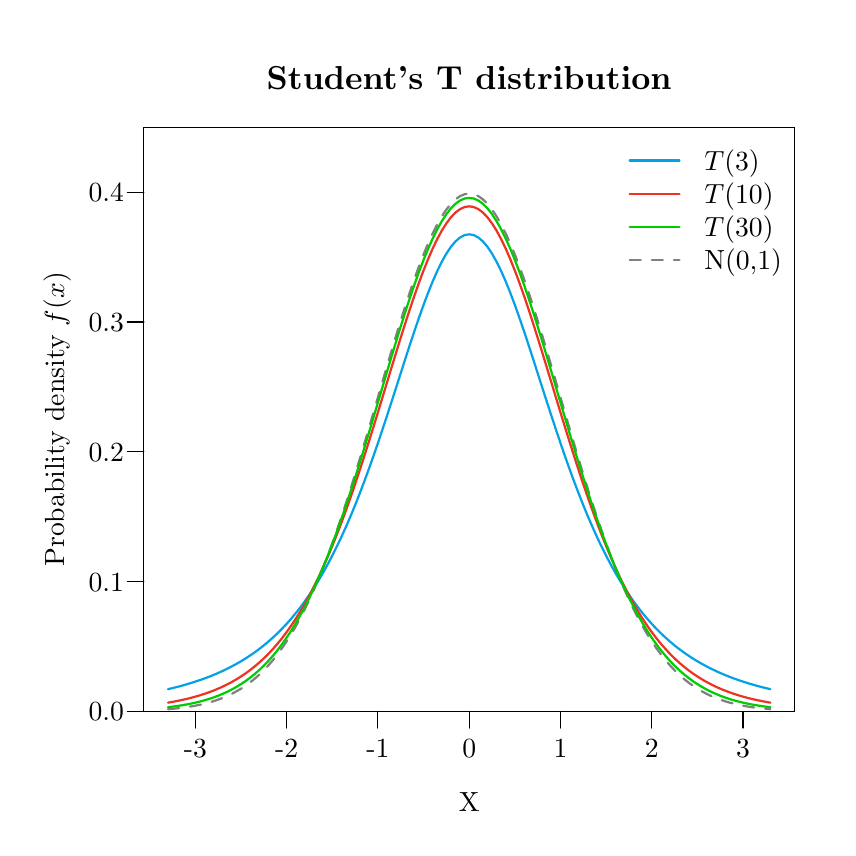
\begin{tikzpicture}[x=1pt,y=1pt]
\definecolor{fillColor}{RGB}{255,255,255}
\path[use as bounding box,fill=fillColor,fill opacity=0.00] (0,0) rectangle (289.08,289.08);
\begin{scope}
\path[clip] ( 42.00, 42.00) rectangle (277.08,253.08);
\definecolor{drawColor}{RGB}{128,128,128}

\path[draw=drawColor,line width= 0.8pt,dash pattern=on 4pt off 4pt ,line join=round,line cap=round] ( 50.71, 42.81) --
	( 52.36, 42.95) --
	( 54.00, 43.12) --
	( 55.65, 43.31) --
	( 57.30, 43.53) --
	( 58.95, 43.79) --
	( 60.60, 44.08) --
	( 62.25, 44.41) --
	( 63.90, 44.79) --
	( 65.55, 45.22) --
	( 67.20, 45.71) --
	( 68.85, 46.27) --
	( 70.49, 46.89) --
	( 72.14, 47.59) --
	( 73.79, 48.37) --
	( 75.44, 49.25) --
	( 77.09, 50.22) --
	( 78.74, 51.31) --
	( 80.39, 52.50) --
	( 82.04, 53.83) --
	( 83.69, 55.29) --
	( 85.34, 56.89) --
	( 86.98, 58.64) --
	( 88.63, 60.55) --
	( 90.28, 62.63) --
	( 91.93, 64.89) --
	( 93.58, 67.33) --
	( 95.23, 69.95) --
	( 96.88, 72.78) --
	( 98.53, 75.80) --
	(100.18, 79.03) --
	(101.83, 82.47) --
	(103.47, 86.12) --
	(105.12, 89.97) --
	(106.77, 94.03) --
	(108.42, 98.29) --
	(110.07,102.75) --
	(111.72,107.40) --
	(113.37,112.23) --
	(115.02,117.23) --
	(116.67,122.38) --
	(118.32,127.67) --
	(119.96,133.09) --
	(121.61,138.60) --
	(123.26,144.19) --
	(124.91,149.83) --
	(126.56,155.50) --
	(128.21,161.17) --
	(129.86,166.81) --
	(131.51,172.39) --
	(133.16,177.88) --
	(134.81,183.25) --
	(136.45,188.47) --
	(138.10,193.50) --
	(139.75,198.30) --
	(141.40,202.86) --
	(143.05,207.14) --
	(144.70,211.11) --
	(146.35,214.74) --
	(148.00,218.01) --
	(149.65,220.90) --
	(151.30,223.37) --
	(152.94,225.43) --
	(154.59,227.04) --
	(156.24,228.20) --
	(157.89,228.90) --
	(159.54,229.13) --
	(161.19,228.90) --
	(162.84,228.20) --
	(164.49,227.04) --
	(166.14,225.43) --
	(167.78,223.37) --
	(169.43,220.90) --
	(171.08,218.01) --
	(172.73,214.74) --
	(174.38,211.11) --
	(176.03,207.14) --
	(177.68,202.86) --
	(179.33,198.30) --
	(180.98,193.50) --
	(182.63,188.47) --
	(184.27,183.25) --
	(185.92,177.88) --
	(187.57,172.39) --
	(189.22,166.81) --
	(190.87,161.17) --
	(192.52,155.50) --
	(194.17,149.83) --
	(195.82,144.19) --
	(197.47,138.60) --
	(199.12,133.09) --
	(200.76,127.67) --
	(202.41,122.38) --
	(204.06,117.23) --
	(205.71,112.23) --
	(207.36,107.40) --
	(209.01,102.75) --
	(210.66, 98.29) --
	(212.31, 94.03) --
	(213.96, 89.97) --
	(215.61, 86.12) --
	(217.25, 82.47) --
	(218.90, 79.03) --
	(220.55, 75.80) --
	(222.20, 72.78) --
	(223.85, 69.95) --
	(225.50, 67.33) --
	(227.15, 64.89) --
	(228.80, 62.63) --
	(230.45, 60.55) --
	(232.10, 58.64) --
	(233.74, 56.89) --
	(235.39, 55.29) --
	(237.04, 53.83) --
	(238.69, 52.50) --
	(240.34, 51.31) --
	(241.99, 50.22) --
	(243.64, 49.25) --
	(245.29, 48.37) --
	(246.94, 47.59) --
	(248.59, 46.89) --
	(250.23, 46.27) --
	(251.88, 45.71) --
	(253.53, 45.22) --
	(255.18, 44.79) --
	(256.83, 44.41) --
	(258.48, 44.08) --
	(260.13, 43.79) --
	(261.78, 43.53) --
	(263.43, 43.31) --
	(265.08, 43.12) --
	(266.72, 42.95) --
	(268.37, 42.81);
\end{scope}
\begin{scope}
\path[clip] (  0.00,  0.00) rectangle (289.08,289.08);
\definecolor{drawColor}{RGB}{0,0,0}

\path[draw=drawColor,line width= 0.4pt,line join=round,line cap=round] ( 60.60, 42.00) -- (258.48, 42.00);

\path[draw=drawColor,line width= 0.4pt,line join=round,line cap=round] ( 60.60, 42.00) -- ( 60.60, 36.00);

\path[draw=drawColor,line width= 0.4pt,line join=round,line cap=round] ( 93.58, 42.00) -- ( 93.58, 36.00);

\path[draw=drawColor,line width= 0.4pt,line join=round,line cap=round] (126.56, 42.00) -- (126.56, 36.00);

\path[draw=drawColor,line width= 0.4pt,line join=round,line cap=round] (159.54, 42.00) -- (159.54, 36.00);

\path[draw=drawColor,line width= 0.4pt,line join=round,line cap=round] (192.52, 42.00) -- (192.52, 36.00);

\path[draw=drawColor,line width= 0.4pt,line join=round,line cap=round] (225.50, 42.00) -- (225.50, 36.00);

\path[draw=drawColor,line width= 0.4pt,line join=round,line cap=round] (258.48, 42.00) -- (258.48, 36.00);

\node[text=drawColor,anchor=base,inner sep=0pt, outer sep=0pt, scale=  1.00] at ( 60.60, 25.20) {-3};

\node[text=drawColor,anchor=base,inner sep=0pt, outer sep=0pt, scale=  1.00] at ( 93.58, 25.20) {-2};

\node[text=drawColor,anchor=base,inner sep=0pt, outer sep=0pt, scale=  1.00] at (126.56, 25.20) {-1};

\node[text=drawColor,anchor=base,inner sep=0pt, outer sep=0pt, scale=  1.00] at (159.54, 25.20) {0};

\node[text=drawColor,anchor=base,inner sep=0pt, outer sep=0pt, scale=  1.00] at (192.52, 25.20) {1};

\node[text=drawColor,anchor=base,inner sep=0pt, outer sep=0pt, scale=  1.00] at (225.50, 25.20) {2};

\node[text=drawColor,anchor=base,inner sep=0pt, outer sep=0pt, scale=  1.00] at (258.48, 25.20) {3};

\path[draw=drawColor,line width= 0.4pt,line join=round,line cap=round] ( 42.00, 42.00) -- ( 42.00,229.63);

\path[draw=drawColor,line width= 0.4pt,line join=round,line cap=round] ( 42.00, 42.00) -- ( 36.00, 42.00);

\path[draw=drawColor,line width= 0.4pt,line join=round,line cap=round] ( 42.00, 88.91) -- ( 36.00, 88.91);

\path[draw=drawColor,line width= 0.4pt,line join=round,line cap=round] ( 42.00,135.81) -- ( 36.00,135.81);

\path[draw=drawColor,line width= 0.4pt,line join=round,line cap=round] ( 42.00,182.72) -- ( 36.00,182.72);

\path[draw=drawColor,line width= 0.4pt,line join=round,line cap=round] ( 42.00,229.63) -- ( 36.00,229.63);

\node[text=drawColor,anchor=base east,inner sep=0pt, outer sep=0pt, scale=  1.00] at ( 34.80, 38.56) {0.0};

\node[text=drawColor,anchor=base east,inner sep=0pt, outer sep=0pt, scale=  1.00] at ( 34.80, 85.46) {0.1};

\node[text=drawColor,anchor=base east,inner sep=0pt, outer sep=0pt, scale=  1.00] at ( 34.80,132.37) {0.2};

\node[text=drawColor,anchor=base east,inner sep=0pt, outer sep=0pt, scale=  1.00] at ( 34.80,179.28) {0.3};

\node[text=drawColor,anchor=base east,inner sep=0pt, outer sep=0pt, scale=  1.00] at ( 34.80,226.18) {0.4};

\path[draw=drawColor,line width= 0.4pt,line join=round,line cap=round] ( 42.00, 42.00) --
	(277.08, 42.00) --
	(277.08,253.08) --
	( 42.00,253.08) --
	( 42.00, 42.00);
\end{scope}
\begin{scope}
\path[clip] (  0.00,  0.00) rectangle (289.08,289.08);
\definecolor{drawColor}{RGB}{0,0,0}

\node[text=drawColor,anchor=base,inner sep=0pt, outer sep=0pt, scale=  1.20] at (159.54,266.89) {\bfseries Student's T distribution};

\node[text=drawColor,anchor=base,inner sep=0pt, outer sep=0pt, scale=  1.00] at (159.54,  6.00) {X};

\node[text=drawColor,rotate= 90.00,anchor=base,inner sep=0pt, outer sep=0pt, scale=  1.00] at ( 13.20,147.54) {Probability density $f(x)$};
\end{scope}
\begin{scope}
\path[clip] ( 42.00, 42.00) rectangle (277.08,253.08);
\definecolor{drawColor}{RGB}{5,161,230}

\path[draw=drawColor,line width= 0.8pt,line join=round,line cap=round] ( 50.71, 50.04) --
	( 52.36, 50.44) --
	( 54.00, 50.85) --
	( 55.65, 51.29) --
	( 57.30, 51.76) --
	( 58.95, 52.25) --
	( 60.60, 52.78) --
	( 62.25, 53.33) --
	( 63.90, 53.92) --
	( 65.55, 54.54) --
	( 67.20, 55.20) --
	( 68.85, 55.91) --
	( 70.49, 56.65) --
	( 72.14, 57.45) --
	( 73.79, 58.29) --
	( 75.44, 59.18) --
	( 77.09, 60.13) --
	( 78.74, 61.15) --
	( 80.39, 62.22) --
	( 82.04, 63.36) --
	( 83.69, 64.58) --
	( 85.34, 65.87) --
	( 86.98, 67.24) --
	( 88.63, 68.71) --
	( 90.28, 70.26) --
	( 91.93, 71.91) --
	( 93.58, 73.67) --
	( 95.23, 75.53) --
	( 96.88, 77.51) --
	( 98.53, 79.62) --
	(100.18, 81.85) --
	(101.83, 84.22) --
	(103.47, 86.73) --
	(105.12, 89.38) --
	(106.77, 92.19) --
	(108.42, 95.16) --
	(110.07, 98.30) --
	(111.72,101.60) --
	(113.37,105.07) --
	(115.02,108.72) --
	(116.67,112.54) --
	(118.32,116.54) --
	(119.96,120.71) --
	(121.61,125.05) --
	(123.26,129.55) --
	(124.91,134.19) --
	(126.56,138.98) --
	(128.21,143.89) --
	(129.86,148.89) --
	(131.51,153.98) --
	(133.16,159.11) --
	(134.81,164.26) --
	(136.45,169.39) --
	(138.10,174.47) --
	(139.75,179.44) --
	(141.40,184.27) --
	(143.05,188.90) --
	(144.70,193.29) --
	(146.35,197.39) --
	(148.00,201.14) --
	(149.65,204.51) --
	(151.30,207.44) --
	(152.94,209.90) --
	(154.59,211.85) --
	(156.24,213.26) --
	(157.89,214.12) --
	(159.54,214.41) --
	(161.19,214.12) --
	(162.84,213.26) --
	(164.49,211.85) --
	(166.14,209.90) --
	(167.78,207.44) --
	(169.43,204.51) --
	(171.08,201.14) --
	(172.73,197.39) --
	(174.38,193.29) --
	(176.03,188.90) --
	(177.68,184.27) --
	(179.33,179.44) --
	(180.98,174.47) --
	(182.63,169.39) --
	(184.27,164.26) --
	(185.92,159.11) --
	(187.57,153.98) --
	(189.22,148.89) --
	(190.87,143.89) --
	(192.52,138.98) --
	(194.17,134.19) --
	(195.82,129.55) --
	(197.47,125.05) --
	(199.12,120.71) --
	(200.76,116.54) --
	(202.41,112.54) --
	(204.06,108.72) --
	(205.71,105.07) --
	(207.36,101.60) --
	(209.01, 98.30) --
	(210.66, 95.16) --
	(212.31, 92.19) --
	(213.96, 89.38) --
	(215.61, 86.73) --
	(217.25, 84.22) --
	(218.90, 81.85) --
	(220.55, 79.62) --
	(222.20, 77.51) --
	(223.85, 75.53) --
	(225.50, 73.67) --
	(227.15, 71.91) --
	(228.80, 70.26) --
	(230.45, 68.71) --
	(232.10, 67.24) --
	(233.74, 65.87) --
	(235.39, 64.58) --
	(237.04, 63.36) --
	(238.69, 62.22) --
	(240.34, 61.15) --
	(241.99, 60.13) --
	(243.64, 59.18) --
	(245.29, 58.29) --
	(246.94, 57.45) --
	(248.59, 56.65) --
	(250.23, 55.91) --
	(251.88, 55.20) --
	(253.53, 54.54) --
	(255.18, 53.92) --
	(256.83, 53.33) --
	(258.48, 52.78) --
	(260.13, 52.25) --
	(261.78, 51.76) --
	(263.43, 51.29) --
	(265.08, 50.85) --
	(266.72, 50.44) --
	(268.37, 50.04);
\definecolor{drawColor}{RGB}{238,50,36}

\path[draw=drawColor,line width= 0.8pt,line join=round,line cap=round] ( 50.71, 45.17) --
	( 52.36, 45.46) --
	( 54.00, 45.78) --
	( 55.65, 46.12) --
	( 57.30, 46.49) --
	( 58.95, 46.90) --
	( 60.60, 47.35) --
	( 62.25, 47.83) --
	( 63.90, 48.36) --
	( 65.55, 48.94) --
	( 67.20, 49.56) --
	( 68.85, 50.24) --
	( 70.49, 50.98) --
	( 72.14, 51.79) --
	( 73.79, 52.66) --
	( 75.44, 53.61) --
	( 77.09, 54.64) --
	( 78.74, 55.75) --
	( 80.39, 56.95) --
	( 82.04, 58.26) --
	( 83.69, 59.66) --
	( 85.34, 61.18) --
	( 86.98, 62.82) --
	( 88.63, 64.58) --
	( 90.28, 66.47) --
	( 91.93, 68.50) --
	( 93.58, 70.68) --
	( 95.23, 73.01) --
	( 96.88, 75.50) --
	( 98.53, 78.16) --
	(100.18, 80.99) --
	(101.83, 83.99) --
	(103.47, 87.18) --
	(105.12, 90.55) --
	(106.77, 94.10) --
	(108.42, 97.85) --
	(110.07,101.78) --
	(111.72,105.90) --
	(113.37,110.20) --
	(115.02,114.68) --
	(116.67,119.33) --
	(118.32,124.13) --
	(119.96,129.09) --
	(121.61,134.18) --
	(123.26,139.38) --
	(124.91,144.68) --
	(126.56,150.06) --
	(128.21,155.48) --
	(129.86,160.92) --
	(131.51,166.36) --
	(133.16,171.76) --
	(134.81,177.08) --
	(136.45,182.29) --
	(138.10,187.36) --
	(139.75,192.25) --
	(141.40,196.92) --
	(143.05,201.34) --
	(144.70,205.46) --
	(146.35,209.26) --
	(148.00,212.70) --
	(149.65,215.74) --
	(151.30,218.37) --
	(152.94,220.55) --
	(154.59,222.28) --
	(156.24,223.52) --
	(157.89,224.27) --
	(159.54,224.52) --
	(161.19,224.27) --
	(162.84,223.52) --
	(164.49,222.28) --
	(166.14,220.55) --
	(167.78,218.37) --
	(169.43,215.74) --
	(171.08,212.70) --
	(172.73,209.26) --
	(174.38,205.46) --
	(176.03,201.34) --
	(177.68,196.92) --
	(179.33,192.25) --
	(180.98,187.36) --
	(182.63,182.29) --
	(184.27,177.08) --
	(185.92,171.76) --
	(187.57,166.36) --
	(189.22,160.92) --
	(190.87,155.48) --
	(192.52,150.06) --
	(194.17,144.68) --
	(195.82,139.38) --
	(197.47,134.18) --
	(199.12,129.09) --
	(200.76,124.13) --
	(202.41,119.33) --
	(204.06,114.68) --
	(205.71,110.20) --
	(207.36,105.90) --
	(209.01,101.78) --
	(210.66, 97.85) --
	(212.31, 94.10) --
	(213.96, 90.55) --
	(215.61, 87.18) --
	(217.25, 83.99) --
	(218.90, 80.99) --
	(220.55, 78.16) --
	(222.20, 75.50) --
	(223.85, 73.01) --
	(225.50, 70.68) --
	(227.15, 68.50) --
	(228.80, 66.47) --
	(230.45, 64.58) --
	(232.10, 62.82) --
	(233.74, 61.18) --
	(235.39, 59.66) --
	(237.04, 58.26) --
	(238.69, 56.95) --
	(240.34, 55.75) --
	(241.99, 54.64) --
	(243.64, 53.61) --
	(245.29, 52.66) --
	(246.94, 51.79) --
	(248.59, 50.98) --
	(250.23, 50.24) --
	(251.88, 49.56) --
	(253.53, 48.94) --
	(255.18, 48.36) --
	(256.83, 47.83) --
	(258.48, 47.35) --
	(260.13, 46.90) --
	(261.78, 46.49) --
	(263.43, 46.12) --
	(265.08, 45.78) --
	(266.72, 45.46) --
	(268.37, 45.17);
\definecolor{drawColor}{RGB}{0,205,0}

\path[draw=drawColor,line width= 0.8pt,line join=round,line cap=round] ( 50.71, 43.53) --
	( 52.36, 43.73) --
	( 54.00, 43.96) --
	( 55.65, 44.21) --
	( 57.30, 44.50) --
	( 58.95, 44.82) --
	( 60.60, 45.18) --
	( 62.25, 45.58) --
	( 63.90, 46.03) --
	( 65.55, 46.52) --
	( 67.20, 47.08) --
	( 68.85, 47.69) --
	( 70.49, 48.37) --
	( 72.14, 49.12) --
	( 73.79, 49.95) --
	( 75.44, 50.87) --
	( 77.09, 51.88) --
	( 78.74, 52.98) --
	( 80.39, 54.20) --
	( 82.04, 55.52) --
	( 83.69, 56.97) --
	( 85.34, 58.55) --
	( 86.98, 60.27) --
	( 88.63, 62.13) --
	( 90.28, 64.15) --
	( 91.93, 66.32) --
	( 93.58, 68.67) --
	( 95.23, 71.19) --
	( 96.88, 73.89) --
	( 98.53, 76.78) --
	(100.18, 79.86) --
	(101.83, 83.13) --
	(103.47, 86.61) --
	(105.12, 90.28) --
	(106.77, 94.16) --
	(108.42, 98.23) --
	(110.07,102.49) --
	(111.72,106.95) --
	(113.37,111.58) --
	(115.02,116.39) --
	(116.67,121.36) --
	(118.32,126.48) --
	(119.96,131.73) --
	(121.61,137.09) --
	(123.26,142.54) --
	(124.91,148.07) --
	(126.56,153.63) --
	(128.21,159.22) --
	(129.86,164.80) --
	(131.51,170.33) --
	(133.16,175.79) --
	(134.81,181.15) --
	(136.45,186.37) --
	(138.10,191.41) --
	(139.75,196.25) --
	(141.40,200.85) --
	(143.05,205.18) --
	(144.70,209.20) --
	(146.35,212.89) --
	(148.00,216.22) --
	(149.65,219.16) --
	(151.30,221.69) --
	(152.94,223.78) --
	(154.59,225.43) --
	(156.24,226.62) --
	(157.89,227.34) --
	(159.54,227.58) --
	(161.19,227.34) --
	(162.84,226.62) --
	(164.49,225.43) --
	(166.14,223.78) --
	(167.78,221.69) --
	(169.43,219.16) --
	(171.08,216.22) --
	(172.73,212.89) --
	(174.38,209.20) --
	(176.03,205.18) --
	(177.68,200.85) --
	(179.33,196.25) --
	(180.98,191.41) --
	(182.63,186.37) --
	(184.27,181.15) --
	(185.92,175.79) --
	(187.57,170.33) --
	(189.22,164.80) --
	(190.87,159.22) --
	(192.52,153.63) --
	(194.17,148.07) --
	(195.82,142.54) --
	(197.47,137.09) --
	(199.12,131.73) --
	(200.76,126.48) --
	(202.41,121.36) --
	(204.06,116.39) --
	(205.71,111.58) --
	(207.36,106.95) --
	(209.01,102.49) --
	(210.66, 98.23) --
	(212.31, 94.16) --
	(213.96, 90.28) --
	(215.61, 86.61) --
	(217.25, 83.13) --
	(218.90, 79.86) --
	(220.55, 76.78) --
	(222.20, 73.89) --
	(223.85, 71.19) --
	(225.50, 68.67) --
	(227.15, 66.32) --
	(228.80, 64.15) --
	(230.45, 62.13) --
	(232.10, 60.27) --
	(233.74, 58.55) --
	(235.39, 56.97) --
	(237.04, 55.52) --
	(238.69, 54.20) --
	(240.34, 52.98) --
	(241.99, 51.88) --
	(243.64, 50.87) --
	(245.29, 49.95) --
	(246.94, 49.12) --
	(248.59, 48.37) --
	(250.23, 47.69) --
	(251.88, 47.08) --
	(253.53, 46.52) --
	(255.18, 46.03) --
	(256.83, 45.58) --
	(258.48, 45.18) --
	(260.13, 44.82) --
	(261.78, 44.50) --
	(263.43, 44.21) --
	(265.08, 43.96) --
	(266.72, 43.73) --
	(268.37, 43.53);
\definecolor{drawColor}{RGB}{5,161,230}

\path[draw=drawColor,line width= 0.8pt,line join=round,line cap=round] (217.52,241.08) -- (235.52,241.08);
\definecolor{drawColor}{RGB}{238,50,36}

\path[draw=drawColor,line width= 0.8pt,line join=round,line cap=round] (217.52,229.08) -- (235.52,229.08);
\definecolor{drawColor}{RGB}{0,205,0}

\path[draw=drawColor,line width= 0.8pt,line join=round,line cap=round] (217.52,217.08) -- (235.52,217.08);
\definecolor{drawColor}{RGB}{128,128,128}

\path[draw=drawColor,line width= 0.8pt,dash pattern=on 4pt off 4pt ,line join=round,line cap=round] (217.52,205.08) -- (235.52,205.08);
\definecolor{drawColor}{RGB}{0,0,0}

\node[text=drawColor,anchor=base west,inner sep=0pt, outer sep=0pt, scale=  1.00] at (244.52,237.64) {$T(3)$};

\node[text=drawColor,anchor=base west,inner sep=0pt, outer sep=0pt, scale=  1.00] at (244.52,225.64) {$T(10)$};

\node[text=drawColor,anchor=base west,inner sep=0pt, outer sep=0pt, scale=  1.00] at (244.52,213.64) {$T(30)$};

\node[text=drawColor,anchor=base west,inner sep=0pt, outer sep=0pt, scale=  1.00] at (244.52,201.64) {N(0,1)};
\end{scope}
\begin{scope}
\path[clip] (  0.00,  0.00) rectangle (289.08,289.08);
\definecolor{drawColor}{RGB}{0,0,0}

\path[draw=drawColor,line width= 0.4pt,line join=round,line cap=round] ( 42.00, 42.00) --
	(277.08, 42.00) --
	(277.08,253.08) --
	( 42.00,253.08) --
	( 42.00, 42.00);
\end{scope}
\end{tikzpicture}
}}
\mode<presentation>{\resizebox{0.6\textwidth}{!}{% Created by tikzDevice version 0.10.1 on 2016-05-09 15:28:50
% !TEX encoding = UTF-8 Unicode
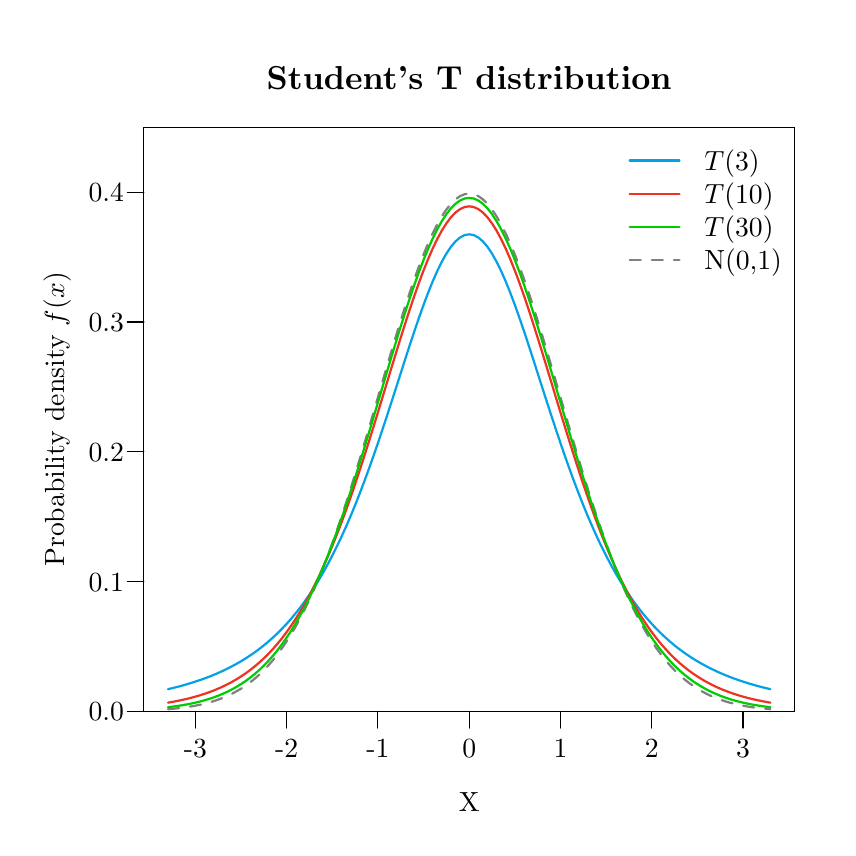
\begin{tikzpicture}[x=1pt,y=1pt]
\definecolor{fillColor}{RGB}{255,255,255}
\path[use as bounding box,fill=fillColor,fill opacity=0.00] (0,0) rectangle (289.08,289.08);
\begin{scope}
\path[clip] ( 42.00, 42.00) rectangle (277.08,253.08);
\definecolor{drawColor}{RGB}{128,128,128}

\path[draw=drawColor,line width= 0.8pt,dash pattern=on 4pt off 4pt ,line join=round,line cap=round] ( 50.71, 42.81) --
	( 52.36, 42.95) --
	( 54.00, 43.12) --
	( 55.65, 43.31) --
	( 57.30, 43.53) --
	( 58.95, 43.79) --
	( 60.60, 44.08) --
	( 62.25, 44.41) --
	( 63.90, 44.79) --
	( 65.55, 45.22) --
	( 67.20, 45.71) --
	( 68.85, 46.27) --
	( 70.49, 46.89) --
	( 72.14, 47.59) --
	( 73.79, 48.37) --
	( 75.44, 49.25) --
	( 77.09, 50.22) --
	( 78.74, 51.31) --
	( 80.39, 52.50) --
	( 82.04, 53.83) --
	( 83.69, 55.29) --
	( 85.34, 56.89) --
	( 86.98, 58.64) --
	( 88.63, 60.55) --
	( 90.28, 62.63) --
	( 91.93, 64.89) --
	( 93.58, 67.33) --
	( 95.23, 69.95) --
	( 96.88, 72.78) --
	( 98.53, 75.80) --
	(100.18, 79.03) --
	(101.83, 82.47) --
	(103.47, 86.12) --
	(105.12, 89.97) --
	(106.77, 94.03) --
	(108.42, 98.29) --
	(110.07,102.75) --
	(111.72,107.40) --
	(113.37,112.23) --
	(115.02,117.23) --
	(116.67,122.38) --
	(118.32,127.67) --
	(119.96,133.09) --
	(121.61,138.60) --
	(123.26,144.19) --
	(124.91,149.83) --
	(126.56,155.50) --
	(128.21,161.17) --
	(129.86,166.81) --
	(131.51,172.39) --
	(133.16,177.88) --
	(134.81,183.25) --
	(136.45,188.47) --
	(138.10,193.50) --
	(139.75,198.30) --
	(141.40,202.86) --
	(143.05,207.14) --
	(144.70,211.11) --
	(146.35,214.74) --
	(148.00,218.01) --
	(149.65,220.90) --
	(151.30,223.37) --
	(152.94,225.43) --
	(154.59,227.04) --
	(156.24,228.20) --
	(157.89,228.90) --
	(159.54,229.13) --
	(161.19,228.90) --
	(162.84,228.20) --
	(164.49,227.04) --
	(166.14,225.43) --
	(167.78,223.37) --
	(169.43,220.90) --
	(171.08,218.01) --
	(172.73,214.74) --
	(174.38,211.11) --
	(176.03,207.14) --
	(177.68,202.86) --
	(179.33,198.30) --
	(180.98,193.50) --
	(182.63,188.47) --
	(184.27,183.25) --
	(185.92,177.88) --
	(187.57,172.39) --
	(189.22,166.81) --
	(190.87,161.17) --
	(192.52,155.50) --
	(194.17,149.83) --
	(195.82,144.19) --
	(197.47,138.60) --
	(199.12,133.09) --
	(200.76,127.67) --
	(202.41,122.38) --
	(204.06,117.23) --
	(205.71,112.23) --
	(207.36,107.40) --
	(209.01,102.75) --
	(210.66, 98.29) --
	(212.31, 94.03) --
	(213.96, 89.97) --
	(215.61, 86.12) --
	(217.25, 82.47) --
	(218.90, 79.03) --
	(220.55, 75.80) --
	(222.20, 72.78) --
	(223.85, 69.95) --
	(225.50, 67.33) --
	(227.15, 64.89) --
	(228.80, 62.63) --
	(230.45, 60.55) --
	(232.10, 58.64) --
	(233.74, 56.89) --
	(235.39, 55.29) --
	(237.04, 53.83) --
	(238.69, 52.50) --
	(240.34, 51.31) --
	(241.99, 50.22) --
	(243.64, 49.25) --
	(245.29, 48.37) --
	(246.94, 47.59) --
	(248.59, 46.89) --
	(250.23, 46.27) --
	(251.88, 45.71) --
	(253.53, 45.22) --
	(255.18, 44.79) --
	(256.83, 44.41) --
	(258.48, 44.08) --
	(260.13, 43.79) --
	(261.78, 43.53) --
	(263.43, 43.31) --
	(265.08, 43.12) --
	(266.72, 42.95) --
	(268.37, 42.81);
\end{scope}
\begin{scope}
\path[clip] (  0.00,  0.00) rectangle (289.08,289.08);
\definecolor{drawColor}{RGB}{0,0,0}

\path[draw=drawColor,line width= 0.4pt,line join=round,line cap=round] ( 60.60, 42.00) -- (258.48, 42.00);

\path[draw=drawColor,line width= 0.4pt,line join=round,line cap=round] ( 60.60, 42.00) -- ( 60.60, 36.00);

\path[draw=drawColor,line width= 0.4pt,line join=round,line cap=round] ( 93.58, 42.00) -- ( 93.58, 36.00);

\path[draw=drawColor,line width= 0.4pt,line join=round,line cap=round] (126.56, 42.00) -- (126.56, 36.00);

\path[draw=drawColor,line width= 0.4pt,line join=round,line cap=round] (159.54, 42.00) -- (159.54, 36.00);

\path[draw=drawColor,line width= 0.4pt,line join=round,line cap=round] (192.52, 42.00) -- (192.52, 36.00);

\path[draw=drawColor,line width= 0.4pt,line join=round,line cap=round] (225.50, 42.00) -- (225.50, 36.00);

\path[draw=drawColor,line width= 0.4pt,line join=round,line cap=round] (258.48, 42.00) -- (258.48, 36.00);

\node[text=drawColor,anchor=base,inner sep=0pt, outer sep=0pt, scale=  1.00] at ( 60.60, 25.20) {-3};

\node[text=drawColor,anchor=base,inner sep=0pt, outer sep=0pt, scale=  1.00] at ( 93.58, 25.20) {-2};

\node[text=drawColor,anchor=base,inner sep=0pt, outer sep=0pt, scale=  1.00] at (126.56, 25.20) {-1};

\node[text=drawColor,anchor=base,inner sep=0pt, outer sep=0pt, scale=  1.00] at (159.54, 25.20) {0};

\node[text=drawColor,anchor=base,inner sep=0pt, outer sep=0pt, scale=  1.00] at (192.52, 25.20) {1};

\node[text=drawColor,anchor=base,inner sep=0pt, outer sep=0pt, scale=  1.00] at (225.50, 25.20) {2};

\node[text=drawColor,anchor=base,inner sep=0pt, outer sep=0pt, scale=  1.00] at (258.48, 25.20) {3};

\path[draw=drawColor,line width= 0.4pt,line join=round,line cap=round] ( 42.00, 42.00) -- ( 42.00,229.63);

\path[draw=drawColor,line width= 0.4pt,line join=round,line cap=round] ( 42.00, 42.00) -- ( 36.00, 42.00);

\path[draw=drawColor,line width= 0.4pt,line join=round,line cap=round] ( 42.00, 88.91) -- ( 36.00, 88.91);

\path[draw=drawColor,line width= 0.4pt,line join=round,line cap=round] ( 42.00,135.81) -- ( 36.00,135.81);

\path[draw=drawColor,line width= 0.4pt,line join=round,line cap=round] ( 42.00,182.72) -- ( 36.00,182.72);

\path[draw=drawColor,line width= 0.4pt,line join=round,line cap=round] ( 42.00,229.63) -- ( 36.00,229.63);

\node[text=drawColor,anchor=base east,inner sep=0pt, outer sep=0pt, scale=  1.00] at ( 34.80, 38.56) {0.0};

\node[text=drawColor,anchor=base east,inner sep=0pt, outer sep=0pt, scale=  1.00] at ( 34.80, 85.46) {0.1};

\node[text=drawColor,anchor=base east,inner sep=0pt, outer sep=0pt, scale=  1.00] at ( 34.80,132.37) {0.2};

\node[text=drawColor,anchor=base east,inner sep=0pt, outer sep=0pt, scale=  1.00] at ( 34.80,179.28) {0.3};

\node[text=drawColor,anchor=base east,inner sep=0pt, outer sep=0pt, scale=  1.00] at ( 34.80,226.18) {0.4};

\path[draw=drawColor,line width= 0.4pt,line join=round,line cap=round] ( 42.00, 42.00) --
	(277.08, 42.00) --
	(277.08,253.08) --
	( 42.00,253.08) --
	( 42.00, 42.00);
\end{scope}
\begin{scope}
\path[clip] (  0.00,  0.00) rectangle (289.08,289.08);
\definecolor{drawColor}{RGB}{0,0,0}

\node[text=drawColor,anchor=base,inner sep=0pt, outer sep=0pt, scale=  1.20] at (159.54,266.89) {\bfseries Student's T distribution};

\node[text=drawColor,anchor=base,inner sep=0pt, outer sep=0pt, scale=  1.00] at (159.54,  6.00) {X};

\node[text=drawColor,rotate= 90.00,anchor=base,inner sep=0pt, outer sep=0pt, scale=  1.00] at ( 13.20,147.54) {Probability density $f(x)$};
\end{scope}
\begin{scope}
\path[clip] ( 42.00, 42.00) rectangle (277.08,253.08);
\definecolor{drawColor}{RGB}{5,161,230}

\path[draw=drawColor,line width= 0.8pt,line join=round,line cap=round] ( 50.71, 50.04) --
	( 52.36, 50.44) --
	( 54.00, 50.85) --
	( 55.65, 51.29) --
	( 57.30, 51.76) --
	( 58.95, 52.25) --
	( 60.60, 52.78) --
	( 62.25, 53.33) --
	( 63.90, 53.92) --
	( 65.55, 54.54) --
	( 67.20, 55.20) --
	( 68.85, 55.91) --
	( 70.49, 56.65) --
	( 72.14, 57.45) --
	( 73.79, 58.29) --
	( 75.44, 59.18) --
	( 77.09, 60.13) --
	( 78.74, 61.15) --
	( 80.39, 62.22) --
	( 82.04, 63.36) --
	( 83.69, 64.58) --
	( 85.34, 65.87) --
	( 86.98, 67.24) --
	( 88.63, 68.71) --
	( 90.28, 70.26) --
	( 91.93, 71.91) --
	( 93.58, 73.67) --
	( 95.23, 75.53) --
	( 96.88, 77.51) --
	( 98.53, 79.62) --
	(100.18, 81.85) --
	(101.83, 84.22) --
	(103.47, 86.73) --
	(105.12, 89.38) --
	(106.77, 92.19) --
	(108.42, 95.16) --
	(110.07, 98.30) --
	(111.72,101.60) --
	(113.37,105.07) --
	(115.02,108.72) --
	(116.67,112.54) --
	(118.32,116.54) --
	(119.96,120.71) --
	(121.61,125.05) --
	(123.26,129.55) --
	(124.91,134.19) --
	(126.56,138.98) --
	(128.21,143.89) --
	(129.86,148.89) --
	(131.51,153.98) --
	(133.16,159.11) --
	(134.81,164.26) --
	(136.45,169.39) --
	(138.10,174.47) --
	(139.75,179.44) --
	(141.40,184.27) --
	(143.05,188.90) --
	(144.70,193.29) --
	(146.35,197.39) --
	(148.00,201.14) --
	(149.65,204.51) --
	(151.30,207.44) --
	(152.94,209.90) --
	(154.59,211.85) --
	(156.24,213.26) --
	(157.89,214.12) --
	(159.54,214.41) --
	(161.19,214.12) --
	(162.84,213.26) --
	(164.49,211.85) --
	(166.14,209.90) --
	(167.78,207.44) --
	(169.43,204.51) --
	(171.08,201.14) --
	(172.73,197.39) --
	(174.38,193.29) --
	(176.03,188.90) --
	(177.68,184.27) --
	(179.33,179.44) --
	(180.98,174.47) --
	(182.63,169.39) --
	(184.27,164.26) --
	(185.92,159.11) --
	(187.57,153.98) --
	(189.22,148.89) --
	(190.87,143.89) --
	(192.52,138.98) --
	(194.17,134.19) --
	(195.82,129.55) --
	(197.47,125.05) --
	(199.12,120.71) --
	(200.76,116.54) --
	(202.41,112.54) --
	(204.06,108.72) --
	(205.71,105.07) --
	(207.36,101.60) --
	(209.01, 98.30) --
	(210.66, 95.16) --
	(212.31, 92.19) --
	(213.96, 89.38) --
	(215.61, 86.73) --
	(217.25, 84.22) --
	(218.90, 81.85) --
	(220.55, 79.62) --
	(222.20, 77.51) --
	(223.85, 75.53) --
	(225.50, 73.67) --
	(227.15, 71.91) --
	(228.80, 70.26) --
	(230.45, 68.71) --
	(232.10, 67.24) --
	(233.74, 65.87) --
	(235.39, 64.58) --
	(237.04, 63.36) --
	(238.69, 62.22) --
	(240.34, 61.15) --
	(241.99, 60.13) --
	(243.64, 59.18) --
	(245.29, 58.29) --
	(246.94, 57.45) --
	(248.59, 56.65) --
	(250.23, 55.91) --
	(251.88, 55.20) --
	(253.53, 54.54) --
	(255.18, 53.92) --
	(256.83, 53.33) --
	(258.48, 52.78) --
	(260.13, 52.25) --
	(261.78, 51.76) --
	(263.43, 51.29) --
	(265.08, 50.85) --
	(266.72, 50.44) --
	(268.37, 50.04);
\definecolor{drawColor}{RGB}{238,50,36}

\path[draw=drawColor,line width= 0.8pt,line join=round,line cap=round] ( 50.71, 45.17) --
	( 52.36, 45.46) --
	( 54.00, 45.78) --
	( 55.65, 46.12) --
	( 57.30, 46.49) --
	( 58.95, 46.90) --
	( 60.60, 47.35) --
	( 62.25, 47.83) --
	( 63.90, 48.36) --
	( 65.55, 48.94) --
	( 67.20, 49.56) --
	( 68.85, 50.24) --
	( 70.49, 50.98) --
	( 72.14, 51.79) --
	( 73.79, 52.66) --
	( 75.44, 53.61) --
	( 77.09, 54.64) --
	( 78.74, 55.75) --
	( 80.39, 56.95) --
	( 82.04, 58.26) --
	( 83.69, 59.66) --
	( 85.34, 61.18) --
	( 86.98, 62.82) --
	( 88.63, 64.58) --
	( 90.28, 66.47) --
	( 91.93, 68.50) --
	( 93.58, 70.68) --
	( 95.23, 73.01) --
	( 96.88, 75.50) --
	( 98.53, 78.16) --
	(100.18, 80.99) --
	(101.83, 83.99) --
	(103.47, 87.18) --
	(105.12, 90.55) --
	(106.77, 94.10) --
	(108.42, 97.85) --
	(110.07,101.78) --
	(111.72,105.90) --
	(113.37,110.20) --
	(115.02,114.68) --
	(116.67,119.33) --
	(118.32,124.13) --
	(119.96,129.09) --
	(121.61,134.18) --
	(123.26,139.38) --
	(124.91,144.68) --
	(126.56,150.06) --
	(128.21,155.48) --
	(129.86,160.92) --
	(131.51,166.36) --
	(133.16,171.76) --
	(134.81,177.08) --
	(136.45,182.29) --
	(138.10,187.36) --
	(139.75,192.25) --
	(141.40,196.92) --
	(143.05,201.34) --
	(144.70,205.46) --
	(146.35,209.26) --
	(148.00,212.70) --
	(149.65,215.74) --
	(151.30,218.37) --
	(152.94,220.55) --
	(154.59,222.28) --
	(156.24,223.52) --
	(157.89,224.27) --
	(159.54,224.52) --
	(161.19,224.27) --
	(162.84,223.52) --
	(164.49,222.28) --
	(166.14,220.55) --
	(167.78,218.37) --
	(169.43,215.74) --
	(171.08,212.70) --
	(172.73,209.26) --
	(174.38,205.46) --
	(176.03,201.34) --
	(177.68,196.92) --
	(179.33,192.25) --
	(180.98,187.36) --
	(182.63,182.29) --
	(184.27,177.08) --
	(185.92,171.76) --
	(187.57,166.36) --
	(189.22,160.92) --
	(190.87,155.48) --
	(192.52,150.06) --
	(194.17,144.68) --
	(195.82,139.38) --
	(197.47,134.18) --
	(199.12,129.09) --
	(200.76,124.13) --
	(202.41,119.33) --
	(204.06,114.68) --
	(205.71,110.20) --
	(207.36,105.90) --
	(209.01,101.78) --
	(210.66, 97.85) --
	(212.31, 94.10) --
	(213.96, 90.55) --
	(215.61, 87.18) --
	(217.25, 83.99) --
	(218.90, 80.99) --
	(220.55, 78.16) --
	(222.20, 75.50) --
	(223.85, 73.01) --
	(225.50, 70.68) --
	(227.15, 68.50) --
	(228.80, 66.47) --
	(230.45, 64.58) --
	(232.10, 62.82) --
	(233.74, 61.18) --
	(235.39, 59.66) --
	(237.04, 58.26) --
	(238.69, 56.95) --
	(240.34, 55.75) --
	(241.99, 54.64) --
	(243.64, 53.61) --
	(245.29, 52.66) --
	(246.94, 51.79) --
	(248.59, 50.98) --
	(250.23, 50.24) --
	(251.88, 49.56) --
	(253.53, 48.94) --
	(255.18, 48.36) --
	(256.83, 47.83) --
	(258.48, 47.35) --
	(260.13, 46.90) --
	(261.78, 46.49) --
	(263.43, 46.12) --
	(265.08, 45.78) --
	(266.72, 45.46) --
	(268.37, 45.17);
\definecolor{drawColor}{RGB}{0,205,0}

\path[draw=drawColor,line width= 0.8pt,line join=round,line cap=round] ( 50.71, 43.53) --
	( 52.36, 43.73) --
	( 54.00, 43.96) --
	( 55.65, 44.21) --
	( 57.30, 44.50) --
	( 58.95, 44.82) --
	( 60.60, 45.18) --
	( 62.25, 45.58) --
	( 63.90, 46.03) --
	( 65.55, 46.52) --
	( 67.20, 47.08) --
	( 68.85, 47.69) --
	( 70.49, 48.37) --
	( 72.14, 49.12) --
	( 73.79, 49.95) --
	( 75.44, 50.87) --
	( 77.09, 51.88) --
	( 78.74, 52.98) --
	( 80.39, 54.20) --
	( 82.04, 55.52) --
	( 83.69, 56.97) --
	( 85.34, 58.55) --
	( 86.98, 60.27) --
	( 88.63, 62.13) --
	( 90.28, 64.15) --
	( 91.93, 66.32) --
	( 93.58, 68.67) --
	( 95.23, 71.19) --
	( 96.88, 73.89) --
	( 98.53, 76.78) --
	(100.18, 79.86) --
	(101.83, 83.13) --
	(103.47, 86.61) --
	(105.12, 90.28) --
	(106.77, 94.16) --
	(108.42, 98.23) --
	(110.07,102.49) --
	(111.72,106.95) --
	(113.37,111.58) --
	(115.02,116.39) --
	(116.67,121.36) --
	(118.32,126.48) --
	(119.96,131.73) --
	(121.61,137.09) --
	(123.26,142.54) --
	(124.91,148.07) --
	(126.56,153.63) --
	(128.21,159.22) --
	(129.86,164.80) --
	(131.51,170.33) --
	(133.16,175.79) --
	(134.81,181.15) --
	(136.45,186.37) --
	(138.10,191.41) --
	(139.75,196.25) --
	(141.40,200.85) --
	(143.05,205.18) --
	(144.70,209.20) --
	(146.35,212.89) --
	(148.00,216.22) --
	(149.65,219.16) --
	(151.30,221.69) --
	(152.94,223.78) --
	(154.59,225.43) --
	(156.24,226.62) --
	(157.89,227.34) --
	(159.54,227.58) --
	(161.19,227.34) --
	(162.84,226.62) --
	(164.49,225.43) --
	(166.14,223.78) --
	(167.78,221.69) --
	(169.43,219.16) --
	(171.08,216.22) --
	(172.73,212.89) --
	(174.38,209.20) --
	(176.03,205.18) --
	(177.68,200.85) --
	(179.33,196.25) --
	(180.98,191.41) --
	(182.63,186.37) --
	(184.27,181.15) --
	(185.92,175.79) --
	(187.57,170.33) --
	(189.22,164.80) --
	(190.87,159.22) --
	(192.52,153.63) --
	(194.17,148.07) --
	(195.82,142.54) --
	(197.47,137.09) --
	(199.12,131.73) --
	(200.76,126.48) --
	(202.41,121.36) --
	(204.06,116.39) --
	(205.71,111.58) --
	(207.36,106.95) --
	(209.01,102.49) --
	(210.66, 98.23) --
	(212.31, 94.16) --
	(213.96, 90.28) --
	(215.61, 86.61) --
	(217.25, 83.13) --
	(218.90, 79.86) --
	(220.55, 76.78) --
	(222.20, 73.89) --
	(223.85, 71.19) --
	(225.50, 68.67) --
	(227.15, 66.32) --
	(228.80, 64.15) --
	(230.45, 62.13) --
	(232.10, 60.27) --
	(233.74, 58.55) --
	(235.39, 56.97) --
	(237.04, 55.52) --
	(238.69, 54.20) --
	(240.34, 52.98) --
	(241.99, 51.88) --
	(243.64, 50.87) --
	(245.29, 49.95) --
	(246.94, 49.12) --
	(248.59, 48.37) --
	(250.23, 47.69) --
	(251.88, 47.08) --
	(253.53, 46.52) --
	(255.18, 46.03) --
	(256.83, 45.58) --
	(258.48, 45.18) --
	(260.13, 44.82) --
	(261.78, 44.50) --
	(263.43, 44.21) --
	(265.08, 43.96) --
	(266.72, 43.73) --
	(268.37, 43.53);
\definecolor{drawColor}{RGB}{5,161,230}

\path[draw=drawColor,line width= 0.8pt,line join=round,line cap=round] (217.52,241.08) -- (235.52,241.08);
\definecolor{drawColor}{RGB}{238,50,36}

\path[draw=drawColor,line width= 0.8pt,line join=round,line cap=round] (217.52,229.08) -- (235.52,229.08);
\definecolor{drawColor}{RGB}{0,205,0}

\path[draw=drawColor,line width= 0.8pt,line join=round,line cap=round] (217.52,217.08) -- (235.52,217.08);
\definecolor{drawColor}{RGB}{128,128,128}

\path[draw=drawColor,line width= 0.8pt,dash pattern=on 4pt off 4pt ,line join=round,line cap=round] (217.52,205.08) -- (235.52,205.08);
\definecolor{drawColor}{RGB}{0,0,0}

\node[text=drawColor,anchor=base west,inner sep=0pt, outer sep=0pt, scale=  1.00] at (244.52,237.64) {$T(3)$};

\node[text=drawColor,anchor=base west,inner sep=0pt, outer sep=0pt, scale=  1.00] at (244.52,225.64) {$T(10)$};

\node[text=drawColor,anchor=base west,inner sep=0pt, outer sep=0pt, scale=  1.00] at (244.52,213.64) {$T(30)$};

\node[text=drawColor,anchor=base west,inner sep=0pt, outer sep=0pt, scale=  1.00] at (244.52,201.64) {N(0,1)};
\end{scope}
\begin{scope}
\path[clip] (  0.00,  0.00) rectangle (289.08,289.08);
\definecolor{drawColor}{RGB}{0,0,0}

\path[draw=drawColor,line width= 0.4pt,line join=round,line cap=round] ( 42.00, 42.00) --
	(277.08, 42.00) --
	(277.08,253.08) --
	( 42.00,253.08) --
	( 42.00, 42.00);
\end{scope}
\end{tikzpicture}
}}
\end{center}
\end{frame}


%---------------------------------------------------------------------slide----
\begin{frame}
\frametitle{Student's t distribution properties}
\begin{itemize}
\item The mean, the median and the mode are the same, $\mu=Me=Mo$.
\item It is symmetric, $g_1=0$.
\item It asymptotically approaches to the standard normal distribution as the degrees of freedom increase. 
In practice for $n\geq 30$ both distributions are approximately the same. 
\[
T(n)\stackrel{n\rightarrow \infty}{\approx}N(0,1).
\]
\end{itemize}
As we will see in the next chapter, the Student’s t distribution plays an important role in the estimation of the population mean.
\end{frame}


\subsection{Fisher-Snedecor's F distribution}

%---------------------------------------------------------------------slide----
\begin{frame}
\frametitle{Fisher-Snedecor's F probability distribution $F(m,n)$}
\begin{definition}[Fisher-Snedecor's F distribution $F(m,n)$]
Given two independent variables $X$ and $Y$ both following a chi-square probability distribution model with $m$ an $n$
degrees of freedom respectively,  $X\sim \chi^2(m)$ and $Y\sim \chi^2(n)$, then the variable
\[
F = \frac{X/m}{Y/n},
\]
follows a \emph{Fisher-Snedecor's F probability distribution model with $m$ and $n$ degrees of freedom}.
\end{definition}

Its range is $\mathbb{R}^+$ and its mean and variance are
\[
\mu = \frac{n}{n-2}, \qquad \sigma^2 =\frac{2n^2(m+n−2)}{m(n-2)^2(n-4)}\mbox{ if $n>4$}.
\]

As we will see in the next chapter, the Fisher-Snedecor's F distribution plays an important role in the comparison of population variances and in the analysis of variance test (ANOVA).
\end{frame}


%---------------------------------------------------------------------slide----
\begin{frame}
\frametitle{Fisher-Snedecor's F Densidad de probabilidad function}

\begin{center}
\tikzsetnextfilename{continuous_random_variables/fisher_f_density_function}
\mode<article>{\resizebox{0.6\textwidth}{!}{% Created by tikzDevice version 0.10.1 on 2016-05-08 18:26:22
% !TEX encoding = UTF-8 Unicode
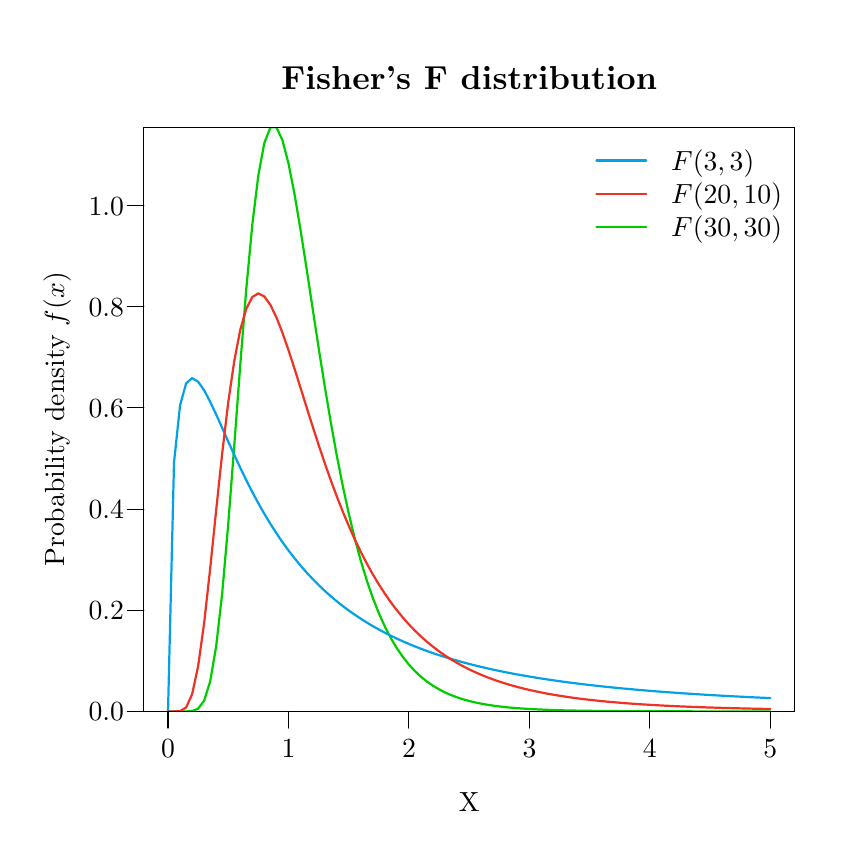
\begin{tikzpicture}[x=1pt,y=1pt]
\definecolor{fillColor}{RGB}{255,255,255}
\path[use as bounding box,fill=fillColor,fill opacity=0.00] (0,0) rectangle (289.08,289.08);
\begin{scope}
\path[clip] ( 42.00, 42.00) rectangle (277.08,253.08);
\definecolor{drawColor}{RGB}{0,205,0}

\path[draw=drawColor,line width= 0.8pt,line join=round,line cap=round] ( 50.71, 42.00) --
	( 52.88, 42.00) --
	( 55.06, 42.00) --
	( 57.24, 42.01) --
	( 59.41, 42.15) --
	( 61.59, 42.98) --
	( 63.77, 45.88) --
	( 65.94, 52.83) --
	( 68.12, 65.59) --
	( 70.30, 84.81) --
	( 72.47,109.69) --
	( 74.65,138.11) --
	( 76.83,167.37) --
	( 79.00,194.73) --
	( 81.18,218.02) --
	( 83.36,235.81) --
	( 85.53,247.47) --
	( 87.71,253.04) --
	( 89.89,253.08) --
	( 92.06,248.42) --
	( 94.24,240.04) --
	( 96.42,228.94) --
	( 98.59,216.01) --
	(100.77,202.06) --
	(102.95,187.72) --
	(105.12,173.50) --
	(107.30,159.77) --
	(109.48,146.78) --
	(111.65,134.71) --
	(113.83,123.63) --
	(116.01,113.57) --
	(118.18,104.53) --
	(120.36, 96.47) --
	(122.54, 89.32) --
	(124.71, 83.02) --
	(126.89, 77.50) --
	(129.07, 72.67) --
	(131.24, 68.47) --
	(133.42, 64.82) --
	(135.60, 61.66) --
	(137.77, 58.92) --
	(139.95, 56.56) --
	(142.13, 54.53) --
	(144.30, 52.78) --
	(146.48, 51.27) --
	(148.66, 49.97) --
	(150.83, 48.86) --
	(153.01, 47.91) --
	(155.19, 47.08) --
	(157.36, 46.38) --
	(159.54, 45.77) --
	(161.72, 45.25) --
	(163.89, 44.81) --
	(166.07, 44.42) --
	(168.25, 44.09) --
	(170.42, 43.81) --
	(172.60, 43.56) --
	(174.78, 43.35) --
	(176.95, 43.17) --
	(179.13, 43.02) --
	(181.31, 42.88) --
	(183.48, 42.77) --
	(185.66, 42.67) --
	(187.84, 42.58) --
	(190.01, 42.50) --
	(192.19, 42.44) --
	(194.37, 42.38) --
	(196.54, 42.33) --
	(198.72, 42.29) --
	(200.90, 42.25) --
	(203.07, 42.22) --
	(205.25, 42.20) --
	(207.43, 42.17) --
	(209.60, 42.15) --
	(211.78, 42.13) --
	(213.96, 42.12) --
	(216.13, 42.10) --
	(218.31, 42.09) --
	(220.49, 42.08) --
	(222.66, 42.07) --
	(224.84, 42.06) --
	(227.02, 42.05) --
	(229.19, 42.05) --
	(231.37, 42.04) --
	(233.55, 42.04) --
	(235.72, 42.03) --
	(237.90, 42.03) --
	(240.08, 42.03) --
	(242.25, 42.02) --
	(244.43, 42.02) --
	(246.61, 42.02) --
	(248.78, 42.02) --
	(250.96, 42.01) --
	(253.14, 42.01) --
	(255.31, 42.01) --
	(257.49, 42.01) --
	(259.67, 42.01) --
	(261.84, 42.01) --
	(264.02, 42.01) --
	(266.20, 42.01) --
	(268.37, 42.01);
\end{scope}
\begin{scope}
\path[clip] (  0.00,  0.00) rectangle (289.08,289.08);
\definecolor{drawColor}{RGB}{0,0,0}

\path[draw=drawColor,line width= 0.4pt,line join=round,line cap=round] ( 50.71, 42.00) -- (268.37, 42.00);

\path[draw=drawColor,line width= 0.4pt,line join=round,line cap=round] ( 50.71, 42.00) -- ( 50.71, 36.00);

\path[draw=drawColor,line width= 0.4pt,line join=round,line cap=round] ( 94.24, 42.00) -- ( 94.24, 36.00);

\path[draw=drawColor,line width= 0.4pt,line join=round,line cap=round] (137.77, 42.00) -- (137.77, 36.00);

\path[draw=drawColor,line width= 0.4pt,line join=round,line cap=round] (181.31, 42.00) -- (181.31, 36.00);

\path[draw=drawColor,line width= 0.4pt,line join=round,line cap=round] (224.84, 42.00) -- (224.84, 36.00);

\path[draw=drawColor,line width= 0.4pt,line join=round,line cap=round] (268.37, 42.00) -- (268.37, 36.00);

\node[text=drawColor,anchor=base,inner sep=0pt, outer sep=0pt, scale=  1.00] at ( 50.71, 25.20) {0};

\node[text=drawColor,anchor=base,inner sep=0pt, outer sep=0pt, scale=  1.00] at ( 94.24, 25.20) {1};

\node[text=drawColor,anchor=base,inner sep=0pt, outer sep=0pt, scale=  1.00] at (137.77, 25.20) {2};

\node[text=drawColor,anchor=base,inner sep=0pt, outer sep=0pt, scale=  1.00] at (181.31, 25.20) {3};

\node[text=drawColor,anchor=base,inner sep=0pt, outer sep=0pt, scale=  1.00] at (224.84, 25.20) {4};

\node[text=drawColor,anchor=base,inner sep=0pt, outer sep=0pt, scale=  1.00] at (268.37, 25.20) {5};

\path[draw=drawColor,line width= 0.4pt,line join=round,line cap=round] ( 42.00, 42.00) -- ( 42.00,224.78);

\path[draw=drawColor,line width= 0.4pt,line join=round,line cap=round] ( 42.00, 42.00) -- ( 36.00, 42.00);

\path[draw=drawColor,line width= 0.4pt,line join=round,line cap=round] ( 42.00, 78.56) -- ( 36.00, 78.56);

\path[draw=drawColor,line width= 0.4pt,line join=round,line cap=round] ( 42.00,115.11) -- ( 36.00,115.11);

\path[draw=drawColor,line width= 0.4pt,line join=round,line cap=round] ( 42.00,151.67) -- ( 36.00,151.67);

\path[draw=drawColor,line width= 0.4pt,line join=round,line cap=round] ( 42.00,188.23) -- ( 36.00,188.23);

\path[draw=drawColor,line width= 0.4pt,line join=round,line cap=round] ( 42.00,224.78) -- ( 36.00,224.78);

\node[text=drawColor,anchor=base east,inner sep=0pt, outer sep=0pt, scale=  1.00] at ( 34.80, 38.56) {0.0};

\node[text=drawColor,anchor=base east,inner sep=0pt, outer sep=0pt, scale=  1.00] at ( 34.80, 75.11) {0.2};

\node[text=drawColor,anchor=base east,inner sep=0pt, outer sep=0pt, scale=  1.00] at ( 34.80,111.67) {0.4};

\node[text=drawColor,anchor=base east,inner sep=0pt, outer sep=0pt, scale=  1.00] at ( 34.80,148.23) {0.6};

\node[text=drawColor,anchor=base east,inner sep=0pt, outer sep=0pt, scale=  1.00] at ( 34.80,184.78) {0.8};

\node[text=drawColor,anchor=base east,inner sep=0pt, outer sep=0pt, scale=  1.00] at ( 34.80,221.34) {1.0};

\path[draw=drawColor,line width= 0.4pt,line join=round,line cap=round] ( 42.00, 42.00) --
	(277.08, 42.00) --
	(277.08,253.08) --
	( 42.00,253.08) --
	( 42.00, 42.00);
\end{scope}
\begin{scope}
\path[clip] (  0.00,  0.00) rectangle (289.08,289.08);
\definecolor{drawColor}{RGB}{0,0,0}

\node[text=drawColor,anchor=base,inner sep=0pt, outer sep=0pt, scale=  1.20] at (159.54,266.89) {\bfseries Fisher's F distribution};

\node[text=drawColor,anchor=base,inner sep=0pt, outer sep=0pt, scale=  1.00] at (159.54,  6.00) {X};

\node[text=drawColor,rotate= 90.00,anchor=base,inner sep=0pt, outer sep=0pt, scale=  1.00] at ( 13.20,147.54) {Probability density $f(x)$};
\end{scope}
\begin{scope}
\path[clip] ( 42.00, 42.00) rectangle (277.08,253.08);
\definecolor{drawColor}{RGB}{5,161,230}

\path[draw=drawColor,line width= 0.8pt,line join=round,line cap=round] ( 50.71, 42.00) --
	( 52.88,131.91) --
	( 55.06,152.59) --
	( 57.24,160.53) --
	( 59.41,162.46) --
	( 61.59,161.16) --
	( 63.77,158.04) --
	( 65.94,153.92) --
	( 68.12,149.28) --
	( 70.30,144.42) --
	( 72.47,139.52) --
	( 74.65,134.70) --
	( 76.83,130.02) --
	( 79.00,125.54) --
	( 81.18,121.26) --
	( 83.36,117.21) --
	( 85.53,113.38) --
	( 87.71,109.78) --
	( 89.89,106.38) --
	( 92.06,103.18) --
	( 94.24,100.18) --
	( 96.42, 97.36) --
	( 98.59, 94.71) --
	(100.77, 92.22) --
	(102.95, 89.89) --
	(105.12, 87.69) --
	(107.30, 85.62) --
	(109.48, 83.67) --
	(111.65, 81.84) --
	(113.83, 80.11) --
	(116.01, 78.48) --
	(118.18, 76.95) --
	(120.36, 75.50) --
	(122.54, 74.13) --
	(124.71, 72.83) --
	(126.89, 71.61) --
	(129.07, 70.45) --
	(131.24, 69.35) --
	(133.42, 68.31) --
	(135.60, 67.32) --
	(137.77, 66.38) --
	(139.95, 65.49) --
	(142.13, 64.64) --
	(144.30, 63.84) --
	(146.48, 63.07) --
	(148.66, 62.34) --
	(150.83, 61.64) --
	(153.01, 60.98) --
	(155.19, 60.35) --
	(157.36, 59.74) --
	(159.54, 59.17) --
	(161.72, 58.61) --
	(163.89, 58.09) --
	(166.07, 57.58) --
	(168.25, 57.10) --
	(170.42, 56.64) --
	(172.60, 56.19) --
	(174.78, 55.77) --
	(176.95, 55.36) --
	(179.13, 54.97) --
	(181.31, 54.60) --
	(183.48, 54.24) --
	(185.66, 53.89) --
	(187.84, 53.56) --
	(190.01, 53.24) --
	(192.19, 52.93) --
	(194.37, 52.63) --
	(196.54, 52.35) --
	(198.72, 52.08) --
	(200.90, 51.81) --
	(203.07, 51.56) --
	(205.25, 51.31) --
	(207.43, 51.07) --
	(209.60, 50.84) --
	(211.78, 50.62) --
	(213.96, 50.41) --
	(216.13, 50.20) --
	(218.31, 50.01) --
	(220.49, 49.81) --
	(222.66, 49.63) --
	(224.84, 49.45) --
	(227.02, 49.27) --
	(229.19, 49.10) --
	(231.37, 48.94) --
	(233.55, 48.78) --
	(235.72, 48.63) --
	(237.90, 48.48) --
	(240.08, 48.34) --
	(242.25, 48.20) --
	(244.43, 48.07) --
	(246.61, 47.93) --
	(248.78, 47.81) --
	(250.96, 47.68) --
	(253.14, 47.56) --
	(255.31, 47.45) --
	(257.49, 47.34) --
	(259.67, 47.23) --
	(261.84, 47.12) --
	(264.02, 47.02) --
	(266.20, 46.92) --
	(268.37, 46.82);
\definecolor{drawColor}{RGB}{238,50,36}

\path[draw=drawColor,line width= 0.8pt,line join=round,line cap=round] ( 50.71, 42.00) --
	( 52.88, 42.00) --
	( 55.06, 42.12) --
	( 57.24, 43.41) --
	( 59.41, 48.17) --
	( 61.59, 58.32) --
	( 63.77, 73.99) --
	( 65.94, 93.59) --
	( 68.12,114.80) --
	( 70.30,135.39) --
	( 72.47,153.67) --
	( 74.65,168.66) --
	( 76.83,179.94) --
	( 79.00,187.54) --
	( 81.18,191.76) --
	( 83.36,193.05) --
	( 85.53,191.93) --
	( 87.71,188.89) --
	( 89.89,184.39) --
	( 92.06,178.84) --
	( 94.24,172.57) --
	( 96.42,165.87) --
	( 98.59,158.94) --
	(100.77,151.96) --
	(102.95,145.07) --
	(105.12,138.35) --
	(107.30,131.87) --
	(109.48,125.69) --
	(111.65,119.82) --
	(113.83,114.28) --
	(116.01,109.08) --
	(118.18,104.22) --
	(120.36, 99.68) --
	(122.54, 95.46) --
	(124.71, 91.54) --
	(126.89, 87.90) --
	(129.07, 84.54) --
	(131.24, 81.42) --
	(133.42, 78.55) --
	(135.60, 75.89) --
	(137.77, 73.43) --
	(139.95, 71.17) --
	(142.13, 69.08) --
	(144.30, 67.15) --
	(146.48, 65.37) --
	(148.66, 63.72) --
	(150.83, 62.20) --
	(153.01, 60.80) --
	(155.19, 59.50) --
	(157.36, 58.31) --
	(159.54, 57.20) --
	(161.72, 56.18) --
	(163.89, 55.23) --
	(166.07, 54.35) --
	(168.25, 53.54) --
	(170.42, 52.79) --
	(172.60, 52.09) --
	(174.78, 51.44) --
	(176.95, 50.84) --
	(179.13, 50.29) --
	(181.31, 49.77) --
	(183.48, 49.29) --
	(185.66, 48.84) --
	(187.84, 48.42) --
	(190.01, 48.03) --
	(192.19, 47.67) --
	(194.37, 47.33) --
	(196.54, 47.02) --
	(198.72, 46.73) --
	(200.90, 46.45) --
	(203.07, 46.20) --
	(205.25, 45.96) --
	(207.43, 45.73) --
	(209.60, 45.52) --
	(211.78, 45.33) --
	(213.96, 45.15) --
	(216.13, 44.97) --
	(218.31, 44.81) --
	(220.49, 44.66) --
	(222.66, 44.52) --
	(224.84, 44.39) --
	(227.02, 44.26) --
	(229.19, 44.14) --
	(231.37, 44.03) --
	(233.55, 43.93) --
	(235.72, 43.83) --
	(237.90, 43.74) --
	(240.08, 43.65) --
	(242.25, 43.57) --
	(244.43, 43.49) --
	(246.61, 43.42) --
	(248.78, 43.35) --
	(250.96, 43.28) --
	(253.14, 43.22) --
	(255.31, 43.16) --
	(257.49, 43.11) --
	(259.67, 43.06) --
	(261.84, 43.01) --
	(264.02, 42.96) --
	(266.20, 42.92) --
	(268.37, 42.88);
\definecolor{drawColor}{RGB}{5,161,230}

\path[draw=drawColor,line width= 0.8pt,line join=round,line cap=round] (205.54,241.08) -- (223.54,241.08);
\definecolor{drawColor}{RGB}{238,50,36}

\path[draw=drawColor,line width= 0.8pt,line join=round,line cap=round] (205.54,229.08) -- (223.54,229.08);
\definecolor{drawColor}{RGB}{0,205,0}

\path[draw=drawColor,line width= 0.8pt,line join=round,line cap=round] (205.54,217.08) -- (223.54,217.08);
\definecolor{drawColor}{RGB}{0,0,0}

\node[text=drawColor,anchor=base west,inner sep=0pt, outer sep=0pt, scale=  1.00] at (232.54,237.64) {$F(3,3)$};

\node[text=drawColor,anchor=base west,inner sep=0pt, outer sep=0pt, scale=  1.00] at (232.54,225.64) {$F(20,10)$};

\node[text=drawColor,anchor=base west,inner sep=0pt, outer sep=0pt, scale=  1.00] at (232.54,213.64) {$F(30,30)$};
\end{scope}
\begin{scope}
\path[clip] (  0.00,  0.00) rectangle (289.08,289.08);
\definecolor{drawColor}{RGB}{0,0,0}

\path[draw=drawColor,line width= 0.4pt,line join=round,line cap=round] ( 42.00, 42.00) --
	(277.08, 42.00) --
	(277.08,253.08) --
	( 42.00,253.08) --
	( 42.00, 42.00);
\end{scope}
\end{tikzpicture}
}}
\mode<presentation>{\resizebox{0.6\textwidth}{!}{% Created by tikzDevice version 0.10.1 on 2016-05-08 18:26:22
% !TEX encoding = UTF-8 Unicode
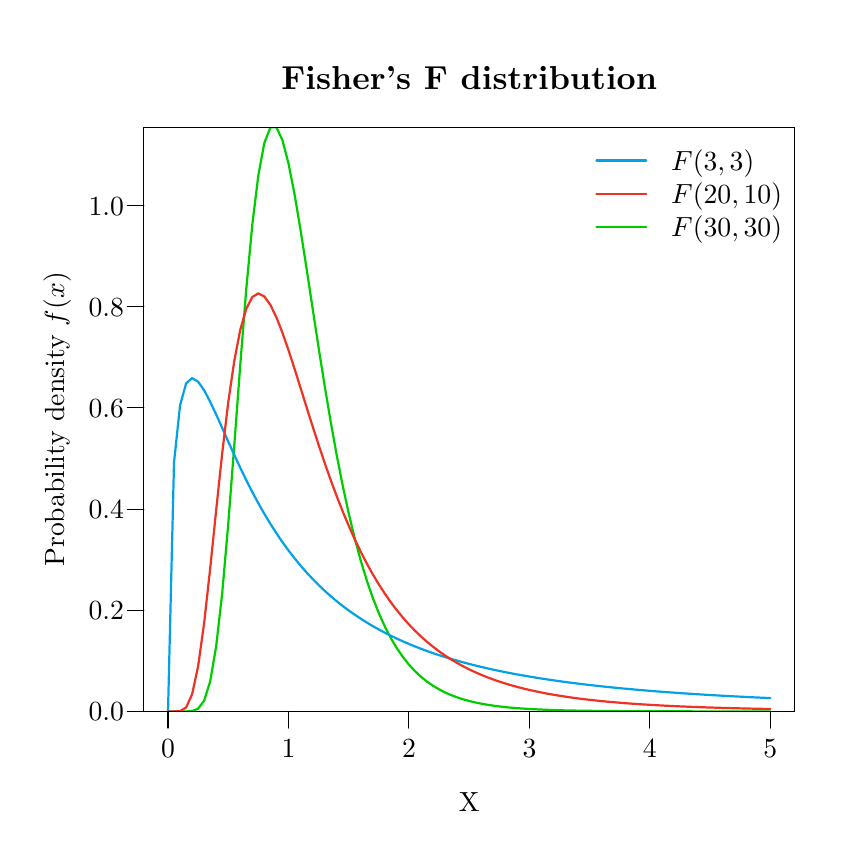
\begin{tikzpicture}[x=1pt,y=1pt]
\definecolor{fillColor}{RGB}{255,255,255}
\path[use as bounding box,fill=fillColor,fill opacity=0.00] (0,0) rectangle (289.08,289.08);
\begin{scope}
\path[clip] ( 42.00, 42.00) rectangle (277.08,253.08);
\definecolor{drawColor}{RGB}{0,205,0}

\path[draw=drawColor,line width= 0.8pt,line join=round,line cap=round] ( 50.71, 42.00) --
	( 52.88, 42.00) --
	( 55.06, 42.00) --
	( 57.24, 42.01) --
	( 59.41, 42.15) --
	( 61.59, 42.98) --
	( 63.77, 45.88) --
	( 65.94, 52.83) --
	( 68.12, 65.59) --
	( 70.30, 84.81) --
	( 72.47,109.69) --
	( 74.65,138.11) --
	( 76.83,167.37) --
	( 79.00,194.73) --
	( 81.18,218.02) --
	( 83.36,235.81) --
	( 85.53,247.47) --
	( 87.71,253.04) --
	( 89.89,253.08) --
	( 92.06,248.42) --
	( 94.24,240.04) --
	( 96.42,228.94) --
	( 98.59,216.01) --
	(100.77,202.06) --
	(102.95,187.72) --
	(105.12,173.50) --
	(107.30,159.77) --
	(109.48,146.78) --
	(111.65,134.71) --
	(113.83,123.63) --
	(116.01,113.57) --
	(118.18,104.53) --
	(120.36, 96.47) --
	(122.54, 89.32) --
	(124.71, 83.02) --
	(126.89, 77.50) --
	(129.07, 72.67) --
	(131.24, 68.47) --
	(133.42, 64.82) --
	(135.60, 61.66) --
	(137.77, 58.92) --
	(139.95, 56.56) --
	(142.13, 54.53) --
	(144.30, 52.78) --
	(146.48, 51.27) --
	(148.66, 49.97) --
	(150.83, 48.86) --
	(153.01, 47.91) --
	(155.19, 47.08) --
	(157.36, 46.38) --
	(159.54, 45.77) --
	(161.72, 45.25) --
	(163.89, 44.81) --
	(166.07, 44.42) --
	(168.25, 44.09) --
	(170.42, 43.81) --
	(172.60, 43.56) --
	(174.78, 43.35) --
	(176.95, 43.17) --
	(179.13, 43.02) --
	(181.31, 42.88) --
	(183.48, 42.77) --
	(185.66, 42.67) --
	(187.84, 42.58) --
	(190.01, 42.50) --
	(192.19, 42.44) --
	(194.37, 42.38) --
	(196.54, 42.33) --
	(198.72, 42.29) --
	(200.90, 42.25) --
	(203.07, 42.22) --
	(205.25, 42.20) --
	(207.43, 42.17) --
	(209.60, 42.15) --
	(211.78, 42.13) --
	(213.96, 42.12) --
	(216.13, 42.10) --
	(218.31, 42.09) --
	(220.49, 42.08) --
	(222.66, 42.07) --
	(224.84, 42.06) --
	(227.02, 42.05) --
	(229.19, 42.05) --
	(231.37, 42.04) --
	(233.55, 42.04) --
	(235.72, 42.03) --
	(237.90, 42.03) --
	(240.08, 42.03) --
	(242.25, 42.02) --
	(244.43, 42.02) --
	(246.61, 42.02) --
	(248.78, 42.02) --
	(250.96, 42.01) --
	(253.14, 42.01) --
	(255.31, 42.01) --
	(257.49, 42.01) --
	(259.67, 42.01) --
	(261.84, 42.01) --
	(264.02, 42.01) --
	(266.20, 42.01) --
	(268.37, 42.01);
\end{scope}
\begin{scope}
\path[clip] (  0.00,  0.00) rectangle (289.08,289.08);
\definecolor{drawColor}{RGB}{0,0,0}

\path[draw=drawColor,line width= 0.4pt,line join=round,line cap=round] ( 50.71, 42.00) -- (268.37, 42.00);

\path[draw=drawColor,line width= 0.4pt,line join=round,line cap=round] ( 50.71, 42.00) -- ( 50.71, 36.00);

\path[draw=drawColor,line width= 0.4pt,line join=round,line cap=round] ( 94.24, 42.00) -- ( 94.24, 36.00);

\path[draw=drawColor,line width= 0.4pt,line join=round,line cap=round] (137.77, 42.00) -- (137.77, 36.00);

\path[draw=drawColor,line width= 0.4pt,line join=round,line cap=round] (181.31, 42.00) -- (181.31, 36.00);

\path[draw=drawColor,line width= 0.4pt,line join=round,line cap=round] (224.84, 42.00) -- (224.84, 36.00);

\path[draw=drawColor,line width= 0.4pt,line join=round,line cap=round] (268.37, 42.00) -- (268.37, 36.00);

\node[text=drawColor,anchor=base,inner sep=0pt, outer sep=0pt, scale=  1.00] at ( 50.71, 25.20) {0};

\node[text=drawColor,anchor=base,inner sep=0pt, outer sep=0pt, scale=  1.00] at ( 94.24, 25.20) {1};

\node[text=drawColor,anchor=base,inner sep=0pt, outer sep=0pt, scale=  1.00] at (137.77, 25.20) {2};

\node[text=drawColor,anchor=base,inner sep=0pt, outer sep=0pt, scale=  1.00] at (181.31, 25.20) {3};

\node[text=drawColor,anchor=base,inner sep=0pt, outer sep=0pt, scale=  1.00] at (224.84, 25.20) {4};

\node[text=drawColor,anchor=base,inner sep=0pt, outer sep=0pt, scale=  1.00] at (268.37, 25.20) {5};

\path[draw=drawColor,line width= 0.4pt,line join=round,line cap=round] ( 42.00, 42.00) -- ( 42.00,224.78);

\path[draw=drawColor,line width= 0.4pt,line join=round,line cap=round] ( 42.00, 42.00) -- ( 36.00, 42.00);

\path[draw=drawColor,line width= 0.4pt,line join=round,line cap=round] ( 42.00, 78.56) -- ( 36.00, 78.56);

\path[draw=drawColor,line width= 0.4pt,line join=round,line cap=round] ( 42.00,115.11) -- ( 36.00,115.11);

\path[draw=drawColor,line width= 0.4pt,line join=round,line cap=round] ( 42.00,151.67) -- ( 36.00,151.67);

\path[draw=drawColor,line width= 0.4pt,line join=round,line cap=round] ( 42.00,188.23) -- ( 36.00,188.23);

\path[draw=drawColor,line width= 0.4pt,line join=round,line cap=round] ( 42.00,224.78) -- ( 36.00,224.78);

\node[text=drawColor,anchor=base east,inner sep=0pt, outer sep=0pt, scale=  1.00] at ( 34.80, 38.56) {0.0};

\node[text=drawColor,anchor=base east,inner sep=0pt, outer sep=0pt, scale=  1.00] at ( 34.80, 75.11) {0.2};

\node[text=drawColor,anchor=base east,inner sep=0pt, outer sep=0pt, scale=  1.00] at ( 34.80,111.67) {0.4};

\node[text=drawColor,anchor=base east,inner sep=0pt, outer sep=0pt, scale=  1.00] at ( 34.80,148.23) {0.6};

\node[text=drawColor,anchor=base east,inner sep=0pt, outer sep=0pt, scale=  1.00] at ( 34.80,184.78) {0.8};

\node[text=drawColor,anchor=base east,inner sep=0pt, outer sep=0pt, scale=  1.00] at ( 34.80,221.34) {1.0};

\path[draw=drawColor,line width= 0.4pt,line join=round,line cap=round] ( 42.00, 42.00) --
	(277.08, 42.00) --
	(277.08,253.08) --
	( 42.00,253.08) --
	( 42.00, 42.00);
\end{scope}
\begin{scope}
\path[clip] (  0.00,  0.00) rectangle (289.08,289.08);
\definecolor{drawColor}{RGB}{0,0,0}

\node[text=drawColor,anchor=base,inner sep=0pt, outer sep=0pt, scale=  1.20] at (159.54,266.89) {\bfseries Fisher's F distribution};

\node[text=drawColor,anchor=base,inner sep=0pt, outer sep=0pt, scale=  1.00] at (159.54,  6.00) {X};

\node[text=drawColor,rotate= 90.00,anchor=base,inner sep=0pt, outer sep=0pt, scale=  1.00] at ( 13.20,147.54) {Probability density $f(x)$};
\end{scope}
\begin{scope}
\path[clip] ( 42.00, 42.00) rectangle (277.08,253.08);
\definecolor{drawColor}{RGB}{5,161,230}

\path[draw=drawColor,line width= 0.8pt,line join=round,line cap=round] ( 50.71, 42.00) --
	( 52.88,131.91) --
	( 55.06,152.59) --
	( 57.24,160.53) --
	( 59.41,162.46) --
	( 61.59,161.16) --
	( 63.77,158.04) --
	( 65.94,153.92) --
	( 68.12,149.28) --
	( 70.30,144.42) --
	( 72.47,139.52) --
	( 74.65,134.70) --
	( 76.83,130.02) --
	( 79.00,125.54) --
	( 81.18,121.26) --
	( 83.36,117.21) --
	( 85.53,113.38) --
	( 87.71,109.78) --
	( 89.89,106.38) --
	( 92.06,103.18) --
	( 94.24,100.18) --
	( 96.42, 97.36) --
	( 98.59, 94.71) --
	(100.77, 92.22) --
	(102.95, 89.89) --
	(105.12, 87.69) --
	(107.30, 85.62) --
	(109.48, 83.67) --
	(111.65, 81.84) --
	(113.83, 80.11) --
	(116.01, 78.48) --
	(118.18, 76.95) --
	(120.36, 75.50) --
	(122.54, 74.13) --
	(124.71, 72.83) --
	(126.89, 71.61) --
	(129.07, 70.45) --
	(131.24, 69.35) --
	(133.42, 68.31) --
	(135.60, 67.32) --
	(137.77, 66.38) --
	(139.95, 65.49) --
	(142.13, 64.64) --
	(144.30, 63.84) --
	(146.48, 63.07) --
	(148.66, 62.34) --
	(150.83, 61.64) --
	(153.01, 60.98) --
	(155.19, 60.35) --
	(157.36, 59.74) --
	(159.54, 59.17) --
	(161.72, 58.61) --
	(163.89, 58.09) --
	(166.07, 57.58) --
	(168.25, 57.10) --
	(170.42, 56.64) --
	(172.60, 56.19) --
	(174.78, 55.77) --
	(176.95, 55.36) --
	(179.13, 54.97) --
	(181.31, 54.60) --
	(183.48, 54.24) --
	(185.66, 53.89) --
	(187.84, 53.56) --
	(190.01, 53.24) --
	(192.19, 52.93) --
	(194.37, 52.63) --
	(196.54, 52.35) --
	(198.72, 52.08) --
	(200.90, 51.81) --
	(203.07, 51.56) --
	(205.25, 51.31) --
	(207.43, 51.07) --
	(209.60, 50.84) --
	(211.78, 50.62) --
	(213.96, 50.41) --
	(216.13, 50.20) --
	(218.31, 50.01) --
	(220.49, 49.81) --
	(222.66, 49.63) --
	(224.84, 49.45) --
	(227.02, 49.27) --
	(229.19, 49.10) --
	(231.37, 48.94) --
	(233.55, 48.78) --
	(235.72, 48.63) --
	(237.90, 48.48) --
	(240.08, 48.34) --
	(242.25, 48.20) --
	(244.43, 48.07) --
	(246.61, 47.93) --
	(248.78, 47.81) --
	(250.96, 47.68) --
	(253.14, 47.56) --
	(255.31, 47.45) --
	(257.49, 47.34) --
	(259.67, 47.23) --
	(261.84, 47.12) --
	(264.02, 47.02) --
	(266.20, 46.92) --
	(268.37, 46.82);
\definecolor{drawColor}{RGB}{238,50,36}

\path[draw=drawColor,line width= 0.8pt,line join=round,line cap=round] ( 50.71, 42.00) --
	( 52.88, 42.00) --
	( 55.06, 42.12) --
	( 57.24, 43.41) --
	( 59.41, 48.17) --
	( 61.59, 58.32) --
	( 63.77, 73.99) --
	( 65.94, 93.59) --
	( 68.12,114.80) --
	( 70.30,135.39) --
	( 72.47,153.67) --
	( 74.65,168.66) --
	( 76.83,179.94) --
	( 79.00,187.54) --
	( 81.18,191.76) --
	( 83.36,193.05) --
	( 85.53,191.93) --
	( 87.71,188.89) --
	( 89.89,184.39) --
	( 92.06,178.84) --
	( 94.24,172.57) --
	( 96.42,165.87) --
	( 98.59,158.94) --
	(100.77,151.96) --
	(102.95,145.07) --
	(105.12,138.35) --
	(107.30,131.87) --
	(109.48,125.69) --
	(111.65,119.82) --
	(113.83,114.28) --
	(116.01,109.08) --
	(118.18,104.22) --
	(120.36, 99.68) --
	(122.54, 95.46) --
	(124.71, 91.54) --
	(126.89, 87.90) --
	(129.07, 84.54) --
	(131.24, 81.42) --
	(133.42, 78.55) --
	(135.60, 75.89) --
	(137.77, 73.43) --
	(139.95, 71.17) --
	(142.13, 69.08) --
	(144.30, 67.15) --
	(146.48, 65.37) --
	(148.66, 63.72) --
	(150.83, 62.20) --
	(153.01, 60.80) --
	(155.19, 59.50) --
	(157.36, 58.31) --
	(159.54, 57.20) --
	(161.72, 56.18) --
	(163.89, 55.23) --
	(166.07, 54.35) --
	(168.25, 53.54) --
	(170.42, 52.79) --
	(172.60, 52.09) --
	(174.78, 51.44) --
	(176.95, 50.84) --
	(179.13, 50.29) --
	(181.31, 49.77) --
	(183.48, 49.29) --
	(185.66, 48.84) --
	(187.84, 48.42) --
	(190.01, 48.03) --
	(192.19, 47.67) --
	(194.37, 47.33) --
	(196.54, 47.02) --
	(198.72, 46.73) --
	(200.90, 46.45) --
	(203.07, 46.20) --
	(205.25, 45.96) --
	(207.43, 45.73) --
	(209.60, 45.52) --
	(211.78, 45.33) --
	(213.96, 45.15) --
	(216.13, 44.97) --
	(218.31, 44.81) --
	(220.49, 44.66) --
	(222.66, 44.52) --
	(224.84, 44.39) --
	(227.02, 44.26) --
	(229.19, 44.14) --
	(231.37, 44.03) --
	(233.55, 43.93) --
	(235.72, 43.83) --
	(237.90, 43.74) --
	(240.08, 43.65) --
	(242.25, 43.57) --
	(244.43, 43.49) --
	(246.61, 43.42) --
	(248.78, 43.35) --
	(250.96, 43.28) --
	(253.14, 43.22) --
	(255.31, 43.16) --
	(257.49, 43.11) --
	(259.67, 43.06) --
	(261.84, 43.01) --
	(264.02, 42.96) --
	(266.20, 42.92) --
	(268.37, 42.88);
\definecolor{drawColor}{RGB}{5,161,230}

\path[draw=drawColor,line width= 0.8pt,line join=round,line cap=round] (205.54,241.08) -- (223.54,241.08);
\definecolor{drawColor}{RGB}{238,50,36}

\path[draw=drawColor,line width= 0.8pt,line join=round,line cap=round] (205.54,229.08) -- (223.54,229.08);
\definecolor{drawColor}{RGB}{0,205,0}

\path[draw=drawColor,line width= 0.8pt,line join=round,line cap=round] (205.54,217.08) -- (223.54,217.08);
\definecolor{drawColor}{RGB}{0,0,0}

\node[text=drawColor,anchor=base west,inner sep=0pt, outer sep=0pt, scale=  1.00] at (232.54,237.64) {$F(3,3)$};

\node[text=drawColor,anchor=base west,inner sep=0pt, outer sep=0pt, scale=  1.00] at (232.54,225.64) {$F(20,10)$};

\node[text=drawColor,anchor=base west,inner sep=0pt, outer sep=0pt, scale=  1.00] at (232.54,213.64) {$F(30,30)$};
\end{scope}
\begin{scope}
\path[clip] (  0.00,  0.00) rectangle (289.08,289.08);
\definecolor{drawColor}{RGB}{0,0,0}

\path[draw=drawColor,line width= 0.4pt,line join=round,line cap=round] ( 42.00, 42.00) --
	(277.08, 42.00) --
	(277.08,253.08) --
	( 42.00,253.08) --
	( 42.00, 42.00);
\end{scope}
\end{tikzpicture}
}}
\end{center}
\end{frame}


%---------------------------------------------------------------------slide----
\begin{frame}
\frametitle{Fisher-Snedecor's F distribution properties}
\begin{itemize}
\item The range is non-negative.
\item It satisfies
\[
F(m,n) =\frac{1}{F(n,m)}.
\]
Thus, if we name $f(m,n)_p$ the value that satisfies $P(F(m,n)\leq f(m,n)_p)=p$, then
\[
f(m,n)_p =\frac{1}{f(n,m)_{1-p}}
\]
which is helpful in order to compute probabilities from the table of the distribution function.
\end{itemize}

\end{frame}

